\documentclass[]{dukedissertation2023}

%\documentclass[economy,twoside,bind]{dukedissertation}
% Use the second for a single-spaced copy suitable for duplex printing
% and binding.

% Other useful options (there are more options documented in Chapter 2):
%  * draft -- don't actually include images, print a black bar on overful
%             hboxes
%  * MS    -- Format for a Master's Thesis.  No UMI abstract page, some 
%             textual changes to title page.  


% Useful packages for dissertation writing:
\usepackage[T1]{fontenc}
\usepackage{titlesec}
\usepackage{amsmath, amssymb, amsfonts, amsthm, stmaryrd}
\usepackage[scr=rsfs]{mathalpha}
\usepackage{upgreek}
\usepackage{bm}
\usepackage{graphicx}
\usepackage[backend=biber,natbib,style=apa,]{biblatex}
\usepackage[title,titletoc]{appendix}
\usepackage{apptools}
%\usepackage{mathptmx} % Uncomment this to use Times instead of Palatino
\usepackage{color}
% \usepackage{mathabx} %If using Times, comment this out
\usepackage{multirow}
\usepackage{setspace}

% \usepackage{mathpazo} % Comment this out if you want to use Times instead of Pallatino
\usepackage{indentfirst}
\usepackage{enumitem}
% \usepackage{xfrac}
\usepackage{mathtools}
\usepackage{caption}
\usepackage{subcaption}
\usepackage{tabularx}
\usepackage{booktabs}
\usepackage{siunitx}
%\usepackage{lscape}
% Use the pdflscape package if you want the page to rotate
\usepackage{pdflscape}
%\usepackage{longtable}
\usepackage{listings}
\usepackage{xcolor}
\usepackage{pgfplots}\pgfplotsset{compat=1.18}
%\usepackage{acronym}
%\usepackage{showframe}
\usepackage{makecell}
\usepackage[super]{nth}
\usepackage{xr}
\usepackage{algorithm}
\usepackage{algpseudocode}

\setlist[itemize]{noitemsep,nolistsep}
\setlist[enumerate]{noitemsep,nolistsep}
\sisetup{per-mode = symbol}
\sisetup{uncertainty-mode = separate}
\sisetup{
	output-open-uncertainty = [,
	output-close-uncertainty = ],
	uncertainty-separator = \,
}

%\usepackage{cite}  % If you include this, hyperlink cites will
                     % break.  It's nice to use this package if your bibstyle
							% sorts entries by order-of-use, rather than
							% alphabetically (as plain does).
							
%Theorem, Lemma, etc. environments
\newtheorem{theorem}{Theorem}%[section]
\newtheorem{lemma}[theorem]{Lemma}
\newtheorem{proposition}[theorem]{Proposition}
\newtheorem{corollary}[theorem]{Corollary}
\newtheorem{result}[theorem]{Result}

% Personal commands and abbreviations.
%Define and personal commands here

%Graphics Path to find your pictures
\graphicspath{{./Pictures/}{./Chapter1}} %Add multiple paths if there are images in multiple spots



%-----------------------------------------------------------------------------%
% PREAMBLE 
%-----------------------------------------------------------------------------%
\author{Peiyi Chen}
\title{[(Test) Your Title Here Even If It Is Very Very Very Very Very Very Long. Truly It Is A Miraculously Long Title For A Dissertation]}
\supervisor{Johann Guilleminot}
\department{Mechanical Engineering and Materials Science} % Appears as Department of \department
% Declare dissertation subject used on UMI abstract page.  List of
% categories: http://dissertations.umi.com/duke/subject_categories.html
%\subject{[Your Subject Here]}

\date{2023} % Anything but the year is ignored.

% Copyright text.  If undefined, default is 'All rights reserved'
% (Example sets the text to a hyperlinked Creative Commons Licence)
\copyrighttext{All rights reserved except the rights granted by the \href{http://creativecommons.org/licenses/by-nc/3.0/us/}{Creative Commons Attribution-Noncommercial Licence}}

% Committee Members other than supervisor.  No more than five beyond the
% supervisor allowed.Do not include titles (e.g. `Dr.')
\defensedate{Feburary 27, 2024}
\member{John Dolbow}
\member{Wilkins Aquino}
\member{Hossein Salahshoor}
% \member{[Committee Member 4]}
% \member{[Committee Member 5]}
%-----------------------------------------------------------------------------%

%-----------------------------------------------------------------------------%
% HYPERREF: plain black hypertext references for ref's and cite's.
%-----------------------------------------------------------------------------%
\usepackage[pdftex, pdfusetitle, plainpages=false, bookmarks, bookmarksnumbered, colorlinks, linkcolor=black, citecolor=black, filecolor=black, urlcolor=black,linktoc=none]{hyperref}
\usepackage[capitalise]{cleveref}
\creflabelformat{equation}{#2#1#3}
\makeatletter

\newcommand\getfontsizeofheading{The current font size is: \fontname\font \f@size pt}
% print given font size in point and in its "font size" (i.e. larger or smaller)
\newcommand\getfontsizeforfontsizeclass[1]{{\string #1 is printed as #1  \fontname\font \f@size pt\par}}
% print the entire string in the size of the fontsize (i.e. larger or smaller)
\newcommand\printfontsizeforfontsizeclass[1]{{#1 \string #1 is printed in  \fontname\font \f@size pt\par}}
\makeatother

%% macro from Peiyi

\newtheorem*{remark}{Remark}
\newtheorem{prop}{Proposition}

%% MACROS
\newcommand\bfa{\boldsymbol{a}}
\newcommand\bfb{\boldsymbol{b}}
\newcommand\bfc{\boldsymbol{c}}
\newcommand\bfd{\boldsymbol{d}}
\newcommand\bfe{\boldsymbol{e}}
\newcommand\bff{\boldsymbol{f}}
\newcommand\bfg{\boldsymbol{g}}
\newcommand\bfh{\boldsymbol{h}}
\newcommand\bfi{\boldsymbol{i}}
\newcommand\bfj{\boldsymbol{j}}
\newcommand\bfk{\boldsymbol{k}}
\newcommand\bfl{\boldsymbol{l}}
\newcommand\bfm{\boldsymbol{m}}
\newcommand\bfn{\boldsymbol{n}}
\newcommand\bfo{\boldsymbol{o}}
\newcommand\bfp{\boldsymbol{p}}
\newcommand\bfq{\boldsymbol{q}}
\newcommand\bfr{\boldsymbol{r}}
\newcommand\bfs{\boldsymbol{s}}
\newcommand\bft{\boldsymbol{t}}
\newcommand\bfu{\boldsymbol{u}}
\newcommand\bfv{\boldsymbol{v}}
\newcommand\bfw{\boldsymbol{w}}
\newcommand\bfx{\boldsymbol{x}}
\newcommand\bfy{\boldsymbol{y}}
\newcommand\bfz{\boldsymbol{z}}
%
\newcommand\bfA{\boldsymbol{A}}
\newcommand\bfB{\boldsymbol{B}}
\newcommand\bfC{\boldsymbol{C}}
\newcommand\bfD{\boldsymbol{D}}
\newcommand\bfE{\boldsymbol{E}}
\newcommand\bfF{\boldsymbol{F}}
\newcommand\bfG{\boldsymbol{G}}
\newcommand\bfH{\boldsymbol{H}}
\newcommand\bfI{\boldsymbol{I}}
\newcommand\bfJ{\boldsymbol{J}}
\newcommand\bfK{\boldsymbol{K}}
\newcommand\bfL{\boldsymbol{L}}
\newcommand\bfM{\boldsymbol{M}}
\newcommand\bfN{\boldsymbol{N}}
\newcommand\bfO{\boldsymbol{O}}
\newcommand\bfP{\boldsymbol{P}}
\newcommand\bfQ{\boldsymbol{Q}}
\newcommand\bfR{\boldsymbol{R}}
\newcommand\bfS{\boldsymbol{S}}
\newcommand\bfT{\boldsymbol{T}}
\newcommand\bfU{\boldsymbol{U}}
\newcommand\bfV{\boldsymbol{V}}
\newcommand\bfW{\boldsymbol{W}}
\newcommand\bfX{\boldsymbol{X}}
\newcommand\bfY{\boldsymbol{Y}}
\newcommand\bfZ{\boldsymbol{Z}}

\newcommand{\diff}[1]{\text{ d}#1}

\newcommand{\bta}{\textbf{a}}
\newcommand{\btb}{\textbf{b}}
\newcommand{\btc}{\textbf{c}}
\newcommand{\btd}{\textbf{d}}
\newcommand{\bte}{\textbf{e}}
\newcommand{\btf}{\textbf{f}}
\newcommand{\btg}{\textbf{g}}
\newcommand{\bth}{\textbf{h}}
\newcommand{\bti}{\textbf{i}}
\newcommand{\btj}{\textbf{j}}
\newcommand{\btk}{\textbf{k}}
\newcommand{\btl}{\textbf{l}}
\newcommand{\btm}{\textbf{m}}
\newcommand{\btn}{\textbf{n}}
\newcommand{\bto}{\textbf{o}}
\newcommand{\btp}{\textbf{p}}
\newcommand{\btq}{\textbf{q}}
\newcommand{\btr}{\textbf{r}}
\newcommand{\bts}{\textbf{s}}
\newcommand{\btt}{\textbf{t}}
\newcommand{\btu}{\textbf{u}}
\newcommand{\btv}{\textbf{v}}
\newcommand{\btw}{\textbf{w}}
\newcommand{\btx}{\textbf{x}}
\newcommand{\bty}{\textbf{y}}
\newcommand{\btz}{\textbf{z}}

\newcommand{\btA}{\textbf{A}}
\newcommand{\btB}{\textbf{B}}
\newcommand{\btC}{\textbf{C}}
\newcommand{\btD}{\textbf{D}}
\newcommand{\btE}{\textbf{E}}
\newcommand{\btF}{\textbf{F}}
\newcommand{\btG}{\textbf{G}}
\newcommand{\btH}{\textbf{H}}
\newcommand{\btI}{\textbf{I}}
\newcommand{\btJ}{\textbf{J}}
\newcommand{\btK}{\textbf{K}}
\newcommand{\btL}{\textbf{L}}
\newcommand{\btM}{\textbf{M}}
\newcommand{\btN}{\textbf{N}}
\newcommand{\btO}{\textbf{O}}
\newcommand{\btP}{\textbf{P}}
\newcommand{\btQ}{\textbf{Q}}
\newcommand{\btR}{\textbf{R}}
\newcommand{\btS}{\textbf{S}}
\newcommand{\btT}{\textbf{T}}
\newcommand{\btU}{\textbf{U}}
\newcommand{\btV}{\textbf{V}}
\newcommand{\btW}{\textbf{W}}
\newcommand{\btX}{\textbf{X}}
\newcommand{\btY}{\textbf{Y}}
\newcommand{\btZ}{\textbf{Z}}

\newcommand{\rta}{\text{a}}
\newcommand{\rtb}{\text{b}}
\newcommand{\rtc}{\text{c}}
\newcommand{\rtd}{\text{d}}
\newcommand{\rte}{\text{e}}
\newcommand{\rtf}{\text{f}}
\newcommand{\rtg}{\text{g}}
\newcommand{\rth}{\text{h}}
\newcommand{\rti}{\text{i}}
\newcommand{\rtj}{\text{j}}
\newcommand{\rtk}{\text{k}}
\newcommand{\rtl}{\text{l}}
\newcommand{\rtm}{\text{m}}
\newcommand{\rtn}{\text{n}}
\newcommand{\rto}{\text{o}}
\newcommand{\rtp}{\text{p}}
\newcommand{\rtq}{\text{q}}
\newcommand{\rtr}{\text{r}}
\newcommand{\rts}{\text{s}}
\newcommand{\rtt}{\text{t}}
\newcommand{\rtu}{\text{u}}
\newcommand{\rtv}{\text{v}}
\newcommand{\rtw}{\text{w}}
\newcommand{\rtx}{\text{x}}
\newcommand{\rty}{\text{y}}
\newcommand{\rtz}{\text{z}}

\newcommand{\rtA}{\text{A}}
\newcommand{\rtB}{\text{B}}
\newcommand{\rtC}{\text{C}}
\newcommand{\rtD}{\text{D}}
\newcommand{\rtE}{\text{E}}
\newcommand{\rtF}{\text{F}}
\newcommand{\rtG}{\text{G}}
\newcommand{\rtH}{\text{H}}
\newcommand{\rtI}{\text{I}}
\newcommand{\rtJ}{\text{J}}
\newcommand{\rtK}{\text{K}}
\newcommand{\rtL}{\text{L}}
\newcommand{\rtM}{\text{M}}
\newcommand{\rtN}{\text{N}}
\newcommand{\rtO}{\text{O}}
\newcommand{\rtP}{\text{P}}
\newcommand{\rtQ}{\text{Q}}
\newcommand{\rtR}{\text{R}}
\newcommand{\rtS}{\text{S}}
\newcommand{\rtT}{\text{T}}
\newcommand{\rtU}{\text{U}}
\newcommand{\rtV}{\text{V}}
\newcommand{\rtW}{\text{W}}
\newcommand{\rtX}{\text{X}}
\newcommand{\rtY}{\text{Y}}
\newcommand{\rtZ}{\text{Z}}

\DeclareMathOperator*{\argmin}{argmin}

%
\newcommand\bs[1]{\boldsymbol{#1}}

\newcommand{\defgrad}{\bfF}
\newcommand{\rcg}{\bfC}
\newcommand{\grad}{\boldsymbol{\nabla}}
\DeclareMathOperator{\tr}{tr}
\DeclareMathOperator{\cof}{cof}
\newcommand{\divergence}{\grad \cdot}
\newcommand{\mms}{\text{MMS}}
\newcommand{\cov}{\text{Cov}}

\newcommand{\inner}[3]{\langle#2, #3\rangle_{#1}}
\DeclareMathOperator{\heaviside}{heaviside}
\newcommand{\btphi}{\boldsymbol{\upphi}}
\newcommand{\btPhi}{\boldsymbol{\Upphi}}

\newcommand{\macaulay}[1]{{\left<#1\right>}}
\newcommand{\norm}[1]{{\left\lVert#1\right\rVert}}
% \newcommand\hmmax{0}
% \newcommand\bmmax{0}
%%
%%

%%PLOM
\newcommand{\bfnabla}{{{\boldsymbol{\nabla}}}}
\newcommand{\bfun}{{\boldsymbol{1}}}
\newcommand{\bfzero}{{ \hbox{\bf 0} }}

\newcommand{\bfAlpha}{{\mathbf{\Alpha}}}
\newcommand{\bfBeta}{{\mathbf{\Beta}}}
\newcommand{\bfEpsilon}{{\mathbf{\Epsilon}}}
\newcommand{\bfGamma}{{\mathbf{\Gamma}}}
\newcommand{\bfDelta}{{\mathbf{\Delta}}}
\newcommand{\bfEta}{{\bfH}}
\newcommand{\bfTheta}{{\mathbf{\Theta}}}
\newcommand{\bfLambda}{{\mathbf{\Lambda}}}
\newcommand{\bfMu}{{\mathbf{\Mu}}}
\newcommand{\bfNu}{{\mathbf{\Nu}}}
\newcommand{\bfOmega}{{\mathbf{\Omega}}}
\newcommand{\bfPhi}{{\mathbf{\Phi}}}
\newcommand{\bfPi}{{\mathbf{\Pi}}}
\newcommand{\bfPsi}{{\mathbf{\Psi}}}
\newcommand{\bfXi}{{\mathbf{\Xi}}}
\newcommand{\bfZeta}{{\mathbf{\Zeta}}}
\newcommand{\bfSigma}{{\mathbf{\Sigma}}}
\newcommand{\bfUpsilon}{{\mathbf{\Upsilon}}}

\newcommand{\bfalpha}{{\boldsymbol{\alpha}}}
\newcommand{\bfbeta}{{\boldsymbol{\beta}}}
\newcommand{\bfgamma}{{\boldsymbol{\gamma}}}
\newcommand{\bfdelta}{{\boldsymbol{\delta}}}
\newcommand{\bfeta}{{\boldsymbol{\eta}}}
\newcommand{\bftheta}{{\boldsymbol{\theta}}}
\newcommand{\bflambda}{{\boldsymbol{\lambda}}}
\newcommand{\bfmu}{{\boldsymbol{\mu}}}
\newcommand{\bfnu}{{\boldsymbol{\nu}}}
\newcommand{\bfomega}{{\boldsymbol{\omega}}}
\newcommand{\bfvarphi}{{\boldsymbol{\varphi}}}
\newcommand{\bfpsi}{{\boldsymbol{\psi}}}
\newcommand{\bfxi}{{\boldsymbol{\xi}}}
\newcommand{\bfchi}{{\boldsymbol{\chi}}}
\newcommand{\bfzeta}{{\boldsymbol{\zeta}}}
\newcommand{\bfphi}{{\boldsymbol{\phi}}}
\newcommand{\bfsigma}{{\boldsymbol{\sigma}}}
\newcommand{\bfvarepsilon}{{\boldsymbol{\varepsilon}}}

\newcommand{\Eta}{{\rm H}}

\newcommand{\AAeclair}{{\mathbb{A}}}
\newcommand{\BB}{{\mathbb{B}}}
\newcommand{\CC}{{\mathbb{C}}}
\newcommand{\DD}{{\mathbb{D}}}
\newcommand{\FF}{{\mathbb{F}}}
\newcommand{\GG}{{\mathbb{G}}}
\newcommand{\HH}{{\mathbb{H}}}
\newcommand{\II}{{\mathbb{I}}}
\newcommand{\KK}{{\mathbb{K}}}
\newcommand{\LL}{{\mathbb{L}}}
\newcommand{\MM}{{\mathbb{M}}}
\newcommand{\NN}{{\mathbb{N}}}
\newcommand{\PP}{{\mathbb{P}}}
\newcommand{\QQ}{{\mathbb{Q}}}
\newcommand{\RR}{{\mathbb{R}}}
\newcommand{\SSeclair}{{\mathbb{S}}}
\newcommand{\UU}{{\mathbb{U}}}
\newcommand{\VV}{{\mathbb{V}}}
\newcommand{\WW}{{\mathbb{W}}}
\newcommand{\XX}{{\mathbb{X}}}
\newcommand{\YY}{{\mathbb{Y}}}
\newcommand{\ZZ}{{\mathbb{Z}}}

\newcommand\revised[1]{{\color{blue}{#1}}}
\newcommand\unclear[1]{{\color{red}{#1}}}
\newcommand\comment[1]{{\color{green}{#1}}}

\DeclareMathAlphabet{\mathonebb}{U}{bbold}{m}{n}
\def\11{{\ensuremath{\mathonebb{1}}}}
\def\oo{{\ensuremath{\mathonebb{o}}}}
\def\aa{{\ensuremath{\mathonebb{a}}}}
\def\bb{{\ensuremath{\mathonebb{b}}}}
\def\ee{{\ensuremath{\mathonebb{e}}}}
\def\ff{{\ensuremath{\mathonebb{f}}}}
\def\hh{{\ensuremath{\mathonebb{h}}}}
\def\mm{{\ensuremath{\mathonebb{m}}}}
\def\qq{{\ensuremath{\mathonebb{q}}}}
\def\rr{{\ensuremath{\mathonebb{r}}}}
\def\ss{{\ensuremath{\mathonebb{s}}}}
\def\uu{{\ensuremath{\mathonebb{u}}}}
\def\yy{{\ensuremath{\mathonebb{y}}}}
\def\ww{{\ensuremath{\mathonebb{w}}}}
\def\xx{{\ensuremath{\mathonebb{x}}}}
\def\PhiPhi{{\ensuremath{\mathonebb{\Phi}}}}

\newcommand{\curA}{{\mathcal{A}}}
\newcommand{\curB}{{\mathcal{B}}}
\newcommand{\curC}{{\mathcal{C}}}
\newcommand{\curD}{{\mathcal{D}}}
\newcommand{\curE}{{\mathcal{E}}}
\newcommand{\curG}{{\mathcal{G}}}
\newcommand{\curH}{{\mathcal{H}}}
\newcommand{\curI}{{\mathcal{I}}}
\newcommand{\curJ}{{\mathcal{J}}}
\newcommand{\curK}{{\mathcal{K}}}
\newcommand{\curL}{{\mathcal{L}}}
\newcommand{\curM}{{\mathcal{M}}}
\newcommand{\curN}{{\mathcal{N}}}
\newcommand{\curP}{{\mathcal{P}}}
\newcommand{\curQ}{{\mathcal{Q}}}
\newcommand{\curR}{{\mathcal{R}}}
\newcommand{\curS}{{\mathcal{S}}}
\newcommand{\curT}{{\mathcal{T}}}
\newcommand{\curU}{{\mathcal{U}}}
\newcommand{\curV}{{\mathcal{V}}}
\newcommand{\curW}{{\mathcal{W}}}
\newcommand{\curX}{{\mathcal{X}}}
\newcommand{\curY}{{\mathcal{Y}}}
\newcommand{\curZ}{{\mathcal{Z}}}

%
\newcommand{\bfcurA}{\boldsymbol{\mathcal{A}}}
\newcommand{\bfcurB}{\boldsymbol{\mathcal{B}}}
\newcommand{\bfcurC}{\boldsymbol{\mathcal{C}}}
\newcommand{\bfcurD}{\boldsymbol{\mathcal{D}}}
\newcommand{\bfcurE}{\boldsymbol{\mathcal{E}}}
\newcommand{\bfcurF}{\boldsymbol{\mathcal{F}}}
\newcommand{\bfcurG}{\boldsymbol{\mathcal{G}}}
\newcommand{\bfcurH}{\boldsymbol{\mathcal{H}}}
\newcommand{\bfcurI}{\boldsymbol{\mathcal{I}}}
\newcommand{\bfcurJ}{\boldsymbol{\mathcal{J}}}
\newcommand{\bfcurK}{\boldsymbol{\mathcal{K}}}
\newcommand{\bfcurL}{\boldsymbol{\mathcal{L}}}
\newcommand{\bfcurM}{\boldsymbol{\mathcal{M}}}
\newcommand{\bfcurN}{\boldsymbol{\mathcal{N}}}
\newcommand{\bfcurO}{\boldsymbol{\mathcal{O}}}
\newcommand{\bfcurP}{\boldsymbol{\mathcal{P}}}
\newcommand{\bfcurQ}{\boldsymbol{\mathcal{Q}}}
\newcommand{\bfcurR}{\boldsymbol{\mathcal{R}}}
\newcommand{\bfcurS}{\boldsymbol{\mathcal{S}}}
\newcommand{\bfcurT}{\boldsymbol{\mathcal{T}}}
\newcommand{\bfcurU}{\boldsymbol{\mathcal{U}}}
\newcommand{\bfcurV}{\boldsymbol{\mathcal{V}}}
\newcommand{\bfcurW}{\boldsymbol{\mathcal{W}}}
\newcommand{\bfcurX}{\boldsymbol{\mathcal{X}}}
\newcommand{\bfcurY}{\boldsymbol{\mathcal{Y}}}
\newcommand{\bfcurZ}{\boldsymbol{\mathcal{Z}}}

\AtBeginBibliography{\vspace*{\baselineskip}}
\setlength{\bibitemsep}{\baselineskip}

%\titleformat{\chapter}
%	{\Large\bfseries\usefont{T1}{phv}{b}{n}\fontsize{16pt}{\baselineskip}} %Format
%	{\thechapter.} %Label
%	{\fontdimen2\font\space} %Sep
%	{\normalbaselines} % Before 

%\renewcommand{\thesection}{\arabic{chapter}.\arabic{section}}
%\renewcommand{\thesubsection}{\arabic{chapter}.\arabic{section}.\arabic{subsection}}
%\renewcommand{\thesubsubsection}{\arabic{chapter}.\arabic{section}.\arabic{subsection}.\arabic{subsubsection}}

\titleformat{\section}[block]{\fontencoding{T1}\fontfamily{phv}\fontseries{b}%
  \fontshape{it}\fontsize{14pt}{11}\selectfont}{\thesection}{.2em}{\normalbaselines}
 \titleformat{\subsection}[block]{\fontencoding{T1}\fontfamily{phv}\fontseries{b}%
  \fontshape{n}\fontsize{13pt}{11}\selectfont}{\thesubsection}{.2em}{\normalbaselines}
 \titleformat{\subsubsection}[block]{\fontencoding{T1}\fontfamily{ppl}\fontseries{b}%
  \fontshape{n}\fontsize{11pt}{11}\selectfont}{\thesubsubsection}{.2em}{\normalbaselines}
  
  
\titlespacing\section{0pt}{14pt plus 0pt minus 0pt}{6pt plus 0pt minus 0pt}
\titlespacing\subsection{0pt}{14pt plus 0pt minus 0pt}{6pt plus 0pt minus 0pt}
\titlespacing\subsubsection{0pt}{14pt plus 0pt minus 0pt}{6pt plus 0pt minus 0pt}
\titlespacing\paragraph{0pt}{6pt plus 0pt minus 0pt}{6pt plus 0pt minus 0pt}
\titlespacing\subparagraph{0pt}{6pt plus 0pt minus 0pt}{6pt plus 0pt minus 0pt}

\setcounter{secnumdepth}{4}

\newcolumntype{L}[1]{>{\raggedright\let\newline\\\arraybackslash\hspace{0pt}}b{#1}}
\newcolumntype{C}[1]{>{\centering\let\newline\\\arraybackslash\hspace{0pt}}b{#1}}
\newcolumntype{R}[1]{>{\raggedleft\let\newline\\\arraybackslash\hspace{0pt}}b{#1}}

\usepackage{subfiles}
\addbibresource{./Bibliography/mybib.bib} %your bibliography file - change the path if needed
\begin{document}

%-----------------------------------------------------------------------------%
% TITLE PAGE -- provides UMI abstract title page & copyright if appropriate
%-----------------------------------------------------------------------------%
\maketitle

%-----------------------------------------------------------------------------%
% ABSTRACT -- included file should start with '\abstract'.
%-----------------------------------------------------------------------------%
\abstract
In the abstract, you must (1) present the problem of the thesis/dissertation, (2) discuss the materials and methods used, and (3) state the conclusions reached. Individual chapters should not have abstracts.
 
Note that this will be the first numbered page: it is page \textit{iv}; pages \textit{i}, \textit{ii} and \textit{iii} (copyright, signature page and abstract signature page) were counted but not numbered. If you look ahead, you will see that numbering up to the first page of text is in roman numerals. On the first page of Introduction or Chapter One, begin numbering at Arabic number 1. This numbering (1, 2, 3, 4 \dots) is consecutive through the rest of the document. 

Also note that the page margins are set with a 1.5-inch margin on the left side and a 1-inch margin on the top, right side, and bottom, throughout the entire document.

The page number below should be above the 1-inch margin and centered to the page margins, not the page edges.

%-----------------------------------------------------------------------------%
% DEDICATION -- OPTIONAL.  Put the text inside the braces.
%               (Long 'dedications' probably belong in the acknowledgements)
%-----------------------------------------------------------------------------%
% \dedication{If you want to dedicate your thesis to anyone do so here.}

%-----------------------------------------------------------------------------%
% FRONTMATTER -- ToC is required, LoT and LoF are required if you have any
% tables or figures, respectively. List of Abbreviations and Symbols is 
% optional.
%-----------------------------------------------------------------------------%
\tableofcontents % Automatically generated

\listoftables	% If you have any tables, automatically generated

\listoffigures	% If you have any figures, automatically generated

%\include{./Abbreviations/listofabbr} % List of Abbreviations. Start file with '\abbreviations'

%-----------------------------------------------------------------------------%
% ACKNOWLEDGEMENTS -- included file should start with '\acknowledgements'
%-----------------------------------------------------------------------------%
\acknowledgements

I would like to deeply thank my PhD advisor, Professor Johann Guilleminot, for the wealth of knowledge I have acquired under his guidancethe, and the amazing time that we worked together. He is a wonderful mentor and dedicated coolaborator, and always an inovative researcher. In moments of challenge throughout my doctoral journey, he consistently offers invaluable insights during discussions and provides assistance in resolving issues. His devotion and passion to his research inspired and motivated me to become a committed and serious engineer.

I would like to extend my gratitude to my esteemed collaborator, Professor Christian Soize, whose significant contributions have played a crucial role in bringing this dissertation to completion. I would also like to thank Professor John Dolbow, Professor Wilkins Aquino, Professor Hossein Salahshoor for accepting to evaluate this work.

I acknowledge the financial support of the Graduate School at Duke University. This work was partially funded by the National Science Foundation (NSF) under grants CMMI-1726403, CMMI-1942928, and DGE-2022040.

Last but not least, I thank my fiancé Gary, and my dog Rudy for believing in me and supporting me during all these years.

%==============================================================================
%-----------------------------------------------------------------------------%
%
% MAIN BODY OF PAPER
%
%
%-----------------------------------------------------------------------------%
\chapter{Introduction}
\label{chap:Introduction}

The mathematically-consistent representation and identification of parametric uncertainties is a central task of uncertainty quantification (UQ) in computational mechanics. From a mechanics of materials standpoint \cite{GUILLEMINOT2020385}, such fluctuations can be primarily attributed to subscale variability, which itself---and most often---stems from complex processing conditions for engineered composites (such as fiber-reinforced composites or concrete), or evolution-based optimization in the case of biological tissues. There has been a tremendous amount of works focusing on the integration of such uncertainties in the past three decades. Labeled statistical distributions, such as Gaussian, Gamma, and lognormal distributions, are generally assumed to model homogeneous stochastic inputs. The choice of these distributions is sometimes arbitrarily made or based on data fitting (which may lead to ill-posed forward problems), and can facilitate uncertainty propagation through spectral approaches \cite{Ghanem1991, OLM, Ghanem2017} where quantities of interest are represented by polynomial chaos surrogate models \cite{Wiener,Cameron,Xiu2002,Soize2004}. When an accurate microstructural description is not possible, due to data limitation, prior models can be constructed that capture available physical information, such as anisotropy, as well as mathematical constraints related to well-posedness for the associated forward propagation problem. Information-theoretic contributions proceeding along those lines can be found in \cite{Soize2006,Guilleminot-IJNME-2017,Guilleminot-SIAM-2013,STABER2017399} for the case of tensor-valued coefficients in linear differential operators, to list a few; see also \cite{Grigoriu2016} for yet another type of methodology, as well as \cite{SOIZE2011} for integration within a Bayesian setting.

While traditional approaches have established a solid foundation for uncertainty quantification in computational mechanics, the complex nature of certain materials demands more adaptive and data-driven approaches. Lately, constitutive models based on neural networks (NN) have also received growing attention over the past few years, owing to their ability to represent nonlinear mappings in a high dimensional setting. There is a very substantial amount of papers published on this topic, for a wide variety of material behaviors; see, \textit{e.g.},  \cite{flaschel2021unsupervised,xu2021learning,holzapfel2021predictive,jung2006neural,ghaboussi1998autoprogressive,ghaboussi1998new,hashash2004numerical,furukawa1998implicit,joshi2022bayesian,as2022mechanics,Asad-IJNME,KLEIN2022104703} and the references therein, in a non-exhaustive manner. Beyond classical data science aspects that pertain to architecture design, training and validation strategies, and the analysis of approximation capabilities, a central concern is to make such surrogates amenable to scientific simulations where such models are typically set to parameterize systems of partial differential equations. In this context, the surrogate must satisfy both physical assumptions and mathematical properties (\textit{e.g.}, boundedness or a certain type of convexity) to ensure the existence (and potentially, the uniqueness) of solutions. From the interests of mathematically-consistent representations, where precision and robustness are significant, we know that a high-fidelity simulation, oftentimes in the form of coupled partial differential equations (PDEs), is computationally prohibitive as a feasible forward simulation within the outer loop in many decision-making applications, e.g. inverse problem, optimal control, uncertainty quantification, etc. To avoid evaluating the expensive high-fidelity model in a forward simulation, a reduced order model (ROM) can be trained as its surrogate with reasonable accuracy, hence significantly reducing the computational cost allowing for faster simulations and real-time applications without sacrificing the essence of the underlying mathematical principles. Nonlinear PDEs describe a wide spectrum of engineering problems. High-fidelity numerical solvers based on high-dimensional spatial discretizations are prohibitively expensive in many-query settings. Intrusive and non-intrusive LS-ROMs reduce the dimensionality of the model by projecting the solution of the high-dimensional model onto a linear subspace. Several approaches to defining the approximation subspace have been proposed (see e.g. \cite{benner2015survey} for a review). A common empirical choice is the proper orthogonal decomposition (POD) subspace, which spans the leading principal components of an available set of state data \cite{berkooz1993proper,lumley1967structure,sirovich1987turbulence}. For PDEs with only linear and polynomial terms, the projection-based reduced model admits an efficient low-dimensional numerical representation that can be cheaply evaluated at a cost independent of the dimension of the original model \cite{benner2015two,benner2015survey,cuong2005certified,goyal2016algebraic,hesthaven2016certified}. For PDEs with more general nonlinear terms, an additional level of approximation, e.g., interpolation \cite{astrid2008missing,barrault2004empirical,carlberg2013gnat,chaturantabut2010nonlinear,drmac2016new,grepl2007efficient,nguyen2008best}, is generally needed to achieve computational efficiency. Alternatively, the works in \cite{benner2015two,goyal2016algebraic,kramer2019nonlinear,kramer2019balanced} transform PDEs with general nonlinear terms to representations with only quadratic nonlinearities via the use of structure-exposing lifting transformations, and then project the quadratic operators of the resultant lifted PDE to obtain a reduced model. In recent years, machine learning based approaches to NM-ROMs have received an increasing interest. Some treat the weights and biases of a deep neural network (DNN) as unknowns in the solution process \cite{dissanayake1994neural,lagaris1998artificial,meade1994numerical,van1995neural}, while others incorporate physical laws into DNN-based surrogates whose weights and biases are determined in the training phase \cite{han2018solving,lu2019deeponet,lu2021deepxde,pang2019fpinns,raissi2019physics,lee2020model,lee2019deep}. 

Notet that uncertainties within nonlinear constitutive models can be defined in a multiscale framework where material parameters are made random. Concurrent nonlinear simulations involve the strong coupling between a macroscopic (or structural) formulation and a microscopic description capturing subscale details \cite{ghosh1996two,smit1998prediction,feyel1999multiscale,feyel2000fe2,terada2001class,kouznetsova2002multi,geers2016multiscale,raju2021review}. One popular approach is the so-called FE$^2$ method \cite{feyel1999multiscale,feyel2000fe2}, where information (in the form of a deformation gradient and any adapted stress variable) is transferred back-and-forth between quadrature points at the macroscale and statistical or representative volume elements (depending on whether the separation of scales exists or not). While versatile and powerful, such frameworks require significant computational resources that often surpass the capabilities of intermediate-power computers, especially when the underlying behavior is highly nonlinear. In this context, the development of surrogate models for large-scale systems has become a very active research domain and has generated a substantial body of literature. Various methodologies have been proposed to address this challenge, including (in a non-exhaustive manner) the development of deterministic representations \cite{yvonnet2007reduced,monteiro2008computational,yvonnet2009numerically, temizer2007adaptive,temizer2007numerical,fritzen2013reduced,bhattacharjee2016nonlinear, yvonnet2013computational,fritzen2018two,liu2016self,han2020efficient,feng2021concurrent} and probabilistic/statistical-based approaches \cite{efendiev2004multiscale,efendiev2009multiscale,weinan2003heterognous,weinan2007heterogeneous,abdulle2013adaptive,abdulle2012heterogeneous}, and more recently, the integration of machine learning (ML) tools, both with and without probabilistic/statistical formulations; see, e.g., \cite{le2015computational,rao2020three,lu2019data,leung2022nh,nguyen2019surrogate,minh2020surrogate,feng2022finite,han2023neural,wessels2022computational,black2023deep}. In most of the above contributions, the multiscale surrogate is built either through polynomial approximations or deep learning models, and applied \textit{locally} at each point of the coarse scale discretization. In these settings, the intrinsic randomness --- and potential non-locality --- induced by random media with non-separated scales is very challenging to capture due to representation limitations.

The goal of this thesis lies in the construction of mathematically-consistent representation for deep learning methods and uncertainty quatification in computational mechanics. We consider the class of hyperelastic models with a specific interest in soft biological tissues characterized by extensive variability attributed to factors like age, gender, health conditions and microstructural complexity. Uncertainties raised by these factors make it chanllenging to applications such as computer-assisted diagnostics and surgical procedures or the growth of compatible artificial substitutes.

\section{Research Contributions}

\begin{itemize}
    \item[1.] We develop a stochastic model for the spatially-dependent material parameters parameterizing anisotropic strain energy density functions. The construction is cast within the framework of information theory, which is invoked to derive a least-informative model while ensuring consistency with theoretical requirements in finite elasticity. Specifically, almost sure polyconvexity and uniform growth conditions are enforced through proper repulsion constraints and regularization, hence making the forward problem of uncertainty propagation well posed. In addition, transformations arising from the linearization procedure are introduced for consistency and induce statistical dependencies in the primary variables. The latter include material moduli, a weight balancing between the isotropic and anisotropic contributions, and the angle defining the structural tensors. The identification of the model is subsequently performed, using an existing database on human arterial walls. Maximum likelihood estimators are obtained and provided for the adventitia, media, and intima layers, which enables the use of the proposed model as a generative surrogate for, e.g., training and classification in data-driven approaches integrating inter-patient variability. Finally, uncertainty propagation on a realistic, patient-specific geometry is conducted to demonstrate the efficiency of the stochastic modeling framework.
    \item[2.] We propose a simple approach to rectify unconstrained neural networks for hyperelastic constitutive models with the aim of ensuring both mathematical well-posedness (in terms of existence theorems) and physical consistency. The surrogate involves neural networks that are made admissible by selecting a proper parameterization, following standard results in continuum mechanics, and by enforcing polyconvexity through integral representations. We also demonstrate the relevance of the formulation by considering digitally synthesized and experimental datasets for isotropic and anisotropic materials, including the case of soft biological tissues.
    \item[3.] We develop a nonlinear manifold reduced order model (NM-ROM) based on Convolutional Neural Network-based autoencoders (CNNAE) with iteration-dependent trainable kernels inspired from adpative basis methods. We investigate DNN-based operator inference strategies between latent spaces, and propose a strategy to perform vectorized implicit time integration. We demonstrate that the proposed CNN-based NM-ROM, combined with DNN-based operator inference, generally performs better than commonly employed strategies (in terms of prediction accuracy) on a benchmark advection-dominated problem. The method also presents substantial gain in terms of training speed per epoch, with a training time about one order of magnitude smaller than the one associated with a state-of-the-art technique performing with the same level of accuracy.
    \item[4.] We present a methodology that addresses the construction of statistical surrogates for concurrent multiscale modeling in structures comprising nonlinear random materials from the point of view of probabilistic learning. More specifically, we formulate the approximation problem using conditional statistics, and use probabilistic learning on manifolds to draw samples of the nonlinear constitutive model at mesoscale accelerating multiscale computations bypass solving the nonlinear boundary problems at the mesocopic scale. Two applications, relevant to inverse problem solving and forward propagation, are presented in the context of nonlinear elasticity. The framework enables accurate predictions (in probability law), despite the small amount of training data and the very high levels of nonlinearity and stochasticity in the considered system.
\end{itemize}

\section{Organization of the dissertation}

In Chapter~\ref{chap:artery}, we revisit and extend the methodological steps presented in \cite{STABER201894} to model spatially-varying stochastic anisotropic strain energy density functions. The regularization is imposed on the isotropic part of the strain energy density function and the parameterization is extended to account for fluctuations and waviness in the structural tensors and covariance kernel. We also address the identification of the model based on experimental results available on human arterial walls, with the goal of providing interested readers with the capability to generate datasets that are consistent with inter-patient fluctuations. In Chapter~\ref{chap:polyconvex}, we construct a convex neural network model without affecting expressiveness (that is, without constraining weights \textit{a priori}) and training cost (which can be affected by transformations performed on weights at the training stage). The rectified neural network models is then deployed on digitally synthesized and experimental datasets, relevant to both isotropic and anisotropic materials. In Chapter~\ref{chap:cnnae}, we devise a novel structure for the decoder in the NM-ROM, such that the underlying nonlinear mapping closely resembles the formulation of adaptive basis methods. We also propose a DNN-based reduced operator inference that learns from the latent space for full models based on time-dependent partial differential equations. In Chapter~\ref{chap:fe2}, we introduce a statistical surrogate model for concurrent multiscale simulations involving nonlinear materials with non-separated scales. The methodology combines probabilistic learning on manifolds, a generative model that allows for measure concentration and support information to be accurately captured, with the use of conditional statistics to approximate the mapping between apparent strain and stress variables --- namely, the right Cauchy-Green tensor and the second Piola-Kirchhoff stress tensor --- at a finite set of points (defining a subregion of interest where concurrent coupling must be deployed). In the Section~\ref{sec:intro-background}, we'll briefly recall the framework of continuum mechanics of hyperelastic materials that will be used in this work.

\section{Notation}

\noindent (i) {\textit{Conventions for variables}}.\\
A lower-case Latin or Greek letter, such as $x$ or $\eta$, is a deterministic real variable.\\
A boldface lower-case Latin or Greek letter, such as $\bfx$ or $\bfeta$, is a deterministic vector.\\
An upper-case Latin or Greek letter, such as $X$ or $\Xi$, is a real-valued random variable.\\
A boldface upper-case Latin letter, such as $\bfX$, is a vector-valued random variable.\\
A lower- or upper-case Latin letter between brackets, such as $[x]$ or $[X]$, is a deterministic matrix.\\
A boldface upper-case letter between brackets, such as $[\bfX]$, is a matrix-valued random variable.\\

\noindent (ii) {\textit{Probability space, random variable, probability measure, and probability density function.}}\\
For any finite integer $m\geq 1$, the Euclidean space $\RR^m$ is equipped with the $\sigma$-algebra $\curB_{\RR^m}$.
If $\bfY$ is a $\RR^m$-valued random variable defined on the probability space $(\Theta,\curT,\curP)$, $\bfY$ is a  mapping $\theta\mapsto\bfY(\theta)$ from $\Theta$ into $\RR^m$, measurable from $(\Theta,\curT)$ into $(\RR^m,\curB_{\RR^m})$,
and $\bfY(\theta)$ is a realization (sample) of $\bfY$ for $\theta\in\Theta$. 
The probability distribution of $\bfY$ is the probability measure $P_{\bfY}(d\bfy)$ on the measurable set $(\RR^m,\curB_{\RR^m})$ (we will simply say on $\RR^m$). 
The Lebesgue measure on $\RR^m$ is denoted by $d\bfy$ and $P_{\bfY}(d\bfy) = p_{\bfY}(\bfy)\, d\bfy$, with $p_{\bfY}$ the probability density function (pdf) on $\RR^m$ of $P_{\bfY}(d\bfy)$ with respect to $d\bfy$.
Finally, $E$ denotes the mathematical expectation operator.\\

\noindent (iii) {\textit{Algebraic notations}}.\\
$\RR$: set of all the real numbers.\\
$\RR^n$: Euclidean vector space on $\RR$ of dimension $n$.\\
$\MM_{n,m}$: set of all the $(n\times m)$ real matrices.\\
$\MM_n$: set of all the square $(n\times n)$ real matrices.\\
$\MM_n^+$: set of all the positive-definite symmetric $(n\times n)$ real matrices.\\
$[I_{n}]$: identity matrix in $\MM_n$.\\
$\bfx = (x_1,\ldots,x_n)$: point in $\RR^n$.\\
$\langle \bfx,\bfy \rangle = x_1 y_1 + \ldots + x_n y_n$: inner product in $\RR^n$.\\
$\Vert\,\bfx\,\Vert$:  norm in $\RR^n$ such that $\Vert\,\bfx\,\Vert = \langle \bfx,\bfx \rangle$.\\
$[x]^T$: transpose of matrix $[x]$.\\
$\Vert\, [x]\, \Vert$: Frobenius norm of matrix  $[x]$.\\
$\delta_{kk'}$: Kronecker's symbol.

\section{Background}
\label{sec:intro-background}
\subsection{Constitutive Modeling for Arterial Tissues}
\label{subsubsec:constitutive-modeling}
Let $B$ be a collection of material points identified with their vector of coordinates $\bfx$ in $\mathbb{R}^3$, and denote by $\partial B$ the boundary of $B$. For any material point $\bfx \in B$, the spatial point $\bfx_\varphi$ in the deformed configuration $B_\varphi$ is given by $\bfx_\varphi = \varphi (\bfx)$, where $\varphi$ is the deformation map. For any $\bfx \in B$, the deformation gradient $\bfF$ is a second-order tensor defined as $\bfF = \boldsymbol{\nabla}_{\bfx} \bfx_\varphi$. The right Cauchy-Green deformation tensor is defined as $\bfC = \bfF^T \bfF$. For later use, we introduce the isochoric counterpart $\overline{\bfC}$ of $\bfC$, defined as $\overline{\bfC} = J^{-2/3}\bfC$, with $J = \det(\bfF)$ the Jacobian of the transformation. Notice that notations $\bfx$ and $\bfx_\varphi$ to denote points in the reference and deformed configurations, respectively, is unusual in the literature of finite elasticity \cite{Ciarlet1988} but is introduced for the sake of consistency with the rest of this paper---where deterministic vector-valued variables are represented with bold lowercase symbols.

Following standard assumptions \cite{Holzapfel2000,Gasser2006,Holzapfel2010,Holzapfel2015,Holzapfel2017} (see also \cite{Brinkhues2013ModelingAS} and the references therein for instance), the material is assumed to be hyperelastic, nearly-incompressible, and anisotropic. Note that while a transversely isotropic model is considered hereinafter, due to the considered application, the methodological ingredients related to the construction of the stochastic model remain valid for other classes of anisotropy. The nonlinear constitutive model is thus defined by a strain energy density function $\psi:\mathbb{M}^3_+ \to \mathbb{R}$ taken as
\begin{align}
    \psi(\bfF) = \psi^{\text{MR}}(\bfF) + \psi^\text{p}(\bfF) + \sum_{k=1}^{2} \psi_{(k)}^\text{ti}(\bfF)\,, \label{eq: strain energy density function}
\end{align}
in which $\psi^{\text{MR}}$ denotes an isochoric Mooney-Rivlin strain energy density function, $\psi^\text{p}$ is a penalty term used to account for the near-incompressibility constraint \cite{charrier1988existence}, and $\{\psi_{(k)}^\text{ti}\}_{k = 1}^2$ are anisotropic strain energy density functions to be defined momentarily. The Mooney-Rivlin contribution is given by
\begin{align}
    \psi^{\text{MR}}(\bfF) &= \mu_1 \left( \textnormal{tr}(\overline{\bfC}) - 3 \right) + \mu_2 \left( \textnormal{tr}(\text{Cof}(\overline{\bfC}))^{3/2} - 3^{3/2}\right) \label{eq: MR} 
\end{align}
with a slight abuse of notation, where $\mu_1$ and $\mu_2$ are strictly positive material parameters, ``$\textnormal{tr}$'' denotes the trace operator and ``$\text{Cof}$'' is the matrix of cofactors, $\text{Cof}(\overline{\bfA}) = \det(\bfA)\bfA^{-T}$ for any matrix $\bfA$. The penalty term is given by
\begin{align}
    \psi^\text{p}(\bfF) & = \mu_3 (J^{\beta_3}+J^{-\beta_3} - 2)\,, \label{eq: penalty}
\end{align}
where $\mu_3 \in \mathbb{R}_{> 0}$ and $\beta_3 \in \mathbb{R}_{> 2}$ are viewed as numerical model parameters. The anisotropic contribution modeling the stiffening effect of the tissue in tension (only), along a direction defined by a unit vector $\bfa^{(k)}$, is defined as
\begin{equation}
    \psi_{(k)}^\text{ti}(\bfF) = \frac{\mu_4}{\beta_4} \left\{ \exp \left(\beta_4 \left( (1-\rho)(\textnormal{tr}(\bfC)-3)^2 + \rho (\vert \vert \bfF \bfa^{(k)} \vert \vert ^2_2 - 1)^2 \right) \right) - 1\right\}\,, \label{eq: psi tissue-artery}
\end{equation}
where $\mu_4 \in \mathbb{R}_{> 0}$, $\beta_4 \in \mathbb{R}_{> 0}$, and $\rho \in [0,1]$ are material parameters \cite{holzapfel2005determination}. Following standard modeling assumptions, the unit vectors $\bfa^{(1)}$ and $\bfa^{(2)}$ are defined as
\begin{equation}    
    \bfa^{(1)} = \cos(\alpha) \bfe^{(1)} + \sin(\alpha)\bfe^{(2)}\,, \quad 
    \bfa^{(2)} = \cos(\alpha) \bfe^{(1)} - \sin(\alpha)\bfe^{(2)}\,,
\end{equation}
where $\bfe^{(1)}$ and $\bfe^{(2)}$ are unit vectors defining a local basis at every location $\bfx$ in the reference configuration, and $\alpha$ is the angle between tissue orientation and the aforementioned basis. Notice that $\psi_{(1)}^\text{ti} = \psi_{(2)}^\text{ti}$ in this case, owing to the evenness of the right-hand side in Eq.~\eqref{eq: psi tissue-artery}.

\begin{prop}
The stored energy density function $\psi$ defined by Eq.~\eqref{eq: strain energy density function} is polyconvex and satisfies proper growth conditions, hence ensuring the well-posedness of the nonlinear boundary value problem \cite{Ciarlet1988,ball2002some}.
\end{prop}

\begin{proof} 
The strain energy density function $\bfF \mapsto \psi(\bfF)$ is polyconvex if and only if there exists a convex function $\psi^*$ such that
\begin{align}
    \psi(\bfF) & = \psi^*(\bfF, \text{Cof}(\bfF), \det(\bfF))
\end{align}
for all $\bfF$ in $\mathbb{M}^3$. For an additive decomposition, the above requirement amounts to showing that each term in $\psi$ is a convex function in the associated variable. For the isotropic contribution, the convexity of the functions $\bfF \mapsto \textnormal{tr}(\overline{\bfC}) = \vert \vert \bfF \vert \vert_F^2/(\det(\bfF))^{2/3}$ and $\bfF \mapsto \textnormal{tr}(\text{Cof}(\overline{\bfC}))^{3/2} = \vert \vert \text{Cof}(\bfF) \vert \vert_F^3/(\det(\bfF))^2$ was established in many references; see, e.g., \cite{hartmann2003polyconvexity,schroder2003invariant}. Regarding the anisotropic counterpart, notice first that the convexity of the function $\bfF \mapsto \langle \vert \vert \bfF \bfa_k \vert \vert ^2-1 \rangle^2_m$ was shown in \cite{balzani2006polyconvex}. Since the function $\bfF \mapsto \textnormal{tr}(\bfC)$ is convex, it then follows that the convex combination $(1-\rho)(\textnormal{tr}(\bfC)-3)^2 + \rho \langle \vert \vert \bfF \bfa_k \vert \vert ^2-1 \rangle^2_m$, with $\rho \geq 0$,  also defines a convex function in $\bfF$. For $\beta_4 > 0$, the exponential term in Eq.~\eqref{eq: psi tissue-artery} is thus the composition of a (strictly) convex nondecreasing function and a convex function, and is therefore convex. For $\mu_4 > 0$, the strain energy density function defined is hence polyconvex. For growth conditions, see, e.g., \cite{ball2002some}.
\end{proof}

\subsection{Definition of the Boundary Value Problem}\label{subsec:def-NBVP}

In a general setting, the strong form of the boundary value problem (balance of linear momentum) in the reference configuration is stated as \cite{wriggers2008nonlinear}
\begin{align}
    \boldsymbol{\nabla}_{\bfx} \bf{P} + \bf{b}  = {\bf{0}}\,,& \quad \forall\,\bfx \in {B}\,, \label{eq: stress divergence}\\
    \bfu = \overline{\bfu}\,,& \quad \forall\, \bfx \in \partial B_D\,,\\
    \bfP \cdot \bfN = \overline{\bft}\,,& \quad \forall\, \bfx \in \partial B_N\,,
\end{align}
where $\boldsymbol{\nabla}_{\bfx}$ denotes the divergence operator in the reference configuration, $\bfP$ is the first Piola-Kirchhoff stress tensor defined as
\begin{equation}
    \bfP = \displaystyle{\frac{\partial w(\bfF)}{\partial \bfF}}\,,
\end{equation}
the vector $\bfb$ is the body force, $\bfN$ is unit vector normal to the boundary in the reference configuration, $\overline{\bfu}$ and $\overline{\bft}$ are given smooth vector fields on the Dirichlet and Neumann boundaries, denoted by $\partial B_D$ and $\partial B_N$ respectively. The solution to the above problem is classically sought (in an appropriate function space) as a stationary point of the following energy functional \cite{wriggers2008nonlinear}:
\begin{align}
    \Pi(\varphi) &= \int_B \psi(\bfF) \, dV - \int_{B} \bfb \cdot \varphi\,dV - \int_{\partial B_N} \overline{\bft} \cdot \varphi\,dA\,.
\end{align}
\chapter{Spatially-Dependent Material Uncertainties in Anisotropic Nonlinear Elasticity: Stochastic Modeling, Identification, and Propagation}
\label{chap:artery}

An underlying Gaussian measure, usually reduced by means of a Karhunen-Lo\`{e}ve expansion (to tackle the so-called curse of dimensionality) and pushed-forward by a given (e.g., exponential) transformation (to ensure almost sure positiveness as coefficient in an elliptic operator for instance), is usually invoked for heterogeneous inputs, described as random fields \cite{Ghanem1991,Ghanem2017}. Alternatively, input probability measures for constitutive models may be \textit{implicitly} described through scale-bridging procedures where microstructural features are modeled \cite{Sobczyk,Torquato}, homogenized at mesoscale \cite{OstojaBook, ostoja1998, baxter2001a, baxter2001b, STEFANOU2017319}, and potentially integrated within generic frameworks for dimensionality reduction \cite{BESSA2017633} and materials design \cite{Yin2009}. Such approaches can provide more realistic descriptions of material variability, owing to the fact that they rely on a mechanistic, multiscale-informed generator for the stochastic inputs.

Modeling contributions in the context of nonlinear behavior are far more scarce. As with the case of linear elasticity, implicit descriptions can be obtained through computational homogenization; see \cite{Clement2012,Clement2013} for hyperelastic microstructures, and \cite{OZTURK2021104294} for plasticity. Another approach aimed at prescribing dependencies evaluated through the statistical treatment of a digital database on hyperelastic solids was reported in \cite{caylak2018stochastic}. The first attempts to construct stochastic models for hyperelastic materials based on information theory can be found in \cite{staber2015stochastic} and \cite{Staber2017zamm} for the incompressible and compressible (homogeneous) cases, respectively. Here, constraints related to polyconvexity and linearization at small strains were considered to ensure well-posedness and introduce statistical dependencies between the primary material parameters. Such models were used to identify the probabilistic behavior of soft biological tissues based on physical experiments in \cite{STABER2017743}, and to investigate a series of theoretical propagation problems in \cite{Mihai-1, Mihai-2, Mihai-3, Mihai-4} (see also \cite{mihai2018stochastic}). These developments served as the basis to address the heterogeneous case, where properties are allowed to vary spatially, in \cite{STABER201894}. In addition to admissibility, the model also enforced the structural compliance of the covariance kernel on patient-specific geometries by relying on noise filtering---a technique that we will use in this paper as well. The methodology was later used in \cite{staber2019stochastic} to identify fluctuations in the anisotropic strain energy density function defining a composite laminate. Finally, a Bayesian approach relying on a regular covariance kernel (evaluated with the Euclidean metric) was proposed in \cite{Biehler2015}; see also \cite{fitt2019uncertainty} for Bayesian model selection for the homogeneous case. 

We restrict the analysis to the passive mechanical response of the artery: the integration of the active component, which can play an important role in vivo \cite{YOSIBASH201251}, is left for future study. To the authors' best knowledge, this represents the first contribution where both the stochastic model and the calibrated hyperparameters are presented in a self-contained manner. This may, in particular, support the development of data-driven frameworks, which are increasingly used to model and classify the behavior of such soft biological tissues (see \cite{Holzapfel2021} as an example). It is also important to note that the methodology of construction is applicable for modeling other classes of materials, such as engineered composite laminates that can be experimentally characterized through full-field measurement techniques.

This section is structured as follows. In Section~\ref{sec:background-det-nonlin}, we recall the necessary background pertaining to constitutive modeling in finite elasticity. In Section~\ref{sec:sto-homogeneous}, we address the modeling of stochastic stored energy functions parameterized by homogeneous random coefficients. These results are subsequently invoked and extended in Section \ref{sec:sto-heterogeneous} where we consider the case of spatially-dependent material parameters, modeled as non-Gaussian random fields. Calibration aspects are discussed in Section \ref{sec:calibration}, using physical experiments taken from the literature. Uncertainty propagation on patient-specific geometries is finally conducted in Section \ref{sec:uncertainty-propagation}.

\section{Background in Nonlinear Elasticity}
\label{sec:background-det-nonlin}


\subsection{Elasticity Tensor at Small Strains} \label{Linearization}
We conclude this section by deriving the linearized elasticity tensor at small strains associated with the deterministic strain energy density function $\psi$. This calculation will be used, in Section \ref{sec:sto-homogeneous}, to introduce suitable constraints, as well as an ad hoc parameterization, in the stochastic models. The small strain elasticity tensor is denoted by $\mathbb{C}$ and is defined as (see \cite{Holzapfel-Book-2000} for instance)
\begin{equation}
    \mathbb{C} = \left.4\frac{\partial^2 \psi}{\partial \bfC \partial \bfC}\right\vert_{\bfC = \bfI}\,. \label{eq:elasticity-def}
\end{equation}
Following Eq.~\ref{eq: strain energy density function}, we introduce the decomposition
\begin{equation}
    \mathbb{C} = \mathbb{C}^{MR} + \mathbb{C}^{p} + \mathbb{C}^{ti}
\end{equation}
with
\begin{equation}
    \mathbb{C}^{\text{MR}} = \left.4\frac{\partial^2 \psi^{\text{MR}}}{\partial \bfC \partial \bfC}\right\vert_{\bfC = \bfI}\,, \quad
    \mathbb{C}^{\text{p}} = \left.4\frac{\partial^2 \psi^{\text{p}}}{\partial \bfC \partial \bfC}\right\vert_{\bfC = \bfI}\,, \quad
    \mathbb{C}^{\text{ti}} = \left.4\frac{\partial^2(\psi_{(1)}^{\text{ti}} + \psi_{(2)}^{\text{ti}})}{\partial \bfC \partial \bfC}\right\vert_{\bfC = \bfI}\,.
\end{equation}
Proceeding with standard tensor calculus, we obtain
\begin{equation}
    \mathbb{C}^{\text{MR}} = (4 \mu_1 + 6 \sqrt{3} \mu_2) \mathbb{K}\,, \quad \mathbb{C}^{\text{p}} = 6 \mu_3 \beta_3^2 \mathbb{J}\,, \quad \mathbb{C}^{\text{ti}} = 48 \mu_4(1-\rho)\mathbb{J}\,,
\end{equation}
where $\mathbb{J}$ and $\mathbb{K}$ are the standard basis tensors for the set of isotropic tensors, given by
\begin{equation}
    \mathbb{J}_{ijk\ell} = (1/3) \delta_{ij} \delta_{k\ell}\,, \quad \mathbb{K}_{ijk\ell} = \mathbb{I}_{ijk\ell} - \mathbb{J}_{ijk\ell}\,,
\end{equation}
with $\mathbb{I}$ the fourth-order symmetric identity tensor, defined as $\mathbb{I}_{ijk\ell} = (\delta_{ik}\delta_{j\ell}+\delta_{i\ell}\delta_{jk})/2$. The total contribution therefore writes as
\begin{equation}
    \mathbb{C} = (6 \mu_3 \beta_3^2+48 \mu_4(1 - \rho))\mathbb{J} + (4\mu_1+6\sqrt{3}\mu_2) \mathbb{K}\,. \label{eq:elasticity}
\end{equation}
Eq.~\eqref{eq:elasticity} indicates that the model exhibits isotropy at small strains and can thus be rewritten as
\begin{equation}
    \mathbb{C} = 3 c_1 \mathbb{J} + 2 c_2\mathbb{K}\,,
\end{equation}
where $c_1$ and $c_2$ are identified as the bulk and shear moduli, respectively:
\begin{equation}
    c_1 = 2 \mu_3 \beta_3^2+16\mu_4(1-\rho)\,,\quad c_2 = 2\mu_1+3\sqrt{3}\mu_2\,.
\end{equation}
The above relationships can be used to express $\mu_2$ and $\mu_4$ in terms of the remaining variables, yielding
\begin{equation}
     \mu_2 = 3^{-3/2}(c_2 - 2\mu_1)\,, \quad \mu_4 = (c_1 - 2 \mu_3 \beta_3^2)/\left(16(1-\rho)\right)\,.
\end{equation}
For later use, it is convenient to introduce two auxiliary variables $u$ and $v$ defined as
\begin{equation}
    u = 2\mu_1/c_2\,, \quad v = c_1 - 2 \mu_3 \beta_3^2\,,
\end{equation}
so that 
\begin{equation}
    \mu_2 = 3^{-3/2} c_2 (1 - u)\,, \quad \mu_4 = v/\left(16(1-\rho)\right)\,.
\end{equation}
It should be observed that by construction, $u \in \, ]0,1[$ and $v > 0$. As indicated earlier, these variables will be used in subsequent sections to define an appropriate parameterization of the probabilistic representations.

\section{Stochastic Model for Homogeneous Material Parameters}\label{sec:sto-homogeneous}


In this section, we discuss the construction of the stochastic stored energy function ensuring the well-posedness of the stochastic nonlinear boundary value problem. We specifically define an information-theoretic probabilistic representation using the consistency condition at small strains.

\subsection{Regularization and Well-Posedness}\label{subsec:regularization}

In order to lay the ground for spatially-dependent behaviors and in particular, to enforce uniform growth conditions \cite{STABER201894}, we decompose the stochastic stored energy function as
\begin{align}
    \Psi_{\epsilon}(\bfF) & = \frac{1}{1+\epsilon}( \Psi^{\text{MR}}(\bfF) + \epsilon \mathbb{E}(\Psi^{\text{MR}}(\bfF))) + \psi^\text{p}(\bfF) + \sum_{k=1}^{2} \Psi_{(k)}^\text{ti}(\bfF)\,,\label{eq:regularized-SEF-homogeneous}
\end{align}
where $0 < \epsilon \ll 1$ is a regularization parameter, $\mathbb{E}$ denotes the operator of mathematical expectation, $\psi^\text{p}$ is the \textit{deterministic} penalty term introduced previously, $\Psi^{\text{MR}}$ is a stochastic Mooney-Rivlin strain energy density function written as
\begin{align}
    \Psi^{\text{MR}}(\bfF) &= G_1 \textnormal{tr}(\overline{\bfC}) + G_2 \textnormal{tr}(\text{Cof}(\overline{\bfC}))^{3/2}\,, \label{eq: MR-Sto} 
\end{align}
where $G_1$ and $G_2$ are random variables defined on a probability space $(\Theta, \mathcal{F}, P)$ and with values in $\mathbb{R}_{> 0}$, and $\Psi_{(k)}^\text{ti}$ is the stochastic counterpart of the anisotropic term $\psi_{(k)}^\text{ti}$, $k = 1,2$:
\begin{align}
    \Psi_{(k)}^\text{ti}(\bfF) = \frac{G_4}{B_4} \left\{ \exp \left(B_4 \left( (1-R)(\textnormal{tr}(\bfC)-3)^2 + R ( \vert \vert \bfF \bfA^{(k)} \vert \vert ^2 - 1 )^2 \right) \right) - 1\right\}\,, \label{eq: psi tissue-Sto}
\end{align}  
where $G_4$, $B_4$, and $R$ are random variables defined on $(\Theta, \mathcal{F}, P)$ and with values in $\mathbb{R}_{> 0}$, $\mathbb{R}_{> 0}$, and $[0,1]$ respectively, and 
\begin{equation}    
    \bfA^{(1)} = \cos(A) \bfe^{(1)} + \sin(A)\bfe^{(2)}\,, \quad \bfA^{(2)} = \cos(A) \bfe^{(1)} - \sin(A)\bfe^{(2)}\,,
\end{equation}
where $A$ is a random variable defined on $(\Theta, \mathcal{F}, P)$ and with values in $[0, \pi/2]$. 

Let $\underline{g}_1$ and $\underline{g}_2$ denote the mean values of $G_1$ and $G_2$, respectively. Consequently, one has
\begin{equation}
    \frac{1}{1+\epsilon}( \Psi^{\text{MR}}(\bfF) + \epsilon \mathbb{E}(\Psi^{\text{MR}}(\bfF))) = \frac{1}{1+\epsilon}(G_1 + \epsilon \underline{g}_1) \textnormal{tr}(\overline{\bfC}) +  \frac{1}{1+\epsilon}(G_2 + \epsilon \underline{g}_2) \textnormal{tr}(\text{Cof}(\overline{\bfC}))^{3/2}\,,
\end{equation}
so that 
\begin{equation}
    \frac{1}{1+\epsilon}( \Psi^{\text{MR}}(\bfF) + \epsilon \mathbb{E}(\Psi^{\text{MR}}(\bfF))) \geq \frac{\epsilon}{1+\epsilon}(\underline{g}_1 \textnormal{tr}(\overline{\bfC}) + \underline{g}_2 \textnormal{tr}(\text{Cof}(\overline{\bfC}))^{3/2})
\end{equation}
with probability one. Owing to the definition of the state spaces for the involved random variables and to the positiveness of the functions in the strain energy density function, it can be deduced that
\begin{equation}
    \Psi_{\epsilon}(\bfF) \geq \frac{\epsilon}{1+\epsilon}(\underline{g}_1 \textnormal{tr}(\overline{\bfC}) + \underline{g}_2 \textnormal{tr}(\text{Cof}(\overline{\bfC}))^{3/2})\,,\quad \forall \bfF \in \mathbb{M}^3\,,
\end{equation}
which shows that the regularized strain energy density function satisfies standard growth (coercivity) conditions almost surely. Provided that all remaining parameters satisfy the inequality constraints raised by the polyconvexity requirement (see Section \ref{subsubsec:constitutive-modeling}), it follows that the stochastic strain energy density function defined by Eq.~\eqref{eq:regularized-SEF-homogeneous} makes the stochastic nonlinear boundary value problem well-posed, almost surely.

\subsection{Construction of the Stochastic Model Using Information Theory}

\subsubsection{Background on Information Theory}\label{subsubsec:background-inf-theory}

In this subsection, we detail background related to the construction of stochastic models using information theory and more specifically, the principle of maximum entropy. Let $\bfZ$ denote a generic vector-valued random variable (with $n \geq 1$ components), defined by a probability density function $f_{\bfZ}$, and let $\mathscr{S}_{\bfZ} \subseteq \mathbb{R}^n$ be the support of $f_{\bfZ}$. Assume that some prior information related to $\bfZ$ is available in the form of a mathematical expectation:
\begin{equation}
    \mathbb{E}\{\mathcal{H}(\bfZ)\} = \bfm\,, \label{eq:constraint}
\end{equation}
where $\mathcal{H}$ is a given measurable mapping from $\mathbb{R}^n$ into $\mathbb{R}^m$ and $\bfm$ is a given deterministic vector in $\mathbb{R}^m$. Notice that the value of $\bfm$ shall be left undefined for the purpose of model construction. Eq.~\eqref{eq:constraint} represents a set of algebraically-independent constraints on $\bfZ$, including, e.g., standard statistical moments or specific constraints. The principle of maximum entropy stated by Jaynes in the late 50's \cite{Jaynes1957a,Jaynes1957b} then states that $f_{\bfZ}$ should be ``maximally noncommittal with regard to missing information'', so that the model ``avoids bias while agreeing with whatever information is given''. Mathematically, $f_{\bfZ}$ is then defined as
\begin{equation}
    f_{\bfZ} = \text{arg max}_{f\,\in\,\mathcal{C}}~\mathcal{E}\{f\}\,,
\end{equation}
where $\mathcal{C}$ is the set of all probability density functions supported over $\mathcal{S}$ that satisfy the constraints defined by Eq.~\eqref{eq:constraint}. The quantity 
\begin{equation}
    \mathcal{E}\{f\} = - \int_{\mathbb{R}^n} f(\bs{z}) \log_e \left(f(\bs{z})\right)\,d\bs{z}
\end{equation}
denotes the Shannon's entropy of $f \in \mathcal{C}$ and quantifies the uncertainty in the model. From a technical standpoint, the above functional optimization problem can easily be solved by using the method of Lagrange multipliers, leading to the solution
\begin{equation}
    f_{\bfZ}(\bfz) = \mathbb{1}_{\mathcal{S}_{\bfZ}}(\bfz) K \exp \left( - \langle \boldsymbol{\tau}, \mathcal{H}(\bfz) \rangle \right)\,,
\end{equation}
where $\mathbb{1}_{\mathcal{S}_{\bfZ}}$ is the indicator function of $\mathcal{S}_{\bfZ}$, $K$ is the positive normalization constant, $\langle \cdot, \cdot \rangle$ denotes the Euclidean inner product in $\mathbb{R}^m$, and $\boldsymbol{\tau}$ is the Lagrange multiplier such that the constraint given by Eq.~\eqref{eq:constraint} is satisfied. 

In this information-theoretical framework, the definition of the information defining the space $\mathcal{C}$ is of primary importance. In particular, it should be noticed that the consideration of univariate constraints (that is, for $\mathcal{H}(\bfz) = (\mathcal{H}_1(\bfz), \ldots \mathcal{H}_m(\bfz))^T$ where each component $\mathcal{H}_i(\bfz)$, $1 \leq i \leq m$, only depends on one single component of $\bfz$, denoted by $z_{j_i}$ with $1 \leq j_i \leq n$) leads to statistically independent components when the indicator function $\mathbb{1}_{\mathcal{S}_{\bfZ}}$ exhibits a separable structure, that is
\begin{equation}
    \mathbb{1}_{\mathcal{S}_{\bfZ}}(\bfz) = \prod_{i = 1}^{n} \mathbb{1}_{\mathcal{S}_{z_i}}(z_i)\,,
\end{equation}
in which $\mathbb{1}_{\mathcal{S}_{z_i}}$ is the indicator function associated with the component $z_i$.

\subsubsection{Stochastic Model} \label{Stochastic Model Homogeneous}

We now turn to the construction of the stochastic model for the material parameters in the probabilistic strain energy density function. The regularized decomposition introduced in Section \ref{subsec:regularization} suggests a parameterization of the form
\begin{equation}
    \bfZ = (G_1, G_2, G_4, B_4, R, A)^T~,
\end{equation}
where the random variables $G_1$ and $G_2$ define the stochastic Mooney-Rivlin potential $\Psi^{\text{MR}}$, and the variables $B_4$, $R$, and $A$ define $\Psi_{(1)}^\text{ti}$ and $\Psi_{(2)}^\text{ti}$. Recall that without loss of generality, the penalty term $\psi^\text{p}$ is left deterministic hereinafter. Based on the discussion in Section \ref{subsubsec:background-inf-theory}, the use of such a parameterization leads to statistically independent parameters, owing to the fact that well-posedness constraints (in terms of both polyconvexity and growth conditions) do not introduce cross-information between the parameters. Following earlier works by the authors \cite{staber2015stochastic,Staber2017zamm,STABER201894,staber2019stochastic}, we pursue a different approach where constraints raised by the linearization at small strains are accounted for. 

The randomization of material parameters naturally leads to the definition of the stochastic counterpart of $\mathbb{C}$, denoted by $\pmb{\mathbb{C}}$. Following the notation introduced in Section \ref{subsec:regularization}, the stochastic elasticity tensor $\pmb{\mathbb{C}}$ is given by
\begin{equation}
    \pmb{\mathbb{C}} = (6 \mu_3 \beta_3^2 + 48 G_4(1 - R))\mathbb{J} + (4G_1 + 6\sqrt{3}G_2) \mathbb{K}
\end{equation}
where
\begin{equation}
    G_2 = 3^{-3/2} C_2 (1 - U)\,, \quad G_4 = V/\left(16(1-R)\right)\,,
\end{equation}
and the random variables $U$ and $V$ correspond to the stochastic counterparts of $u$ and $v$. We can then define the elasticity tensor
\begin{equation}
    \pmb{\mathbb{C}}_{\epsilon} = \frac{1}{1+\epsilon}( \pmb{\mathbb{C}}^{\text{MR}} + \epsilon \mathbb{E}(\pmb{\mathbb{C}}^{\text{MR}})) + \mathbb{C}^{\text{p}} + \pmb{\mathbb{C}}^{\text{ti}}
\end{equation}
associated with the linearization of the regularized stochastic potential $\Psi_{\epsilon}$. It follows that
\begin{equation}
    \pmb{\mathbb{C}}_{\epsilon} = 3 C_{\epsilon 1} \mathbb{J} + 2 C_{\epsilon 2}\mathbb{K}\,,
\end{equation}
where the regularized stochastic bulk and shear moduli are given by
\begin{equation}
    C_{\epsilon 1} = C_1\,, \quad C_{\epsilon 2} = \frac{1}{1+\epsilon}(C_2 + \epsilon \mathbb{E}(C_2))\,,
\end{equation}
and
\begin{equation}
    C_{1} = 2 \mu_3 \beta_3^2 + 16 G_4(1 - R)\,, \quad C_{2} = 2G_1+3\sqrt{3}G_2\,.
\end{equation}
Following these changes of variables, we then consider 
\begin{equation}
    \bfZ = (C_2, V, B_4, U, R, T)^T~,
\end{equation}
where $T = 2A/\pi$ takes values in $[0,1]$ and components are organized such that variables exhibiting a semi-bounded support (namely, $C_2$, $V$, and $B_4$) or a bounded support (that are, $U$, $R$, and $T$) are placed next to one another. Below, we use the generic notation $Z_i$ to denote the $i$th component of $\bfZ$ (that is, $Z_1$ stands for $C_2$, $Z_2$ for $U$, etc.), with the aim of deriving models in a concise manner. Recall that the random variables $G_1$, $G_2$, and $G_4$ are defined as
\begin{equation}
    G_1 = C_2 U /2\,, \quad G_2 = 3^{-3/2} C_2 (1 - U)\,, \quad G_4 = V/\left(16(1-R)\right)\,.
\end{equation}
The above formulation offers two benefits:
\begin{itemize}
    \item All variables are normalized in terms of the supports for their probability density functions, as they take values in either $\mathbb{R}_{> 0}$ or $[0,1]$;
    \item The statistical dependencies generated by the linearization at small strains become apparent, as both $G_1$ and $G_2$ are expressed as functions of $C_2$ and $U$ for instance.
\end{itemize}
We first address the definition of the available information for the variables taking values in $\mathbb{R}_{> 0}$. In order to facilitate identification using limited data (through minimal parameterization), only constraints related to well-posedness are introduced hereinafter. We therefore assume that the mean values are known, that is
\begin{equation}\label{eq:mean-1-2-3}
    \mathbb{E}\{Z_i\} = \underline{z}_i\,, \quad 1 \leq i \leq 3\,,
\end{equation}  
and note that $ C_1$ and $C_2$ should satisfy  
\begin{equation}\label{eq:inequality-lin-elas}
    |\mathbb{E}\{ \log(C_1)\}| < +\infty\,, \quad |\mathbb{E}\{\log(C_2)\}| < +\infty\,,
\end{equation}
to make the stochastic linearized elasticity problem well-posed \cite{Soize2006,STABER2017399}. The properties in Eq.~\eqref{eq:inequality-lin-elas} generate vanishing probability levels near the origin and are called, for this reason, repulsive constraints. Since 
\begin{equation}
    C_1 = V + 2 \mu_3 \beta_3^2\,,
\end{equation}
where $\mu_3 \beta_3^2$ is finite and positive, it follows that the property $|\mathbb{E}\{\log(V)\}| < +\infty$ must hold. We also assume a similar constraint for $B_4$, given its appearance in the denominator in the anisotropic terms, and hence we consider the additional constraints
\begin{equation}\label{eq:rep-1-2-3}
    \mathbb{E}\{\log{(Z_i)}\} = \chi_i\,, \quad \quad |\chi_i| < + \infty \,, \quad 1 \leq i \leq 4\,.
\end{equation}
We next focus on variables taking values in $[0, 1]$. In this case, we impose repulsive constraints at the boundary of the support, viz.
\begin{equation}\label{eq:rep-left-4-5-6}
    \mathbb{E}\{\log{(Z_i)}\} = \underline{\chi}_i\,, \quad \quad |\underline{\chi}_i| < + \infty \,, \quad 5 \leq i \leq 6
\end{equation}
and 
\begin{equation}\label{eq:rep-right-4-5-6}
    \mathbb{E}\{\log{(1-Z_i)}\} = \overline{\chi}_i\,, \quad \quad |\overline{\chi}_i| < + \infty \,, \quad 5 \leq i \leq 6\,.
\end{equation}
Using the constraints given by Eqs.~\eqref{eq:mean-1-2-3}, \eqref{eq:rep-1-2-3}, \eqref{eq:rep-left-4-5-6}, and \eqref{eq:rep-right-4-5-6} into the principle of maximum entropy, it can be deduced that $f_{\bfZ}$ exhibits a separable structure, 
\begin{equation}\label{eq:def-MaxEnt-marginal}
    f_{\bfZ}(\bfz) = \prod_{i = 1}^{6} \mathbb{1}_{\mathcal{S}_{z_i}}(z_i) f_{Z_i}(z_i)\,,
\end{equation}
where $f_{Z_i}$ denotes the probability density function defining the random variable $Z_i$. Specifically, it is found that
\begin{equation}\label{eq:def-MaxEnt-1-3}
    Z_i \sim \mathbb{\Gamma}(\delta_i^{-2}, \underline{z}_i \delta_i^{-2})
\end{equation}
for $1 \leq i \leq 3$, where $\mathbb{\Gamma}(\alpha_1, \alpha_2)$ is the Gamma distribution with shape parameter $\alpha_1$ and scale parameter $\alpha_2$, and
\begin{equation}\label{eq:def-MaxEnt-4-6}
    Z_i \sim \mathbb{B}(-(\underline{z}_i\delta_i^2 + \underline{z}_i - 1)/\delta_i^2, ((\underline{z}_i - 1)(\underline{z}_i\delta_i^2 + \underline{z}_i - 1))/(\underline{z}_i \delta_i^2))
\end{equation}
for $4 \leq i \leq 6$, where $\mathbb{B}(\alpha_1, \alpha_2)$ is the Beta distribution with shape parameter $\alpha_1$ and scale parameter $\alpha_2$. In the above equations, $\underline{z}_i$ and $\delta_i$ are the mean and coefficient of variation of $Z_i$, respectively. While the form of $f_{\bfZ}$ given in Eq.~\eqref{eq:def-MaxEnt-marginal} implies that the variables $C_2$, $V$, $B_4$, $U$, $R$, and $T$ are independent, it should be noticed that the transformation pulling these variables back to the primary variables parameterizing the stochastic strain energy density function (that is, $G_1$, $G_2$, $G_4$, $B_4$, $R$, and $A$) induces some statistically dependencies between these variables (in particular, between $G_1$, $G_2$, $G_4$, and $R$).

\section{Stochastic Model for Spatially-Dependent Material Parameters}\label{sec:sto-heterogeneous}

\subsection{Regularization and Well-Posedness for the Heterogeneous Case}\label{subsec:reg-well-posedness-heterogeneous}

Following the derivations proposed in Section \ref{sec:sto-homogeneous}, we introduce the regularized stochastic strain energy density function $\Psi_{\epsilon}$ defined as
\begin{align}
    \Psi_{\epsilon}(\bfF, \bfx) & = \frac{1}{1+\epsilon}( \Psi^{\text{MR}}(\bfF, \bfx) + \epsilon \mathbb{E}(\Psi^{\text{MR}}(\bfF, \bfx))) + \psi^\text{p}(\bfF) + \sum_{k=1}^{2} \Psi_{(k)}^\text{ti}(\bfF, \bfx)\,,\label{eq:regularized-SEF}
\end{align}
where the second argument in the strain energy density functions (if any) emphasizes spatial dependency for material parameters, with
\begin{align}\label{eq:psi-MR-hetero}
    \Psi^{\text{MR}}(\bfF, \bfx) &= G_1(\bfx) \textnormal{tr}(\overline{\bfC}) + G_2(\bfx) \textnormal{tr}(\text{Cof}(\overline{\bfC}))^{3/2}\,,
\end{align}
and
\begin{align}\label{eq:psi-AN-hetero}
    \Psi_{(k)}^\text{ti}(\bfF, \bfx) = \frac{G_4(\bfx)}{B_4(\bfx)} \left\{ \exp \left(B_4(\bfx) \left( (1-R(\bfx))(\textnormal{tr}(\bfC)-3)^2 + R(\bfx) ( \vert \vert \bfF \bfA^{(k)}(\bfx) \vert \vert ^2-1 )^2 \right) \right) - 1\right\}
\end{align}  
for $k = 1,2$, and
\begin{equation}\label{eq:psi-Afield-hetero}  
    \bfA^{(1)}(\bfx) = \cos(A(\bfx)) \bfe^{(1)}(\bfx) + \sin(A(\bfx))\bfe^{(2)}(\bfx)\,, \quad \bfA^{(2)}(\bfx) = \cos(A(\bfx)) \bfe^{(1)}(\bfx) - \sin(A(\bfx))\bfe^{(2)}(\bfx)\,.
\end{equation}
In Eqs.~(\ref{eq:psi-MR-hetero}--\ref{eq:psi-Afield-hetero}), the terms $\{G_1(\bfx), \bfx \in B\}$, $\{G_2(\bfx), \bfx \in B\}$, $\{G_4(\bfx), \bfx \in B\}$, $\{B_4(\bfx), \bfx \in B\}$, $\{R(\bfx), \bfx \in B\}$, and $\{A(\bfx), \bfx \in B\}$ represent random fields defined on $(\Theta, \mathcal{F}, P)$ and with values in $\mathbb{R}_{> 0}$, $\mathbb{R}_{> 0}$, $\mathbb{R}_{> 0}$, $[0,1]$, and $[0, \pi/2]$, respectively. Here we assume that $\mathbb{E}\{G_1(\bfx)\} = \underline{g}_1(\bfx) \geq \underline{\overline{g}}_1 > 0$ and $\mathbb{E}\{G_2(\bfx)\} = \underline{g}_2(\bfx) \geq \underline{\overline{g}}_2 > 0$, where $\underline{\overline{g}}_1$ and $\underline{\overline{g}}_2$ are given deterministic lower bounds, independent of $\bfx$. Following similar derivations as in Section \ref{subsec:regularization}, it is seen that
\begin{equation}\label{eq-uniform-coercivity}
    \Psi_{\epsilon}(\bfF, \bfx) \geq \frac{\epsilon}{1+\epsilon}(\underline{\overline{g}}_1 \textnormal{tr}(\overline{\bfC}) + \underline{\overline{g}}_2 \textnormal{tr}(\text{Cof}(\overline{\bfC}))^{3/2})\,,\quad \forall \bfF \in \mathbb{M}_+^3\,, \quad \forall \bfx \in B\,.
\end{equation}
Eq.~\eqref{eq-uniform-coercivity} implies that the regularized stochastic strain energy density function satisfies \textit{uniform} standard growth (coercivity) conditions almost surely, hence ensuring the well-posedness of the stochastic nonlinear boundary value problem.

The linearization (at small strains) of the spatially-dependent regularized strain energy density function yields  
\begin{equation}
    \pmb{\mathbb{C}}_{\epsilon}(\bfx) = 3 C_{\epsilon 1}(\bfx) \mathbb{J} + 2 C_{\epsilon 2}(\bfx)\mathbb{K}\,,
\end{equation}
in which the random fields $\{C_{\epsilon 1}(\bfx), \bfx \in B\}$ and $\{C_{\epsilon 2}(\bfx), \bfx \in B\}$ of regularized stochastic bulk and shear moduli read
\begin{equation}
    C_{\epsilon 1}(\bfx) = C_1(\bfx)\,, \quad C_{\epsilon 2}(\bfx) = \frac{1}{1+\epsilon}(C_2(\bfx) + \epsilon \mathbb{E}(C_2(\bfx)))\,,
\end{equation}
with
\begin{equation}
    C_{1}(\bfx) = 2 \mu_3 \beta_3^2 + 16 G_4(\bfx)(1 - R(\bfx))\,, \quad C_{2}(\bfx) = 2G_1(\bfx)+3\sqrt{3}G_2(\bfx)\,.
\end{equation}

Following the changes of variables proposed in Section \ref{Stochastic Model Homogeneous}, we next introduce the vector-valued random field $\{\bfZ(\bfx), \bfx \in B\}$ with statistically independent components, defined on the probability space $(\Theta, \mathcal{F}, P)$ as
\begin{equation}
    \bfZ(\bfx) = (C_2(\bfx), V(\bfx), B_4(\bfx), U(\bfx), R(\bfx), T(\bfx))^T~,
\end{equation}
where the auxiliary random fields $\{C_2(\bfx), \bfx \in B\}$, $\{V(\bfx), \bfx \in B\}$, $\{U(\bfx), \bfx \in B\}$, and $\{T(\bfx), \bfx \in B\}$ are related to the material parameters random fields by 
\begin{align}
    G_1(\bfx) & = C_2(\bfx) U(\bfx) /2\,,\\
    G_2(\bfx) & = 3^{-3/2} C_2(\bfx) (1 - U(\bfx))\,,\\
    G_4(\bfx) & = V(\bfx)/\left(16(1-R(\bfx))\right)\,,\\
    A(\bfx) & = 2T(\bfx)/\pi\,.
\end{align}
In the next two sections, we address the construction of a stochastic model for $\{\bfZ(\bfx), \bfx \in B\}$ in the class defined by the push-forward action
\begin{equation}
    \bfZ(\bfx) = H \{{\bf \Xi}(\bfx)\}\,, \quad \forall \bfx \in B\,,
\end{equation}
where $H$ is a measurable nonlinear mapping and $\{{\bf \Xi}(\bfx), \bfx \in B\}$ is an auxiliary centered Gaussian random field with values in $\mathbb{R}^6$, called the latent Gaussian field \cite{GrigoriuBook}.

\subsection{Definition and Sampling of the Latent Gaussian Field}\label{subsec:def-Gaussian}

In order to define the random field $\{\bfZ(\bfx), \bfx \in B\}$ following Eq.~\eqref{eq:def-push-forward}, we first define the latent Gaussian random field $\{{\bf \Xi}(\bfx), \bfx \in B\}$. This vector-valued Gaussian has statistically independent components and is assumed to be centered. Each of these components therefore defines a scalar-valued random field $\{\Xi_i(\bfx), \bfx \in B\}$, $1 \leq i \leq 6$, that is uniquely determined by a correlation function $(\bfx, \bfy) \mapsto R_i(\bfx, \bfy) = \mathbb{E}(\Xi_i(\bfx) \Xi_i(\bfy))$. 

When the reference geometry $B$ is such that the correlation function $R_i$ can be specified in closed form, and depending on whether the field is assumed to be homogeneous (in which case $R_i$ only depends on the distance $\|\bfx - \bfy\|$) or not, realizations of $\{\Xi_i(\bfx), \bfx \in B\}$ can be obtained using standard techniques, including quadrature rules for integral representations \cite{Shinozuka1991,Poirion1995} (see also \cite{Bocchini2008,SHIELDS2011511} for techniques in the case of translation fields), a Karhunen-Lo\`eve expansion, and direct or iterative factorization techniques (see \cite{lord_powell_shardlow_2014} for theoretical and implementation details, for instance). 

When the geometrical complexity of $B$ does not allow $R_i$ to be specified analytically, the methodology proposed in \cite{STABER2017399,STABER201894} for stochastic modeling in linear and finite elasticity, respectively, can be followed. The strategy relies on the stochastic partial differential equation (SPDE) approach proposed in \cite{Lindgren2011}, in which the anisotropic filtering operator is tuned in order to capture natural correlation paths over $B$. In a nutshell, each component $\{\Xi_i(\bfx), \bfx \in B\}$ is defined as the solution to the anisotropic fractional stochastic partial differential equation \cite{Whittle,Fuglstad}
\begin{equation}
    (\gamma^2 \mathcal{I} -\langle \nabla, \bs{D}\nabla\rangle)^{\alpha/2} U = \dot{W}~,
    \label{eq:spdeH}
\end{equation}
where $\mathcal{I}$ and $\Delta$ are the identity and Laplacian operators, $\gamma$ is a scaling parameter, $\alpha$ is a parameter controlling the smoothness of the field (and in particular, its mean-squared differentiability), $\dot{W}$ denotes the normalized Gaussian white noise in $\mathbb{R}^3$, and equality holds in the sense of distributions \cite{Whittle}. Here $\bs{D}$ denotes a spatially-varying field with values in the set $\mathbb{S}_{\succ 0}^3$ of $(3 \times 3)$ symmetric positive definite matrices, termed the diffusion field. Neumann boundary conditions are considered and rescaling is performed to account for folding boundary effects; see \cite{Roininen2014,Daon2018,Khristenko2019} for discussions on alternative boundary conditions. Readers are referred to \cite{Lindgren2011} for an efficient strategy to solve the SPDE (this approach is summarized in \ref{sec:solver-SPDE} for the sake of self-containedness), based on Galerkin projection and regression (depending on $\alpha$); see Section \ref{sec:uncertainty-propagation} for a numerical example. 

\subsection{Definition of the Transport Map}

As discussed at the end of Section \ref{subsec:reg-well-posedness-heterogeneous}, the non-Gaussian random field $\{\bfZ(\bfx), \bfx \in B\}$ is defined through the pointwise transformation
\begin{equation}\label{eq:def-push-forward}
    \bfZ(\bfx) = H \{{\bf \Xi}(\bfx)\}\,, \quad \forall \bfx \in B\,,
\end{equation}
where $H$ is a mapping to be defined and $\{{\bf \Xi}(\bfx), \bfx \in B\}$ is the underlying Gaussian random field defined in Section \ref{subsec:def-Gaussian}. In this work, $H$ is constructed by imposing the first-order marginal distribution for the field, that is, $H$ is such that
\begin{equation}
    \bfZ(\bfx) \sim \pi(d\bfz)
\end{equation}
for any $\bs{x}$ fixed in $B$, where $\pi(d\bfz)$ denotes a target probability measure. Here, we use the results derived in Section \ref{Stochastic Model Homogeneous} and define $\pi(d\bfz)$ as
\begin{equation}
    \pi(d\bfz) = f_{\bfZ}(\bfz)\,d\bfz\,,
\end{equation}
where $f_{\bfZ}$ is given by Eq.~\eqref{eq:def-MaxEnt-marginal}. Consequently, the mapping $H$ is defined for the first three components of $\bfZ(\bfx)$ through
\begin{equation}
    Z_i(\bfx) = \left( F_{\mathbb{\Gamma}(\delta_i^{-2}, \underline{z}_i \delta_i^{2})}^{-1} \circ F_{\mathcal{N}(0,1)} \right)(\Xi_i(\bfx))\,, \quad \forall \bfx \in B\,,
\end{equation}
for $1 \leq i \leq 3$ (see Eq.~\eqref{eq:def-MaxEnt-1-3}), where $F_{\mathbb{\Gamma}}$ and $F_{\mathcal{N}}$ are the cumulative distribution functions associated with the Gamma and normal distributions, respectively, and the symbol ``$\circ$'' denotes the composition of functions. Likewise, we set
\begin{equation}
    Z_i(\bfx) = \left( F_{\mathbb{B}(-(\underline{z}_i\delta_i^2 + \underline{z}_i - 1)/\delta_i^2, (\underline{z}_i - 1)(\underline{z}_i\delta_i^2 + \underline{z}_i - 1)/(\underline{z}_i \delta_i^2))}^{-1} \circ F_{\mathcal{N}(0,1)} \right)(\Xi_i(\bfx))\,, \quad \forall \bfx \in B\,,
\end{equation}
for $4 \leq i \leq 6$ (see Eq.~\eqref{eq:def-MaxEnt-4-6}), with $F_{\mathbb{B}}$ the cumulative distribution functions of the Beta distribution. Notice that $H$ can be made spatially dependent on purpose, to model nonstationary effects for instance. 

\section{Identification Based on Physical Experiments} \label{sec:calibration}
We now address the calibration of the hyperparameters using interpatient physical data. To that end, we consider the set of experiments presented in \cite{holzapfel2005determination}, corresponding to uniaxial extension tests on human illiac artery walls. In those experiments, 13 specimens were used and 2 different strips were harvested along the circumferential and axial (longitudinal) directions on each specimen to capture anisotropic effects. The results were subsequently used to fit material parameters in a strain energy density function that slightly differs from the one used in this work: the parameters fitted on each specimen (as listed in Table~3), together with Eq.~(1) in \cite{holzapfel2005determination}, were used to synthesize the data that are considered in this section. Since the experiments are concerned with macroscopic tension, they do not allow information related to the random field (such as the first-order marginal distribution and correlation structure) to be extracted. However, they enable the identification of hyperparameters related the first-order marginal distribution, namely the parameters $\{\underline{z}_i\}_{i = 1}^6$ (means) and $\{\delta_i\}_{i = 1}^6$ (coefficients of variation). In order to proceed with the identification, we follow a two-step strategy:
\begin{enumerate}
    \item First, realizations of the random material parameters are obtained by fitting the strain energy density function defined by Eq.~\eqref{eq: strain energy density function} for both directions, for each specimen.
    \item Second, we use these realizations to compute the aforementioned parameters, using the maximum likelihood method---to compensate for data scarcity.
\end{enumerate}
These two steps are described in Sections \ref{subsec:det-calibration} and \ref{subsec:sto-calibration}, respectively. Notice that some values listed in Table~3 in \cite{holzapfel2005determination} were found to produce results that are not consistent with the experimental results (specifically, the results associated with samples 4 and 7 for the adventitia layer, and samples 6 and 9 in the intima) and may therefore contain typographical errors. Such results (i.e., specimens) were discarded in our analysis.

\subsection{Deterministic Calibration on Experimental Samples}\label{subsec:det-calibration}

Following the above methodology, realizations of the stochastic coefficients are first computed by fitting the deterministic model presented in Section \ref{subsubsec:constitutive-modeling} on each specimen. Here, we consider the identification of the material parameters $\mu_1$, $\mu_2$, $\mu_4$, $\beta_4$, $\rho$, and $\alpha$, while the values for the numerical (penalty) parameters are taken from a previous study \cite{STABER201894}: $\mu_3 = 9.7$, $\beta_3 = 3.6$.

In order to proceed with the calibration of the aforementioned material parameters, we denote by $\lambda_1$ the stretch in the direction of extension (which can be either circumferential or longitudinal), and by $\lambda_2$ the in-plane transverse stretch. Since the material is assumed to be anisotropic, the deformation gradient $\bfF$ and the right Cauchy-Green tensor $\bfC$ are given by
\begin{equation}
    \bfF = \mathrm{diag}\left(\lambda_1, \lambda_2, 1/(\lambda_1 \lambda_2)\right)\,, \quad \bfC = \mathrm{diag}\left(\lambda_1^2, \lambda_2^2, 1/(\lambda_1^2 \lambda_2^2)\right)\,.
\end{equation}
The value of $\lambda_2$ is obtained, for a given stretch $\lambda_1$, by imposing the free-stress condition $S_{22} = 0$, where $\bfS$ is the second Piola-Kirchhoff stress tensor. The stress component $S_{11}$ is subsequently computed, and the corresponding component for the Cauchy stress is evaluated as
\begin{align}
    \sigma^{\text{model}}(\lambda_{1}) &= \lambda_{1}^2 S_{11}\,,
\end{align}
where the superscript ``model'' indicates the use of the continuum mechanics model. Denoting by $\bfp=(\mu_1,\mu_2,\mu_4,\beta_4,\rho,\alpha)$ the vector of parameters to be calibrated, we introduce the objective function
\begin{align}
    \overline{r}(\bfp) &= \frac{\sum_{i=1}^{n_p^c} \left( \sigma^{\text{exp}}(\lambda_{1}^c) - \sigma^{\text{model}}(\lambda_{1}^c; \bfp) \right)^2}{\sum_{i=1}^{n_p^c} \sigma^{\text{exp}}(\lambda_{1}^c)^2} + \frac{\sum_{i=1}^{n_p^a} \left( \sigma^{\text{exp}}(\lambda_{1}^a) - \sigma^{\text{model}}(\lambda_{1}^a; \bfp) \right)^2}{\sum_{i=1}^{n_p^a} \sigma^{\text{exp}}(\lambda_{1}^a)^2}\,,
\end{align}
where the superscripts ``c'' and ``a'' refer to data obtained by stretching along the circumferential and axial directions, respectively, $n_p^c$ and $n_p^a$ are the associated numbers of datapoints, and the dependence of the model on $\bfp$ is made explicit (see \cite{Brinkhues2013ModelingAS}). The optimal parameters for a given specimen are then defined as 
\begin{align}
    \bfp^* &= \min_{\bfp\,\in\,\mathcal{C}_{\bfp}} \overline{r}(\bfp)\,, \label{identification_minimize}
\end{align}
where $\mathcal{C}_{\bfp} \subset \mathbb{R}^6$ is the admissible set for the parameters. This procedure is summarized in the flowchart in Fig.~\ref{fig:flowchart}. 
\begin{figure}[ht!]
    \begin{center}
        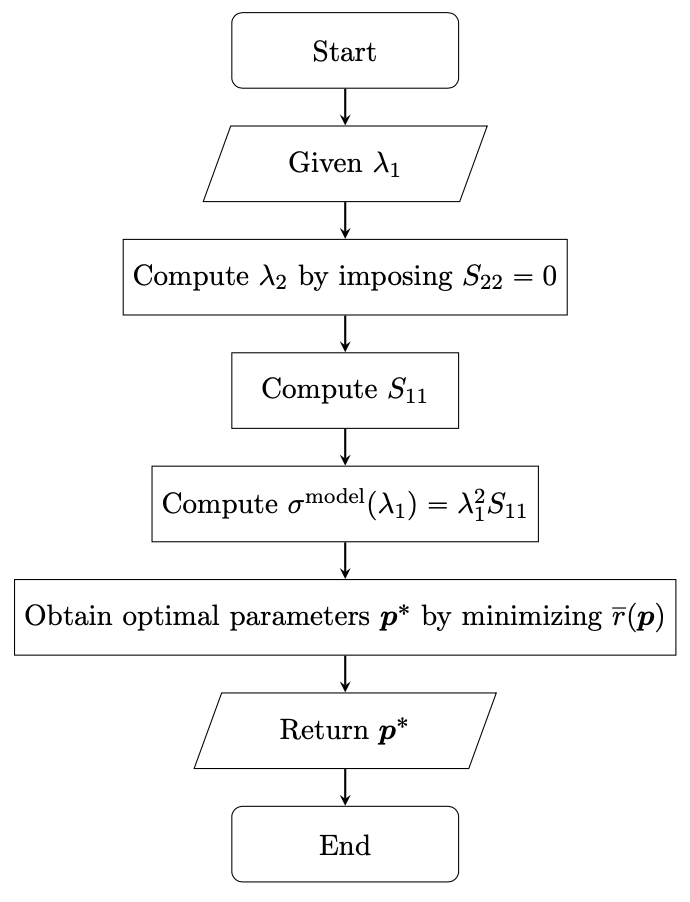
\includegraphics[width = 0.4\textwidth]{Flowchart.png}
    \end{center}
    \caption[Summary of the deterministic calibration.]{Summary of the procedure enabling the deterministic calibration of material parameters on the synthesized samples.}
    \label{fig:flowchart}
\end{figure}
Notice that the optimal values for the parameters involved in the stochastic formulation, gathered in a realization vector $\bfz^*$, are then obtained by using the changes of variables defined in Section \ref{Stochastic Model Homogeneous}.

The results of the adjusted material model and the digitally-generated data for the three layers are shown in Figs.~\ref{fig:det-fit-adv}, \ref{fig:det-fit-med}, and \ref{fig:det-fit-int}. 
\begin{figure}[ht!]
    \begin{center}
        \includegraphics[width = 0.48\textwidth]{Adv_Circ.pdf} \includegraphics[width = 0.48\textwidth]{Adv_Long.pdf}
    \end{center}
    \caption[Fitting results for the adventitia layer.]{Fitting results for the adventitia layer. The reference results are shown in solid black line, while the results obtained with the proposed model are shown in red solid line. Left panel: circumferential direction. Right panel: longitudinal direction.}
    \label{fig:det-fit-adv}
\end{figure}
\begin{figure}[ht!]
    \begin{center}
        \includegraphics[width = 0.48\textwidth]{Med_Circ.pdf} \includegraphics[width = 0.48\textwidth]{Med_Long.pdf}
    \end{center}
    \caption[Fitting results for the media layer.]{Fitting results for the media layer. The reference results are shown in solid black line, while the results obtained with the proposed model are shown in red solid line. Left panel: circumferential direction. Right panel: longitudinal direction.}
    \label{fig:det-fit-med}
\end{figure}
\begin{figure}[ht!]
    \begin{center}
        \includegraphics[width = 0.48\textwidth]{Int_Circ.pdf} \includegraphics[width = 0.48\textwidth]{Int_Long.pdf}
    \end{center}
    \caption[Fitting results for the intima layer.]{Fitting results for the intima layer. The reference results are shown in solid black line, while the results obtained with the proposed model are shown in red solid line. Left panel: circumferential direction. Right panel: longitudinal direction.}
    \label{fig:det-fit-int}
\end{figure}
It is seen that the model can reproduce the data very well, as expected given the similarities between the strain energy density functions used in this paper and in the reference work \cite{holzapfel2005determination} (which only differs in the isotropic contribution). The lists of material parameters thus obtained are provided for all layers in Table~\ref{tab:cal-par-det-adv}, \ref{tab:cal-par-det-med}, and \ref{tab:cal-par-det-int}. The mean averages for these parameters (in the order $\mu_1$, $\mu_2$, $\mu_4$, $\beta_4$, $\alpha$, and $\rho$) are provided for each layer below:
\begin{itemize}
    \item Adventitia: 6.5462 [kPa], 0.1034 [kPa], 21.3557 [kPa], 96.6721 [--], 1.1419 [rad], 0.5151 [--];
    \item Media: 1.2079 [kPa], 0.0230 [kPa], 10.7838 [kPa], 8.1899 [--], 0.3558 [rad], 0.2490 [--];
    \item Intima: 28.4956 [kPa], 0.4725 [kPa], 145.8811 [kPa], 177.3867 [--], 1.1096 [rad], 0.5044 [--].
\end{itemize}

\begin{table}[ht!]
\caption[Calibrated parameters for the adventitia layer.]{Calibrated parameters for the adventitia layer. Specimens numbers are associated with the results presented in \cite{holzapfel2005determination}. Note that the parameter $\mu_4$ here is half of the corresponding parameter in \cite{holzapfel2005determination}, given the expression for the strain energy density function.}
\label{tab:cal-par-det-adv}
\begin{center}
    \begin{tabular}{|c |c| c| c| c| c| c| c|} 
 \hline
 \quad Specimen \quad & \quad $\mu_1$ \quad & \quad $\mu_2$ \quad & \quad $\mu_4$ \quad & \quad $\beta_4$ \quad & \quad $\alpha$ \quad & \quad $\rho$ \quad & Error $\overline{r}(\bfp^*)$ \quad \\
 \quad \# \quad & [kPa] \quad & \quad [kPa] \quad & \quad [kPa] \quad & \quad [--] \quad & \quad [rad] \quad & \quad [--] \quad & $\times 10^{-6}$ \quad \\
 \cline{1-8} 
    1 & 3.8154 & 0.0952   & 16.2516  & 103.8667 & 1.2681 & 0.6503 & 0.3131\\
    2 & 2.2703 & 0.0471   & 6.9480  & 81.3985 & 1.1781 & 0.7510 & 0.8667\\
    3 & 4.8053 & 0.0395   & 33.6126 & 49.4776 & 1.0699 & 0.4999 & 0.1708\\
    5 & 9.1153 & 0.2103   & 41.0040 & 145.0781 & 0.9320 & 0.3998 & 0.8243\\
    6 & 7.7952 & 0.0571   & 12.6815 & 67.9862 & 1.2264 & 0.7003 & 0.1121\\
    8 & 2.0467 & 0.0833   & 18.8116 & 48.7029 & 1.1422 & 0.4040 & 0.2818 \\
    9 & 5.6493 & 0.2089   & 16.4234 & 167.2432 & 1.3151 & 0.2998 & 0.2761\\
    10 & 14.7392 & 0.0778 & 59.5418 & 214.0337 & 0.9320 & 0.6001 & 0.2067\\
    11 & 12.3502 & 0.1629 & 17.5735 & 84.9840 & 1.2083 & 0.6005 & 0.2450\\
    12 & 2.8631 & 0.1009  & 8.7606 & 68.4434 & 0.9597 & 0.4105 & 0.9009\\
    13 & 6.5583 & 0.0541  &  3.3039 & 32.1794 & 1.3297 & 0.3500 & 0.2420\\
 \hline 
\end{tabular}
\end{center}
\end{table}

\begin{table}[ht!]
\caption[Calibrated parameters for the media layer.]{Calibrated parameters for the media layer. Specimens numbers are associated with the results presented in \cite{holzapfel2005determination}. Note that the parameter $\mu_4$ here is half of the corresponding parameter in \cite{holzapfel2005determination}, given the expression for the strain energy density function.}
\label{tab:cal-par-det-med}
\begin{center}
    \begin{tabular}{|c |c| c| c| c| c| c| c|} 
 \hline
 \quad Specimen \quad & \quad $\mu_1$ \quad & \quad $\mu_2$ \quad & \quad $\mu_4$ \quad & \quad $\beta_4$ \quad & \quad $\alpha$ \quad & \quad $\rho$ \quad & Error $\overline{r}(\bfp^*)$ \quad \\
 \quad \# \quad & [kPa] \quad & \quad [kPa] \quad & \quad [kPa] \quad & \quad [--] \quad & \quad [rad] \quad & \quad [--] \quad & $\times 10^{-6}$ \quad \\
 \cline{1-8}
    1 & 0.9122 & 0.0094  & 6.6063  & 10.7580 & 0.3592 & 0.2476 & 0.2793\\
    2 & 1.0174 & 0.0269  & 12.8334  & 5.8988 & 0.4449 & 0.2970 & 0.2268\\
    3 & 1.7214 & 0.0236  & 10.4581  & 5.7353 & 0.3916 & 0.1967 & 0.2478\\
    4 & 1.5992 & 0.0109  &  13.1523 & 9.5337 & 0.4439 & 0.3980 & 0.1677\\
    5 & 2.4868 & 0.0223  & 8.3441  & 13.8411 & 0.2968 & 0.2000 & 0.2959\\
    6 & 0.6409 & 0.0338  & 15.2760  & 5.3399 & 0.3226 & 0.2987 & 0.2007\\
    7 & 0.8698 & 0.0246  & 12.4674  & 7.5124 & 0.2147 & 0.1500 & 0.2853\\
    8 & 0.2368 & 0.0313  &  13.9616 & 5.4142 & 0.1840 & 0.1993 & 0.1661\\
    9 & 2.2856 & 0.0119  &  4.2552  & 12.8970 & 0.4405 & 0.3032 & 0.1334\\
    10 & 0.7071 & 0.0531 & 15.5753 & 2.5561 & 0.2740 & 0.0986 & 0.1921\\
    11 & 1.1838 & 0.0117 & 6.5073 & 8.4201 & 0.5203 & 0.3015 & 0.3128\\
    12 & 0.8871 & 0.0263 & 10.7400 & 7.7343 & 0.3482 & 0.1480 & 0.2638\\
    13 & 1.1550 & 0.0130 & 10.0128 & 10.8277 & 0.3842 & 0.3984 & 0.2561\\
 \hline
\end{tabular}
\end{center}
\end{table}

\begin{table}[ht!]
\caption[Calibrated parameters for the intima layer.]{Calibrated parameters for the intima layer. Specimens numbers are associated with the results presented in \cite{holzapfel2005determination}. Note that the parameter $\mu_4$ here is half of the corresponding parameter in \cite{holzapfel2005determination}, given the expression for the strain energy density function.}
\label{tab:cal-par-det-int}
\begin{center}
    \begin{tabular}{|c |c| c| c| c| c| c| c|} 
 \hline
 \quad Specimen \quad & \quad $\mu_1$ \quad & \quad $\mu_2$ \quad & \quad $\mu_4$ \quad & \quad $\beta_4$ \quad & \quad $\alpha$ \quad & \quad $\rho$ \quad & Error $\overline{r}(\bfp^*)$ \quad \\
 \quad \# \quad & [kPa] \quad & \quad [kPa] \quad & \quad [kPa] \quad & \quad [--] \quad & \quad [rad] \quad & \quad [--] \quad & $\times 10^{-6}$ \quad \\
 \cline{1-8} 
   1 & 26.0930 &   1.0707 &  61.8350 & 180.6829  &  1.2129 &   0.5496 &  0.1064\\
   2 & 42.0952 &   0.1300 & 132.1545 & 286.9763  &  0.9372  &  0.6999 & 0.0253\\
   3 & 24.8050 &   0.2085 & 117.1730 & 176.7649  &  1.0085  &  0.5005 & 0.0233\\
   4 & 48.1296 &   2.2548 & 930.3108 & 454.7669  &  0.8168  &  0.3994 & 0.0235\\
   5 & 24.2734 &   0.1897 & 184.8636 & 342.9503  &  0.6965  &  0.7002 & 0.0266\\
   7 & 34.2402 &   0.1682  & 27.4200 &  92.7600  &  1.2620  &  0.3498 & 0.0307\\
   8 & 25.8023 &   0.1473  & 30.0657 & 110.3671  &  1.2950  &  0.3499 & 0.0253\\
   10 & 27.2055 &   0.1071 &  16.2175 &  72.3563  &  1.1521  &  0.3998 & 0.0223\\
   11 & 25.8057 &   0.1510 &  28.1253  & 77.8412  &  1.1570  &  0.4999 & 0.0256\\
   12 & 15.2380 &   0.5128 &  40.1371 &  73.7906  &  1.3643  &  0.6499 & 0.0203\\
   13 & 19.7643 &   0.2577 &   36.3891 &  81.9973 &   1.3036  &  0.4498 & 0.0263\\
 \hline 
\end{tabular}
\end{center}
\end{table}


\subsection{Calibration of the Stochastic Model} \label{subsec:sto-calibration}

Since the components of $\bfZ$ are statistically independent, we use the maximum likelihood method to calibrate the hyperparameters for each random variable. Denote by $\boldsymbol{s}$ the vector gathering the set of hyperparameters for a given component of $\bfZ$ in the stochastic model. The optimal value of $\boldsymbol{s}$ is then obtained as
\begin{align}
    \hat{\boldsymbol{s}} &= \text{argmax}_{\boldsymbol{s} \in \mathcal{C}_{\boldsymbol{s}}} \quad \mathcal{L}(\boldsymbol{s}; \bfy)\,,
\end{align}
where $\mathcal{C}_{\boldsymbol{s}}$ denotes the parameter space, $\mathcal{L}$ is the likelihood function, and $\bfy$ is the observed data sample. The values of all hyperparameters are given in Table~\ref{tab:hyperparameters}, and the associated probability density functions (together with samples) are shown in Figs.~\ref{fig:MLE-Set-1}, \ref{fig:MLE-Set-2}, and \ref{fig:MLE-Set-3}.
\begin{table}[ht!]
\caption[Hyperparameters estimated with the maximum likelihood method.]{Hyperparameters estimated with the maximum likelihood method for all layers.}
\label{tab:hyperparameters}
\begin{center}
    \begin{tabular}{|c|c|c|c|} 
 \hline
 \quad Parameter \quad & \quad $\hat{\boldsymbol{s}}$ (adventitia) \quad & \quad $\hat{\boldsymbol{s}}$ (media) \quad & \quad $\hat{\boldsymbol{s}}$ (intima) \quad \\
 \cline{1-4} 
    $C_2$ & $(2.9459, 4.6266)$  & $(3.6841, 0.7075)$   & $(1.4120, 35.8575)$\\
    $V$   & $(1.6574, 99.5985)$ & $(5.9044, 22.4244)$  & $(0.6364, 1.645 \times 10^3)$\\
    $B_4$ & $(3.5262, 27.4153)$ & $(5.2736, 1.5154)$   & $(1.1744, 129.0230)$\\
    $U$   & $(48.4729, 2.5140)$ & $(14.4793, 1.1649)$  & $(34.4290, 1.43553)$\\
    $R$   & $(5.8703, 5.5101)$  & $(6.25578, 19.3627)$ & $(3.1868, 1.9178)$\\
    $T$   & $(17.7955, 6.6881)$ & $(8.8830, 30.5876)$  & $(4.5830, 5.2297)$\\
 \hline 
\end{tabular}
\end{center}
\end{table}
In practice, these hyperparameters can used to generate mathematically-consistent virtual samples. 

\begin{figure}[ht!]
    \begin{center}
        \includegraphics[width = 0.48\textwidth]{MLE-C2.pdf} \includegraphics[width = 0.48\textwidth]{MLE-V.pdf}
    \end{center}
    \caption[Probability density functions (PDFs) of $C_2$ and $V$.]{Probability density functions (PDFs), with hyperparameters estimated with the maximum likelihood method, and experimental samples. Left panel: random variable $C_2$. Right panel: random variable $V$.}
    \label{fig:MLE-Set-1}
\end{figure}
\begin{figure}[ht!]
    \begin{center}
        \includegraphics[width = 0.48\textwidth]{MLE-B4.pdf} \includegraphics[width = 0.48\textwidth]{MLE-U.pdf}
    \end{center}
    \caption[Probability density functions (PDFs) of $B_2$ and $U$.]{Probability density functions (PDFs), with hyperparameters estimated with the maximum likelihood method, and experimental samples. Left panel: random variable $B_2$. Right panel: random variable $U$.}
    \label{fig:MLE-Set-2}
\end{figure}
\begin{figure}[ht!]
    \begin{center}
        \includegraphics[width = 0.48\textwidth]{MLE-T.pdf} \includegraphics[width = 0.48\textwidth]{MLE-R.pdf}
    \end{center}
    \caption[Probability density functions (PDFs) of $T$ and $R$.]{Probability density functions (PDFs), with hyperparameters estimated with the maximum likelihood method, and experimental samples. Left panel: random variable $T$. Right panel: random variable $R$.}
    \label{fig:MLE-Set-3}
\end{figure}

Using these results, new samples of $\bfZ$ can be generated and pulled back to obtain samples of the primary parameters defining the strain energy density function. Using $10^{6}$ samples, the following mean values were obtained for these parameters:
\begin{itemize}
    \item Adventitia: 6.4760 [kPa], 0.1297 [kPa], 24.0164 [kPa], 96.4960 [--], 1.1426 [rad], 0.5172 [--];
    \item Media: 1.2076 [kPa], 0.0379 [kPa], 11.1438 [kPa], 8.0084 [--], 0.3539 [rad], 0.2440 [--];
    \item Intima: 24.2965 [kPa], 0.3893 [kPa], 136.2482 [kPa], 151.3538 [--], 0.9806 [rad], 0.4672 [--].
\end{itemize}
It is seen that these results slightly differ from the ones reported in Section \ref{subsec:det-calibration}, where mean averaging was used instead of a maximum likelihood estimator. In order to qualitatively assess this result, the mean responses obtained by using either parameterization (that is, the one provided in Section \ref{subsec:det-calibration} or the one given above) are shown for all layers and both directions in Figs.~\ref{fig:mean-adv}, \ref{fig:mean-med}, and \ref{fig:mean-int}. The difference between the two responses is most noticeable for the intima layer, due to the strong stiffening effect. Finally, 95\% confidence intervals were estimated with the model, using 100,000 independent samples. These intervals are also displayed in Figs.~\ref{fig:mean-adv}, \ref{fig:mean-med}, and \ref{fig:mean-int}, and are seen to capture experimental variability with reasonable accuracy.
\begin{figure}[ht!]
    \begin{center}
        \includegraphics[width = 0.48\textwidth]{MeanCI-Adv-Circ.pdf} \includegraphics[width = 0.48\textwidth]{MeanCI-Adv-Long.pdf}
    \end{center}
    \caption[Experimental results obtained for the adventitia layer.]{Experimental results (black solid lines), mean responses obtained for the adventitia layer by using either the MLE-based estimate (blue solid line) or a mean average (blue dashed line), and 95\% confidence interval (red solid line). Left panel: circumferential direction. Right panel: longitudinal direction.}
    \label{fig:mean-adv}
\end{figure}
\begin{figure}[ht!]
    \begin{center}
        \includegraphics[width = 0.48\textwidth]{MeanCI-Med-Circ.pdf} \includegraphics[width = 0.48\textwidth]{MeanCI-Med-Long.pdf}
    \end{center}
    \caption[Experimental results obtained for the media layer.]{Experimental results (black solid lines), mean responses obtained for the media layer by using either the MLE-based estimate (blue solid line) or a mean average (blue dashed line), and 95\% confidence interval (red solid line). Left panel: circumferential direction. Right panel: longitudinal direction.}
    \label{fig:mean-med}
\end{figure}
\begin{figure}[ht!]
    \begin{center}
        \includegraphics[width = 0.48\textwidth]{MeanCI-Int-Circ.pdf} \includegraphics[width = 0.48\textwidth]{MeanCI-Int-Long.pdf}
    \end{center}
    \caption[Experimental results obtained for the intima layer.]{Experimental results (black solid lines), mean responses obtained for the intima layer by using either the MLE-based estimate (blue solid line) or a mean average (blue dashed line), and 95\% confidence interval (red solid line). Left panel: circumferential direction. Right panel: longitudinal direction.}
    \label{fig:mean-int}
\end{figure}

\section{Uncertainty Propagation} \label{sec:uncertainty-propagation}


\subsection{Definition of the Random Field Model on a Patient-Specific Geometry}

In this section, we consider the propagation of the uncertainties associated with the proposed random field model on a patient-specific geometry. Without loss of generality, we assume that the latter corresponds to the adventitia layer (which is the outermost layer in the arterial wall). We use the domain studied in \cite{STABER201894}, which was obtained by postprocessing the inner surface available as file 0098 in the Aneurisk database \cite{AneuriskWeb}. The domain is about $12$ [mm] long and is shown in Fig.~\ref{fig:geometry}. Details about discretization are provided in Section \ref{subsec:SFEM-propagation}.
\begin{figure}[ht!]
    \begin{center}
        \includegraphics[trim = {5cm 7cm 5cm 7cm}, clip, width = 0.48\textwidth]{Artery3D.pdf} \includegraphics[trim = {5cm 5cm 5cm 7cm}, clip, width = 0.4\textwidth]{ArterySlice.pdf}
    \end{center}
    \caption[Three-dimensional and slice views of the arterial wall.]{Three-dimensional and slice views of the arterial wall, computed from \cite{AneuriskWeb}.}
    \label{fig:geometry}
\end{figure}

In order to define the latent Gaussian field $\{{\bf \Xi}(\bfx), \bfx \in B\}$, we use the SPDE approach introduced in Section \ref{subsec:def-Gaussian} (with $\alpha = 2$). As a preliminary step, we use the Laplace-Dirichlet Rule-Based algorithm \cite{Bayer2012,Augustin2014} to define some local orientation fields involved in the parameterization of the diffusion $[H]$. Specifically, we introduce the vector fields $\bfx \mapsto \bfe^{(1)}(\bfx)$ and $\bfx \mapsto \bfe^{(2)}(\bfx)$ defined as
\begin{equation}
\bs{e}^{(1)}(\bs{x}) = \frac{\nabla\Psi_2(\bs{x})}{ \| \nabla \Psi_2(\bs{x}) \| }~, \quad \bs{e}^{(2)}(\bs{x}) = \bs{e}^{(3)}(\bs{x}) \times \bs{e}^{(1)}(\bs{x})~, \quad \bs{e}^{(3)}(\bs{x}) = \frac{\nabla \Psi_1(\bs{x})}{ \| \nabla \Psi_1(\bs{x}) \| }~,
\end{equation}
where $\bs{x} \mapsto \Psi_1(\bs{x})$ satisfies 
\begin{equation}
\Delta \Psi_1({\bs{x}}) = 0~, \quad \forall \, {\bs{x}} \in B~,
\end{equation}
with $\Psi_1({\bs{x}}) = 0$ on the inlet surface and $\Psi_1({\bs{x}}) = 1$ on the outlet surface, and $\bs{x} \mapsto \Psi_2(\bs{x})$ is the solution to a similar Laplace problem with $\Psi_2({\bs{x}}) = 0$ on the inner surface and $\Psi_2({\bs{x}}) = 1$ on the outer surface \cite{STABER201894}.

As a first step, we then consider the Gaussian component associated with the angle random field $\{A(\bfx), \bfx \in B\}$ and use a SPDE where the diffusion field is defined as
\begin{equation}\label{eq:def-H-final-application}
    \bs{D}(\bfx) = \kappa \bs{I} + \tau_1 \hat{\bfe}^{(1)}(\bfx) \otimes \hat{\bfe}^{(1)}(\bfx) + \tau_2 \hat{\bfe}^{(2)}(\bfx) \otimes \hat{\bfe}^{(2)}(\bfx)\,,
\end{equation}
where
\begin{equation}    
    \hat{\bfe}^{(1)}(\bfx) = \cos(\underline{a}) \bfe^{(1)}(\bfx) + \sin(\underline{a})\bfe^{(2)}(\bfx)\,, \quad \hat{\bfe}^{(2)}(\bfx) = \cos(\underline{a}) \bfe^{(1)}(\bfx) - \sin(\underline{a})\bfe^{(2)}(\bfx)\,,
\end{equation}
and $\underline{a}$ is the mean value for the angle obtained from the calibrated step detailed in Section \ref{sec:calibration} (for the adventitia layer). In effect, this introduces some waviness effect in the local orientation, for both the anisotropic mechanical behavior and covariance structure, which can be related to waviness in the orientation of collagen fibers at a finer scale. By construction, this modeling feature can be turned off by setting the associated coefficient of variation to zero.

Next, and for a \textit{given} sample $\bfx \mapsto a(\bfx, \theta)$ of the angle random field thus obtained, with $\theta \in \Theta$, the latent Gaussian components associated with the other material random fields are defined and sampled by solving the SPDE with the diffusion taken as in Eq.~\eqref{eq:def-H-final-application}, where the orientation vectors are now defined as
\begin{equation}    
    \hat{\bfe}^{(1)}(\bfx) = \cos(a(\bfx, \theta)) \bfe^{(1)}(\bfx) + \sin(a(\bfx, \theta))\bfe^{(2)}(\bfx)
\end{equation}
and
\begin{equation}    
 \hat{\bfe}^{(2)}(\bfx) = \cos(a(\bfx, \theta)) \bfe^{(1)}(\bfx) - \sin(a(\bfx, \theta))\bfe^{(2)}(\bfx)\,.
\end{equation}

Following the methodology of construction presented in Section \ref{sec:sto-heterogeneous}, we now proceed with the specification of the hyperparameters defining the transport map $H$. A natural choice here is to use the parameters identified in Section \ref{subsec:sto-calibration}; see Table~\ref{tab:hyperparameters}. However, the associated probability density functions represent inter-patient variability and would therefore generate unrealistically large (intra-patient) spatial fluctuations. For this reason, we propose to preserve the mean values estimated at the calibration stage, and to scale the coefficients of variation in a proportional manner (meaning that properties that exhibit larger fluctuations still present larger spatial variations). The proposed values for these coefficients of variation are listed in Table~\ref{tab:scaled-hyperparameters}.
\begin{table}[ht!]
\caption[Scaled coefficients of variation of the random variables.]{Scaled values for the coefficients of variation of the random variables.}
\label{tab:scaled-hyperparameters}
\begin{center}
    \begin{tabular}{|c|c|c|} 
 \hline
 \quad Parameter \quad & \quad Data-based coefficient of variation \quad & \quad Scaled coefficient of variation \quad \\
 \cline{1-3} 
    $C_2$ & $0.5826$  & $0.15$ \\
    $V$   & $0.7768$ & $0.2$ \\
    $B_4$ & $0.5325$ & $0.1371$ \\
    $U$   & $0.0316$ & $0.0081$ \\
    $R$   & $0.2753$  & $0.0709$ \\
    $T$   & $0.1214$ & $0.0313$ \\
 \hline 
 \end{tabular}
\end{center}
\end{table}
The corresponding set of hyperparameters are provided in Table~\ref{tab:hyperparameters-scaled}.
\begin{table}[ht!]
\caption[Hyperparameters corresponding to the scaled coefficients of variation.]{Hyperparameters corresponding to the scaled coefficients of variation (given in the far-right column in Table~\ref{tab:scaled-hyperparameters}).}
\label{tab:hyperparameters-scaled}
\begin{center}
    \begin{tabular}{|c|c|} 
 \hline
 \quad Parameter \quad & \quad $\hat{\boldsymbol{s}}$ (adventitia) \quad \\
 \cline{1-2} 
    $C_2$ & $(44.4351, 0.3067)$\\
    $V$   & $(25, 6.6031)$\\
    $B_4$ & $(53.1877, 1.8176)$\\
    $U$   & $(744.5323, 38.6146)$\\
    $R$   & $(95.81, 89.9306)$\\
    $T$   & $(278.6547, 104.727)$\\
 \hline 
\end{tabular}
\end{center}
\end{table}

Realizations of the random fields of material parameters are shown in Figs.~\ref{fig:samples-1}, \ref{fig:samples-2}, and \ref{fig:samples-3}, for $\gamma = 1$, $\kappa = 0.1$, and $\tau_1 = \tau_2 = 10$. These values are selected for the sake of illustration to induce moderate correlation ranges on the arterial wall. The identification of such parameters requires spatial data that are not currently available for the proposed application (and may be obtained using, e.g., ultrasound characterization techniques) and is left for future work.
\begin{figure}[ht!]
    \begin{center}
        
    \includegraphics[trim = {6cm 3cm 6cm 5cm}, clip, width = 0.48\textwidth]{Sample_G1.pdf} \includegraphics[trim = {6cm 3cm 6cm 5cm}, clip, width = 0.48\textwidth]{Sample_G2.pdf}
    \end{center}
    \caption[Sample of $\{G_1(\bfx), \bfx \in B\}$ and $\{G_2(\bfx), \bfx \in B\}$ in the adventitia layer.]{Sample of $\{G_1(\bfx), \bfx \in B\}$ (left) and $\{G_2(\bfx), \bfx \in B\}$ (right) in the adventitia layer.}
    \label{fig:samples-1}
\end{figure}

\begin{figure}[ht!]
    \begin{center}
        \includegraphics[trim = {6cm 3cm 6cm 5cm}, clip, width = 0.48\textwidth]{Sample_G4.pdf} \includegraphics[trim = {6cm 3cm 6cm 5cm}, clip, width = 0.48\textwidth]{Sample_B4.pdf}
    \end{center}
    \caption[Sample of $\{G_4(\bfx), \bfx \in B\}$ and $\{B_4(\bfx), \bfx \in B\}$ in the adventitia layer.]{Sample of $\{G_4(\bfx), \bfx \in B\}$ (left) and $\{B_4(\bfx), \bfx \in B\}$ (right) in the adventitia layer.}
    \label{fig:samples-2}
\end{figure}

\begin{figure}[ht!]
    \begin{center}
        \includegraphics[trim = {6cm 3cm 6cm 5cm}, clip, width = 0.48\textwidth]{Sample_R.pdf} \includegraphics[trim = {6cm 3cm 6cm 5cm}, clip, width = 0.48\textwidth]{Sample_A.pdf}
    \end{center}
    \caption[Sample of $\{R(\bfx), \bfx \in B\}$ and $\{A(\bfx), \bfx \in B\}$ in the adventitia layer.]{Sample of $\{R(\bfx), \bfx \in B\}$ (left) and $\{A(\bfx), \bfx \in B\}$ (right) in the adventitia layer.}
    \label{fig:samples-3}
\end{figure}

\subsection{Propagation of Uncertainties}\label{subsec:SFEM-propagation}

In this work, the nonlinear boundary value problem is solved by the finite element method, using a total Lagrangian formulation and a three-field formulation ($\mathbb{P}_2$-$\mathbb{P}_0$-$\mathbb{P}_0$ discretization) to handle quasi-incompressibility \cite{wriggers2008nonlinear}. The geometry shown in Fig.~\ref{fig:geometry} is discretized with a mesh containing $297,828$ cells and $432,250$ nodes. An inflating pressure of 1 [kPa] is applied on the inner layer and sliding displacement boundary conditions are prescribed on the inlet and outlet surfaces (the system is made statically determined by restricting additional degrees of freedom at two nodes located on the outlet surface). Implementation was performed within the MOOSE finite element framework \cite{permann2020moose} and code verification was conducted through the method of manufactured solution (described in \ref{app:VV-artery}).  

Given the random field modeling setting, a Monte-Carlo approach was used to propagate uncertainties (see the remark at the end of this section). Interested readers are referred to \cite{Ghanem2017} for a comprehensive review on alternative stochastic solvers (see \cite{hauseux2018quantifying} for a specific discussion regarding hyperelastic materials). Parallel computing with 36 cores was used to accelerate the deterministic runs.

The fields of mean values and coefficients of variation are shown in Fig.~\ref{fig:vonMises}.
\begin{figure}[ht!]
    \begin{center}
        \includegraphics[trim = {6cm 3cm 6cm 5cm}, clip, width = 0.48\textwidth]{Mean-vMStress.pdf} \includegraphics[trim = {6cm 3cm 6cm 5cm}, clip, width = 0.48\textwidth]{CV-vMStress.pdf}
    \end{center}
    \caption[Mean and coefficient of variation for the von Mises stress.]{Mean (left) and coefficient of variation (right) for the von Mises stress (slice views).}
    \label{fig:vonMises}
\end{figure}
Substantial spatial variations are observed in both fields and localization is less pronounced than in the results presented in \cite{STABER201894}---as angular waviness tends to mitigate that effect. Values for the mean field range from 0.15 to 40 [kPa], while values for the coefficient of variation are distributed between 0.025 to 0.42. While these quantitative results are conditioned by the proposed scaling in variance (defined in Tab.~\ref{tab:scaled-hyperparameters}) and the selected values for the hyperparameters defining the latent Gaussian fields, they show the impact of material variability on the response of the arterial wall. Additional work assimilating spatial data is therefore necessary to refine the propagation analysis and translate the results into practical applications: the proposed modeling framework is a first step towards that goal.

\begin{remark}
The usual spectral approach to uncertainty propagation consists in representing the random fields through Karhunen-Lo\`eve expansions and in seeking a polynomial chaos surrogate in terms of the reduced variables. It is therefore instructive to analyze a posteriori the dimension obtained for a given field defined and sampled through the SPDE approach, say $\{G_1(\bfx), \bfx \in B\}$. The graph of the standard error function $n \mapsto \textnormal{Conv}(n)$, where
\begin{equation}
    \textnormal{Conv}(n) = 1 - \frac{\sum_{i = 1}^{n} \lambda_i}{\textnormal{tr}(\textnormal{Cov}\{G_1\})}
\end{equation}
and the covariance matrix $\textnormal{Cov}\{G_1\}$ (and its eigenvalues $\{\lambda_i\}_{i \geq 1}$) are computed by using a singular value decomposition on the matrix of centered samples (200 samples are used here), is shown in Fig.~\ref{fig:conv}.
\begin{figure}[ht!]
    \begin{center}
        \includegraphics[width = 0.5\textwidth]{ConvN.pdf}
    \end{center}
    \caption[Graph of the function $n \mapsto \textnormal{Conv}(n)$.]{Graph of the function $n \mapsto \textnormal{Conv}(n)$.}
    \label{fig:conv}
\end{figure}
Retaining a truncation threshold of $0.01$ leads to a reduced dimension of 158, which suggests---given that six random fields are involved in the parameterization of the stochastic strain energy density function---a very high-dimensional setting for propagation through collocation-type approaches.
\end{remark} % A regular chapter, starts with '\chapter{Title}'
\chapter{Polyconvex Neural Networks for Hyperelastic Constitutive Models: A Rectification Approach}
\label{chap:polyconvex}

Constitutive models based on neural networks (NN) have received growing attention over the past few years, owing to their ability to represent nonlinear mappings in a high dimensional setting. There is a very substantial amount of papers published on this topic, for a wide variety of material behaviors; see, \textit{e.g.},  \cite{flaschel2021unsupervised,xu2021learning,holzapfel2021predictive,jung2006neural,ghaboussi1998autoprogressive,ghaboussi1998new,hashash2004numerical,furukawa1998implicit,joshi2022bayesian,as2022mechanics,Asad-IJNME,KLEIN2022104703} and the references therein, in a non-exhaustive manner.

Beyond classical data science aspects that pertain to architecture design, training and validation strategies, and the analysis of approximation capabilities, a central concern is to make such surrogates amenable to scientific simulations where such models are typically set to parameterize systems of partial differential equations. In this context, the surrogate must satisfy both physical assumptions and mathematical properties (\textit{e.g.}, boundedness or a certain type of convexity) to ensure the existence (and potentially, the uniqueness) of solutions. 
In the case of nonlinear elasticity for instance, a strain energy density function is theoretically required to satisfy frame indifference, some asymptotic behavior, and specific convexity and growth conditions. There are various ways to enforce such properties and in particular, the convexity requirement. The simplest strategy consists in using some unconstrained neural network that, if properly calibrated on a rich enough dataset, may possess desired convexity. Another way to enforce convexity is to add a penalty term in the loss function during the training stage; see, \textit{e.g.}, \cite{liu2020generic}. This latter strategy corresponds to a weak enforcement and hence does not prevent from checking the condition \textit{a posteriori}. 

In this work, we consider enforcing convexity in the strong sense, by defining classes of surrogate models that satisfy the condition \textit{a priori}. The issue of ensuring the convexity of a neural network is not new and was mostly tackled by constraining the network through the use of non-negative weights and convex activation functions \cite{amos2017input}. Restriction on weights can be imposed by constraining the weights during training, or by using a mapping from $\mathbb{R}$ into $\mathbb{R}_{\geq 0}$ that acts on unconstrained weights \cite{sivaprasad2021curious,Asad-IJNME}. Applications in computational mechanics are presented in \cite{masi2021thermodynamics, as2022mechanics,Asad-IJNME} for example. A detailed analysis about the use of constrained neural networks for polyconvex anisotropic hyperelastic models can be found in \cite{KLEIN2022104703}, in particular.

Here, we aim to construct a convex neural network model without affecting expressiveness (that is, without constraining weights \textit{a priori}) and training cost (which can be affected by transformations performed on weights at the training stage). Building upon recent works on monotonic neural networks \cite{wehenkel2019unconstrained} and monotone transport maps for density estimation \cite{baptista2020adaptive}, our approach relies on simple integral representations to define an operator that transforms any arbitrary function (and in particular, a \textit{free} neural network) into a convex function. This strategy thus entails the rectification of the whole neural network model. We show, through various numerical experiments on both digitally synthesized and experimental datasets, that the proposed rectified models enable proper fitting. They are also seen to converge much faster than constrained models (in terms of number of iterations)---at the expense of an increased computational cost per iteration. 

The rest of this section is organized as follows. The mechanistic parameterization and rectification strategy are first presented in Section~\ref{sec:rectifiers} (together with a toy example). Applications to standard hyperelastic models relevant to both isotropic and anisotropic materials are then discussed in Section \ref{sec:applications}.

\section{Rectified Neural Network Representations}
\label{sec:rectifiers}

\subsection{Background in Elasticity}
Let $\Omega$ be a collection of material points identified with their vector of coordinates $\bfX$ in $\mathbb{R}^3$, and denote by $\partial \Omega$ the boundary of $\Omega$. For any material point $\bfX \in \Omega$, the spatial point $\bfx$ in the deformed configuration $\Omega^\varphi$ is given by $\bfx = \varphi (\bfX)$, where $\varphi$ is the deformation map. For any $\bfX \in \Omega$, the deformation gradient $\defgrad$ is a second-order tensor defined as $\defgrad = \grad_{\bfX} \bfx$. The left and right Cauchy-Green deformation tensors are given by $\bfB = \defgrad \defgrad^T$ and $\rcg = \defgrad^T \defgrad$, respectively.

We seek to construct a neural network surrogate that satisfies physical axioms and mathematical requirements arising in existence theorem in finite elasticity. From a theoretical standpoint, strain energy density functions are required to satisfy \cite{ciarlet1988mathematical,truesdell2004non}:
\begin{enumerate}
    \item Principle of material frame indifference (objectivity), stated as: $\forall \bfQ \in \mathrm{SO}(3)$,
    \begin{equation}
            w(\bfQ \bfF) = w(\bfF)\,, \quad \bfP(\bfQ \bfF) = \bfQ \bfP(\bfF)\,,
    \end{equation}
    where $\bfP$ is the first Piola-Kirchhoff stress tensor;
    \item Proper convexity conditions; 
    \item Some asymptotic behavior as $\det (\bfF) \to 0^+$; and
    \item A coerciveness inequality (growth conditions).
\end{enumerate}
In particular, the requirements (2--4) are fundamental to ensure the existence of (at least) one minimizer for the energy functional, see Chapter 7 in \cite{ciarlet1988mathematical} (see also \cite{pedregal2000variational,Dacorogna1989}).

Material frame-indifference is, in general, achieved by defining $w$ in terms of the right Cauchy-Green deformation tensor $\bfC$, which is an \textit{a priori} objective kinematic variable \cite{truesdell2004non}. Following the work by Ball \cite{ball1976convexity}, polyconvexity is often imposed in lieu of convexity, as (i) it does not conflict with any physical constraints; (ii) it is generally satisfied by commonly employed models; and (iii) it enables the derivation of powerful existence results \cite{ciarlet1988mathematical}. To proceed with the construction of the model, it is instructive at this point to recall the definition of polyconvexity. A strain energy density function $w:\mathbb{M}_+^3 \to \mathbb{R}$ is polyconvex if there exists a convex function $w^*:\mathbb{M}^3 \times \mathbb{M}^3 \times \mathbb{R}$ such that
\begin{equation}  
    w(\bfF) = w^*(\bfF, \mathrm{Cof}(\bfF), \det(\bfF))\,, 
\end{equation}
for all $\bfF \in \mathbb{M}_+^3$, where (i) $\mathrm{Cof}(\bfF)$ and $\det(\bfF)$ are the cofactor matrix and determinant of $\bfF$; (ii) $\mathbb{M}^3$ and $\mathbb{M}_+^3$ denote the sets of real square matrices of order $3$ with arbitrary and strictly positive determinants, respectively. The requirements (3) and (4) above, related to volume annihilation and coercivity, are crucial in the analytical derivation of functional forms for $w$. They are, however, less relevant to surrogate modeling which only involves bounded intervals, by construction. In this context, the choice of a proper parameterization (in terms of $\bfC$) and the satisfaction of the polyconvexity requirement are sufficient to ensure well-posedness and physical consistency. 

Following the previous discussion, we then consider the construction of a polyconvex surrogate, that is $w(\bfC) = w^*(I_1, I_2, I_3)$
% \begin{equation}
%     w(\bfC) = w^*(I_1, I_2, I_3)
% \end{equation}
owing to a slight abuse of notation, where $I_1 = \tr \bfC$, $I_2 = \tr [ \mathrm{Cof}\,\bfC ]$, and $I_3 = \det \bfC$ are the polyconvex invariants of the right Cauchy-Green tensor $\bfC$. We assume an additive decomposition and define $w^*$ as
\begin{equation}
    w^*(I_1, I_2, I_3) := \sum_{i = 1}^{3} w_i^*(I_i)\,,
\end{equation}
where $\{w_i^*\}_{i = 1}^3$ are convex in the associated variables, hence ensuring the polyconvexity of $w^*$ \cite{hartmann2003polyconvexity,schroder2003invariant}. Notice that the above formulation can readily be extended to model anisotropic behaviors, by including mixed invariants that involve structural tensors \cite{ebbing2010construction} (see Sections \ref{subsec:anisotropic-app} and \ref{subsec:exp-app}). 

Our aim now is to construct the set of convex functions $\{w_i^*\}_{i = 1}^3$ using \textit{fully unconstrained} neural networks. %To that end, we invoke the integral representation for convex functions, as detailed in the next section.

\subsection{Rectification of Unconstrained Neural Networks for Constitutive Modeling in Finite Elasticity}
\label{subsec:rectification}
In order to define the functions $\{w_i^*\}_{i = 1}^3$, we start by recalling the integral representation of convex functions, using generic notation. 

Let $f:I \to \mathbb{R}$ be a convex function. Then $f$ admits the representation
\begin{equation}\label{eq:Rec-Con}
    f(x) = f(a) + \int_a^x \phi(t)\,dt\,,
\end{equation}
for $a < x$ in the interval $I$, where $\phi:I \to \mathbb{R}$ is a nondecreasing function. The constant $f(a)$ in the right-hand side of Eq.~\eqref{eq:Rec-Con} can be derived by fixing the value of $f$ at some point $x^\star \geq a$ in $I$, that is
\begin{equation}\label{eq:Rec-Con-Value}
    f(a) = f(x^\star) - \int_a^{x^\star} \phi(t)\,dt\,.
\end{equation}
In the case of a strain energy density function, the point $x^\star$ is associated with the normalization condition $w(\bfI) = 0$.

The central idea is to define $\phi$ in terms of an arbitrary function, soon to be taken as an unconstrained NN. In order to enforce the monotonicity of $\phi$, we rely on the representation proposed in \cite{baptista2020adaptive} to enforce monotonicity on transport maps. Specifically, we define $\phi$ as
\begin{equation}\label{eq:Rec-Inc}
    \phi(t) := \Phi(0) + \int_{0}^{t} g\left(\frac{d\Phi(z)}{dz}\right)\,dz\,,
\end{equation}
where $\Phi:\mathbb{R} \to \mathbb{R}$ is \textit{any} smooth function and $g:\mathbb{R} \to \mathbb{R}_{\geq 0}$ is a positive function. The operator defined by Eq.~\eqref{eq:Rec-Inc} maps any function $\Phi$ into a non-decreasing function $\phi$ and was called, for this reason, a rectifier in \cite{baptista2020adaptive}. We use this terminology below, and write 
\begin{equation}
    \phi = \mathcal{R}_{\mathrm{inc}}\{\Phi\}\,, \quad \phi(t) = \mathcal{R}_{\mathrm{inc}}\{\Phi\}(t) \, \quad \forall t \in \mathbb{R}\,.
\end{equation}
Similarly, Eq.~\eqref{eq:Rec-Con} can be written as 
\begin{equation}
    f = \mathcal{R}_{\mathrm{cvx}}\{\phi\}\,, \quad f(x) = \mathcal{R}_{\mathrm{cvx}}\{\phi\}(x) \quad \forall x \in I\,,
\end{equation}
where $\mathcal{R}_{\mathrm{cvx}}$ is seen as a second rectifier. Consequently, the convex function $f$ can be defined as
\begin{equation}
    f = \mathcal{R}\{\Phi\}\,, \quad \mathcal{R} := \mathcal{R}_{\mathrm{cvx}} \circ \mathcal{R}_{\mathrm{inc}}\,,
\end{equation}
where the composite rectifier $\mathcal{R}$ implicitly depends on the function $g$. Several choices were proposed and studied in the literature, including the exponential, modified soft-plus, or square functions \cite{baptista2020adaptive}. It follows that each function $w_i^*$, $1 \leq i \leq 3$, can be defined as
\begin{equation}\label{eq:def-wistar}
    w_i^*(I_i) := \mathcal{R}\{\psi_i(\{\bfW_j^{(i)}, \bfb_j^{(i)}\}_{j = 1}^{n_i})\}(I_i)\,, 
\end{equation}
where $\psi_i$ is the \textit{unconstrained} neural network associated with input variable $I_i$, with weights and biases gathered in $\{\bfW_j^{(i)}\}_{j = 1}^{n_i}$ and $\{\bfb_j^{(i)}\}_{j = 1}^{n_i}$, respectively, and $n_i$ is the number of layers (including the hidden and output layers). The neural network $\psi_i$ associated with $I_i$ is written as
\begin{align}
     \psi_i(I_i) := & ~ \bfW_{n_i}^{(i)}(\ldots A_1^{(i)}(\bfW_1^{(i)} I_i + \bfb_1^{(i)}) \ldots) \nonumber \\
     & \quad + \bfb_{n_i}^{(i)}\,,
\end{align}
where $\{A_j^{(i)}\}_{j=1}^{n_i-1}$ are $(n_i-1)$ vector-valued, component-wise acting activation functions (note that no activation function is used for the outer layer). The rectified neural network surrogate for the strain energy function is finally obtained as
\begin{equation}
    w^*(I_1,I_2,I_3) = \sum_{i = 1}^{3} \mathcal{R}\{\psi_i(\{\bfW_j^{(i)}, \bfb_j^{(i)}\}_{j = 1}^{n_i})\}(I_i)\,. 
\end{equation}
While the neural networks $\{\psi_i\}_{i = 1}^3$ are left undefined at this stage, it should be noticed that the architectures must be such that the surrogate $w^*$ is twice differentiable. The integral representation makes this requirement weaker, as the neural network only needs to be differentiable. 
Finally, $w^*$ must satisfy the normalization condition 
\begin{equation}\label{eq:constraint-shift}
    w^*(3, 3, 1) = 0\,,
\end{equation}
as well as the constraint
\begin{equation}\label{eq:constraint-stationarity}
    \left.\frac{\partial w_1^*(I_1)}{\partial I_1}\right\vert_{I_1 = 3} + \left.2\frac{\partial w_2^*(I_2)}{\partial I_2}\right\vert_{I_2 = 3} + \left.\frac{\partial w_3^*(I_3)}{\partial I_3}\right\vert_{I_3 = 1} = 0\,,
\end{equation}
stemming from the stationarity of the (isotropic) strain energy density function at $\bfC = \bfI$. 

Eq.~\eqref{eq:constraint-shift} can be enforced by the shift defined by Eq.~\eqref{eq:Rec-Con-Value}. The constraint given by Eq.~\eqref{eq:constraint-stationarity}  can be accounted for in two ways. Weak enforcement can be achieved by adding a penalty term in the loss function during training. This strategy may, however, lead to spurious behaviors that were reported in \cite{Asad-IJNME} for example. Alternatively, the stress-free constraint may be integrated in the strong sense either by enforcing an algebraic equation on hyperparameters, or by simply shifting the stress value at the origin \cite{Asad-IJNME}. The former approach leads to nonlinear constraints and was found to affect expressiveness in numerical experiments. In contrast, the latter strategy usually enables good accuracy and can easily be implemented. For these reasons, the stress shift strategy will be used in the examples discussed in Section \ref{sec:applications}. Note that this amounts to adding a term in the strain energy density function that does not affect its properties in terms of theoretical requirements (\textit{e.g.}, convexity); see the discussion in \cite{Asad-IJNME}.

\begin{remark}
To illustrate the approach, let us consider the rectification of the function $\Phi(z) = \sin(z)$ on $I = [-6, 6]$, and take $g(x) = \exp(x)$. We have 
\begin{equation}
    \phi(t) = \mathcal{R}_{\mathrm{inc}}\{\Phi\}(t) = \sin(0) + \int_0^t \exp\left(\cos(z)\right)\,dz
\end{equation}
and
\begin{equation}
    f(x) = \mathcal{R}_{\mathrm{cvx}}\{\phi\}(x) = f(-6) + \int_{-6}^x \phi(t)\,dt\,.
\end{equation}
Here, we enforce the constraint $f(0) = 0$ (that is, $x^\star = 0$), so that
\begin{equation}
    f(x) = - \int_{-6}^{0} \phi(t)\,dt + \int_{-6}^x \phi(t)\,dt\,, \quad \forall x \geq -6\,. 
\end{equation}
The rectified function $f = \mathcal{R}\{\Phi\}$, together with the latent functions, are shown in Figs.~\ref{fig:sin example 1}, \ref{fig:sin example 2}, and \ref{fig:sin example 3}. 
\begin{figure}[ht!]
    \begin{center}
        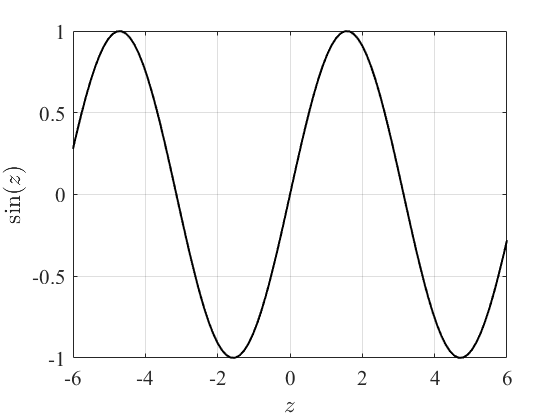
\includegraphics[width=0.35\textwidth]{Pictures/sin.png}
    \end{center}
    \caption[Graph of $\Phi$.]{Graph of $\Phi$ (unconstrained function).}
        \label{fig:sin example 1}
\end{figure}
\begin{figure}[ht!]
    \begin{center}
        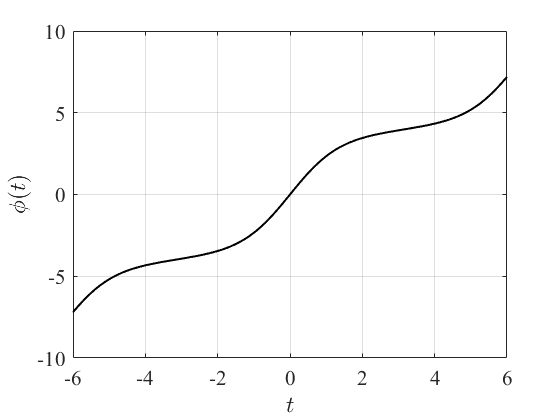
\includegraphics[width=0.35\textwidth]{Pictures/increased_sin.png}
    \end{center}
    \caption[Graph of $\phi = \mathcal{R}_{\mathrm{inc}}\{\Phi\}$.]{Graph of $\phi = \mathcal{R}_{\mathrm{inc}}\{\Phi\}$ (after first rectification).}
        \label{fig:sin example 2}
\end{figure}
\begin{figure}[ht!]
    \begin{center}
    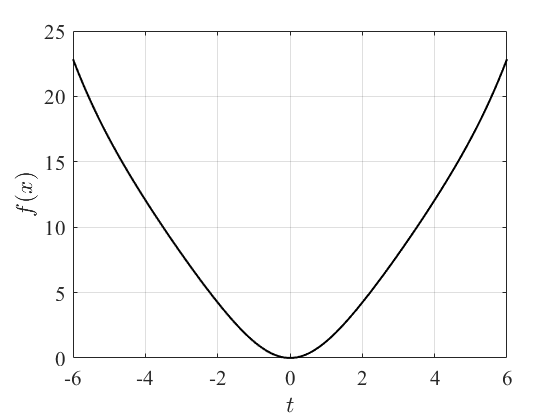
\includegraphics[width=0.35\textwidth]{Pictures/rectified_sin.png}
    \end{center}
    \caption[Graph of $f = \mathcal{R}_{\mathrm{cvx}}\{\phi\} = \mathcal{R}\{\Phi\}$.]{Graph of $f = \mathcal{R}_{\mathrm{cvx}}\{\phi\} = \mathcal{R}\{\Phi\}$ (fully rectified function).}
    \label{fig:sin example 3}
\end{figure}
Notice that in this example, the derivative of the rectified function $f$ cannot be required to vanish at an arbitrary point (as in Eq.~\eqref{eq:constraint-stationarity} for example), since the primary function $\Phi$ is fixed (as opposed to the case where it can be trained). 
\end{remark}


\section{Applications}\label{sec:applications}
We consider a standard setting where data are provided in the form stress-strain responses. For an incompressible material for instance, the Cauchy stress associated with the rectified NN is evaluated as
\begin{equation}
    {\bf\Sigma}^*(\bfF) = 2 {\bfF} \left(\sum_{i = 1}^{3} \frac{\partial w_i^*(I_i)}{ \partial I_i} \frac{\partial I_i}{ \partial \bfC} \right) \bfF^T - p\bfI\,,
\end{equation}
where the left-hand side depends on the parameters of the NN, $w_i^*$ is defined by Eq.~\eqref{eq:def-wistar}, $p$ is a Lagrange multiplier arising from the incompressibility condition (in practice, $p$ is evaluated by imposing a stress-free condition). 

Training with respect to data can be achieved using the cost function
\begin{equation}\label{eq:def-Ld}
     \mathcal{L}_d = \frac{\sum_{i = 1}^{N} \left( \Sigma^*(\bfF(\lambda_i)) - \Sigma^{\textnormal{data}}(\bfF(\lambda_i)) \right)^2}{\sum_{i = 1}^{N} \Sigma^{\textnormal{data}}(\bfF(\lambda_i))^2 }\,,
\end{equation}
along a loading path $\lambda \mapsto \bfF(\lambda)$, discretized with $N$ points. Here, $\Sigma^*$ denotes the relevant stress component (\textit{e.g.}, along testing direction), and $\{(\lambda_i, \Sigma^{\textnormal{data}}(\bfF(\lambda_i)))\}_{i = 1}^{N}$ constitutes the dataset. Note that the above loss function can be readily extended to cases where several loading conditions are considered (see Section \ref{subsec:exp-app}).

In the applications presented below, no attempt was made to fully optimize network architectures and training strategies. The numbers of layers and neurons per layer were determined through a standard parametric analysis on the validation loss defined by Eq.~\eqref{eq:def-Ld}. No activation function was used for the toy problem presented in Section \ref{subsec:toy}, while the sigmoid activation function was selected for all hidden layers in all other examples (in Sections \ref{subsec:MR}, \ref{subsec:anisotropic-app}, and \ref{subsec:exp-app}). 

The Adaptive Moment Estimation (ADAM) algorithm was used for training, with an implementation in JAX \cite{jax2018github}. 

\subsection{Toy Problem}\label{subsec:toy}
We first consider a toy example where the target convex function is given as
\begin{align}
        f^\textnormal{target}(x) = k_1 \exp\left( \frac{(x - k_2)^2}{2k_3^2} \right)\,, \quad \forall x \in \mathbb{R}\,,
\end{align}
where $k_1= 10$, $k_2= 5$, and $k_3= 20$. We seek to construct an approximation over the interval $I = [0, 10]$, centered without loss of generality around the abscissa $x = k_2$ at which $f^\textnormal{target}$ reaches its minimum, with $f(k_2) = k_1$. A set of $100$ equidistant data points is used for fitting, and 20 \% data points are used as the validation set. Adopting the generic notation $\psi$ for the neural network, the rectified model reads as
\begin{equation}
    f(x) = k_1 - \int_{0}^{k_2} \phi(t) \,dt + \int_{0}^x \phi(t) \,dt\,, \quad \forall x \in [0, 10]\,,
\end{equation}
where
\begin{equation}
    \phi(t) = \psi(0) + \int_{0}^t g\left(\frac{d\psi(z)}{dz}\right) \,dz\,.
\end{equation}
Three different choices for $g$ were considered, namely the square function $g(x) = x^2$, the exponential function $g(x) = \exp(x)$, and the modified soft-plus function $g(x) = \log(2^x+1)/\log(2)$. 

In this example, a simple neural network architecture with one hidden layer and two neurons is used (without activation functions). The learning rate for the ADAM optimizer is set to 0.01. Mean square validation errors for the rectified functions are reported in Tab.~\ref{tab:toy-problem-validation-errors} for the three choices of $g$. 
\begin{table}[ht!]
\caption[Results for the validation step (toy problem).]{Results for the validation step: $L^2$-norm errors for the rectified neural network model (toy problem).}
\label{tab:toy-problem-validation-errors}
\begin{center}
    \begin{tabular}{|c|c|} 
        \hline
        Function $g$ & Error $\epsilon$ \\ 
        \hline
        Square & $1.5850 \times 10^{-7}$ \\ 
        \hline
        Exponential & $2.0018 \times 10^{-5}$ \\ 
        \hline
        Soft-plus & $1.6069 \times 10^{-7}$ \\ 
        \hline
        \end{tabular}
\end{center}
\end{table}
The square and modified soft-plus functions provide fairly similar validation errors, smaller than the one obtained with the exponential function. In addition, the model rectified with the square function converged in 3,000 epochs, while the rectified model with the modified soft-plus function converged in about 8,000 epochs. The model with the exponential function converged in more than 10,000 epochs, which is slower than with the other two positive functions. In order to qualitatively assess the accuracy, the predictions obtained with the rectified neural network for the validation dataset are shown in Fig.~\ref{fig:toy-problem-qualitative-results} (see Tab.~\ref{tab:toy-problem-validation-errors} for validation metrics).
\begin{figure}[ht!]
    \begin{center}
        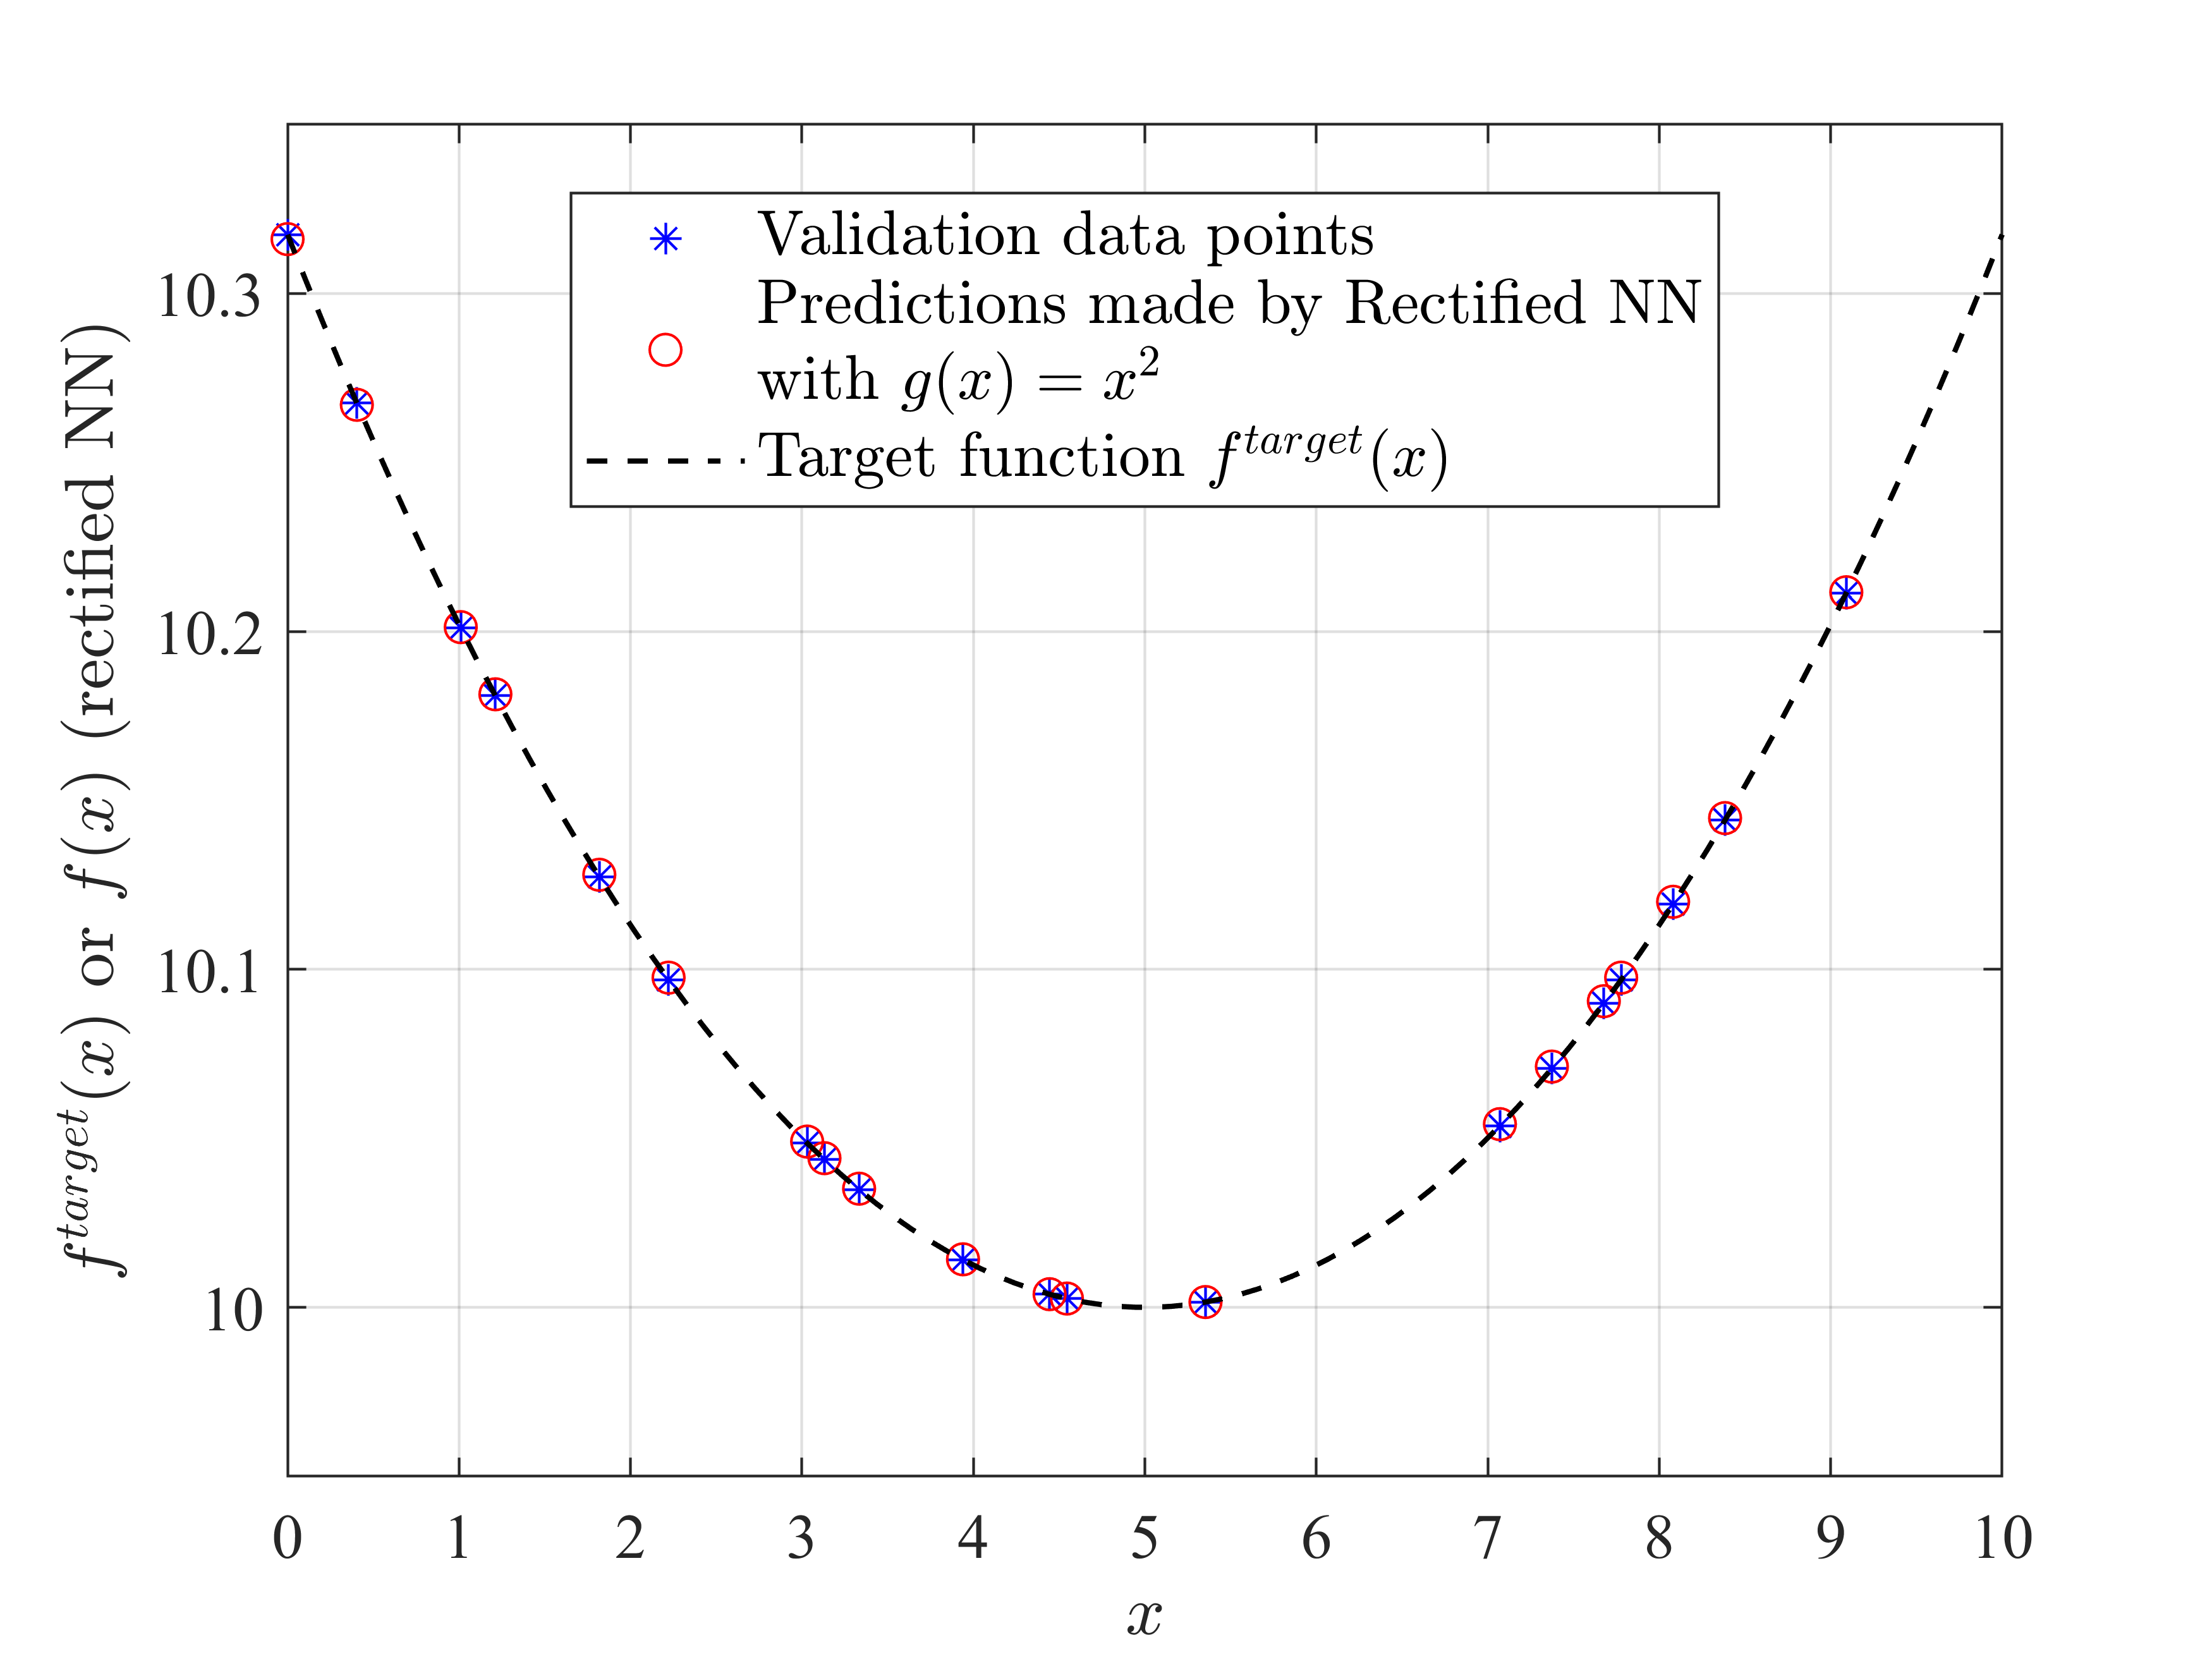
\includegraphics[width = 0.5\textwidth]{Pictures/toy.png}
    \end{center}
    \caption[Target function, reference values, and rectified neural network predictions.]{Target function (black dashed line), reference values (blue star), and rectified neural network predictions (red circles) for the validation dataset (random selection).}
    \label{fig:toy-problem-qualitative-results}
\end{figure}
Recall that no restrictions are imposed on weights and activation functions in the proposed formulation.

\subsection{Mooney-Rivlin Model}\label{subsec:MR}
Here we address the case of a Mooney–Rivlin material, defined by the stored energy function
\begin{equation}
    w{^\textnormal{MR}}(I_1,I_2) = C_1(I_1 - 3) + C_2(I_2 - 3)\,, \label{eq:MR}
\end{equation}
where $C_1$ and $C_2$ are strictly positive material parameters (see \cite{ciarlet1988mathematical}, p.~189). The rectified model is written as
\begin{equation}
    w^*(I_1, I_2) = w_1^*(I_1) + w_2^*(I_2)\,,
\end{equation}
with 
\begin{align}
    w_1^*(I_1) = \mathcal{R}\{\psi_1(\{\bfW_j^{(1)}, \bfb_j^{(1)}\}_{j = 1}^{n_1})\}(I_1)
\end{align}
and
\begin{align}
w_2^*(I_2) = \mathcal{R}\{\psi_2(\{\bfW_j^{(2)}, \bfb_j^{(2)}\}_{j = 1}^{n_2})\}(I_2)\,.
\end{align}
The Cauchy stress is given by (see \cite{HolzapfelBook}, p. 224)
\begin{equation}
    \boldsymbol{\Sigma} = 2C_1\bfB - 2C_2\bfB^{-1} - p \bfI\,.
\end{equation}
We consider uniaxial tension along the first direction for training purposes, in which case the uniaxial Cauchy stress writes 
\begin{equation}
    \Sigma(\lambda) = 2\left(C_1 + \frac{ C_2}{\lambda}\right)\left(\lambda^2 - \frac{1}{\lambda}\right)\,, \label{eq:MR_Cauchy}
\end{equation}
where $\lambda$ is the driving principal stretch. The uniaxial Cauchy stress associated with the rectified model can be evaluated as
\begin{equation}
    \Sigma^*(\lambda) = 2 \left( \frac{\partial w_1^*(I_1)}{\partial I_1} + \frac{\partial w_2^*(I_2)}{\partial I_2} \frac{1}{\lambda} \right) \left( \lambda^2 - \frac{1}{\lambda} \right)\,, 
\end{equation}
with
\begin{equation}
    \frac{\partial w_i^*(I_i)}{\partial I_i} =  \left( \psi_i(0) + \int_0^{I_i} g\left(\frac{d\psi_i}{dz}\right)\, dz \right)\,.
\end{equation}
Derivatives are computed using automatic differentiation. In this example, we consider an approximation for $\lambda \in [1.0, 1.4]$ ($I_1 \geq 3$ and $I_2 \geq 3$). The material parameters are arbitrarily chosen as $C_1 = 10$ and $C_2 = 5$. Normalization condition is imposed by taking $w_1^*(3) = w_2^*(3) = 0$ with the constant terms (see Eq.~\eqref{eq:Rec-Con}, with $a = 3$) set to 0. Note that the stress free condition is automatically satisfied owing to the definition of $p$.

Two hundreds datapoints are generated using Eq.~\eqref{eq:MR_Cauchy}, with 20 \% of samples allocated for validation.  Parametric studies on validation error were conducted to identify the NN architecture, using a learning rate set to $0.01$, 5,000 epochs, and the square function (in the first rectifier); see Fig.~\ref{fig:Mr_Err_Study}.
\begin{figure}[ht!]
    \begin{center}
        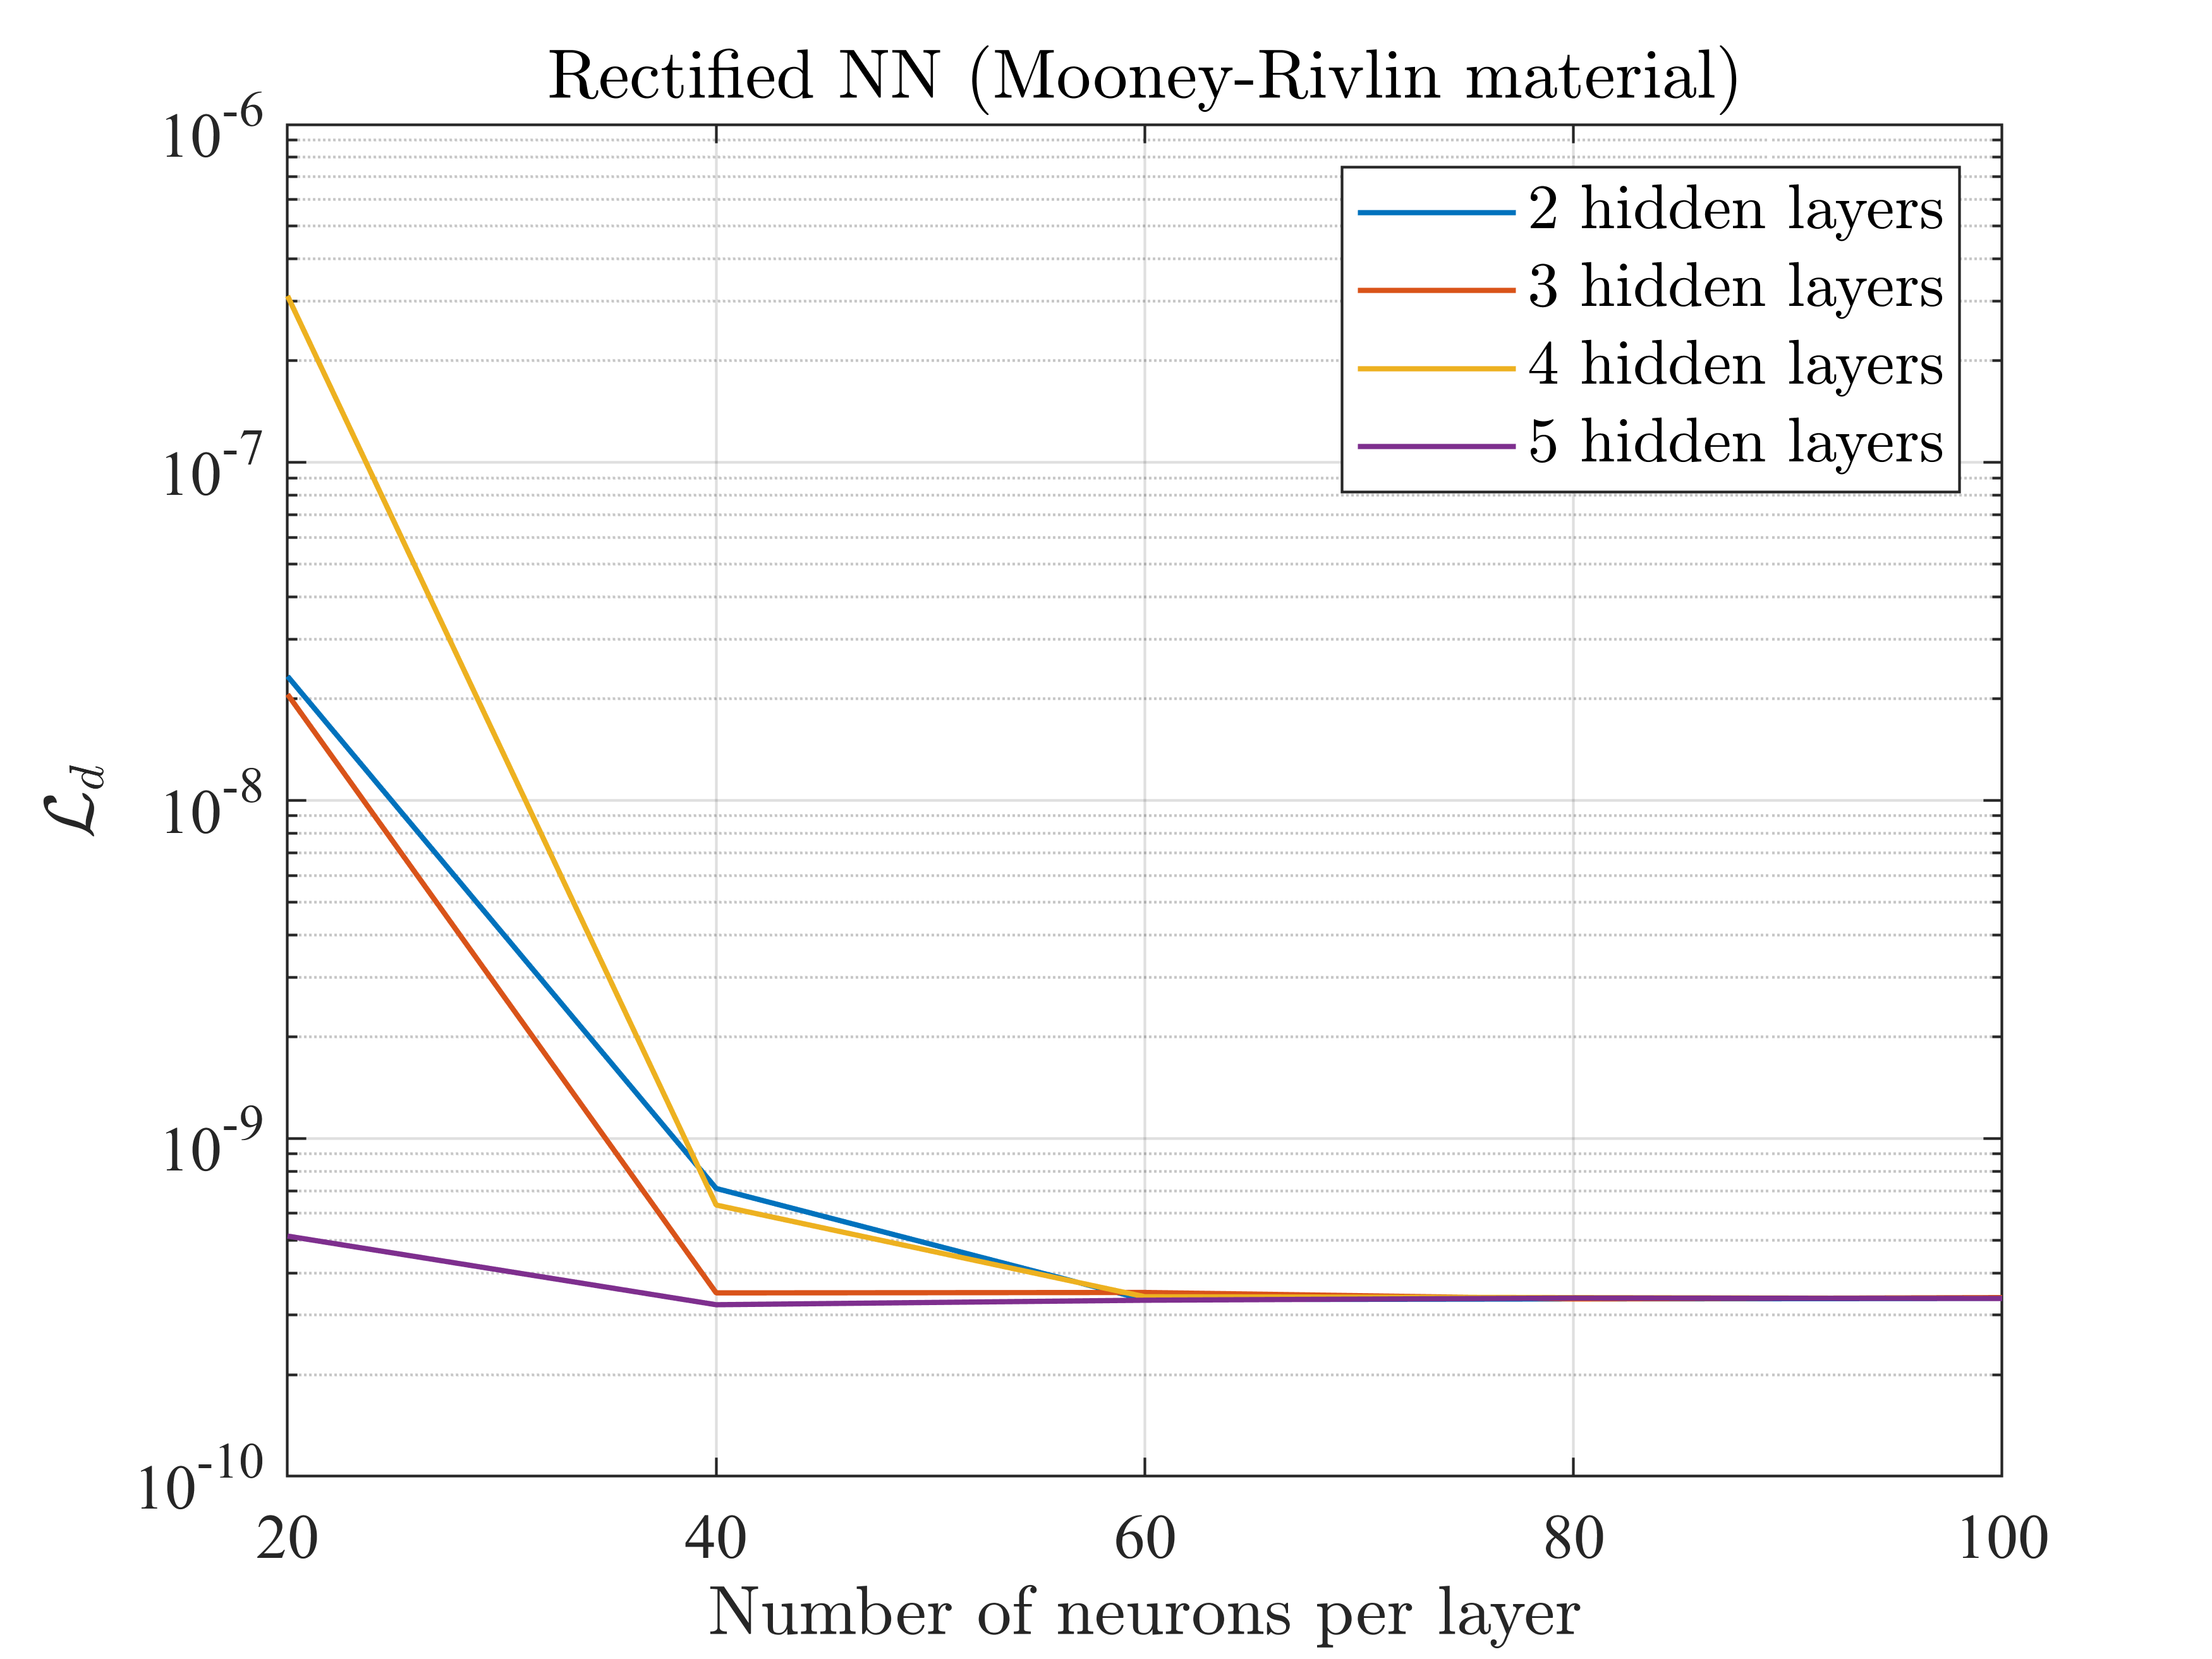
\includegraphics[width = 0.5\textwidth]{Pictures/Mr_Err.png}
    \end{center}
    \caption[Loss $\mathcal{L}_d$ for different neural network architectures.]{Loss $\mathcal{L}_d$ for different neural network architectures on the validation dataset (Mooney-Rivlin material).}
    \label{fig:Mr_Err_Study} 
\end{figure}
Results predicted by the calibrated rectified neural network model (with 5 layers and 40 neurons per layer) on the validation dataset is shown in Fig.~\ref{fig:MR best result 1}.
\begin{figure}[ht!]
    \begin{center}
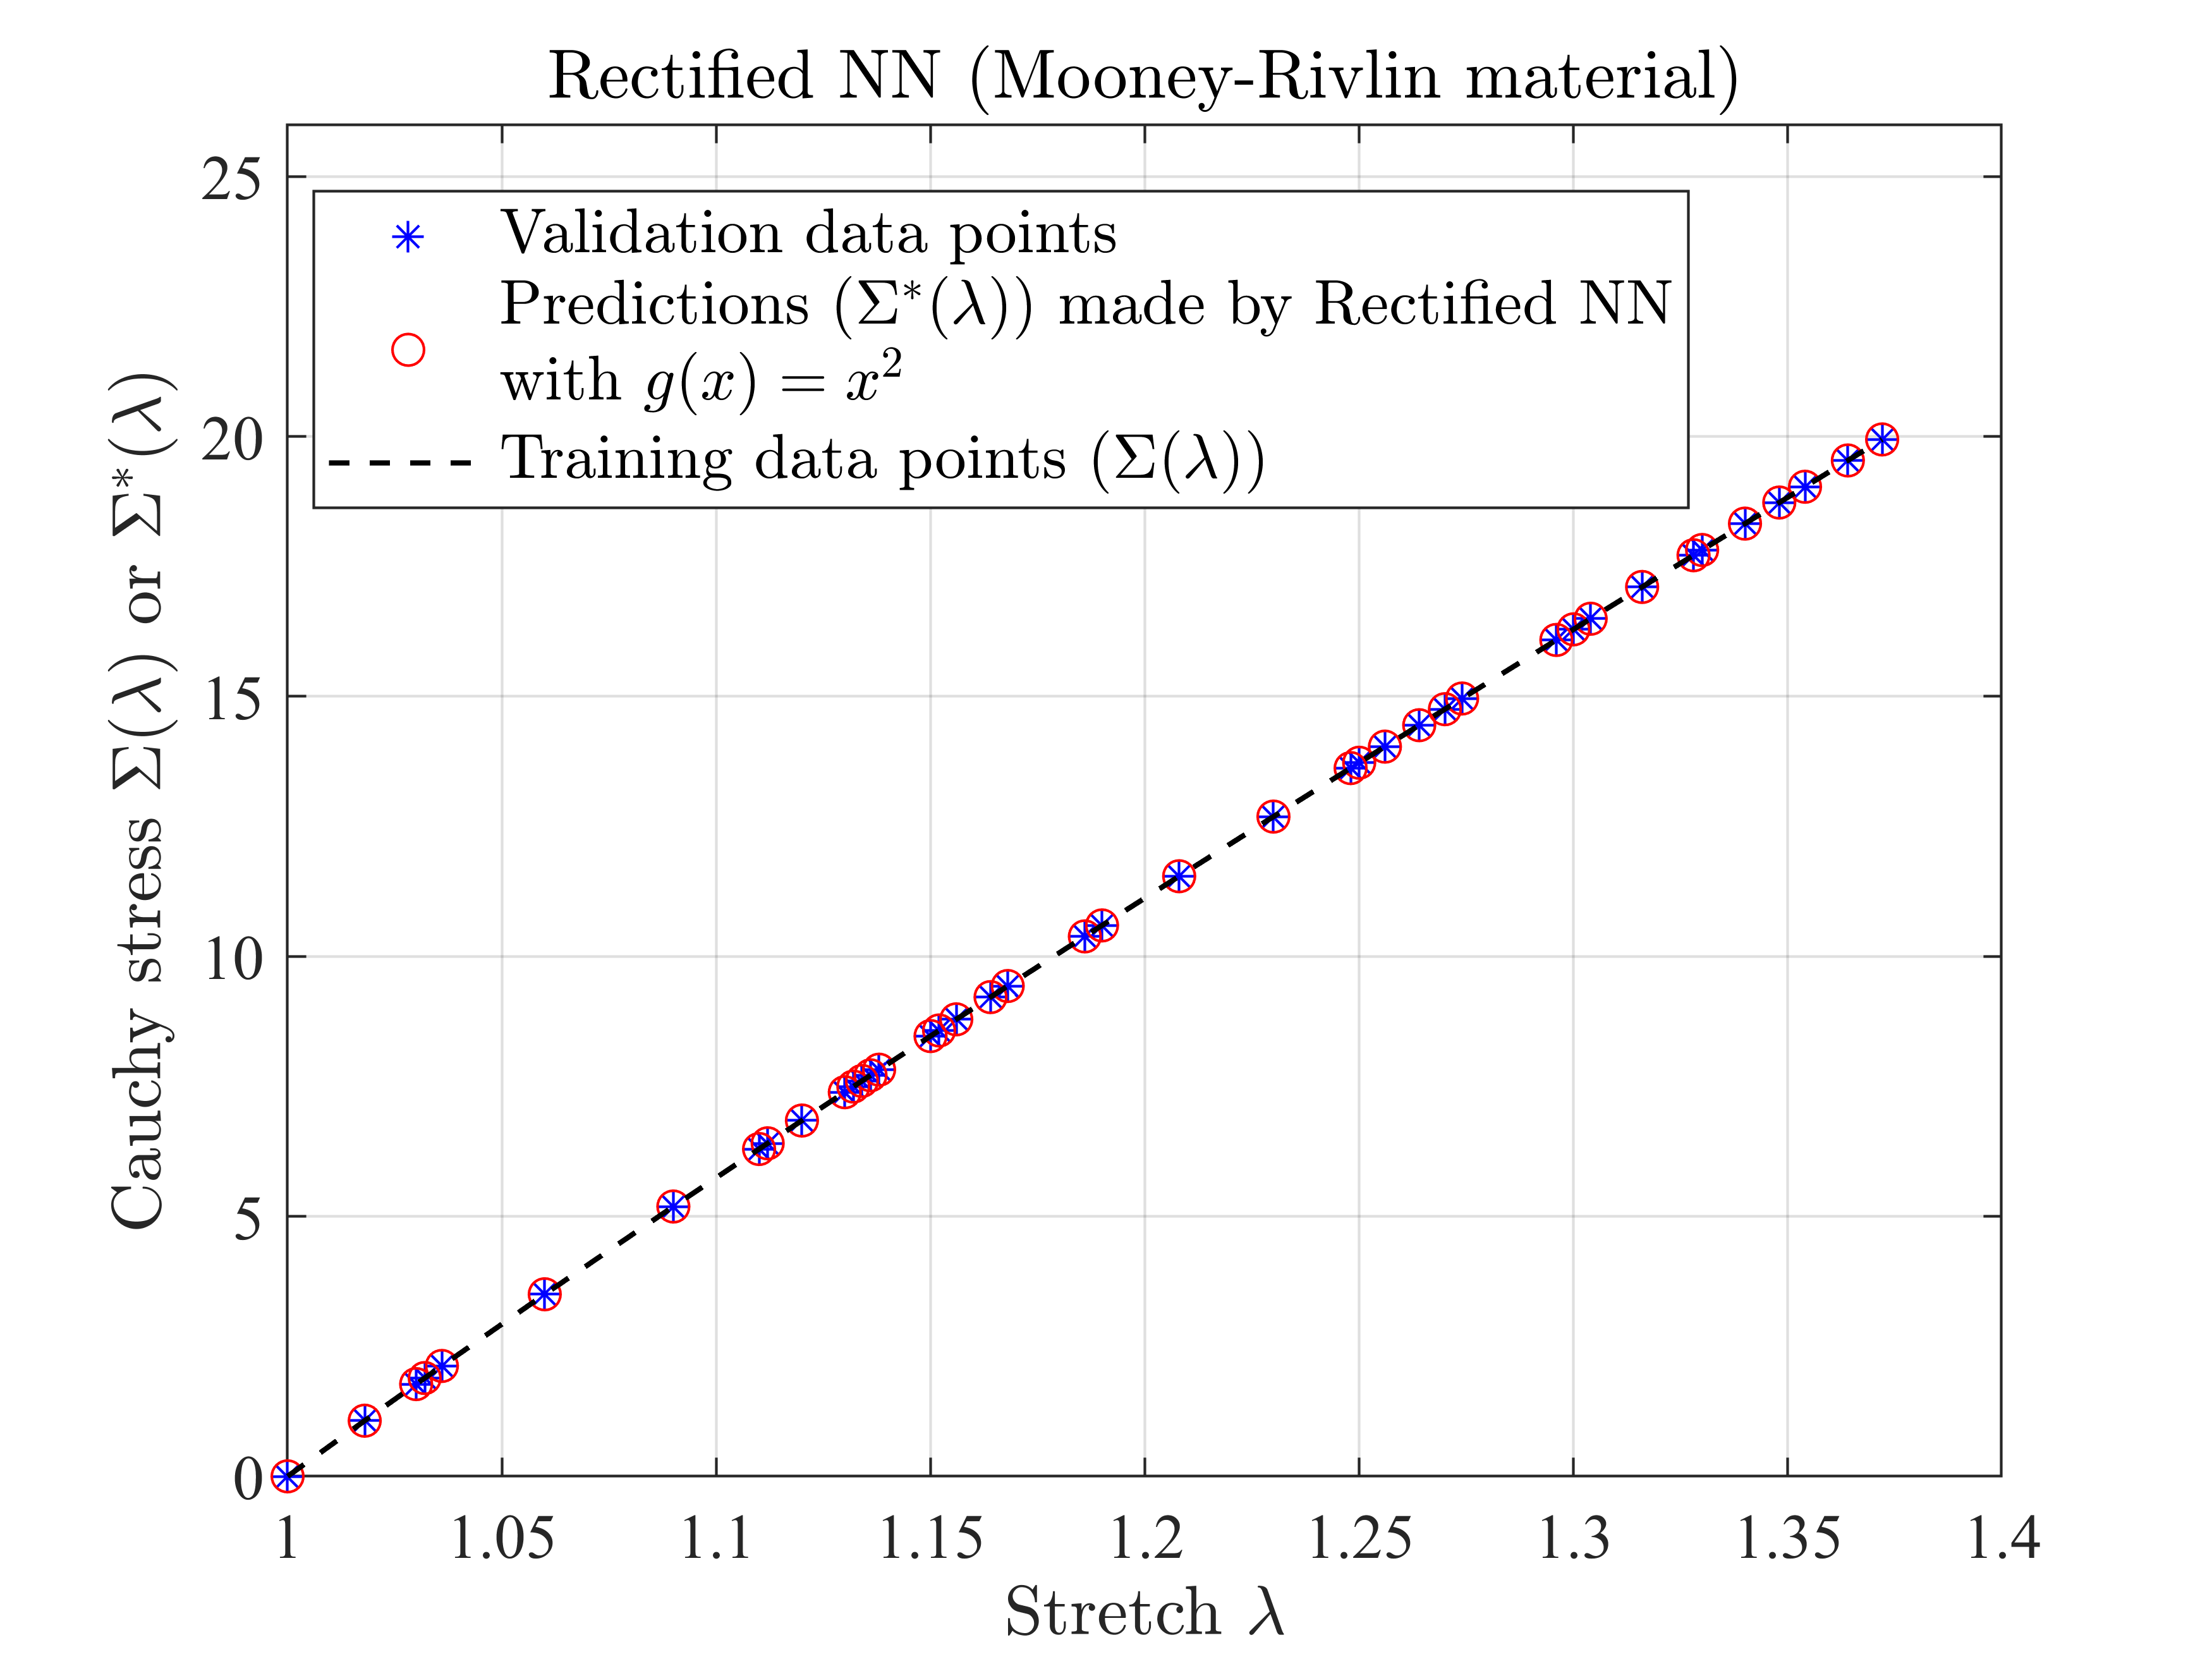
\includegraphics[width=0.5\textwidth]{Pictures/sigma_MR.png}
    \end{center}
    \caption[Reference stress response and values, rectified NN predictions.]{Reference stress response $\lambda \mapsto \Sigma(\lambda)$ (black dashed line), reference values (blue star), and rectified neural network predictions (red circle) for the validation dataset (random selection). Here, 5 hidden layers and 40 neurons per layer are used.}
    \label{fig:MR best result 1}
\end{figure}

\begin{remark} As indicated before, Input-Convex Neural Networks (ICNNs) can be obtained by forcing all weights, except those connected to the input, to be non-negative, and by using only convex non-decreasing activation functions \cite{amos2017input, as2022mechanics,Asad-IJNME,KLEIN2022104703}. In order to evaluate the performance of such constrained neural networks in terms of training results, we consider a model of the form 
\begin{align}
    \psi_{\mathrm{ICNN}}(I_1, I_2) &= \psi_{\mathrm{ICNN}}^{(1)}(I_1) + \psi_{\mathrm{ICNN}}^{(2)}(I_2)\,,
\end{align}
where each ICNN involves unconstrained weights that are mapped to positive weights in the loss function, using the modified soft-plus activation function proposed in \cite{as2022mechanics,Asad-IJNME}. The validation loss history for each approach is shown in Fig.\ref{fig:ERR_history} for the Mooney-Rivlin dataset.
\begin{figure}[ht!]
    \begin{center}
        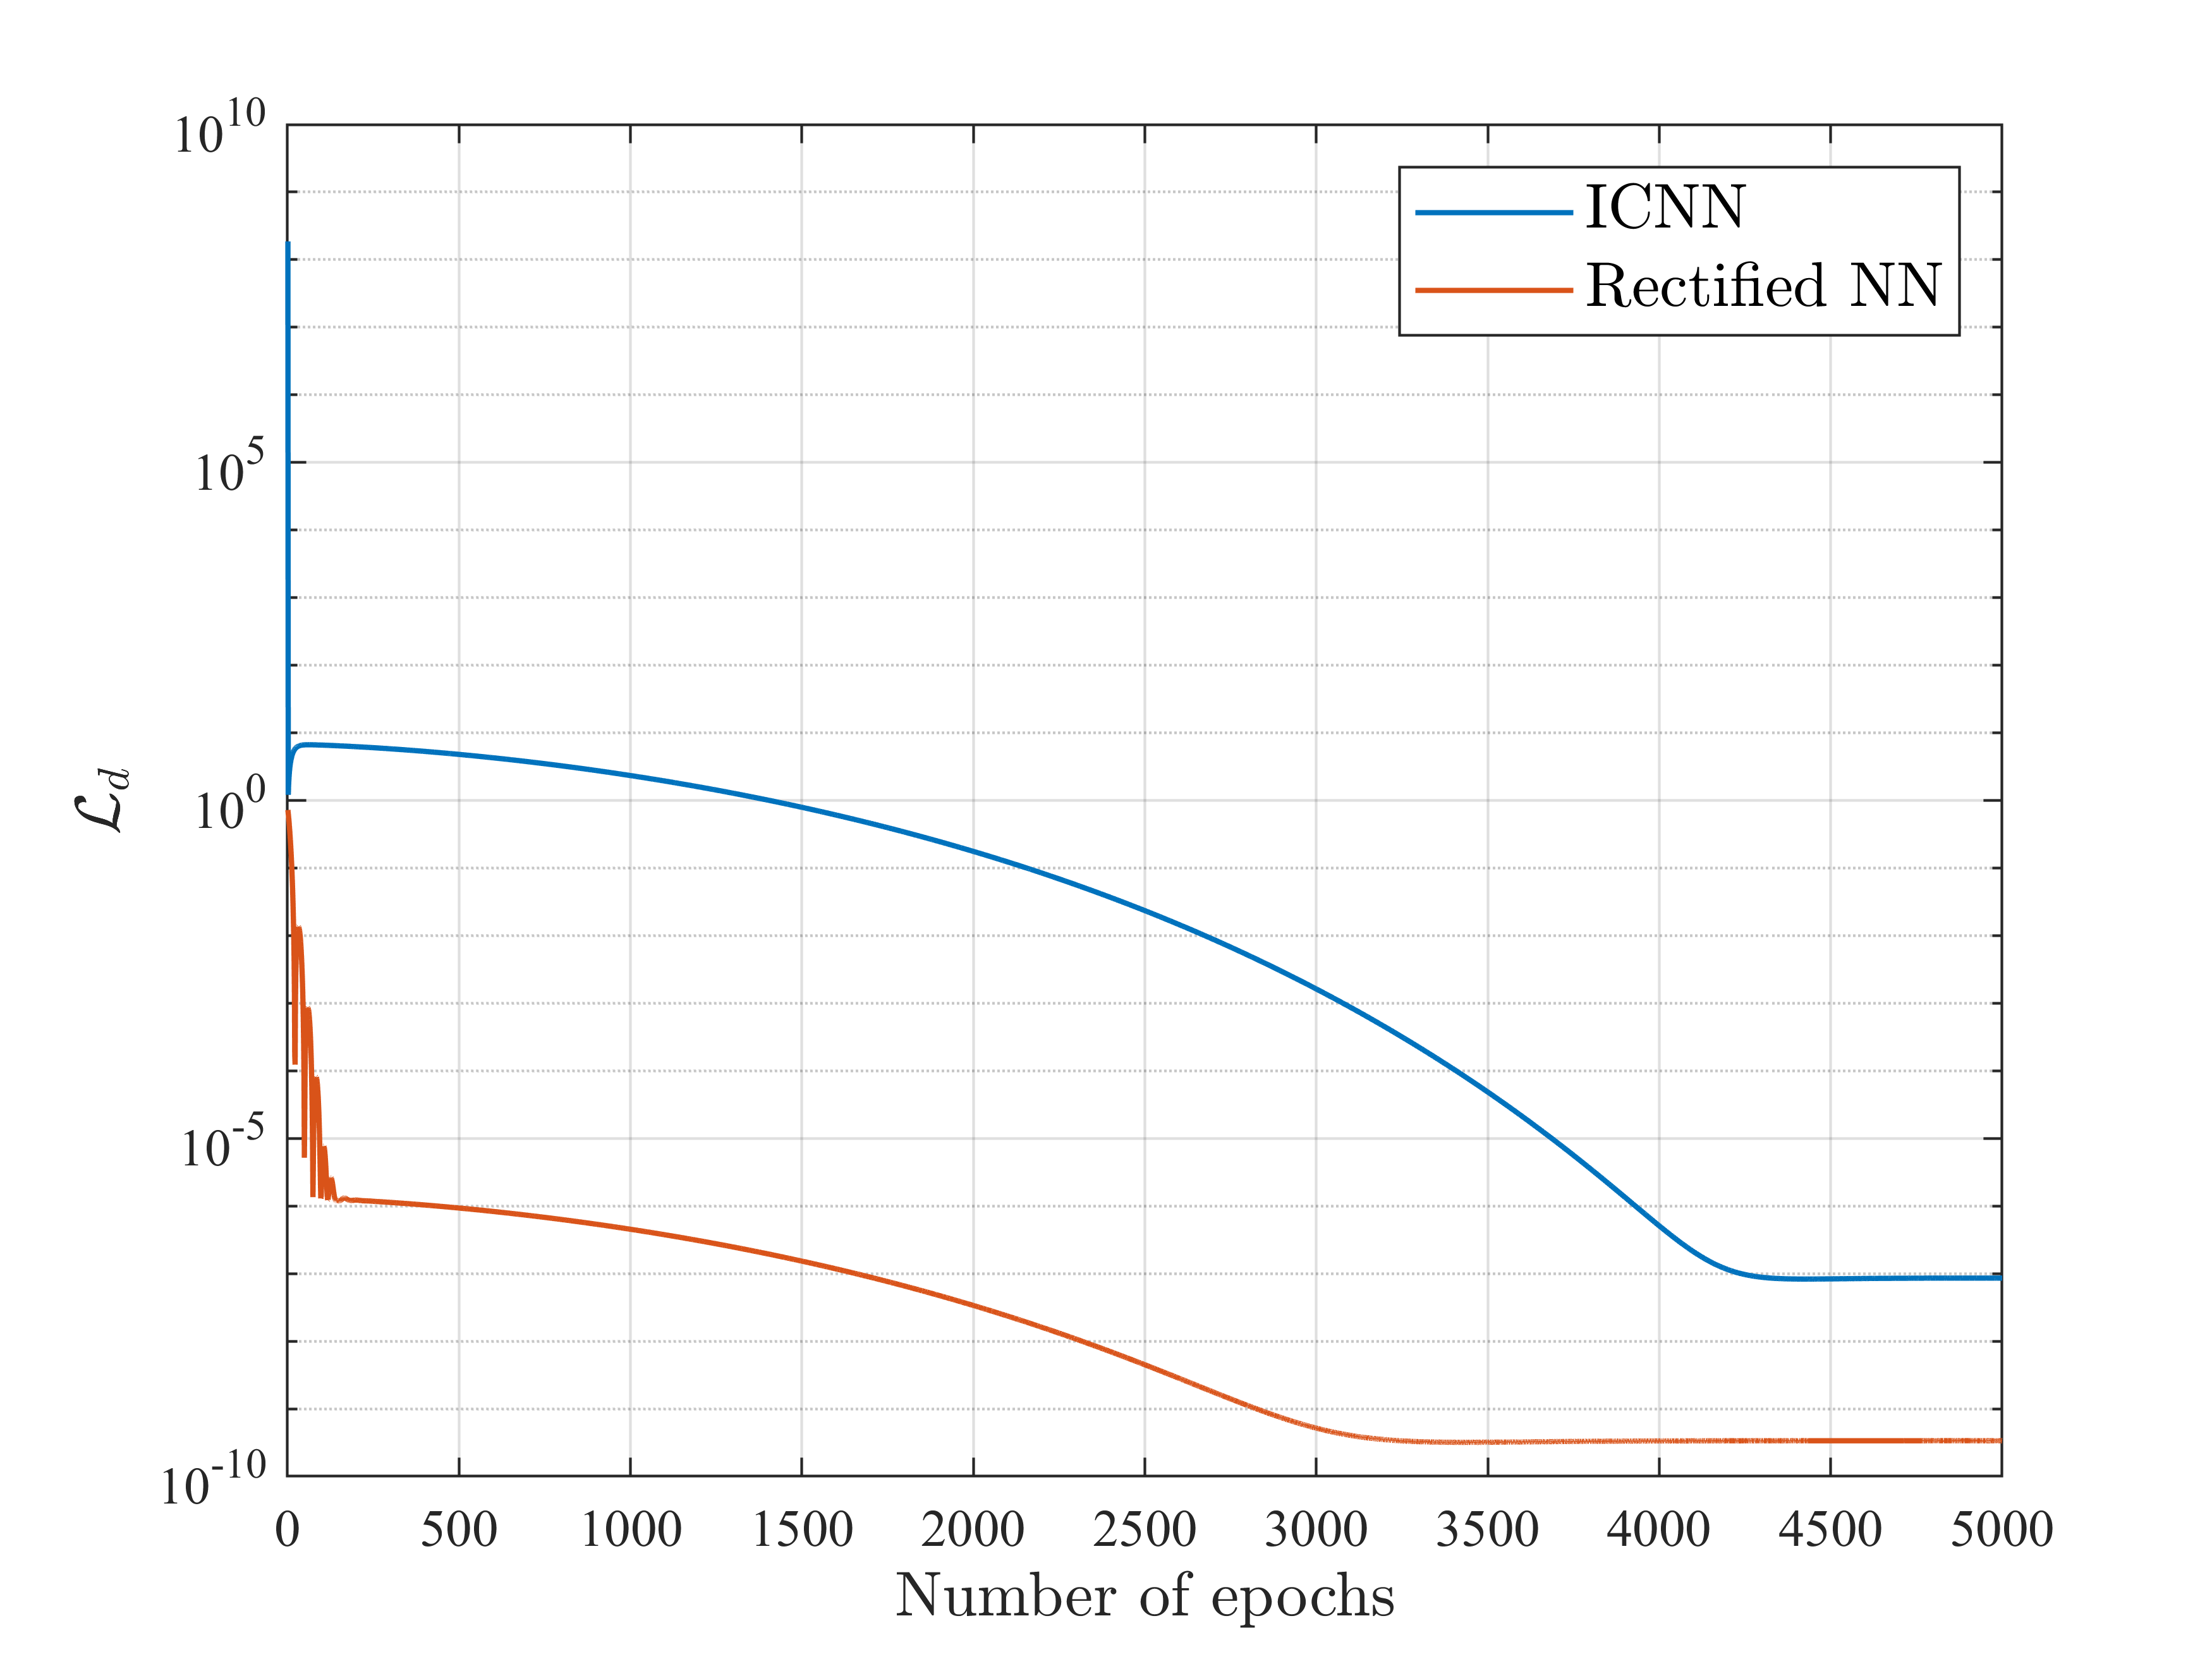
\includegraphics[width = 0.5\textwidth]{Pictures/loss_hist.png}
    \end{center}
    \caption[Loss history for ICNN and the proposed rectified NN.]{Loss history for ICNN and the proposed rectified NN.}
    \label{fig:ERR_history} 
\end{figure}
Reported results were obtained with 2 hidden layers and 20 neurons per layer for both strategies, based on a parametric convergence study on the validation metric. It is seen that the rectified NN converges much faster than the ICNN and leads to a lower training error. While similar results were obtained for a wide range of architectures, it should be pointed out that the computational cost per iteration is greater in the case of rectified NNs, which require numerical integration to be performed. In addition, opposite trends with respect to learning rates were observed: ICNNs tend to perform slightly better at large learning rates (\textit{e.g.}, 1.5) but require a very large number of iterations (greater than 40,000) at standard learning rates (\textit{e.g.}, 0.001). These observations are most likely imputable to the transformation of negative weights, which generates large regions with ``flat'' gradients in the optimization process. In contrast, rectified NNs were found to perform steadily in terms of training cost, regardless of the learning rate, and typically performs (much) better at smaller rates. An extensive comparison of the tradeoffs between these approaches is left for future work.
\end{remark}

\subsection{Anisotropic Model for Digital Dataset} \label{subsec:anisotropic-app}
We next consider an anisotropic strain energy density function, relevant to the modeling of soft biological tissues such as arterial vessels \cite{balzani2006polyconvex,staber2018stochastic}. It should be noticed such materials are often modeled as nearly-incompressible in a computational setting, in which case the strain energy density function is typically expressed in terms of isochoric invariants. The reference function is defined as
\begin{equation}
    w(I_1, I_2, J_4^{(1)}, J_4^{(2)}) = w{^\textnormal{MR}}(I_1,I_2) + w{^\textnormal{A}}(J_4^{(1)}, J_4^{(2)})\,,
\end{equation}
where $w{^\textnormal{MR}}$ is given by Eq.~\eqref{eq:MR} and the anisotropic term is defined as
\begin{equation}
    w{^\textnormal{A}}(J_4^{(1)}, J_4^{(2)}) = \sum_{k=1}^2 w^{\text{ti}} (J_4^{(k)})\,,
\end{equation}
with
\begin{align}
    w^{\text{ti}} (J_4^{(k)}) = \frac{\mu_4}{\beta_4} \left\{ \exp \left(\beta_4 w^B(I_1, J_4^{(k)}) \right) - 1\right\} \label{eq: psi tissue}
\end{align}
where $w^B(I_1, J_4^{(k)}) = (1-\rho)(I_1 - 3)^2 + \rho \langle J_4^{(k)} - 1 \rangle_m^2$, and $J_4^{(k)}= \tr(\bfC \bfM^{(k)})$. The structural tensors $\bfM^{(k)} = \bfa^{(k)} \otimes \bfa^{(k)}$ are defined in terms of the unit vectors 
\begin{subequations}
    \begin{align}
        \bfa^{(1)} &= \cos(\alpha) \bfe^{(1)} + \sin(\alpha)\bfe^{(2)}\,, \\ 
        \bfa^{(2)} &= \cos(\alpha) \bfe^{(1)} - \sin(\alpha)\bfe^{(2)}\,,
    \end{align}
\end{subequations}
where $\bfe^{(1)}$ and $\bfe^{(2)}$ are unit basis vectors and $\alpha$ is the angle defining the directions of anisotropy. In Eq.~\eqref{eq: psi tissue}, $\mu_4$, $\beta_4$, and $\rho$ are material parameters, and $\langle \cdot \rangle_m$ denotes the Macaulay bracket. Note that the angle $\alpha$ is also considered as a trainable parameter.

The rectified neural network is sought as
\begin{equation}\label{eq:rec-model-anisotropic-case}
    w_1^*(I_1) + w_2^*(I_2) + w_3^*(J_4^{(1)}) + w_4^*(J_4^{(2)})\,,
\end{equation}
where
\begin{equation}
    w_i^*(I_i) = \mathcal{R}\{\psi_i(\{\bfW_j^{(i)}, \bfb_j^{(i)}\}_{j = 1}^{n_i})\}(I_i)\,,\quad i=1,2\,,
\end{equation}
\begin{align}
    w_{3}^*(J_4^{(1)}) = \mathcal{R}\{\psi_3(\{\bfW_j^{(3)}, \bfb_j^{(3)}\}_{j = 1}^{n_3})\}(J_4^{(1)})\,,
\end{align}
and
\begin{align}
    w_{4}^*(J_4^{(2)}) = \mathcal{R}\{\psi_4(\{\bfW_j^{(4)}, \bfb_j^{(4)}\}_{j = 1}^{n_4})\}(J_4^{(2)})\,.
\end{align}
Biaxial tension is used for training purposes. The Cauchy stress associated with the reference model is obtained as
\begin{align}
     \Sigma(\lambda) = \Sigma^{\text{MR}}(\lambda) + \Sigma_{(1)}^{\text{ti}} (\lambda) + \Sigma_{(2)}^{\text{ti}} (\lambda)\,,
\end{align}
with
\begin{equation}
    \Sigma^{\text{MR}}(\lambda) = 2C_1(\lambda^2 - \frac{1}{\lambda^4}) - 2C_2(\frac{1}{\lambda^2} - \lambda^4)\,,
\end{equation}
and
\begin{align}
    \Sigma^{\text{ti}}_{(k)}(\lambda) = & \, 4 \lambda^2 \mu_4 \left\{ (1-\rho)(I_1 - 3)\left(1 - \frac{1}{\lambda^6}\right) \right.  \nonumber \\
    & \quad + \left. \rho \langle J_4^{(k)} - 1 \rangle_m \cos^2(\alpha) \right\}  \nonumber\\
    &\quad \times \exp(\beta_4 w^B(I_1, J_4^{(k)}))\,, \quad k = 1,2\,.
\end{align}
with a slight abuse of notation. The Cauchy stress for the rectified model defined by Eq.~\eqref{eq:rec-model-anisotropic-case} is given by
\begin{align}\label{eq:ANI_Cauchy}
    \Sigma^{*} = \Sigma^*_1(\lambda) + \Sigma^*_2(\lambda) +  \Sigma^*_3(\lambda) + \Sigma^*_4(\lambda)\,,
\end{align}
where terms in the right-hand side are defined as $\Sigma^*_1(\lambda) = 2 \frac{\partial w_1^*(I_1)}{\partial I_1} \left( \lambda^2 - \frac{1}{\lambda^4} \right)$, 
\begin{equation}
    \Sigma^*_1(\lambda) = 2 \frac{\partial w_1^*(I_1)}{\partial I_1} \left( \lambda^2 - \frac{1}{\lambda^4} \right)\,, 
\end{equation}
\begin{equation}
    \Sigma^*_2(\lambda) = -2 \frac{\partial w_2^*(I_2)}{\partial I_2} \left(\frac{1}{\lambda^2} - \lambda^4 \right)\,,
\end{equation}
\begin{equation}
    \Sigma_3^*(\lambda) = 2 \lambda^2 \frac{\partial w_3^*(J_4^{(1)})}{\partial J_4^{(1)}} \cos^2(\alpha)\,,
\end{equation}
\begin{equation}\label{eq:aniso-last-stress-component}
    \Sigma_4^*(\lambda) = 2 \lambda^2 \frac{\partial w_4^*(J_4^{(2)})}{\partial J_4^{(2)}} \cos^2(\alpha)\,.
\end{equation}
Since $\cos(\alpha) \neq 0$ in practice, the stress free constraint reduces to $\Sigma^*_3(1) + \Sigma^*_4(1) = 0$.
% \begin{align}\label{eq:stress-free-constraint-anisotropic-model}
%     \Sigma^*_3(1) + \Sigma^*_4(1) = 0\,.
% \end{align}
In the numerical example below, the material parameters correspond to the values identified in \cite{CHEN2022114897} for sample \#10 in the media layer: $C_1 = 0.7071$ [kPa], $C_2 = 0.0531$ [kPa], $\alpha = 0.2740$ [rad], $\mu_4 = 15.5753$ [kPa], $\beta_4 = 2.5561$, and $\rho = 0.0986$. Similarly to the previous case, we generated 200 datapoints, 20\% of which are used as the validation set. The learning rate is set to 0.005 for the first 3,000 epochs and then to 0.001 for 3,000 epochs, and presented results were obtained using the exponential function in the rectifier (i.e., $g(x) = \exp(x)$). The validation errors for different neural network architectures are shown in Fig.~\ref{fig:ani_err}.
\begin{figure}[ht!]
    \begin{center}
    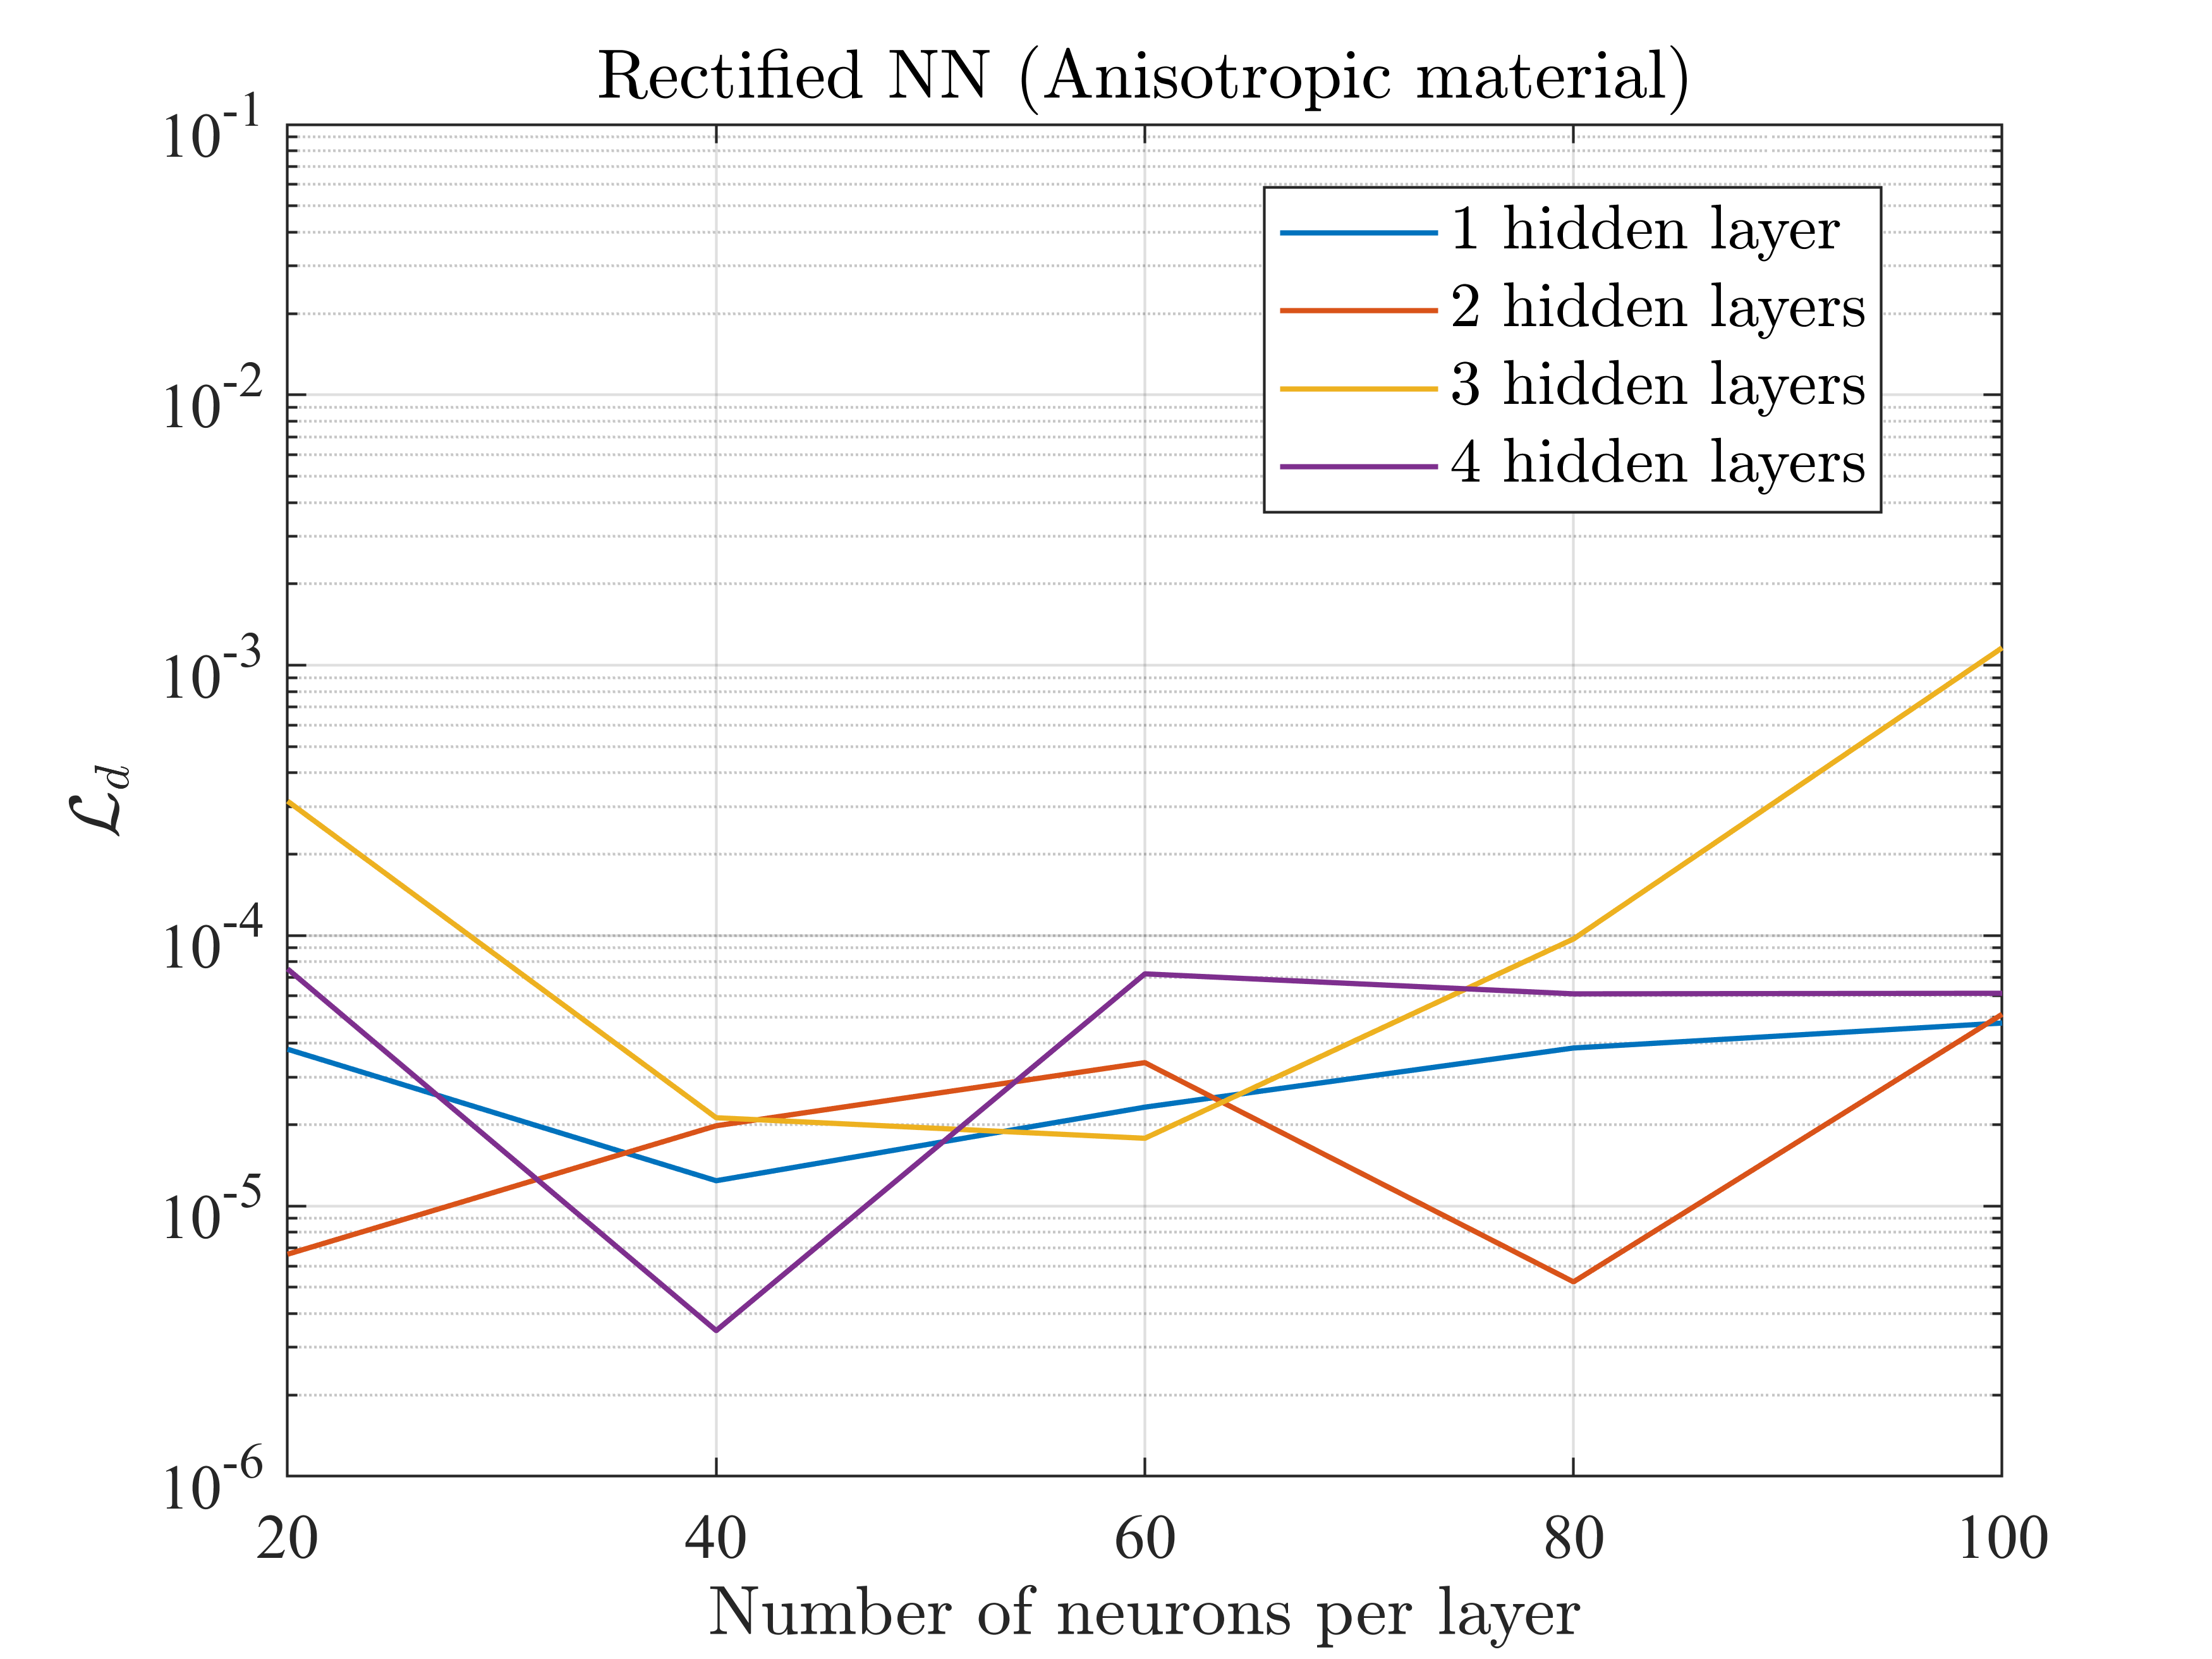
\includegraphics[width=0.5\textwidth]{Pictures/ANI_ERR.png}
    \end{center}
    \caption[Parametric study for RNN architectures.]{Parametric study of the mean squared error for different NN architectures on the validation dataset (Anisotropic material).}
    \label{fig:ani_err}
\end{figure}
Results predicted with the fitted rectified neural network model on the validation dataset are shown in Figs.~\ref{fig:ANI best result 1}.
\begin{figure}[ht!]
    \begin{center}
        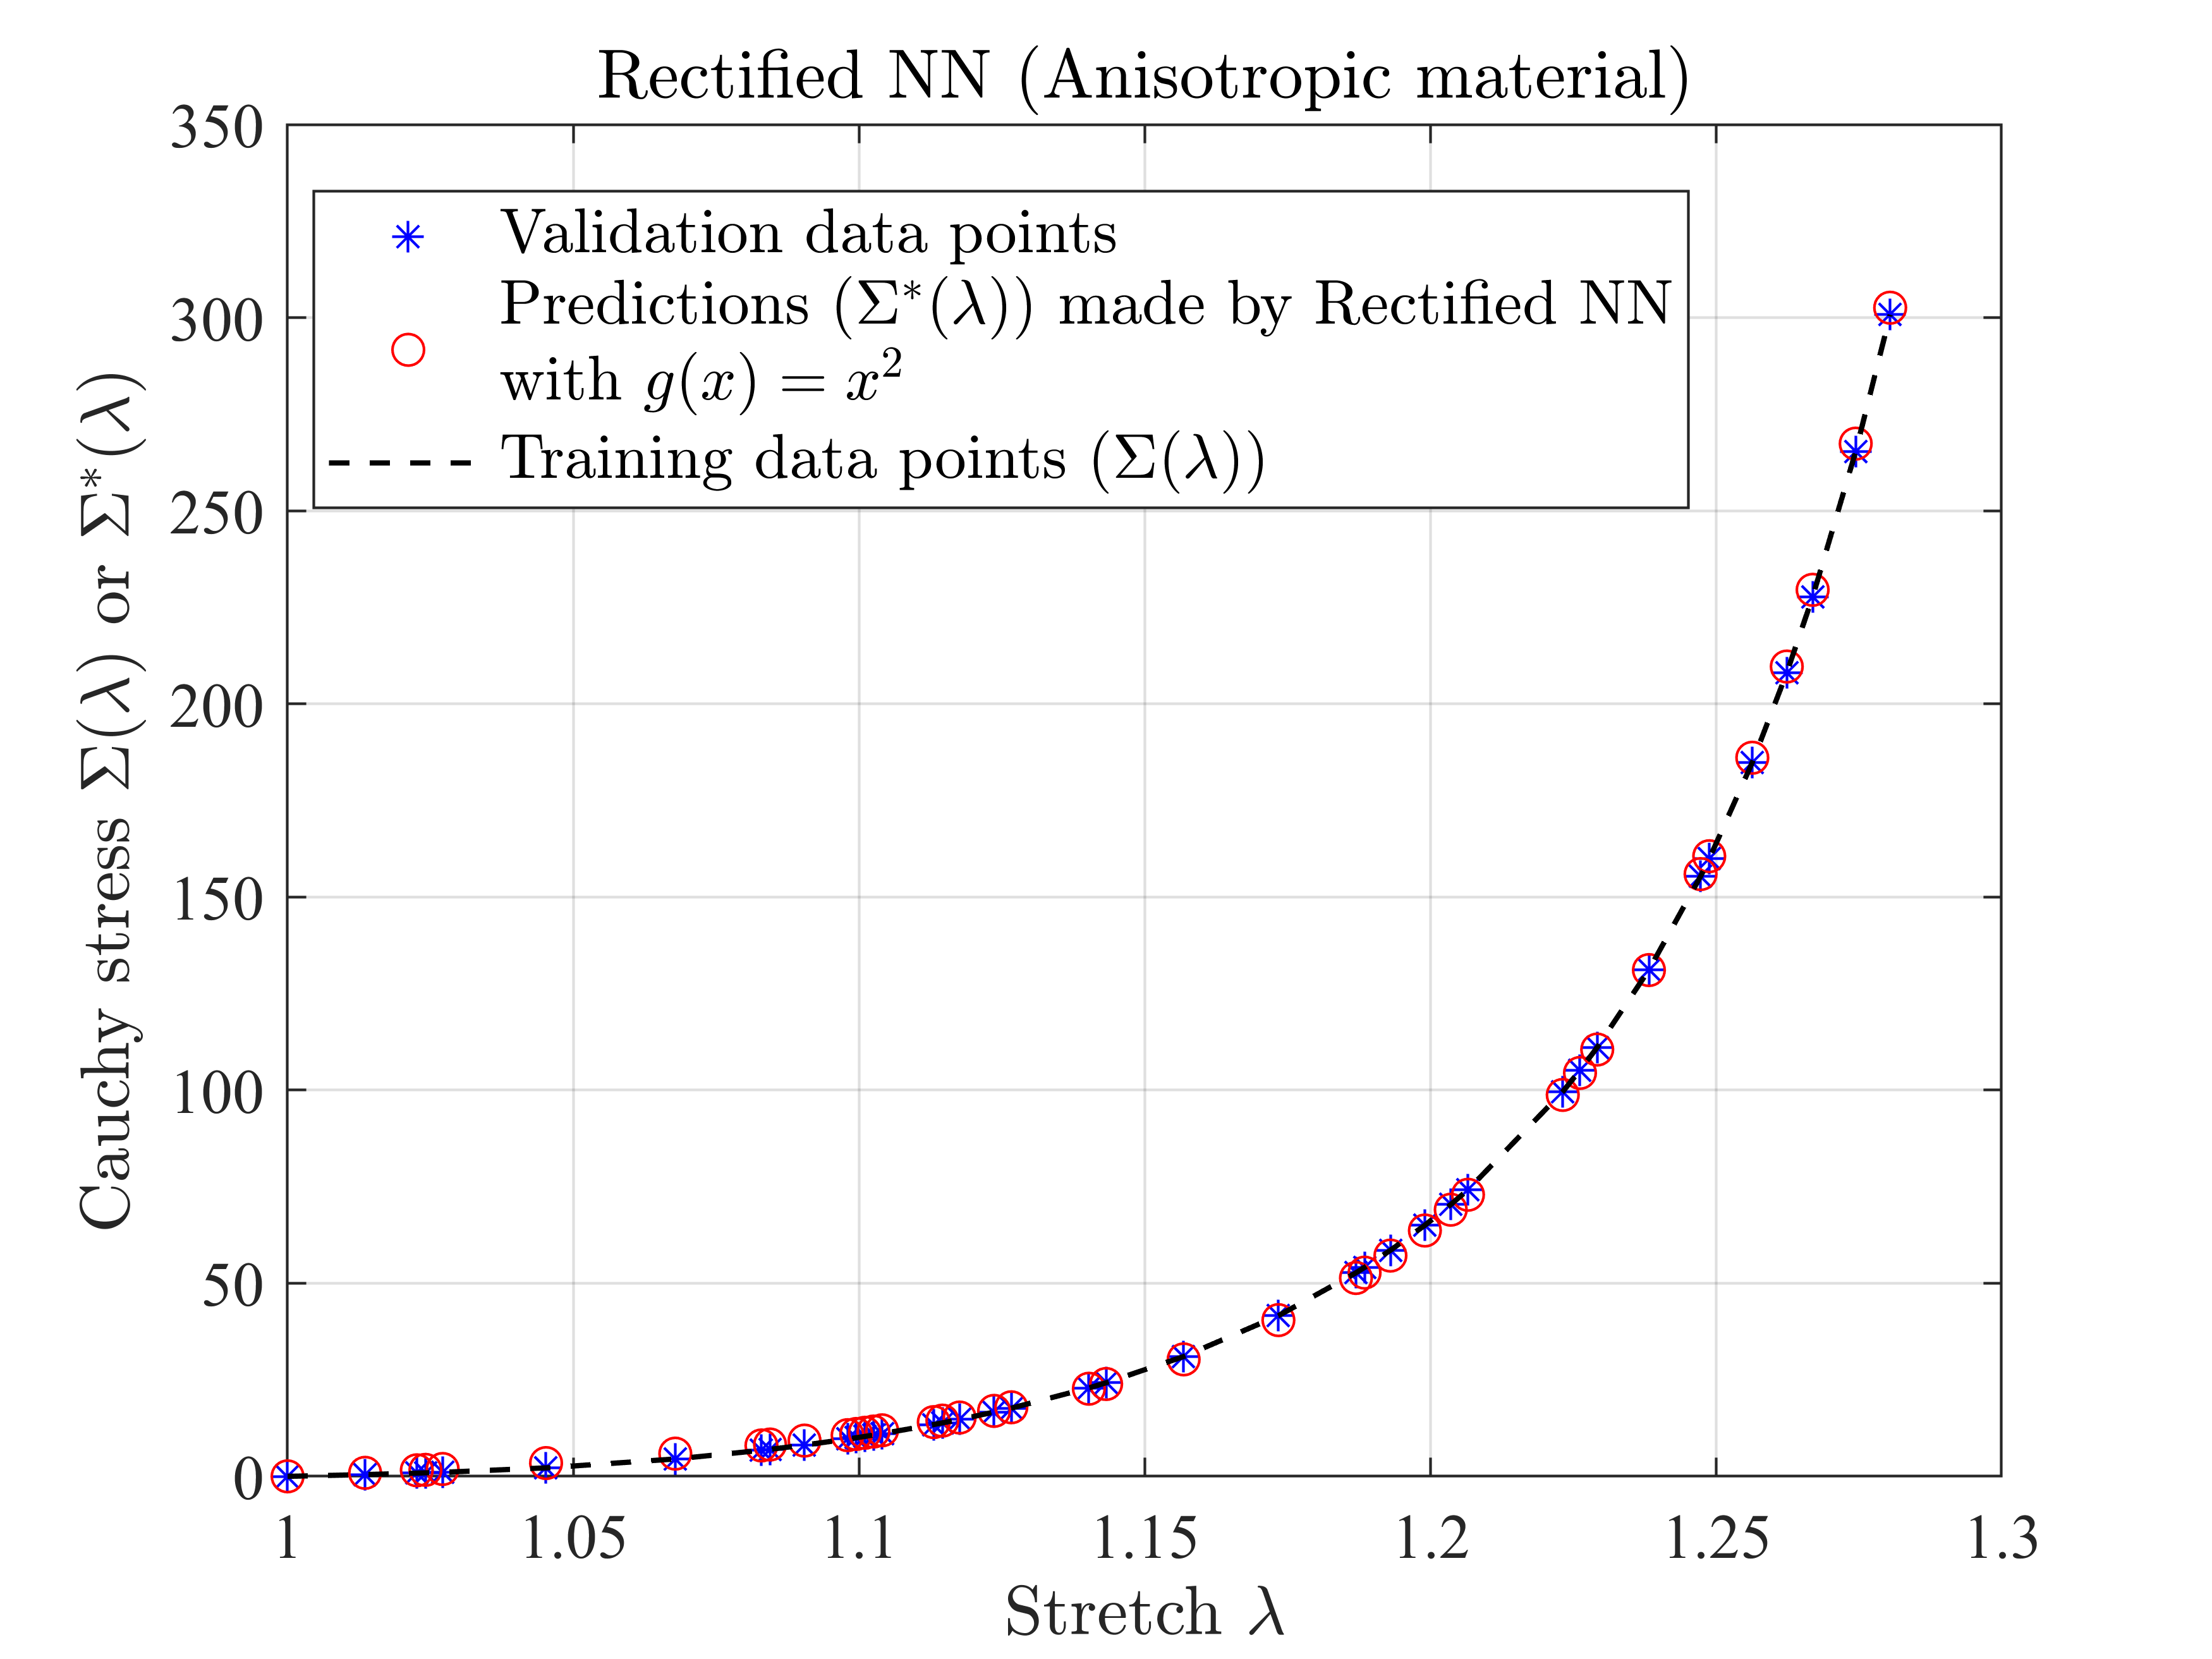
\includegraphics[width=0.5\textwidth]{Pictures/sigma_ANI.png}
    \end{center}
    \caption[Reference stress response and values, rectified NN predictions.]{Reference stress response $\lambda \mapsto \Sigma(\lambda)$ (black dashed line), reference values (blue star), and rectified neural network predictions (red circle) for the validation dataset (random selection). Here, the NN involves 4 hidden layers and 40 neurons per layer.}
    \label{fig:ANI best result 1}
\end{figure}
The validation metric in this example is $3.46 \times 10^{-6}$.

\subsection{Anisotropic Model for Experimental Dataset}\label{subsec:exp-app}
We finally apply the proposed rectification method to the experimental dataset presented in \cite{holzapfel2005determination}, corresponding to uniaxial extension tests on human illiac arterial walls. In those experiments, two different strips were harvested along the circumferential and longitudinal directions on each specimen to capture anisotropic effects. For the sake of illustration, two samples are randomly selected as target data for each layer defining the artery (adventitia, media, intima), and 10\% of the data is used as the validation dataset. The rectified neural network is similar to the one used in Section \ref{subsec:anisotropic-app} (see Eq.~\eqref{eq:rec-model-anisotropic-case}). 

Both axial and circumferential tension data are used for training. The Cauchy stress for the rectified model defined by Eq.~\eqref{eq:rec-model-anisotropic-case} in the circumferential direction reads as in Eq.~\eqref{eq:ANI_Cauchy}, in which
\begin{align}
    &\Sigma_1^*(\lambda) = 2 \frac{\partial w_1^*}{\partial I_1} \left(\lambda^2 - \frac{1}{\lambda}\right)\,, \\
    &\Sigma_2^*(\lambda) = 2 \frac{\partial w_2^*}{\partial I_2} \left(\lambda - \frac{1}{\lambda^2}\right)\,, \\
    &\Sigma_3^*(\lambda) = 2 \lambda^2 \frac{\partial w_3^*(J_4^{(1)})}{\partial J_4^{(1)}} \cos^2(\alpha)\,,
    \\
    &\Sigma_4^*(\lambda) = 2 \lambda^2 \frac{\partial w_4^*(J_4^{(2)})}{\partial J_4^{(2)}} \cos^2(\alpha)\,.
\end{align}
for uniaxial elongation.

The Cauchy stress for the tissue contribution in the longitudinal direction involves the terms
\begin{equation}
    \Sigma_3^*(\lambda) = 2 \lambda^2 \frac{\partial w_3^*(J_4^{(1)})}{\partial J_4^{(1)}} \sin^2(\alpha)
\end{equation}
and
\begin{equation}
    \Sigma_4^*(\lambda) = 2 \lambda^2 \frac{\partial w_4^*(J_4^{(2)})}{\partial J_4^{(2)}} \sin^2(\alpha)\,.
\end{equation}
The loss function in terms of datapoints is then defined as
\begin{align}
    \mathcal{L}_d = & \frac{\sum_{i=1}^{n_p^c} \left( \Sigma^{\text{exp}}(\lambda_{1}^c) - \Sigma^{*}(\lambda_{1}^c; \bfp) \right)^2}{\sum_{i=1}^{n_p^c} \Sigma^{\text{exp}}(\lambda_{1}^c)^2}  \nonumber \\ 
    & + \frac{\sum_{i=1}^{n_p^a} \left( \Sigma^{\text{exp}}(\lambda_{1}^a) - \Sigma^{*}(\lambda_{1}^a; \bfp) \right)^2}{\sum_{i=1}^{n_p^a} \Sigma^{\text{exp}}(\lambda_{1}^a)^2}\,,
\end{align}
where the superscripts ``c'' and ``a'' refer to data obtained by stretching along the circumferential and axial directions, respectively, $n_p^c$ and $n_p^a$ are the associated numbers of datapoints. As in Section \ref{subsec:anisotropic-app}, the stress free constraint is enforced in a strong sense by shifting the Cauchy stress.

Predictions obtained with the rectified neural network can be qualitatively compared with reference values in Fig.~\ref{fig:exp_circ} and Fig.~\ref{fig:exp_axial}, while validation errors can be found in Tab.~\ref{tab:val-err}. In this application, we used 2 hidden layers per neural network and 100 neurons per hidden layer. The rectified NN is trained for 2,000 epochs with a learning rate set to 0.01, then for 2,000 epochs with a learning rate taken as 0.001, and finally for 2,000 epochs at a learning rate set to 0.0001. 
\begin{figure}[ht!]
    \begin{center}
        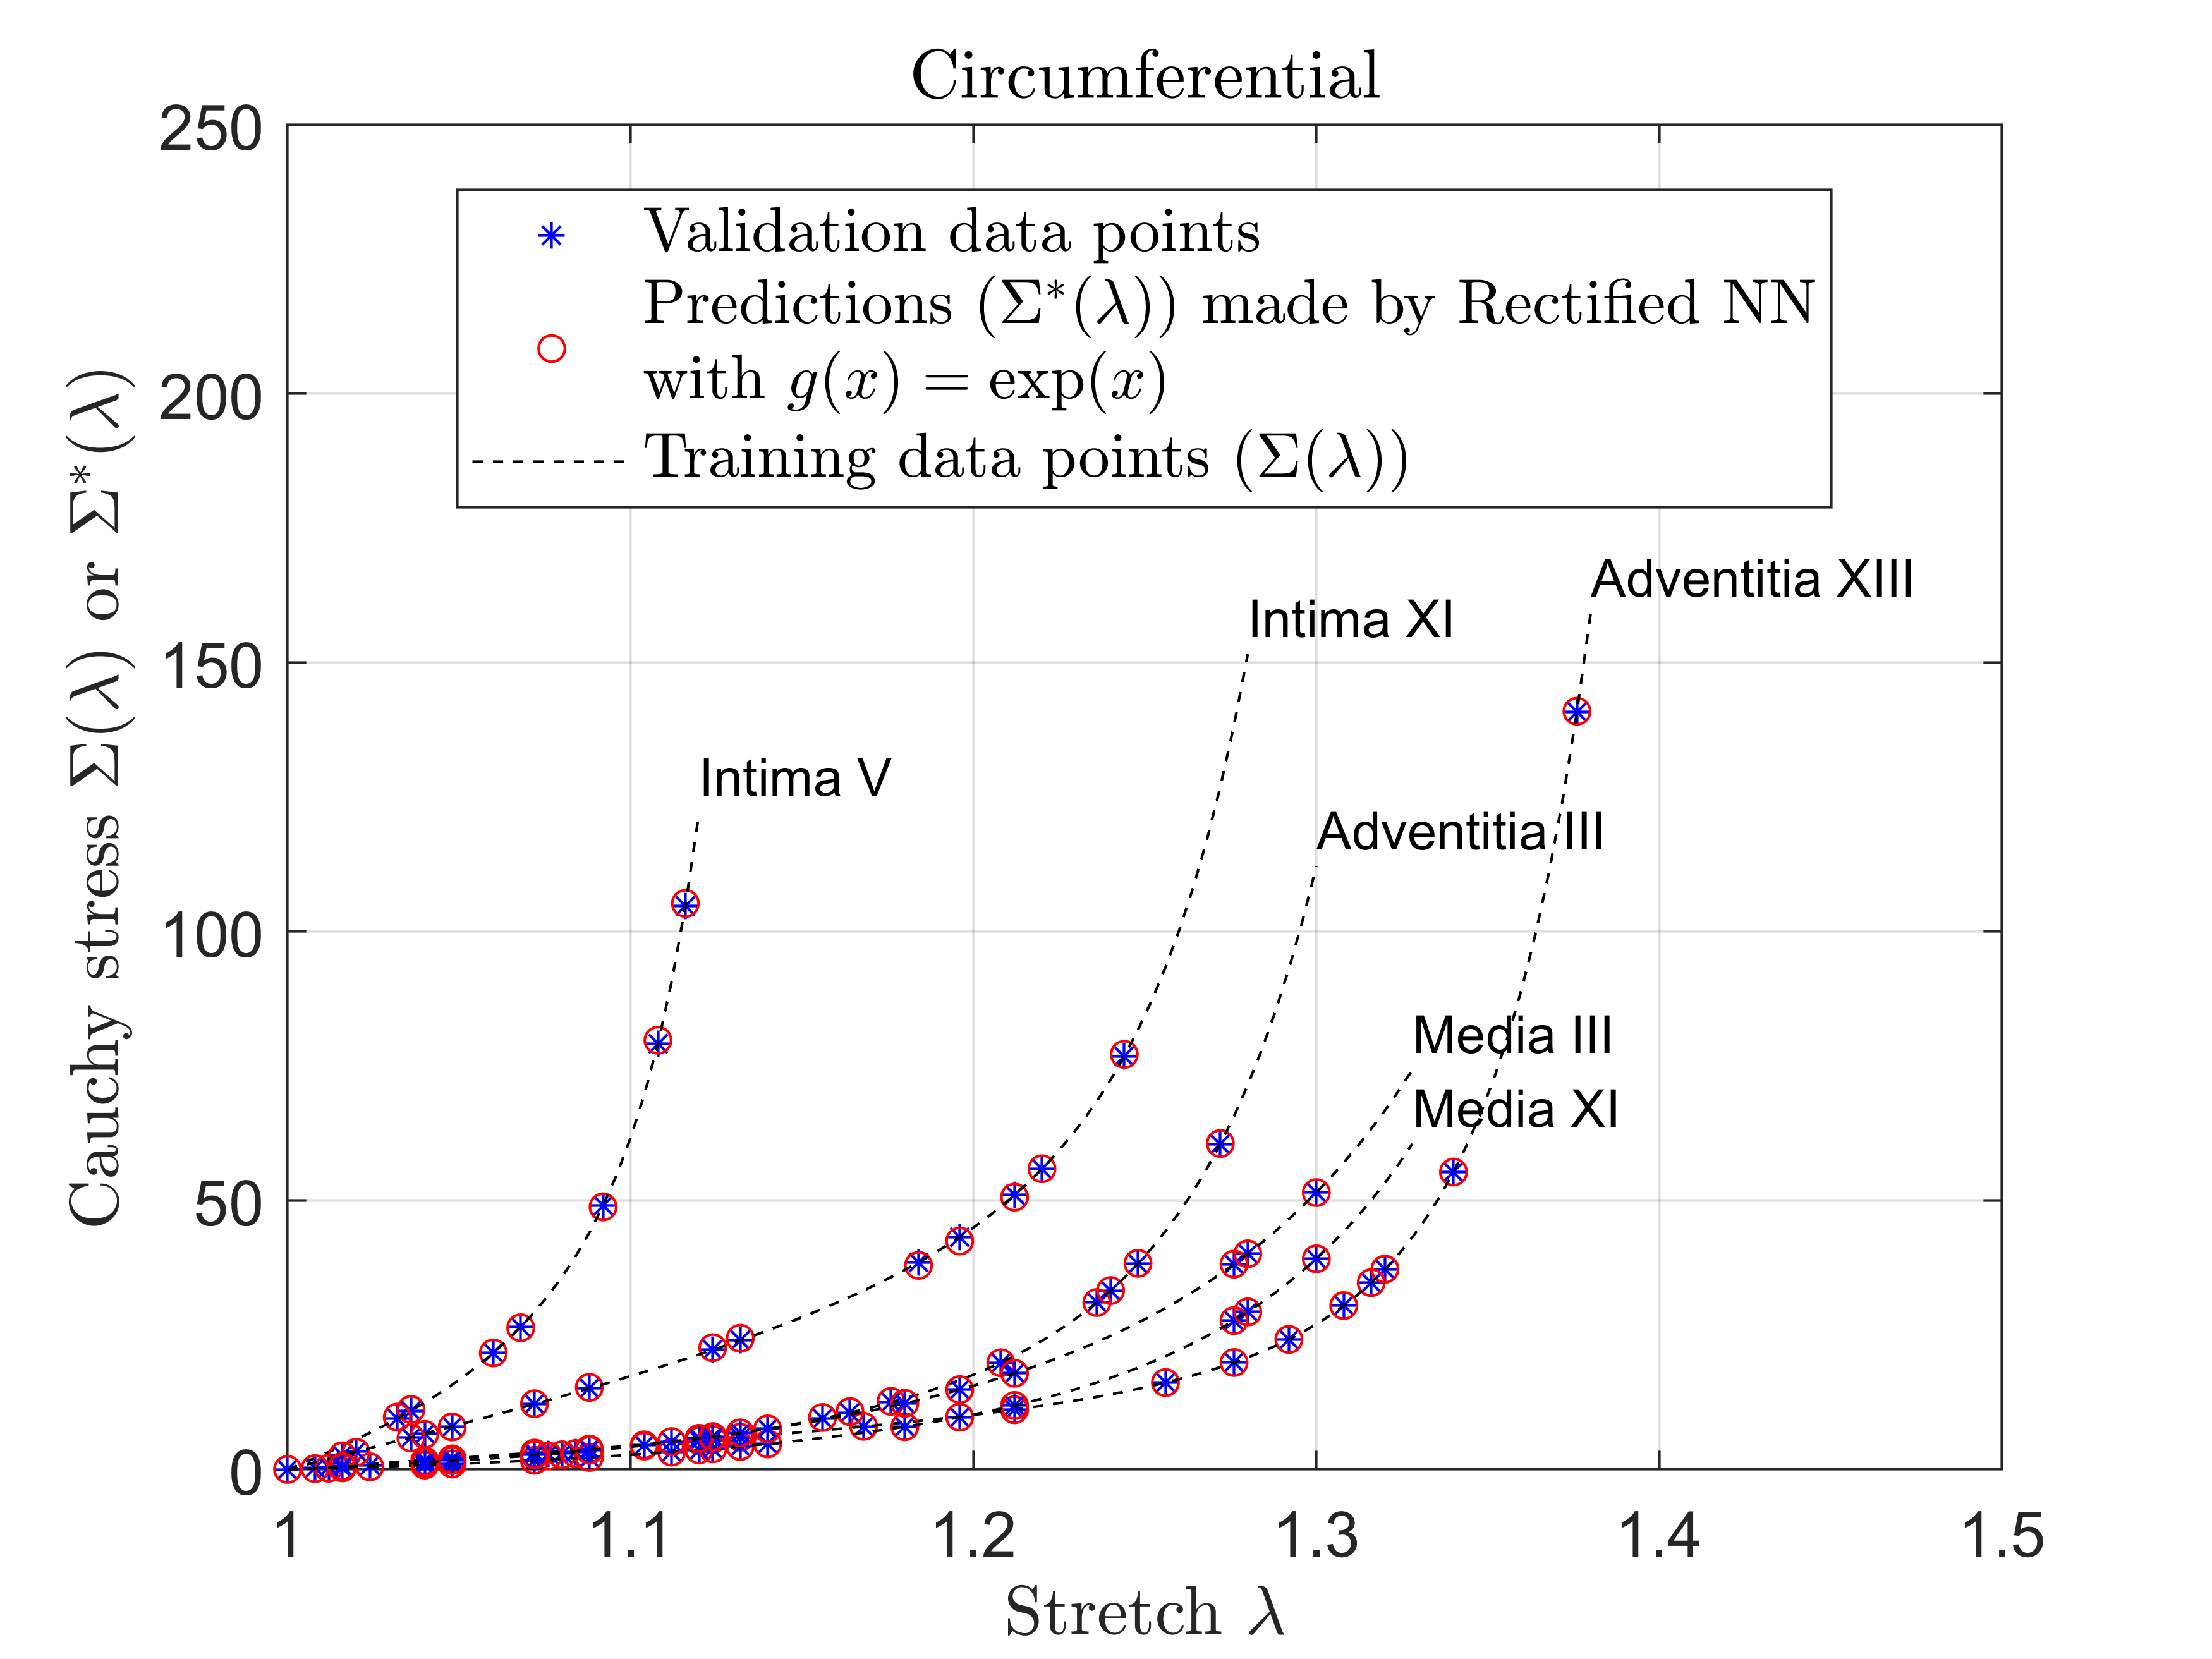
\includegraphics[width=0.5\textwidth]{Pictures/circ.png}
    \end{center}
    \caption[Reference stress response and values, RNN predictions (circumferential).]{Reference stress response $\lambda \mapsto \Sigma(\lambda)$ (black dashed line), reference values (blue star), and rectified neural network predictions (red circle) for the validation dataset in the circumferential direction (six experimental responses are considered for illustration purposes).}
    \label{fig:exp_circ}
\end{figure}
\begin{figure}[ht!]
    \begin{center}
        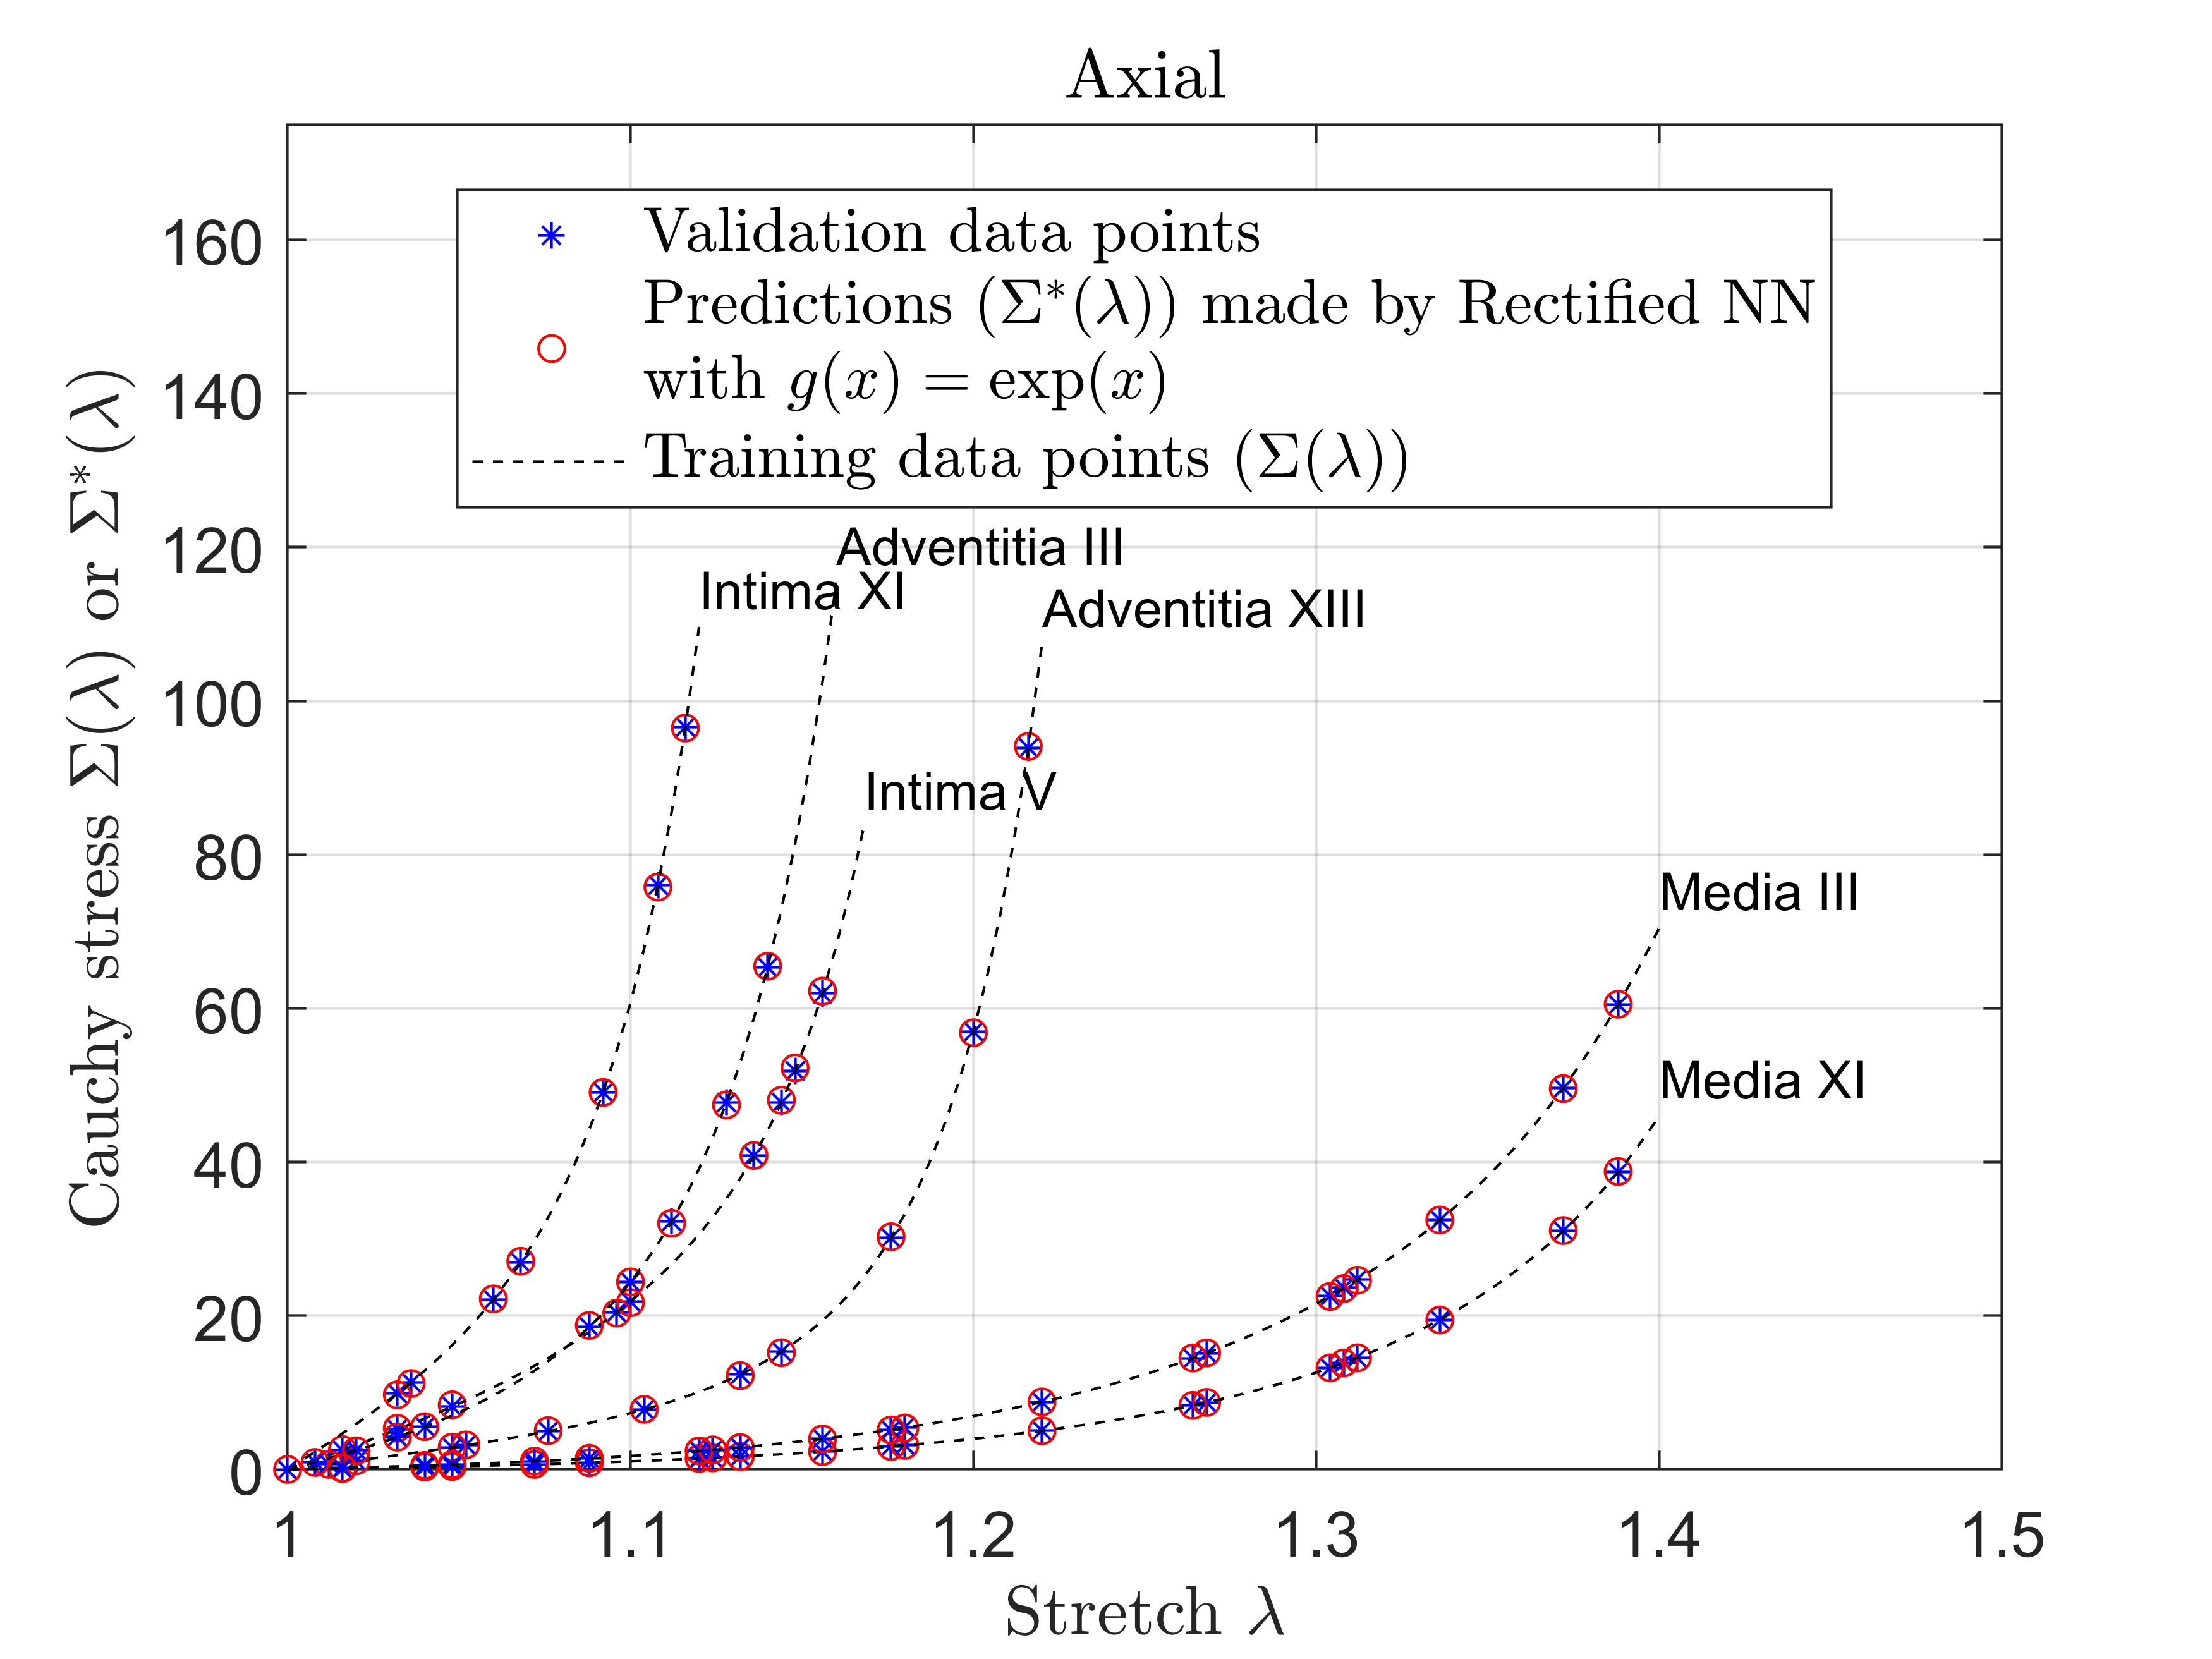
\includegraphics[width=0.5\textwidth]{Pictures/axial.png}
    \end{center}
    \caption[Reference stress response and reference values, RNN predictions (axial).]{Reference stress response $\lambda \mapsto \Sigma(\lambda)$ (black dashed line), reference values (blue star), and rectified neural network predictions (red circle) for the validation dataset in the axial direction (six experimental responses are considered for illustration purposes).}
    \label{fig:exp_axial}
\end{figure}
With a maximal validation error equal to $1.0096\times10^{-4}$ (obtained for sample \#XI, intima layer), it is seen that the rectified neural network can reproduce the experimental data very well, for all different layers in the two directions.

\begin{table}[ht!]
\caption[Validation errors for each sample.]{Validation errors for each sample. Specimen numbers are those reported in \cite{holzapfel2005determination}.}
\label{tab:val-err}
\begin{center}
    \begin{tabular}{|c|c|} 
 \hline
 Layer/Specimen number & Error $\mathcal{L}_d$ $\times 10^{-4}$ \\
 \hline
 Adventitia/\#III & 0.9972 \\
 Adventitia/\#XIII & 0.1331 \\
 Intima/\#V & 0.7994 \\
 Intima/\#XI & 1.0096 \\
 Media/\#III & 0.0252 \\
 Media/\#XI & 0.0355 \\
 \hline
\end{tabular}
\end{center}

\end{table}

\chapter{A Nonlinear-Manifold Reduced-Order Model and Operator Learning for Partial Differential Equations with Sharp Solution Gradients}
\label{chap:cnnae}

In spite of its many successes, the linear subspace solution representation suffers from the inability to represent certain physical simulation solutions with a small basis dimension, such as advection-dominated problems whose solutions possess large spatial gradients. This is because linear subspace can only retain a small dimensionality for problems with a fast decaying Kolmogorov $n$-width, i.e., the solution can be well-represented by a small number of basis functions. Problems with a slowly decaying Kolmogorov $n$-width include, but are not limited to, the hyperbolic equations with high Reynolds number, the Boltzmann transport equations, and the traffic flow simulations. As one way to alleviate such issue, there have been many attempts to replace the linear subspace solution representation with nonlinear manifolds (see also \cite{BARNETT2023112420} for another closure strategy). Recently, a physics-informed NM-ROM was proposed in \cite{kim2022fast}, where a shallow masked autoencoder and hyper-reduction techniques are used to achieve a speed-up of the NM-ROM compared to the corresponding FOM. However, results provided by standard DNN-based NM-ROM remain hard to analyze beyond accuracy evaluation, due to the lack of interpretability in deep learning models. As a result, it is difficult to determine the structure and parameters of the DNNs a priori, and a huge amount of effort has to be made to tune the NM-ROMs to achieve good performance. 

In this work, we devise a novel structure for the decoder in the NM-ROM, such that the underlying nonlinear mapping closely resembles the formulation of adaptive basis methods. In essence, the non-linearity in the proposed NM-ROM is introduced through a DNN in the smoothing kernels. The nonlinear manifolds suggested by the trained NM-ROM allows one to gain additional insight into the nonlinearities of the corresponding FOM. We also propose a DNN-based reduced operator inference that learns from the latent space for full models based on time-dependent partial differential equations. Note that the issue of learning operators associated with ordinary and partial differential equations (in physical or latent spaces) has attracted much attention over the last decade. Providing an exhaustive review on --- and a fair numerical comparison between --- all existing approaches is outside the scope of the present work (if at all possible); see \cite{lu2021learning,li2020fourier, li2022fourier,wen2022u,lu2021deepxde,pang2019fpinns,zhang2019quantifying,li2020multipole,li2020neural,tran2021factorized,guibas2021adaptive,tripura2022wavelet,gupta2021multiwavelet,kovachki2021neural,jin2022mionet,li2021physics,raonic2023convolutional,batlle2023kernel} to list a few, as well as \cite{LU2022114778,kovachki2023neural} for comparisons between some operator learning techniques (see Section 5.1 in \cite{LU2022114778} and Section 7.2.2 in \cite{kovachki2023neural}, in particular, for results on a one-dimensional Burgers' equation in a diffusion-dominated regime). Note that the above frameworks typically perform on fixed spatial domains, under given boundary conditions. In this context, a framework to address transfer across domains and boundary conditions was proposed in \cite{WANG2022114424}. Finally, we discuss algorithmic issues for online computations and propose a strategy for vectorized implicit time integration. 

This section is organized as follows. The formulation is first presented in Section~\ref{sec:theory}. We introduce the initial boundary value problem (IBVP) in a generic form. We then review commonly employed autoencoders and derive the architecture for a convolutional neural network-based autoencoder with adaptive kernels. Next, we present operator learning strategies in the latent space, including the operator inference approach recently proposed in \cite{qian2022reduced} and the DNN-based approach. We also provide an algorithm for enhanced implicit time integration. Application to a 2D Burgers' equation in an advection-dominated regime is subsequently presented in Section~\ref{sec:example}. Convergence in training cost and accuracy for both the autoencoders and operator inference is specifically discussed. The performance of the vectorized implicit time integration is also assessed on various GPUs.

\section{Nomenclature}

We use the following nomenclature/abbreviation for various autoencoders throughout this section:
\begin{itemize}
    \item LAE: linear autoencoder
    \item  POD: proper orthogonal decomposition
    \item NAE: nonlinear autoencoder
    \item DAE: nonlinear deep autoencoder
    \item LE-DAE: nonlinear deep autoencoder with linear encoder
    \item NE-DAE: nonlinear deep autoencoder with nonlinear encoder
    \item SAE: nonlinear sparse autoencoder
    \item LE-SAE: nonlinear sparse autoencoder with linear encoder
    \item NE-SAE: nonlinear sparse autoencoder with nonlinear decoder
    \item CNNAE: nonlinear convolutional autoencoder
    \item LE-CNNAE: nonlinear convolutional autoencoder with linear encoder
    \item NE-CNNAE: nonlinear convolutional autoencoder with nonlinear encoder
    
\end{itemize}
The above autoencoders form a hierarchy that is depicted in \ref{fig: summary of autoencoders}. 
\begin{figure}[!htb]
    \begin{center}
        \includegraphics[trim = {5cm 7cm 5cm 7cm}, clip, width=\textwidth]{Hierarchy.pdf}
    \end{center}
    \caption[Hierarchy of several autoencoders.]{The figure shows the hierarchy of several autoencoders. This paper contributes to the development of CNNAE that achieve both speedup and accuracy with the NM-ROM (following the path highlighted in blue). Throughout the paper, we will compare the performance of LAE and NAEs.}
    \label{fig: summary of autoencoders}
\end{figure}
Two non-intrusive operator inference techniques are used to solve the reduced-order formulation in this work, namely
\begin{itemize}
    \item OpInf (quadratic operator inference) and 
    \item DNNOp (deep-neural-network-based operator learning).
\end{itemize}
Autoencoders were implemented in JAX, while operator learning techniques were developed in PyTorch. The main symbols used in this paper are provided in Tab.~\ref{tab:symbols}.

\begin{table}[!ht]
    \caption[List of main symbols.]{List of main symbols.}
\label{tab:symbols}
\begin{center}
    \begin{tabular}{cc}
        \hline
        Symbol& Description\\\hline
        $\Omega$& Bounded domain in $\mathbb{R}^{d}$ with smooth boundary $\partial\Omega$\\
        $u$ & $d$-dimensional physical state \\
        $u_0$& Initial condition, $u_0(\cdot) = u(\cdot, t_0)$\\
        $f$& Spatial differential operator\\
        $\mathcal{U}$ and $\mathcal{U}_0$& Function spaces for $u$ and $u_0$\\
        $\mathcal{U}^r$ and $\mathcal{U}^r_0$& Reduced latent spaces associated with $\mathcal{U}$ and $\mathcal{U}_0$\\
        $\mathcal{G}^\dagger$& Flow map operator from $\mathcal{U}_0$ to $\mathcal{U}$\\
        $\mathcal{H}$& Flow map operator from $\mathcal{U}^r_0$ to $\mathcal{U}^r$\\
        $E$& Encoder from $\mathcal{U}$ to $\mathcal{U}^r$\\
        $D$& Decoder from $\mathcal{U}^r$ to $\mathcal{U}$\\
        $\btu^{\left<m\right>}(u_0^{(\ell)})$& Discretized solution vector for initial condition $u_0^{(\ell)}$ at $m$-th time step\\
        $\hat{\btu}^{\left<m\right>}(u_0^{(\ell)})$& Latent solution vector for initial condition $u_0^{(\ell)}$ at $m$-th time step\\
        $\tilde{\btu}^{\left<m\right>}(u_0^{(\ell)})$& Approximated solution vector for initial condition $u_0^{(\ell)}$ at $m$-th time step\\
        $\dot{\hat{\btu}}^{\left<m\right>}(u_0^{(\ell)})$& Time derivative of the latent solution vector $\hat{\btu}^{\left<m\right>}(u_0^{(\ell)})$\\
        \hline
    \end{tabular}
\end{center}
\end{table}

\section{Theory}
\label{sec:theory}

\subsection{Problem Statement}
We consider the initial boundary value problem 
\begin{subequations}\label{eq:ibvp}
    \begin{align}
        \frac{\partial u}{\partial t} & = f(u) \quad~ \text{in } \Omega \times (t_0, t_f]\,,\\
        u(x, t_0) & = u_0(x) \quad \text{on } \Omega\,,
    \end{align}
\end{subequations}
where $u: \Omega \times (0, t_f] \to \mathbb{R}^{d}$ is the unknown $d$-dimensional physical state, $f$ is a spatial differential operator, $\Omega$ is a bounded domain in $\mathbb{R}^{d}$ with smooth boundary $\partial\Omega$, $(0, t_f]$ denotes the time interval of interest, and $u_0: \Omega \to \mathbb{R}^{d}$ is the initial condition. The solution $u$ and initial condition $u_0$ are assumed to belong to \textit{ad hoc} (separable Hilbert) function spaces, denoted by $\mathcal{U}$ and $\mathcal{U}_0$, respectively. Eq.~\eqref{eq:ibvp} is referred to as the full-order model (FOM). 

In this work, we seek to approximate the flow map operator $\mathcal{G}^\dagger: \mathcal{U}_0 \to \mathcal{U}$ mapping the initial condition to the solution at time $t$. To this end, we introduce \textit{spatial} encoders for $\mathcal{U}_0$ and $\mathcal{U}$, denoted by $E_0$ and $E$, respectively. Similarly, $D_0$ and $D$ are the associated spatial decoders such that $D_0 \circ E_0 \approx I_0$ and $D \circ E \approx I$, where $I_0$ and $I$ are the identity operators in $\mathcal{U}_0$ and $\mathcal{U}$, respectively. We further introduce the \textit{operator} $\mathcal{H}$ approximating the flow map between the latent spaces $\mathcal{U}_0^{r_0}$ and $\mathcal{U}^r$ (in time domain). The construction of the surrogate operator then proceeds with the definition of $E_0$, $D$, and $\mathcal{H}$ such that $\mathcal{G} = D \circ \mathcal{H} \circ E_0$ is an accurate approximation to $\mathcal{G}^\dagger$; see Fig.~\ref{fig:maptomap}.
\begin{figure}[!ht]
	\begin{center}
        \includegraphics[trim = {10cm 9.5cm 10cm 9.25cm}, clip, width=0.5\textwidth]{Fig-MaptoMap.pdf}
    \end{center}
    \caption[Flow map $u_0 \mapsto u(\cdot, t)$, $t > 0$.]{Mappings used to approximate the flow map $u_0 \mapsto u(\cdot, t)$, $t > 0$ (inspired by \cite{stuart2021}).}
    \label{fig:maptomap}
\end{figure}
The definition of the encoder $E_0$ and decoder $D$ is first addressed in Section~\ref{sec: autoencoders}. A \textit{non-exhaustive} list of possible strategies for operator learning is then presented in Section~\ref{sec: operators}. 

\subsection{Autoencoders}\label{sec: autoencoders}
Consider a spatial discretization of $\Omega$, defined by a collection of points $\{\btx_i\}_{i = 1}^{N_s}$, and a time discretization $\{t_m = m \Delta t\}_{m = 0}^{N_t}$ of the time interval $[0,t_f]$, with $\Delta t$ the step size and $t_f = N_t \Delta t$. For a given initial condition $u_0^{(\ell)}$, $1 \leq \ell \leq N_{ic}$ and $1 \leq m \leq N_t$, let 
$$\btu^{\left<0\right>}(u_0^{(\ell)}) = (u_0(\btx_1; u_0^{(\ell)})^T, \ldots, u_0(\btx_{N_s}; u_0^{(\ell)})^T)^T$$
and denote by
$$\btu^{\left<m\right>}(u_0^{(\ell)}) = (u(\btx_1, t_m; u_0^{(\ell)})^T, \ldots, u(\btx_{N_s}, t_m; u_0^{(\ell)})^T)^T$$
the vector in $\mathbb{R}^N$ (with $N = d N_s$) containing the solution at all points at the $m$th time step. Consider the mean over all time steps and initial conditions:
\begin{align}
    \bar{\btu} = \frac{1}{N_{snp}} \sum_{\ell = 1}^{N_{ic}} \sum_{m = 0}^{N_t} \btu^{\left<m\right>}(u_0^{(\ell)})\,,
\end{align}
with $N_{snp}=N_{ic}(N_t + 1)$. We then introduce the matrix of solution snapshots $\btU \in \mathbb{R}^{N \times N_{snp}}$ as
\begin{align}\label{eq:snapshot-matrix}
    \btU = [\btu^{\left<0\right>}(u_0^{(1)}) - \bar{\btu}, \ldots, \btu^{\left<N_t\right>}(u_0^{(1)}) - \bar{\btu}, \ldots, \btu^{\left<0\right>}(u_0^{(N_{ic})}) - \bar{\btu}, \ldots, \btu^{\left<N_t\right>}(u_0^{(N_{ic})}) - \bar{\btu}]\,.
\end{align}
It what follows, we discuss various strategies to construct $E$ and $D$, and use $E$ to encode in $\mathcal{U}_0$ (i.e., we take $E_0 = E$ and $r_0 = r$). Note that this choice is generally acceptable since the solution $u$ typically exhibits less regularity than $u_0$, and becomes licit for encoding-decoding approaches involving function bases (e.g., for the POD approach in Section \ref{sec: lsrom}). We let $\hat{u}(t) = E(u(x,t))$ and $\tilde{u}(x,t) = D(\hat{u}(t)) = D(E(u(x,t)))$, with $\tilde{u} \approx u$, and carry this convention over all forms of representation without adjusting notation for operators, for ease of presentation (i.e., we consider $\hat{\btu}^{\left<m\right>} = E(\btu^{\left<m\right>})$ and $\tilde{\btu}^{\left<m\right>} = D(\hat{\btu}^{\left<m\right>})$ after discretization). 

Classical autoencoders are reviewed below as a baseline for comparison (see Sections \ref{sec: lsrom}, \ref{sec: shallow autoencoder}, and \ref{sec: sae}), and a new decoding strategy, inspired by adaptive basis methods, is proposed (see Section \ref{sec: cnnae}). Note that for nonlinear reduction techniques involving neural networks, hidden layers with or without nonlinear activation functions (here, the swish activation function $a$ defined as $a(x) = x/(1+\exp(-x))$) are considered. Such architectures are identified with the prefixes ``NE'' and ''LE'', respectively. Activation functions are used in the hidden layers in all nonlinear decoders (except for the output layer). 

\subsubsection{POD Autoencoder}\label{sec: lsrom}
The Proper Orthogonal Decomposition (POD) is arguably the most widely used linear approach to encode and decode in high-dimensional state spaces, due to its amenability for analysis and ease of use. In this method, the encoder $E: \mathbb{R}^N \to \mathbb{R}^r$, $r \ll N$, is given by 
\begin{align}
    \hat{\btu}^{\left<m\right>} = E(\btu^{\left<m\right>}) = (\inner{\mathbb{R}^N}{\btu^{\left<m\right>}}{\btphi_1}, \ldots, \inner{\mathbb{R}^N}{\btu^{\left<m\right>}}{\btphi_r})^T\,,
\end{align}
where $\inner{\mathbb{R}^N}{\cdot}{\cdot}$ is the standard Euclidean inner product in $\mathbb{R}^N$ and $\btphi_1, \ldots, \btphi_r$ are the left singular vectors associated with the largest singular values in the singular value decomposition of the snapshot matrix (see Eq.~\eqref{eq:snapshot-matrix}):
\begin{align}
    \btU = \btPhi \boldsymbol{\Sigma} \btV^T\,,
\end{align}
where $\btPhi = [\btphi_1, \ldots, \btphi_{N}] \in \mathbb{R}^{N \times N}$ and $\btV \in \mathbb{R}^{N_{snp} \times N_{snp}}$ are real orthogonal matrices, and $\boldsymbol{\Sigma} \in \mathbb{R}^{N \times N_{snp}}$ is the matrix containing the singular values (ranked in non-increasing order) on the diagonal. The decoder $D:\mathbb{R}^r \to \mathbb{R}^N$ then defines the approximation in the span of the POD modes $\btphi_1, \ldots, \btphi_r$:
\begin{align}
    \tilde{\btu}^{\left<m\right>} &= \sum_{i=1}^r \inner{\mathbb{R}^N}{\btu^{\left<m\right>}}{\btphi_i} \btphi_i\,.
\end{align}
The above formulation is optimal in the $L^2$ sense in terms of projection error, for a given reduced dimension $r$. The advantages and limitations of this method are well established. In particular, the POD-based approach can be used to significantly accelerate simulations when the solution space of the discretized system exhibits a fast decaying Kolmogorov $n$-width, but struggles to achieve speed-ups in highly nonlinear problems, the solutions to which have large gradients. Strategies to address the irreducibility issue can be found in \cite{BARNETT2023112420} and the references therein, for instance.

\subsubsection{Deep Autoencoder}\label{sec: shallow autoencoder}
We first consider a simple Deep Autoencoder (DAE), defined through a composite mapping with fully connected layers:
\begin{align}
    E = E^{(n_e)} \circ E^{(n_e -1)} \circ \ldots \circ E^{(1)}\,, 
\end{align}
where $n_e$ denotes the number of layers in the encoder. As previously indicated, we denote by NE-DAE and LE-DAE the encoder with or without activation functions, respectively. In the former case, each hidden layer is defined as
\begin{align}
    E^{(i)}(\btx) = a(\btW_e^{(i)} \btx + \btb_e^{(i)})\,, \quad i < n_e\,,
\end{align}
where $\btW_e^{(i)} \in \mathbb{R}^{p \times q}$ and $\btb_e^{(i)} \in \mathbb{R}^{p}$ are the matrix of weights and vector of biases in the $i$th layer with input dimension $q$ and output dimension $p$, respectively, and the swish activation function acts component-wise. For LE-DAE, the above equation becomes
\begin{align}\label{eq: hidden layer}
    E^{(i)}(\btx) = \btW_e^{(i)} \btx + \btb_e^{(i)}\,,\quad i < n_e\,,
\end{align}
and $E$ can be reduced to a single-layer neural network. The decoder in both DAEs is defined as
\begin{align}
    D = D^{(n_d)} \circ D^{(n_d -1)} \circ \ldots \circ D^{(1)}\,,
\end{align}
where $n_d$ is the number of layers in the decoder and
\begin{align}
    D^{(i)}(\btx) & = 
    \begin{cases} 
        \btW_d^{(i)} x + \btb_d^{(i)}, & i = n_d\,,\\
        a(\btW_d^{(i)} x + \btb_d^{(i)}), & i < n_d\,.
    \end{cases}
\end{align}
The DAE is trained by minimizing the classical mean squared loss function
\begin{align}\label{eq: mse}
    l^{\text{mse}}_{\text{DAE}}(\boldsymbol{\Theta}_e, \boldsymbol{\Theta}_d) = \frac{1}{N_{snp}} \sum_{\ell = 1}^{N_{ic}} \sum_{m=0}^{N_t}\norm{\btu^{\left<m\right>}(u_0^{(\ell)}) - \bar{\btu} - D(E(\btu^{\left<m\right>}(u_0^{(\ell)})-\bar{\btu}; \boldsymbol{\Theta}_e); \boldsymbol{\Theta}_d)}^2\,,
\end{align}
where $\boldsymbol{\Theta}_e$ and $\boldsymbol{\Theta}_d$ contain all trainable parameters in the encoder and decoder, respectively.

\subsubsection{Sparse Autoencoder}\label{sec: sae}
One approach to reduce the computational cost and increase the efficiency of the autoencoder is to use sparse neural networks---a type of neural network that utilizes only a fraction of the available connections between neurons. By reducing the number of parameters needed to train a model, such models can lead to faster convergence rate and reduced memory requirements. In addition, sparse neural networks can improve model interpretability by highlighting the most relevant features and reducing the noise caused by irrelevant connections. These benefits make sparse neural networks an attractive option for applications with limited computational resources and/or where model interpretability is important. 

In \cite{kim2022fast}, a Sparse Autoencoder (SAE) with a special sparsity pattern in the nonlinear decoder was proposed. Such a sparsity pattern mimics that of a diffusion operator in numerical discretization methods, such as the finite difference method (FDM). A masked autoencoder is introduced by adding a so-called mask matrix $\btS$ which contains either zero or one to create a sparsely connected layer for the decoder: 
\begin{align}\label{eq: shallow mask}
    \btS = \heaviside(\btC \btB)\,, \quad \btB = \sum_i \sum_j b_{ij} \bte_i \bte_j\,, \quad b_{ij} = \begin{cases}
        1\,, \quad i \delta \leq j \leq i \delta + b\,, \\
        0\,, \quad \text{otherwise}\,,
    \end{cases}
\end{align}
where $\btC \in \mathbb{R}^{N \times N}$ is the nodal connectivity matrix (e.g., in the FDM), $\{\bte_i\}_{i = 1}^N$ are one-hot vectors in $\mathbb{R}^N$, $b$ is the bandwidth of the sparsity, and $\delta = \lfloor (M - b) / (N - 1) \rfloor$ is the average shift per neuron, where $M$ is the size of the last hidden layer in the sparse decoder. A sparse weight matrix is then obtained using the Hadamard (element-wise) product:
\begin{align}
    \btW^{(n_d)} = \btW^{(n_d)}_{\text{dense}} \odot \btS\,,
\end{align}
so that the mask is only applied at the last hidden layer of the decoder. Fig.~\ref{fig: S,C,B} shows an example of the mask matrix $\btS$, the nodal connectivity matrix $\btC$, and the base matrix $\btB$ for a 2D problem with $N = 16$, $M = 81$, $b = 6$, and $\delta b = 5$.
\begin{figure}[!htb]
  \begin{center}
    \begin{subfigure}[b]{0.4\textwidth}
        \begin{center}
            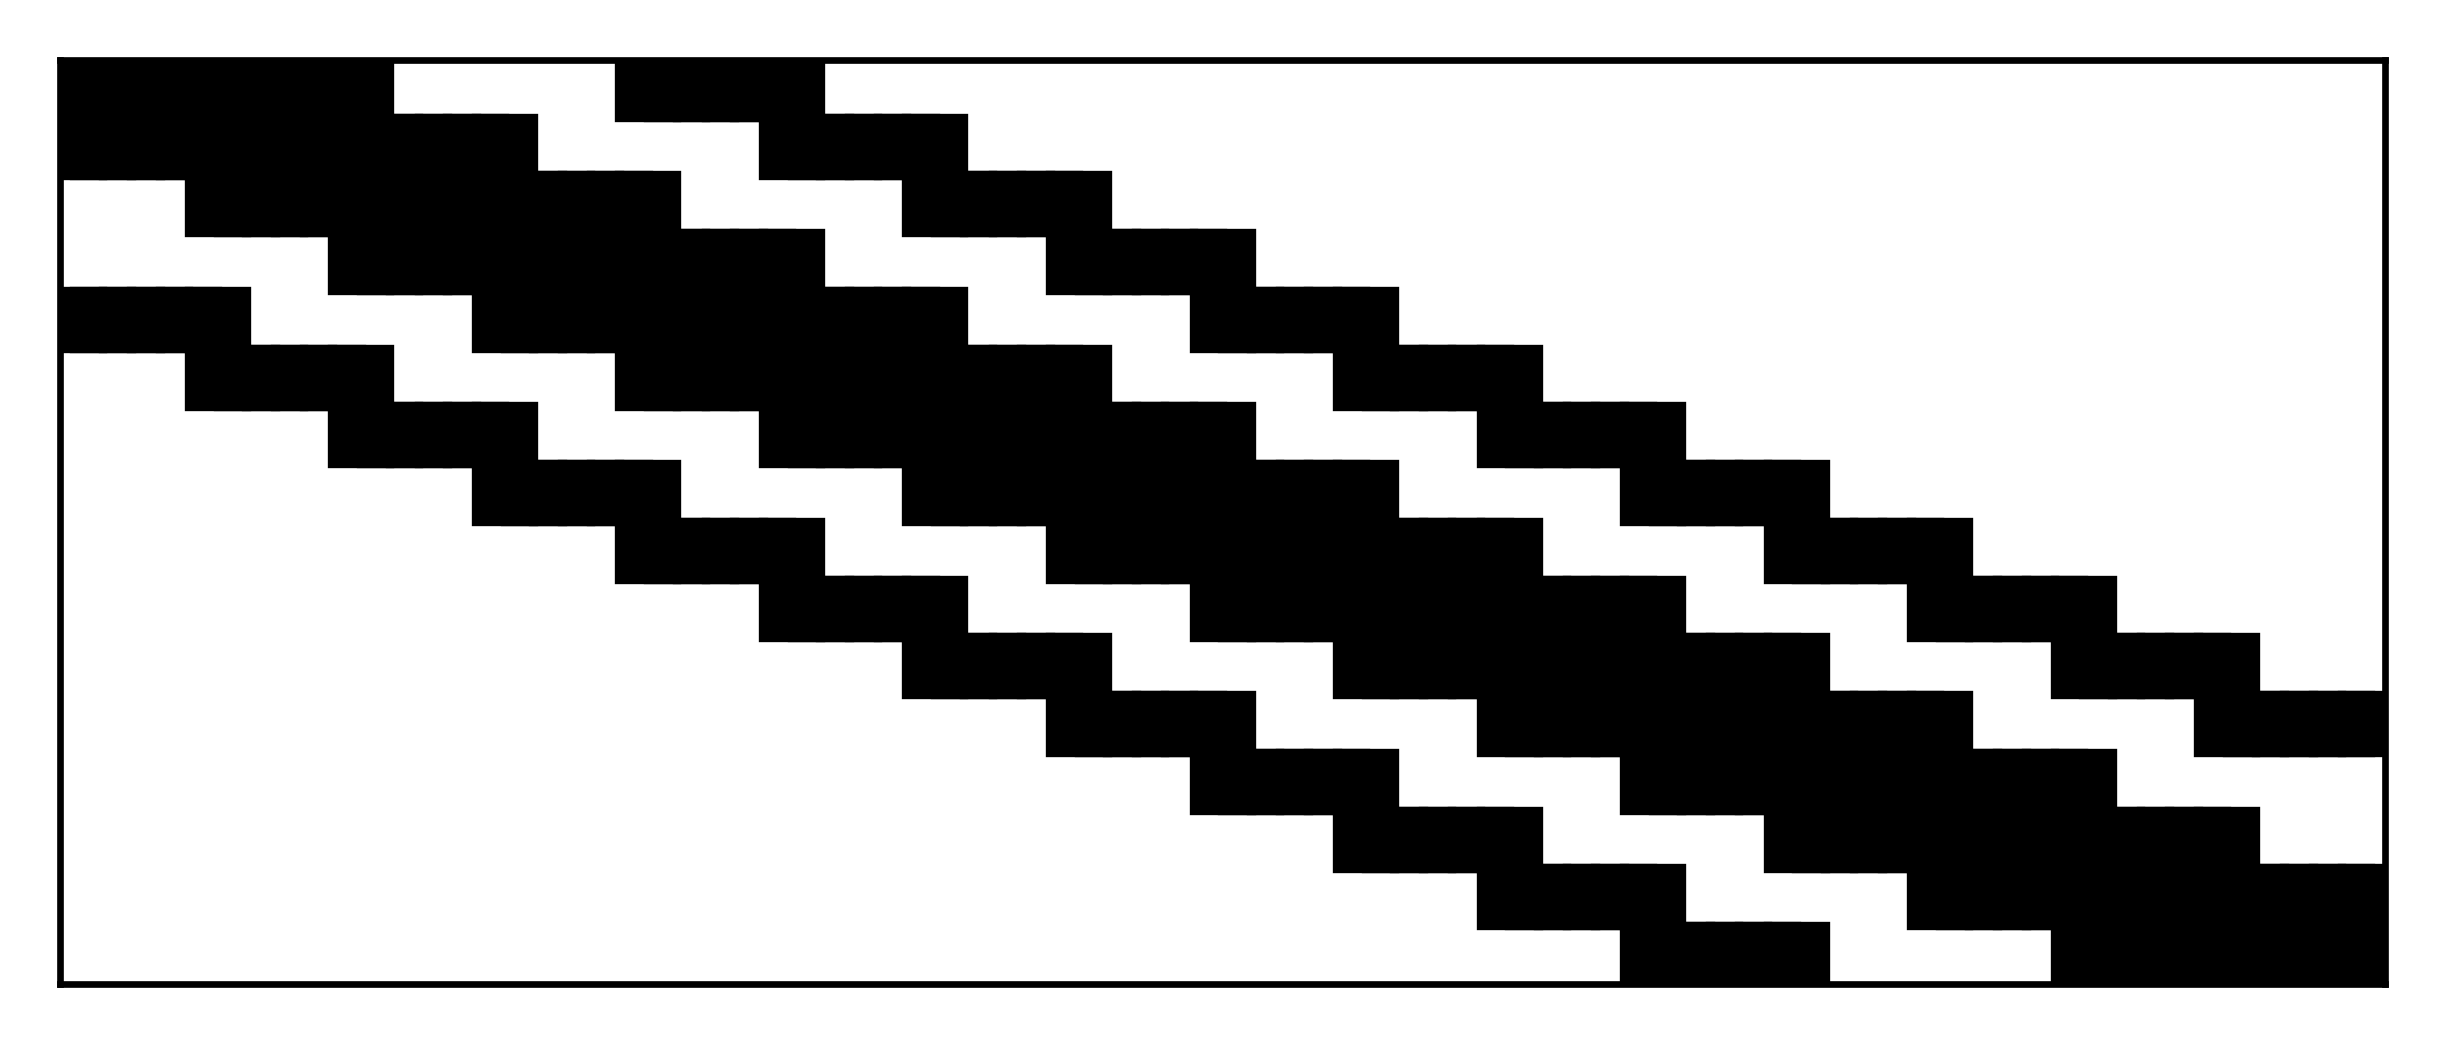
\includegraphics[width=\textwidth]{S.png}
        \end{center}
        \caption{$\btS$}
      \end{subfigure}
      \begin{subfigure}[b]{0.172\textwidth}
        \begin{center}
            
\includegraphics[width=\textwidth]{C.png}
        \end{center}
        \caption{$\btC$}
      \end{subfigure}
      \begin{subfigure}[b]{0.4\textwidth}
        \begin{center}
            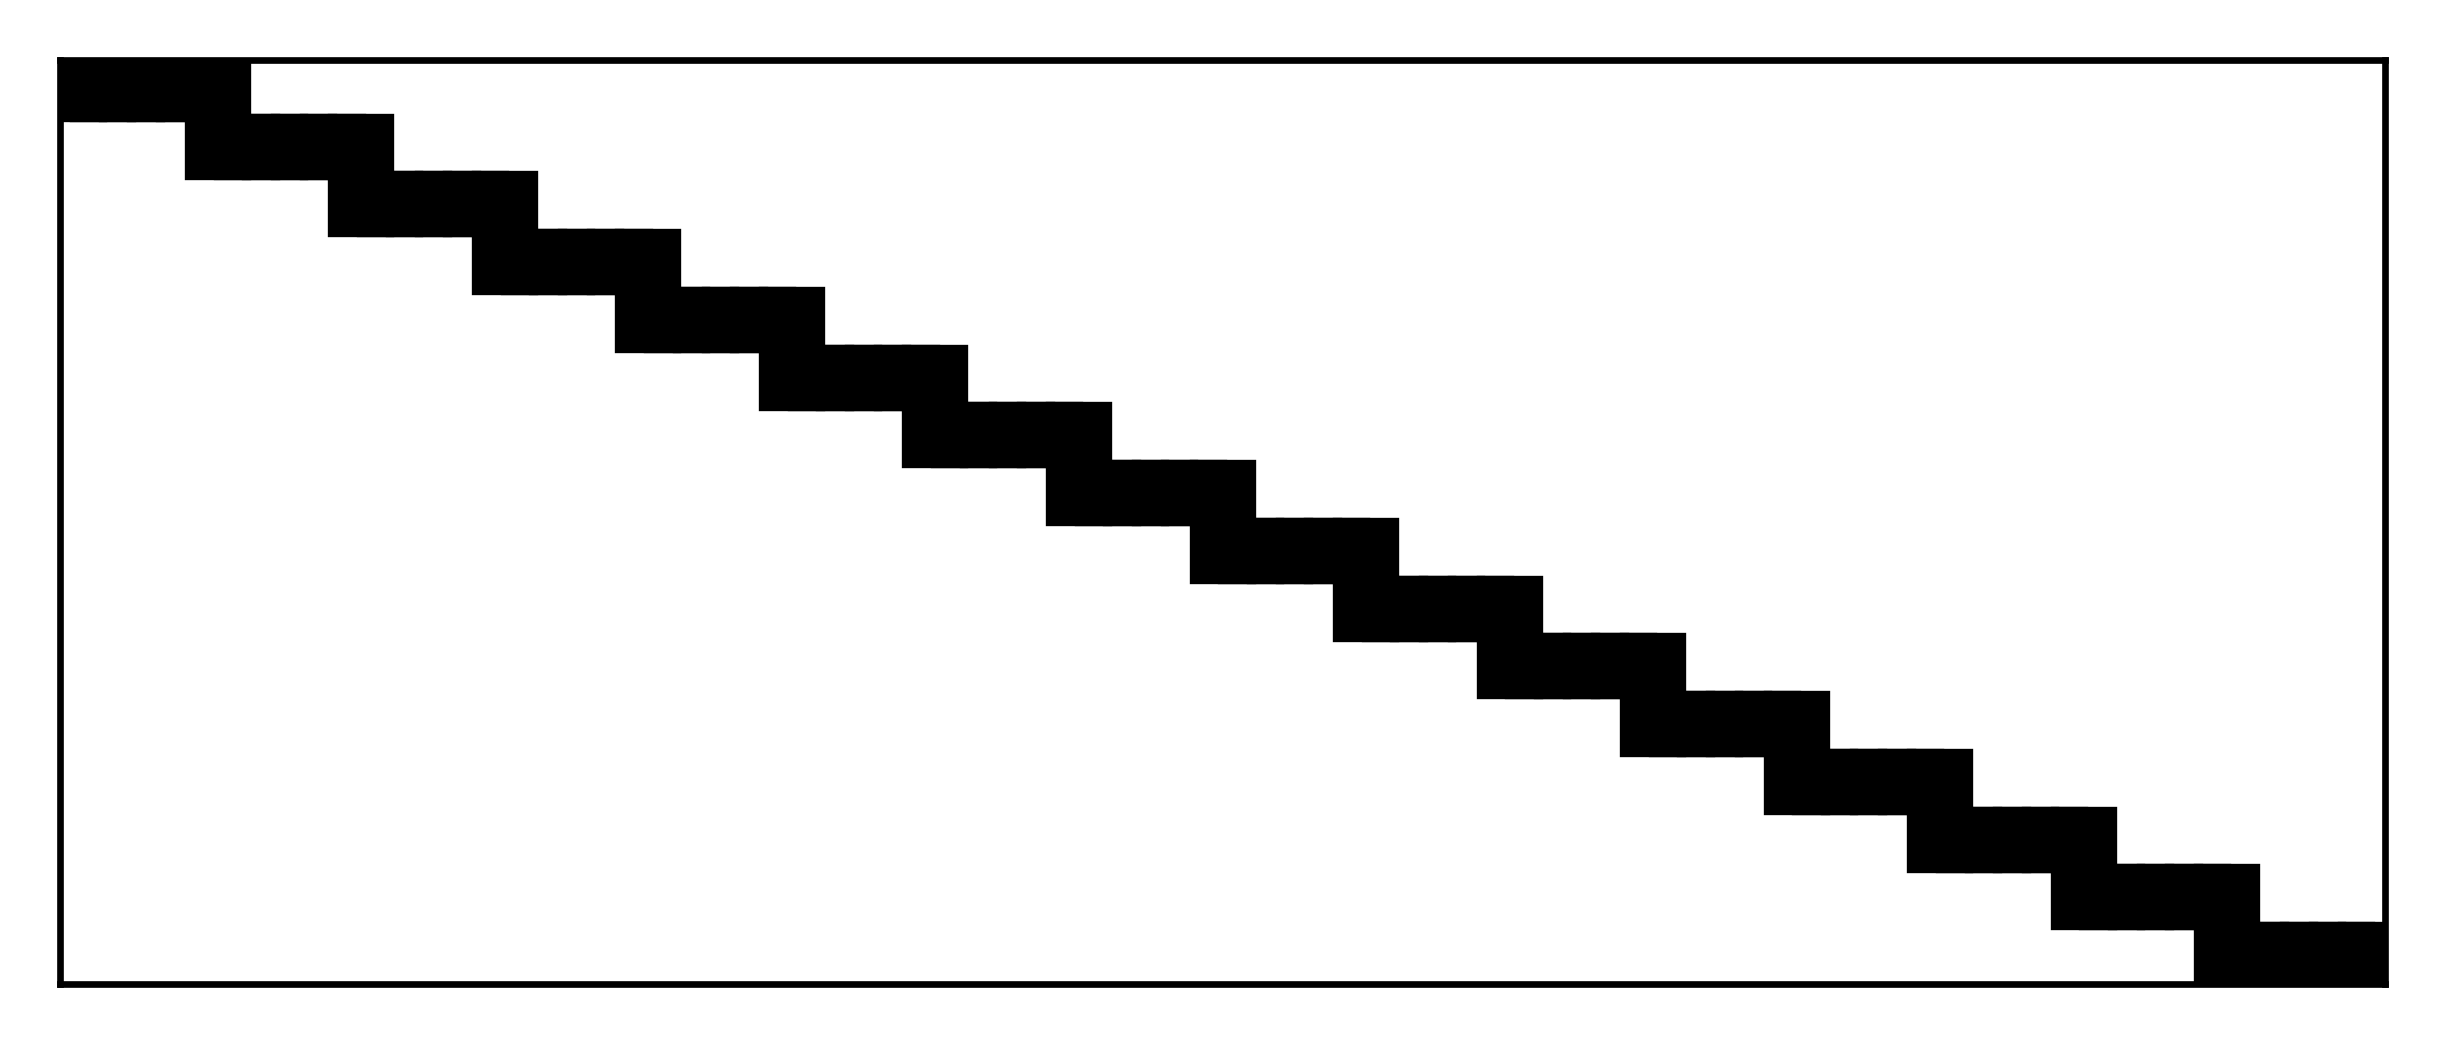
\includegraphics[width=\textwidth]{B.png}
        \end{center}
        \caption{$\btB$}
      \end{subfigure}
  \end{center}
  \caption[Mask matrix $\btS$, nodal connectivity matrix $\btC$, and base matrix $\btB$.]{Mask matrix $\btS$, nodal connectivity matrix $\btC$, and base matrix $\btB$ for $N = 16$, $M = 81$, $b = 6$, and $\delta b = 5$.}
  \label{fig: S,C,B}
\end{figure}

Following our convention, sparse autoencoders with or without activation functions in the encoder are denoted by NE-SAE and LE-SAE, respectively. 

\subsubsection{Convolutional Autoencoder with Enhanced Adaptivity}\label{sec: cnnae}

In this section, we propose to utilize Convolutional Neural Networks (CNNs) in the decoder to promote adaptivity. This choice is motivated by the fact that for PDEs with sharp solution gradients, the localization induced by convolutional filters helps extract local information from neighboring points, hence enabling high-quality reconstruction from the low-dimensional latent space $\mathcal{U}^r$. Our aim is to enhance adaptivity by considering trainable kernels in the convolution operator.

We define the decoder as
\begin{align} \label{eq: cnn decoder}
    D(\hat{\btu}^{\left<m\right>}) = \sum_{i=1}^r D_i(\hat{u}_i^{\left<m\right>}; \hat{\btu}^{\left<m\right>})\,,
\end{align}
where $D_i: \mathbb{R} \to \mathbb{R}^N$ is a lifting function defined as
\begin{align} \label{eq: cnn sub decoder}
    D_i(\hat{u}_i^{\left<m\right>}; \hat{\btu}^{\left<m\right>}) = (P \circ C_{\kappa_i}( \cdot\,; \hat{\btu}^{\left<m\right>}) \circ R \circ S_i)(\hat{u}_i^{\left<m\right>})\,,
\end{align}
where each term in the right-hand side is defined below.
\begin{itemize}
    \item The function $S_i$ is lifting $\hat{u}_i^{\left<m\right>}$ to a vector in $\mathbb{R}^N$ through the learnable mapping
    \begin{align}
    S_i(\hat{u}_i^{\left<m\right>}) = \btW_i \hat{u}_i^{\left<m\right>} + \btb_i\,,
    \end{align}
    where $\btW_i \in \mathbb{R}^N$ and $\btb_i \in \mathbb{R}^N$ are weights and bias of the fully connected layer.
    \item $R$ reshapes a vector in $\mathbb{R}^N$ into a matrix in $\mathbb{R}^{n_1 \times \ldots \times n_d}$, where $n_i$ specifies the number of degrees of freedom along the $i$th direction in the physical domain.
    \item The convolution function $C_{\kappa_i}:\mathbb{R}^{n_1 \times \ldots \times n_d} \to \mathbb{R}^{n_1 \times \ldots \times n_d}$ introduces adaptive spatial smoothing to capture localization. To define $C_{\kappa_i}$, we first introduce the kernel $\kappa_i:\mathbb{R}^r \to \mathbb{R}^{\mu^d}$ through the composite mapping
    \begin{align}
    \kappa_i = R_\kappa \circ ( K_i^{(n_k)} \circ K_i^{(n_k -1)} \circ ... \circ K_i^{(1)})\,,
    \end{align}
    where $K_i^{(n_k)} \circ K_i^{(n_k -1)} \circ ... \circ K_i^{(1)}$ is a neural network with $(n_k-1)$ hidden layers (with activation functions), i.e.,
    \begin{align}
    K_i^{(\ell)}(\btx) &= 
    \begin{cases} 
        \btW^{(\ell)}_i \btx + \btb^{(\ell)}_i\,, \quad \btW^{(\ell)}_i \in \mathbb{R}^{\mu^d \times q_{\ell - 1}}\,, \quad \btb^{(\ell)}_i \in \mathbb{R}^{\mu^d}\,,\quad \ell = n_k\,,\\
        a(\btW^{(\ell)}_i \btx + \btb^{(\ell)}_i)\,, \quad \btW^{(\ell)}_i \in \mathbb{R}^{p_\ell \times q_\ell} \,, \quad \btb^{(\ell)}_i \in \mathbb{R}^{p_\ell}\,, \quad \ell < n_k\,,
    \end{cases}
    \end{align}
    where $q_1 = r$ and the sets $\{p_\ell\}_{\ell = 1}^{n_k - 1}$ and $\{q_\ell\}_{\ell = 2}^{n_k - 1}$ are user-specified. The function $R_\kappa \in \mathbb{R}^{\mu^d} \mapsto \mathbb{R}^{\bigtimes_{j = 1}^d \mu}$ reshapes a vector into a matrix of size $\mu \times \ldots \times \mu $ ($d$ times). The function $C_{\kappa_i}$ then performs the discrete linear convolution of $(R \circ S_i)(\hat{u}_i^{\left<m\right>})$ with $\kappa_i(\hat{\btu}^{\left<m\right>})$.
    \item $P$ projects back from a matrix representation in $\mathbb{R}^{n_1 \times \ldots \times n_d}$ into a vector in $\mathbb{R}^N$.
\end{itemize}
In the above, and in contrast with strategies where the CNN is trained once for all, the trainable parameters in the kernel of the CNN are defined as the output of an auxiliary neural network and are, by construction, iteration-dependent: they evolve as a function of the latent solution vector to capture non-smoothness, hence promoting adaptivity.

The structure of the decoder $D$ is depicted in Fig.~\ref{fig: summary of cnnae}. 
\begin{figure}[!htb]
    \begin{center}
        \includegraphics[trim = {5.5cm 7cm 5.5cm 6.5cm}, clip, width = 0.8\linewidth]{FigSummaryCnnae.pdf}
    \end{center}
    \caption[General description of the CNN-based autoencoder.]{General description of the CNN-based autoencoder: $\btu^{\left<m\right>}$ is encoded into a latent vector $\hat{\btu}^{\left<m\right>}$ by the encoder. The latent vector is then decoded by the decoder to get $\tilde{\btu}^{\left<m\right>}$. A smoothing convolutional layer is added after the single dense layer at the beginning of the decoder to introduce nonlinearity into the decoder.}
    \label{fig: summary of cnnae}
\end{figure}
This convolutional autoencoder (denoted by CNNAE, with the LE-CNNAE and NE-CNNAE variations depending on whether activation functions are used in the encoder) is also trained by minimizing the mean squared loss given by Eq.~\eqref{eq: mse}.

\subsection{Strategies for Operator Learning Between Latent Spaces}\label{sec: operators}

We now turn to the construction of the surrogate operator $\mathcal{H}: \mathcal{U}_0^r \to \mathcal{U}^r$ mapping $\hat{\btu}_0 = E(u_0)$ to $\hat{\btu} = E(\btu)$. To this end, we consider the reduced-order model
\begin{equation}
    \frac{\partial \hat{\btu}(t)}{\partial t} = F(\hat{\btu}(t))\,, \quad \hat{\btu}(0) = \hat{\btu}_0\,,
\end{equation}
where the operator $F$ in the right-hand side is learned through an \textit{ad hoc} technique. We restrict the discussion below to two classes of techniques. The first class involves so-called quadratic operator inference \cite{qian2022reduced}, which is an efficient operator learning method that does not necessitate the definition and training of a deep learning model. This approach is briefly introduced in Section \ref{sec: opinf}. The second approach involves a simple feedforward neural network model, detailed in Section \ref{sec: dnnop}. Regarding time integration, we rely on the implicit backward Euler method, combined with a standard Newton-Raphson solver. 

\subsubsection{Quadratic Operator Inference}\label{sec: opinf}
Following \cite{qian2022reduced}, the operator inference (OpInf) approach approximates a reduced operator of the polynomial form (with linear and quadratic reduced operators). It then casts PDEs with more general nonlinear terms through the use of lifting variable transformations which expose quadratic structure in the PDE.

OpInf seeks a linear operator $\btA$ and a quadratic operator $\btH$ by minimizing the approximation error in the least-squares sense
\begin{align}
    \min_{\btA\in\mathbb{R}^{r \times r}\,,~ \btH\in\mathbb{R}^{r \times r^2}} \dfrac{1}{N_{snp}} \sum_{\ell = 1}^{N_{ic}} \sum_{m = 0}^{N_t} \norm{\btA \hat{\btu}^{\left<m\right>}(u_0^{(\ell)}) + \btH\left( \hat{\btu}^{\left<m\right>}(u_0^{(\ell)}) \otimes \hat{\btu}^{\left<m\right>}(u_0^{(\ell)})\right) - \dot{\hat{\btu}}^{\left<m\right>}(u_0^{(\ell)})}^2\,,\label{eq: opinf least squares}
\end{align}
with the corresponding matrix algebraic form
\begin{align}
    &\btD
    \begin{bmatrix}
        \btA^T\\
        \btH^T
    \end{bmatrix} = \dot{\hat{\btU}}\,,\label{eq:opinf}
\end{align}
where the least-squares data matrix $D \in \mathbb{R}^{r \times (r + r^2)}$ and the right-hand side $\dot{\hat{\btU}} \in \mathbb{R}^{r \times N_{snp}}$ are given by
\begin{align}
    \btD = 
    \begin{bmatrix}
        \hat{\btu}^{\left<0\right>}(u_0^{(1)})& \ldots & \hat{\btu}^{\left<N_t\right>}(u_0^{(1)}) & \ldots & \hat{\btu}^{\left<N_t\right>}(u_0^{(N_{ic})})\\
        \hat{\btu}^{\left<0\right>}(u_0^{(1)}) \otimes \hat{\btu}^{\left<0\right>}(u_0^{(1)}) & \ldots & \hat{\btu}^{\left<N_t\right>}(u_0^{(1)}) \otimes \hat{\btu}^{\left<N_t\right>}(u_0^{(1)}) & \ldots & \hat{\btu}^{\left<N_t\right>}(u_0^{(N_{ic})}) \otimes \hat{\btu}^{\left<N_t\right>}(u_0^{(N_{ic})})
    \end{bmatrix}^T
\end{align}
and
\begin{align}
    \dot{\hat{\btU}} = \begin{bmatrix} \dot{\hat{\btu}}^{\left<0\right>}(u_0^{(1)}) & \ldots & \dot{\hat{\btu}}^{\left<N_t\right>}(u_0^{(1)}) & \ldots & \dot{\hat{\btu}}^{\left<N_t\right>}(u_0^{(N_{ic})})
    \end{bmatrix}\,,
\end{align}
respectively. The reduced operator is then given by
\begin{align}
    F(\hat{\btu}^{\left<m\right>}) = \btA\hat{\btu}^{\left<m\right>} + \btH \left(\hat{\btu}^{\left<m\right>} \otimes \hat{\btu}^{\left<m\right>}\right)\,.
\end{align}
The combination of the above operator with the time integration scheme defines the surrogate operator $\mathcal{H}$.

\subsubsection{Deep Neural Network-Based Operator}\label{sec: dnnop}

In addition to the above OpInf framework, we also explore the use of a simple deep neural network to approximate the reduced operator $F$. The DNN-based operator (DNNOp) is defined as
\begin{align}\label{eq:DNNOp-over}
    F(\hat{\btu}^{\left<m\right>}) = O(\hat{\btu}^{\left<m\right>}),
\end{align}
where $O:\mathbb{R}^r \to \mathbb{R}^r$ is a deep neural network
    \begin{align}
    O =  O^{(n_o)} \circ O^{(n_o -1)} \circ ... \circ O^{(1)}\,,
    \end{align}
    with $(n_o-1)$ hidden layers (with activation functions), i.e.,
    \begin{align}
    O^{(\ell)}(\btx) &= 
    \begin{cases} 
        \btW^{(\ell)} \btx + \btb^{(\ell)}\,, \quad \btW^{(\ell)} \in \mathbb{R}^{r \times q_{\ell - 1}}\,, \quad \btb^{(\ell)} \in \mathbb{R}^r\,,\quad \ell = n_o\,,\\
        a(\btW^{(\ell)} \btx + \btb^{(\ell)})\,, \quad \btW^{(\ell)} \in \mathbb{R}^{p_\ell \times q_\ell} \,, \quad \btb^{(\ell)}_i \in \mathbb{R}^{p_\ell}\,, \quad \ell < n_o\,,
    \end{cases}
    \end{align}
    with $q_1 = r$. The dimensions in the hidden layers $\{p_\ell\}_{\ell = 1}^{n_k - 1}$ and $\{q_\ell\}_{\ell = 2}^{n_k - 1}$ are chosen while devising the architecture.
    
The operator is trained by minimizing the projection error defined as
\begin{align}
    l^{\text{proj}}_{\text{DNNOp}}(\hat{\btU}; \boldsymbol{\Theta}_o) = \frac{\sqrt{\sum_{l=1}^{N_{ic}}\sum_{m=0}^{N_t}\norm{\dot{\hat{\btu}}^{\left<m\right>}(u_0^{(\ell)}) - \rtO(\hat{\btu}^{\left<m\right>}(u_0^{(\ell)}); \boldsymbol{\Theta}_o)}^2}}{\sqrt{\sum_{l=1}^{N_{ic}}\sum_{m=0}^{N_t}\norm{\dot{\hat{\btu}}^{\left<m\right>}(u_0^{(\ell)})}^2}}\,,
\end{align}
where $\boldsymbol{\Theta}_o$ contains all trainable parameters in the reduced operator. The use of the approximation in Eq.~\eqref{eq:DNNOp-over} with the time integrator defines the DNNOp variant for $\mathcal{H}$.

\section{Vectorized Implicit Time Integration}

Ultimately, the surrogate of the flow map operator is applied to find solutions to the FOM at various times with different initial conditions. To that end, numerical time integration methods are used. Many of the physical systems with sharp gradients (such as the Burger's equation considered in this work) are ``stiff'' and numerically unstable. If an explicit time integration method is used, a prohibitively small time step size is often required to obtain an accurate solution. Furthermore, due to intrinsic dependence on time step size (as illustrated in Section \ref{subsec:time-dependency}), the same time step sizes used in the offline training phase are preferred. Given these considerations, all online evaluations in this work are performed using the implicit backward Euler time integration.

On the other hand, since General-Purpose Graphics Processing Unit (GPGPU)-enabled computing devices are used in the offline training process, it is preferable to take advantage of the hardware acceleration also in the online evaluation phase. However, a conundrum arises: 
\begin{itemize}
    \item The discretized surrogate of the map operator is by definition \emph{small}, i.e. the solution vector in the latent space is of size $r \ll N$, and the linearized system is of size $r \times r$, and the solution at time step $m$ depends on the solution from $m-1$.
    \item Modern GPGPU-enabled computing devices rely on being able to handle a \emph{large} amount of workload in a vectorized fashion. 
\end{itemize}
In other words, the effective and accurate surrogate operator will unfortunately starve the computing device for work. To address this issue, we propose a new technique to effectively ``vectorize'' the time integration in parallel, in order to increase the workload, i.e. from a system of size $r \times r$ to a system of size $m_c \times r \times r$, where $m_c \leq m$ is the number of ``chunked'' time steps to be explained momentarily. The basic idea/algorithm is to assemble $m_c$ linearized systems in a vectorized fashion, form an implicit system of size $m_c n \times m_c n$, and then solve the system of equations again in a vectorized fashion by exploiting its special block-bidiagonal structure. Each step of the algorithm is described in the following paragraphs.

\paragraph{Increasing the size of the linearized system}
Consider a ``chunk'' of $m_c$ time steps integrating the surrogate flow map from time $t_i$ to time $t_{i+m_c}$.  Recast the solution at each of these time steps in an incremental form as
\begin{equation}
    \hat{\btu}_{i+j} = \hat{\btu}_{i} + \Delta \hat{\btu}_j.
\end{equation}
That is, the solution $\hat{\btu}_{i+j}$ at a given time is equal to the solution $\hat{\btu}_i$ at the start of the chunk of time steps plus an increment $\Delta \hat{\btu}_j$.  With this rearrangement, we can write the implicit time integration equations for the entire chunk of $m_c$ steps as
\begin{equation}
    \begin{bmatrix}
    F\left(\hat{\btu}_{i}, \hat{\btu}_{i} + \Delta \hat{\btu}_{1}, t_{i+1}, t_{i}\right)\\ 
    F\left(\hat{\btu}_{i}+ \Delta \hat{\btu}_{1}, \hat{\btu}_{i} + \Delta \hat{\btu}_{2}, t_{i+2}, t_{i+1}\right)\\ 
    \vdots\\ 
    F\left(\hat{\btu}_{i} + \Delta \hat{\btu}_{j}, \hat{\btu}_{i} + \Delta \hat{\btu}_{j-1}, t_{i+j}, t_{i+j-1}\right)
    \end{bmatrix} = \boldsymbol{0}.
\end{equation}
Or, specifically for the backward Euler scheme\footnote{The algorithm is derived based on the backward Euler scheme but can be trivially generalized to other (higher order) variants.}:
\begin{equation}
    \begin{bmatrix}
    \Delta \hat{\btu}_{1} - h\left(\hat{\btu}_{i} + \Delta \hat{\btu}_{1}, t_{i+1}; p \right) \Delta t_{i+1}\\ 
    \Delta \hat{\btu}_{2} - \Delta \hat{\btu}_{1} - h\left(\hat{\btu}_{i} + \Delta \hat{\btu}_{2}, t_{i+2}; p \right) \Delta t_{i+2}\\ 
    \vdots\\ 
    \Delta \hat{\btu}_{j} - \Delta \hat{\btu}_{j-1} - h\left(\hat{\btu}_{i} + \Delta \hat{\btu}_{j}, t_{i+j}; p \right) \Delta t_{i+j}
    \end{bmatrix} = \boldsymbol{0}.
    \label{eq:batched-backward-euler}
\end{equation}
In the simple, serial time integration scheme the nonlinear system has dimension $r$.  The nonlinear system for this vectorized time integration scheme (Eq.~\ref{eq:batched-backward-euler}) has dimension $m_c \times r$.  Clearly this approach can fully consume the available bandwidth of the computing device with a sufficiently large $m_c$. Equation \ref{eq:batched-backward-euler} is still nonlinear.  Applying the Newton-Raphson method provides the update algorithm
\begin{equation}
    \begin{split}
    \begin{bmatrix}
    \prescript{}{k+1} \Delta \hat{\btu}_{1}\\ 
    \prescript{}{k+1} \Delta \hat{\btu}_{2}\\ 
    \vdots\\ 
    \prescript{}{k+1} \Delta \hat{\btu}_{j}
    \end{bmatrix} = & \begin{bmatrix}
    \prescript{}{k} \Delta \hat{\btu}_{1}\\ 
    \prescript{}{k} \Delta \hat{\btu}_{2}\\ 
    \vdots\\ 
    \prescript{}{k} \Delta \hat{\btu}_{j}
    \end{bmatrix} - \prescript{}{k}{J}_{i+1}^{-1} \begin{bmatrix}
    \prescript{}{k} \Delta \hat{\btu}_{1} - h\left(\hat{\btu}_{i} + \prescript{}{k} \Delta \hat{\btu}_{1}, t_{i+1}; p \right) \Delta t_{i+1}\\ 
    \prescript{}{k} \Delta \hat{\btu}_{2} - \prescript{}{k} \Delta \hat{\btu}_{1} - h\left(\hat{\btu}_{i} + \prescript{}{k} \Delta \hat{\btu}_{2}, t_{i+2}; p \right) \Delta t_{i+2}\\ 
    \vdots\\ 
    \prescript{}{k} \Delta \hat{\btu}_{j} - \prescript{}{k} \Delta \hat{\btu}_{j-1} - h\left(\hat{\btu}_{i} + \prescript{}{k} \Delta \hat{\btu}_{j}, t_{i+j}; p \right) \Delta t_{i+j}
    \end{bmatrix}
    \end{split}
    \label{eq:batched-update}
\end{equation}
where the chunked discrete Jacobian has a bidiagonal form
\begin{equation}
    \prescript{}{k}{J}_{i+1} = \begin{bmatrix}
I - \prescript{}{k}J_{i+1}^\dagger & 0  & \cdots & 0 & 0 \\ 
-I & I - \prescript{}{k}J_{i+2}^\dagger  & 0  & \cdots & 0 \\ 
0 & -I & I - \prescript{}{k}J_{i+3}^\dagger  & \cdots  & 0 \\ 
\vdots  & \vdots  & \ddots & \ddots  & \vdots \\
0 & 0 & 0  & -I &  I - \prescript{}{k}J_{i+j}^\dagger
\end{bmatrix}
\end{equation}
where $\prescript{}{k}J_{i+j}^\dagger$ is the ODE Jacobian evaluated at the current values of the state $\hat{\btu}_i + \prescript{}{k}\Delta \hat{\btu}_{j}$, and $I$ is the identity matrix. The key linear algebra kernel for the vectorized time integration is solving potentially batched, block-bidiagonal\footnote{We note that the system is lower-block-bidiagonal. However, in the case of integrating the surrogate flow operator ``backward'' in time for solving an adjoint problem, the system is upper-block-bidiagonal. Both Thomas's algorithm and PCR work in these two cases.} systems of this type (Eq.~\ref{eq:block-bidiagonal}) to update the current Newton-Raphson iterate for the incremental solution.  The following two paragraphs discuss two viable algorithms, namely Thomas's algorithm and parallel cyclic reduction (PCR), to efficiently solve systems of this type.
\begin{equation}
\begin{bmatrix}
A_1 &  &  &  & \\ 
B_1 & A_2 &  &  & \\ 
 & B_2 & A_3 &  & \\ 
 &  & \ddots & \ddots & \\ 
 &  &  & B_{n-1} & A_n
\end{bmatrix} \begin{bmatrix}
x_1\\ 
x_2\\ 
x_3\\ 
\vdots\\ 
x_n
\end{bmatrix} = \begin{bmatrix}
y_1\\ 
y_2\\ 
y_3\\ 
\vdots\\ 
y_n
\end{bmatrix}
\label{eq:block-bidiagonal}
\end{equation}

\paragraph{Thomas algorithm}
The Thomas algorithm sweeps down the diagonal blocks of the matrix, solving for each block of unknown solution $\hat{\btu}_i$ one-by-one.  Algorithm \ref{alg:thomas} summarizes the process.  All the matrix operations in this algorithm can be batched over an additional batch dimension, e.g. for different initial conditions.

\begin{algorithm}
\caption{Thomas algorithm for solving batched, block-bidiagonal matrix systems.}\label{alg:thomas}
\begin{algorithmic}
\State $x_1 = A_{1}^{-1} y_1$
\State $i \gets 1$
\While{$i < m_c$}
\State $x_{i+1} \gets A_{i+1}^{-1} \left(y_{i+1} - B_{i} x_{i} \right)$
\State $i \gets i + 1$
\EndWhile
\end{algorithmic}
\end{algorithm}

\paragraph{Parallel cyclic reduction (PCR)}
Parallel cyclic reduction is a divide-and-conquer algorithm that recursively splits a (batched, blocked) bidiagonal matrix into two independent bidiagonal linear systems.  The following equations give the basic update, splitting a single bidiagonal system 
\begin{equation}
\begin{bmatrix}
A_1 & 0 & 0 & 0\\ 
B_1 & A_2 & 0 & 0\\ 
0 & B_2 & A_3 & 0\\ 
0 & 0 & B_3 & A_4
\end{bmatrix} \begin{bmatrix}
x_1\\ 
x_2\\ 
x_3\\ 
x_4
\end{bmatrix} = \begin{bmatrix}
y_1\\ 
y_2\\ 
y_3\\ 
y_4
\end{bmatrix}
\end{equation}
into two independent bidiagonal systems
\begin{equation}
\begin{bmatrix}
A_1 & 0 & 0 & 0\\ 
0 & A_2 & 0 & 0\\ 
-B_2 A_2^{-1} B_1 & 0 & A_3 & 0\\ 
0 & -B_3 A_3^{-1} B_2 & 0 & A_4
\end{bmatrix} \begin{bmatrix}
x_1\\ 
x_2\\ 
x_3\\ 
x_4
\end{bmatrix} = \begin{bmatrix}
y_1\\ 
y_2 - B_1 A_1^{-1} y_1\\ 
y_3 - B_2 A_2^{-1} y_2\\ 
y_4 - B_3 A_3^{-1} y_3
\end{bmatrix}
\end{equation}
where the first subsystem corresponds to $(x_1, x_3)$, and the second subsystem corresponds to $(x_2, x_4)$. PCR then recursively applies this splitting formula to further subdivide the matrices until it reaches a block diagonal form.  Algorithm \ref{alg:pcr} describes the complete process.  The key point in PCR is that the new matrices produced by each application of the splitting formula can be factored independently, in parallel.

\begin{algorithm}
\caption{Parallel cyclic reduction algorithm for solving batched, block-bidiagonal matrix systems.}\label{alg:pcr}
\begin{algorithmic}
\State $i \gets 1$
\While{$i<\log_2{m_c}$}
\State Form $2^i$ submatrices by taking every $2^i$th row
\For{submatrix $j=1$ to $j=2^i$} \Comment{This loop can be vectorized}
\For{index $k\in$ submatrix $j$}
\State $B_k \gets -B_k D_k^{-1}B_{k-1}$
\State $y_k \gets y_k - B_k D_{k-1}^{-1} y_{k-1}$
\EndFor
\EndFor
\State $i \gets i + 1$
\EndWhile \\
\Return $x \gets y$
\end{algorithmic}
\end{algorithm}

\begin{remark}
Naturally, a third option could be to start solving the system with PCR, but halt the recursive subdivision before reducing the system to a series of diagonal blocks and instead solve the remaining, unreduced sets of independent equations using Thomas algorithm.  This approach has an extra parameter controlling the heuristic, the number of iterations after which to switch from PCR to Thomas, $\bar{m}$.
\end{remark}

\paragraph{Time complexities of vectorized time integration algorithms}
Without considering parallelization and vectorization over the batched matrix operations, the Thomas algorithm is serial with time complexity $O(m_c r^3)$, including the cost of back propagation loop and the cost of factorizing the diagonal blocks. Note this is considerably cheaper than solving the full dense matrix, which would be $O(m_c^3 r^3)$. PCR, on the other hand, has time complexity $O(\log_2(m_c) m_c r^3 + m_c r^3)$. However, if the computing device can accommodate the full amount of available parallel work ($m_c$ submatrices on the final iteration), which is a reasonable assumption for a GPU and the size of the discretized flow map surrogate, the time complexity becomes $O(m_c r^3)$. The two algorithms therefore have the same asymptotic performance dominated by the cost of factorizing the diagonal blocks, assuming perfect vectorization of PCR.  However, in practice, as explored in the timing studies, the two algorithms are competitive depending on the size of the system (defined by $m_c$ and $r$, as suggested by the differing complexity of the reduction/back-propagation part of the analysis).

\section{Application to 2D Burgers' Equation}\label{sec:example}
\subsection{Description of the Problem}
Consider the parameterized 2D viscous Burgers' equation
\begin{subequations}
    \begin{align}
       \frac{\partial u}{\partial t} + u \frac{\partial u}{\partial x} + v \frac{\partial u}{\partial y} = \frac{1}{\mathrm{Re}}\left( \frac{\partial^2 u}{\partial x^2} + \frac{\partial^2 u}{\partial y^2} \right)\,, \\
       \frac{\partial v}{\partial t} + u \frac{\partial v}{\partial x} + v \frac{\partial v}{\partial y} = \frac{1}{\mathrm{Re}}\left( \frac{\partial^2 v}{\partial x^2} + \frac{\partial^2 v}{\partial y^2} \right), \\ (x, y) \in \Omega = [0,1] \times [0, 1], \quad t \in [0, 2]\,,
    \end{align}
\end{subequations}
where $u, v: \Omega \times T \mapsto \mathbb{R}$ are scalar-valued time-dependent velocities in the $x$ and $y$ directions, respectively, and $\mathrm{Re}$ is the Reynolds number. In this work, we consider $\mathrm{Re} = 10000$ to enforce sharp gradients in the solution. We note that standard values used to benchmark learning methods are in the range $\mathrm{Re} \in [10, 5000]$, with a larger representation of low Reynolds numbers (e.g., $\mathrm{Re} = 100$ in \cite{LU2022114778,kovachki2023neural}). The initial conditions are given as
\begin{subequations}
    \begin{align}
        u(x,y,0;\mu) &= \begin{cases}
                \mu \sin(2 \pi x) \sin(2 \pi y)\,, & \text{if } (x, y) \in [0,0.5] \times [0,0.5]\,,\\
                0\,, & \text{otherwise}\,,
            \end{cases} \\
        v(x,y,0;\mu) &= \begin{cases}
                \mu \sin(2 \pi x) \sin(2 \pi y)\,, & \text{if } (x, y) \in [0,0.5] \times [0,0.5]\,,\\
                0\,, & \text{otherwise}\,,
            \end{cases}
    \end{align}
\end{subequations}
with zero boundary conditions on the edges. The spatial domain $\Omega$ is discretized into $(n_x-1)$ and $(n_y-1)$ uniform meshes with linear quadrilateral elements in $x$ and $y$ directions, respectively, with $n_x = 60$, $n_y = 60$. The number of uniform time steps $n_t = 1500$. 

To enable fair comparison and reproducibility, the solution snapshots used by the authors in \cite{kim2022fast} were used for $\mu = \{0.9, 0.95, 1.05, 1.1\}$.  A separate dataset obtained with $\mu = 1.0$ was used for testing the generalization ability of the models (test dataset).

\subsection{Training of Autoencoders}

Autoencoders are trained using $90\%$ of the reference solution from the training dataset, while the remaining $10\%$ data points are considered as the validation dataset. The test dataset is not used during the offline training process and is used for performance comparison between all autoencoders and reduced operators.

For the deep autoencoders (LE-DAE and NE-DAE), we use a hidden layer of size $M_1 = 6728$ in the encoder, and a hidden layer of size $M_2 = 33730$ in the decoder. For the sparse autoencoders (LE-SAE and NE-SAE), we use the same neural network structure with the shallow mask built as shown in \eqref{eq: shallow mask}, with bandwidth $b = 70$, and shift $\delta = \lfloor (M - b) / (N - 1) \rfloor = 10$. For the convolutional autoencoders (LE-CNNAE and NE-CNNAE), we use one hidden layer of size $M_e = 200$ in the encoder, and the nonlinear mapping for the smoothing kernels are obtained by a deep neural network with one hidden layer of size $M_{\mu} = 200$, with the size of the kernel $\mu = 5$. We use the whole training dataset to learn the bases of the POD, and evaluate it on the test dataset as well.

For the training strategies, we employ the Adam optimizer \cite{kingma2014adam}, which is a variant of stochastic gradient descent (SGD), with an initial learning rate set to $0.001$. For the deep and sparse autoencoders, we split the training dataset into $n_{\text{batch}} = 22$ batches, and use maximum patience of 100 epochs such that the learning rate will decrease by a factor of 10 when a training loss stagnates for 100 successive training epochs. For the convolutional autoencoders, we split the training dataset into $n_{\text{batch}} = 240$ batches and use maximum patience of 100 epochs as well. We experimented model training with different batch sizes, and choose different batch sizes for the deep/sparse autoencoder and the convolutional based autoencoder based on best performances. We consider four different latent space dimensions: $r \in \{ 5, 10, 15, 20 \}$. The train and validation loss (mean-squared error) histories for all autoencoders with $r = 20$ are shown in Fig.~\ref{fig: train test history}. The training and validation losses are fairly close to each other showing good balance between accuracy and overfitting.
\begin{figure}[!htb]
     \begin{center}
        \begin{subfigure}[b]{0.49\textwidth}
            \begin{center}
                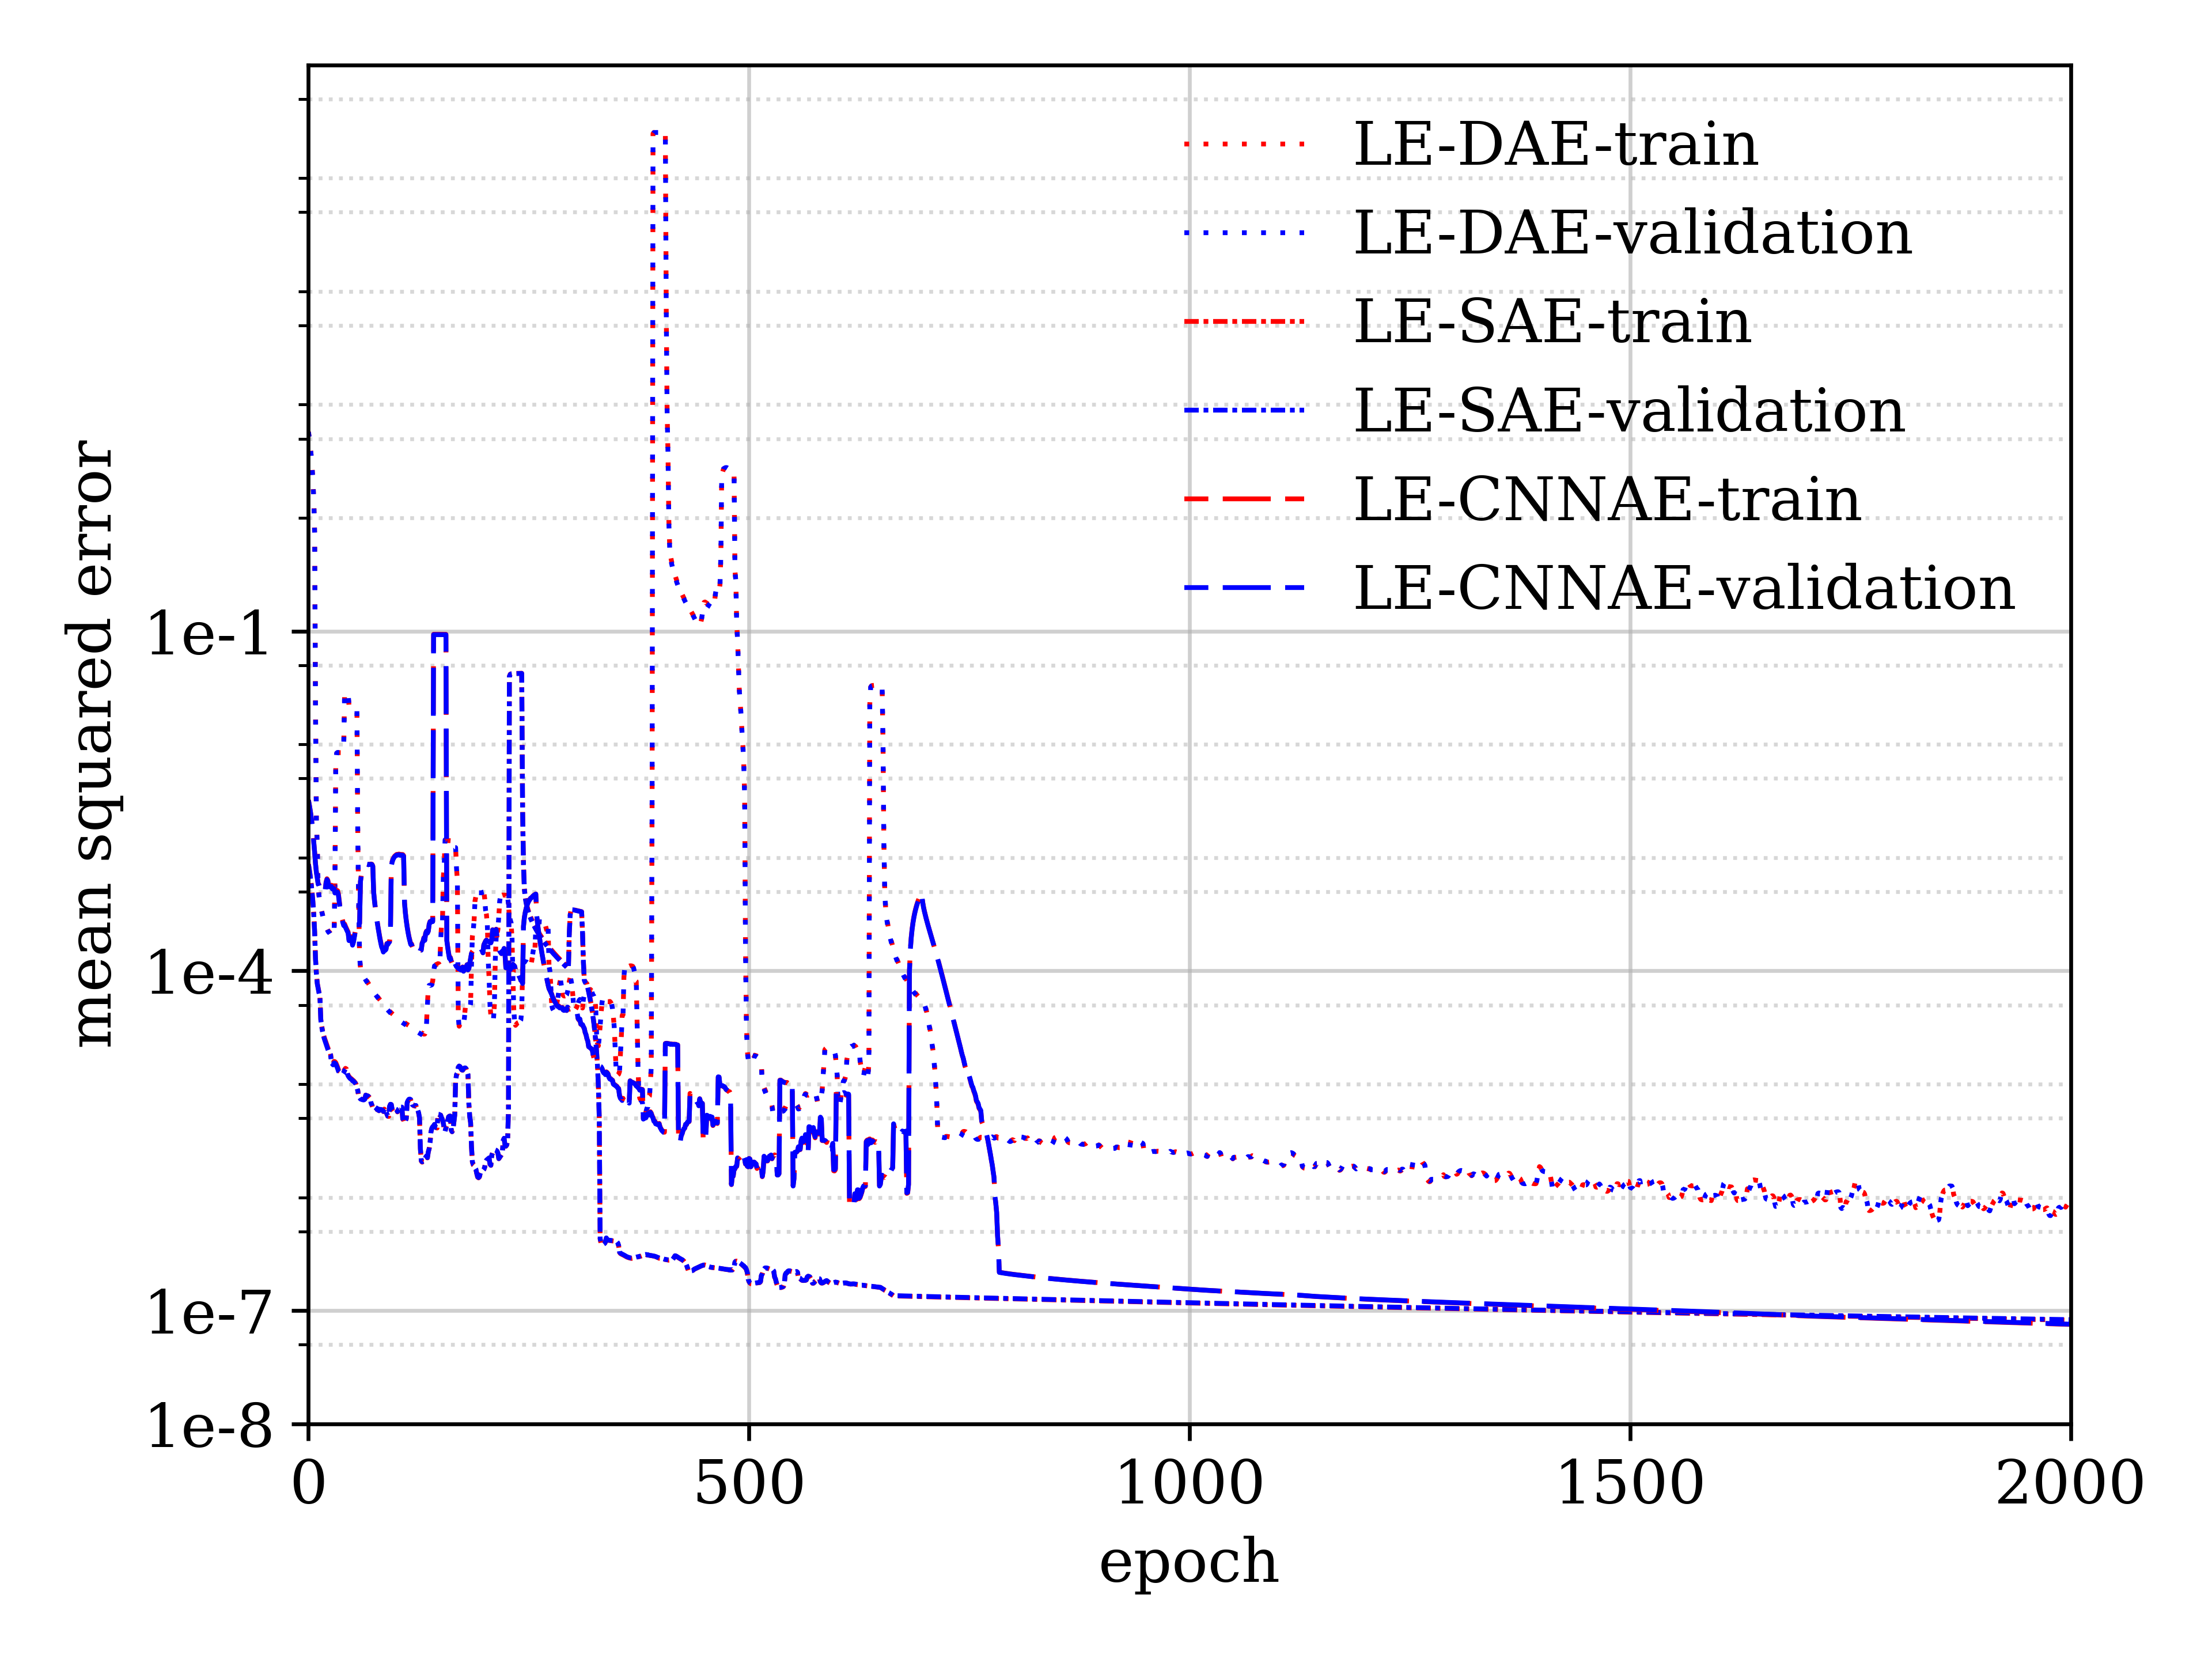
\includegraphics[width=\textwidth]{LE_train_test_history_autoencoder.png}
            \end{center}
            \caption{}
        \end{subfigure}
        \begin{subfigure}[b]{0.49\textwidth}
           \begin{center}
            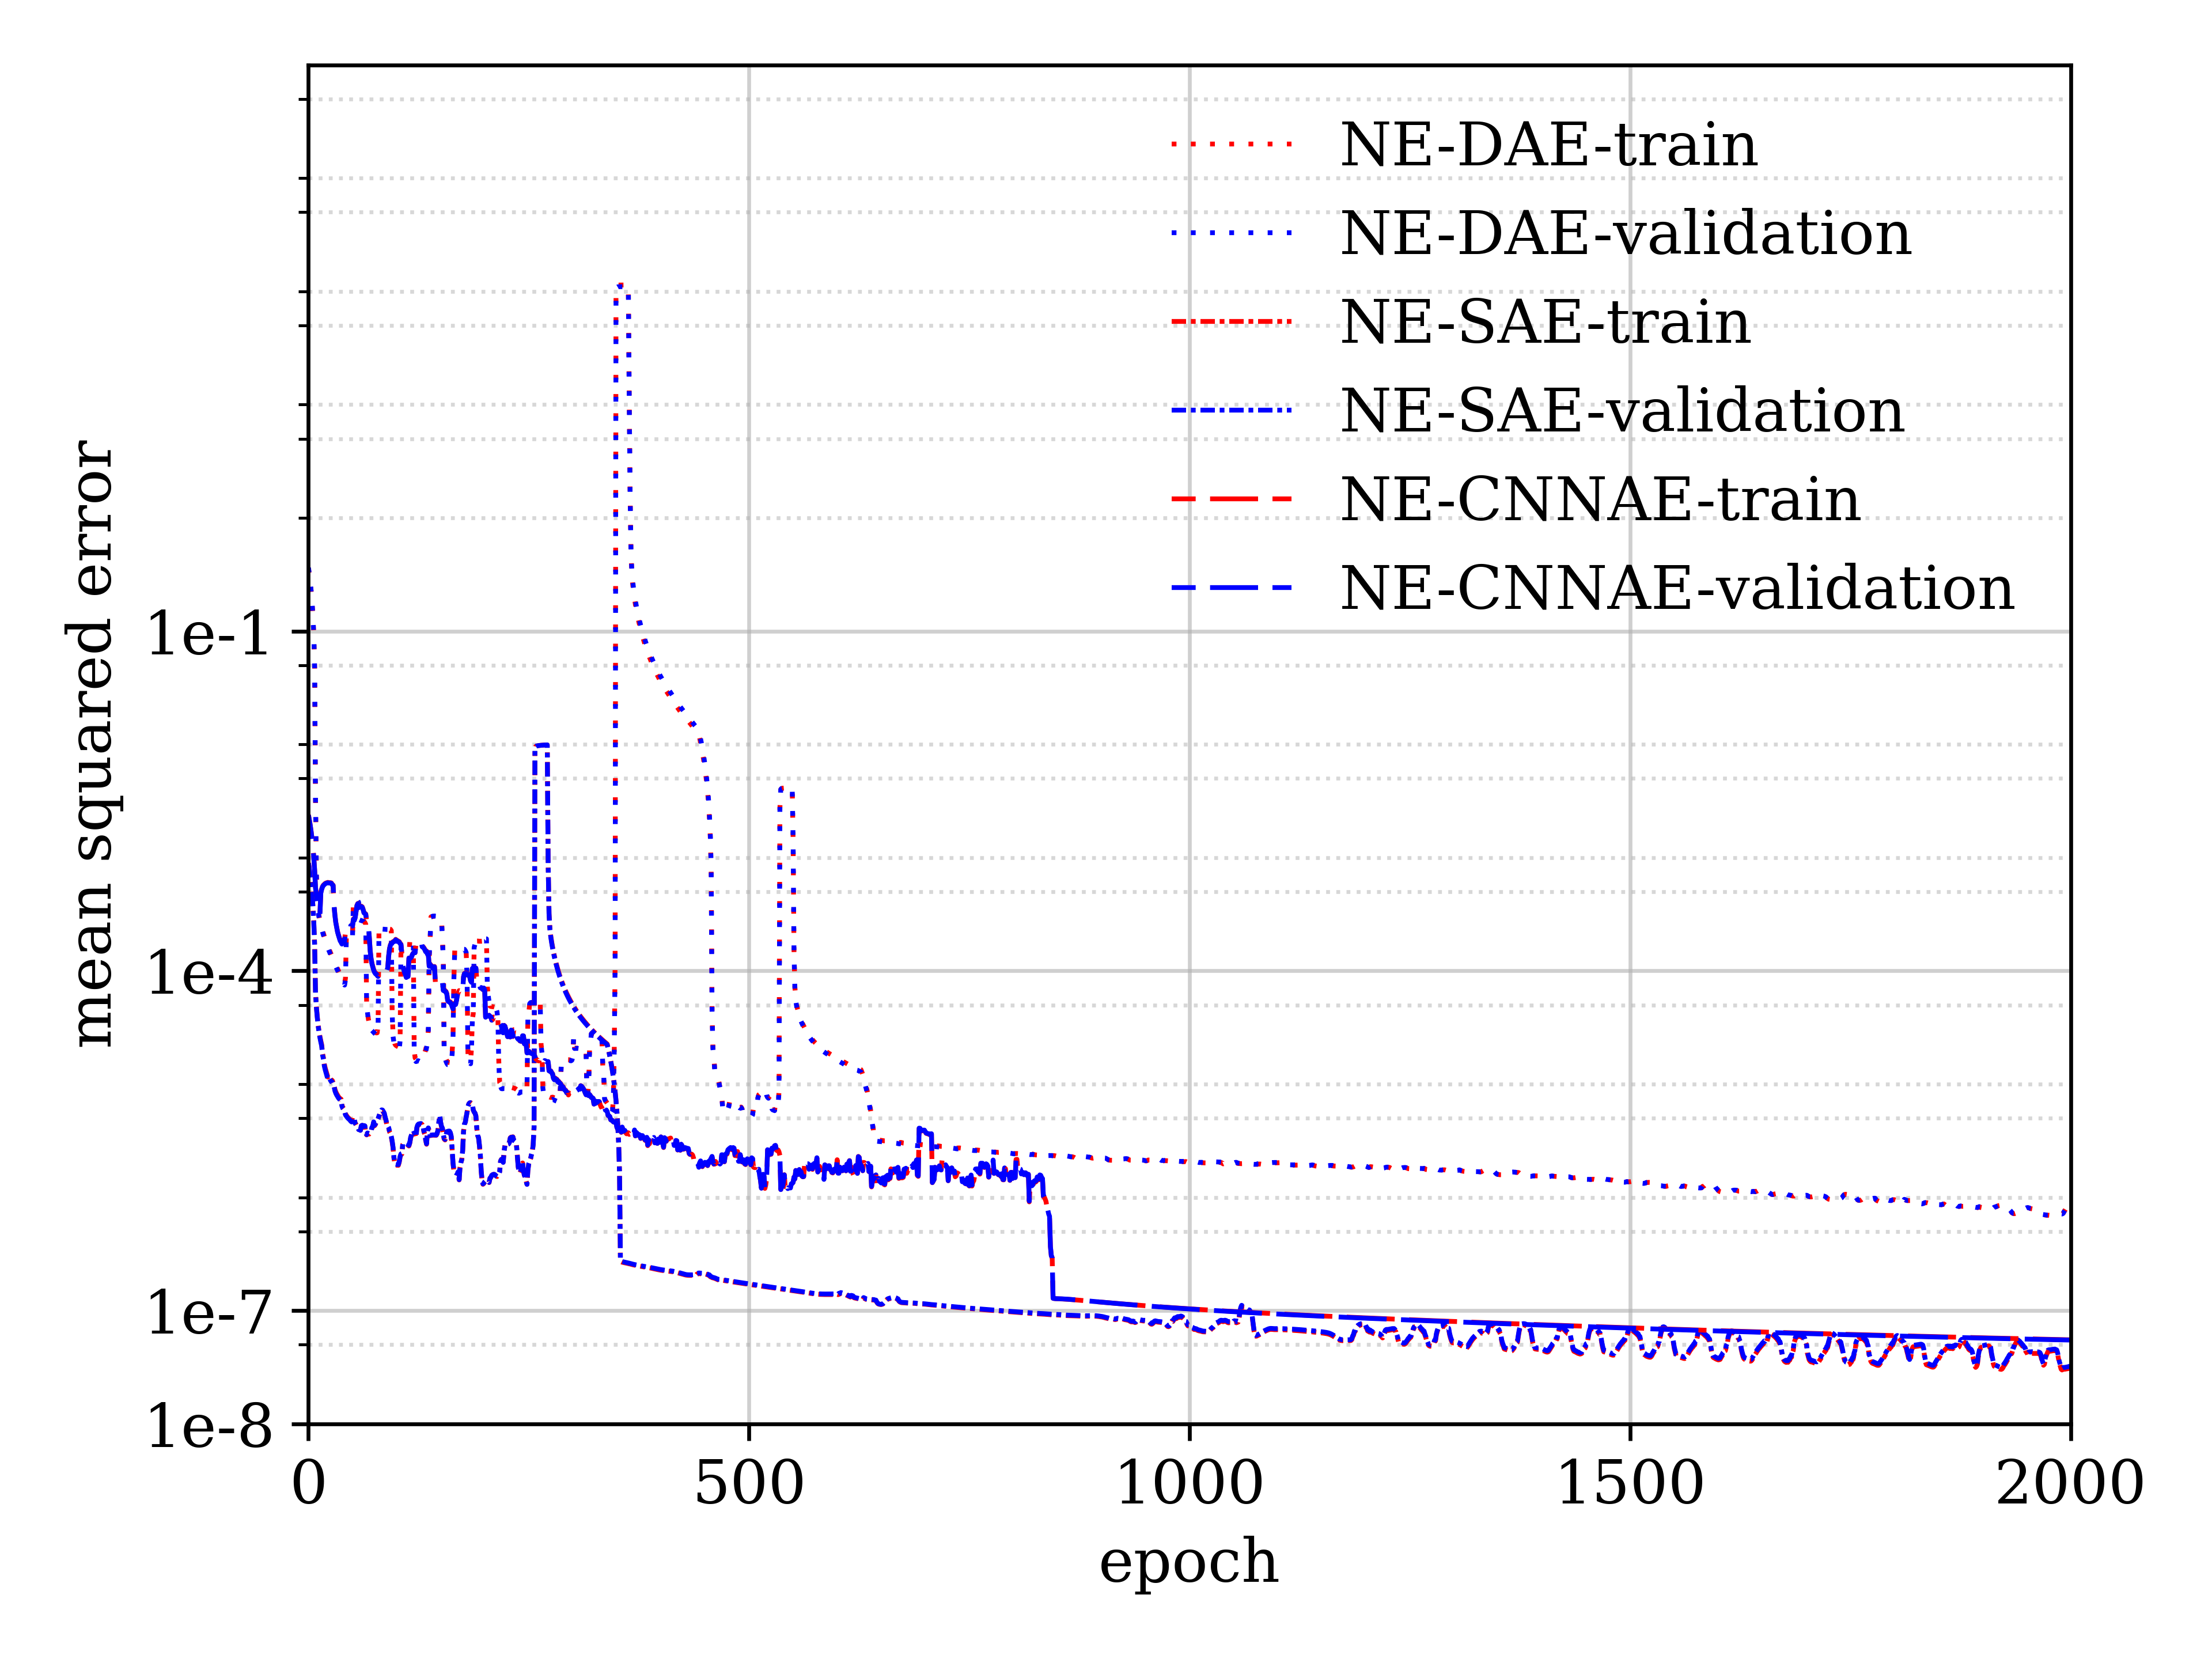
\includegraphics[width=\textwidth]{NE_train_test_history_autoencoder.png}
           \end{center}
            \caption{}
        \end{subfigure}
     \end{center}
        \caption[Loss history ($r = 20$) for the autoencoders.]{Loss (training and validation) history ($r = 20$) for the deep autoencoder (DAE), the sparse autoencoder (SAE), and the proposed convolutional autoencoder (CNNAE) with linear (a) and nonlinear encoder (b). Savitzky-Golay filter is applied to the loss history for better visualization, with filter window length equals to 15, the order of the polynomial used to fit the loss is 1, and the extension contains the nearest input value.}
        \label{fig: train test history}
\end{figure}

We consider the \textit{projection errors} of the autoencoders defined as 
\begin{align}
    l^{\text{proj}}_{\text{LAE}}(\btU; \btPhi) = \frac{\sqrt{\sum_{l=1}^{N_{ic}}\sum_{m=0}^{N_t}\norm{\btu^{\left<m\right>}(u_0^{(\ell)}) - \bar{\btu} - \sum_{i=1}^{r} \inner{\mathbb{R}^N}{\btu^{\left<m\right>}(u_0^{(\ell)}) - \bar{\btu}}{\btphi_i}\btphi_i}^2}}{\sqrt{\sum_{l=1}^{N_{ic}}\sum_{m=0}^{N_t}\norm{\btu^{\left<m\right>}(u_0^{(\ell)})}^2}}
\end{align}
and
\begin{align}
    l^{\text{proj}}_{\text{NAE}}(\btU; \boldsymbol{\Theta}_e, \boldsymbol{\Theta}_d) = \frac{\sqrt{\sum_{l=1}^{N_{ic}}\sum_{m=0}^{N_t}\norm{\btu^{\left<m\right>}(u_0^{(\ell)}) - \bar{\btu} - D(E(\btu^{\left<m\right>}(u_0^{(\ell)}) - \bar{\btu}; \boldsymbol{\Theta}_e); \boldsymbol{\Theta}_d)}^2}}{\sqrt{\sum_{l=1}^{N_{ic}}\sum_{m=0}^{N_t}\norm{\btu^{\left<m\right>}(u_0^{(\ell)})}^2}}\,,
\end{align}
for the linear and nonlinear autoencoders, respectively. The projection error for all autoencoders on the test dataset ($\mu = 1.0$) over different latent space dimensions $r \in \{5, 10, 15, 20\}$ is summarized in Fig.~\ref{fig: proj err burger}.
\begin{figure}[!htb]
    \begin{center}
        \begin{subfigure}[b]{0.49\textwidth}
           \begin{center}
            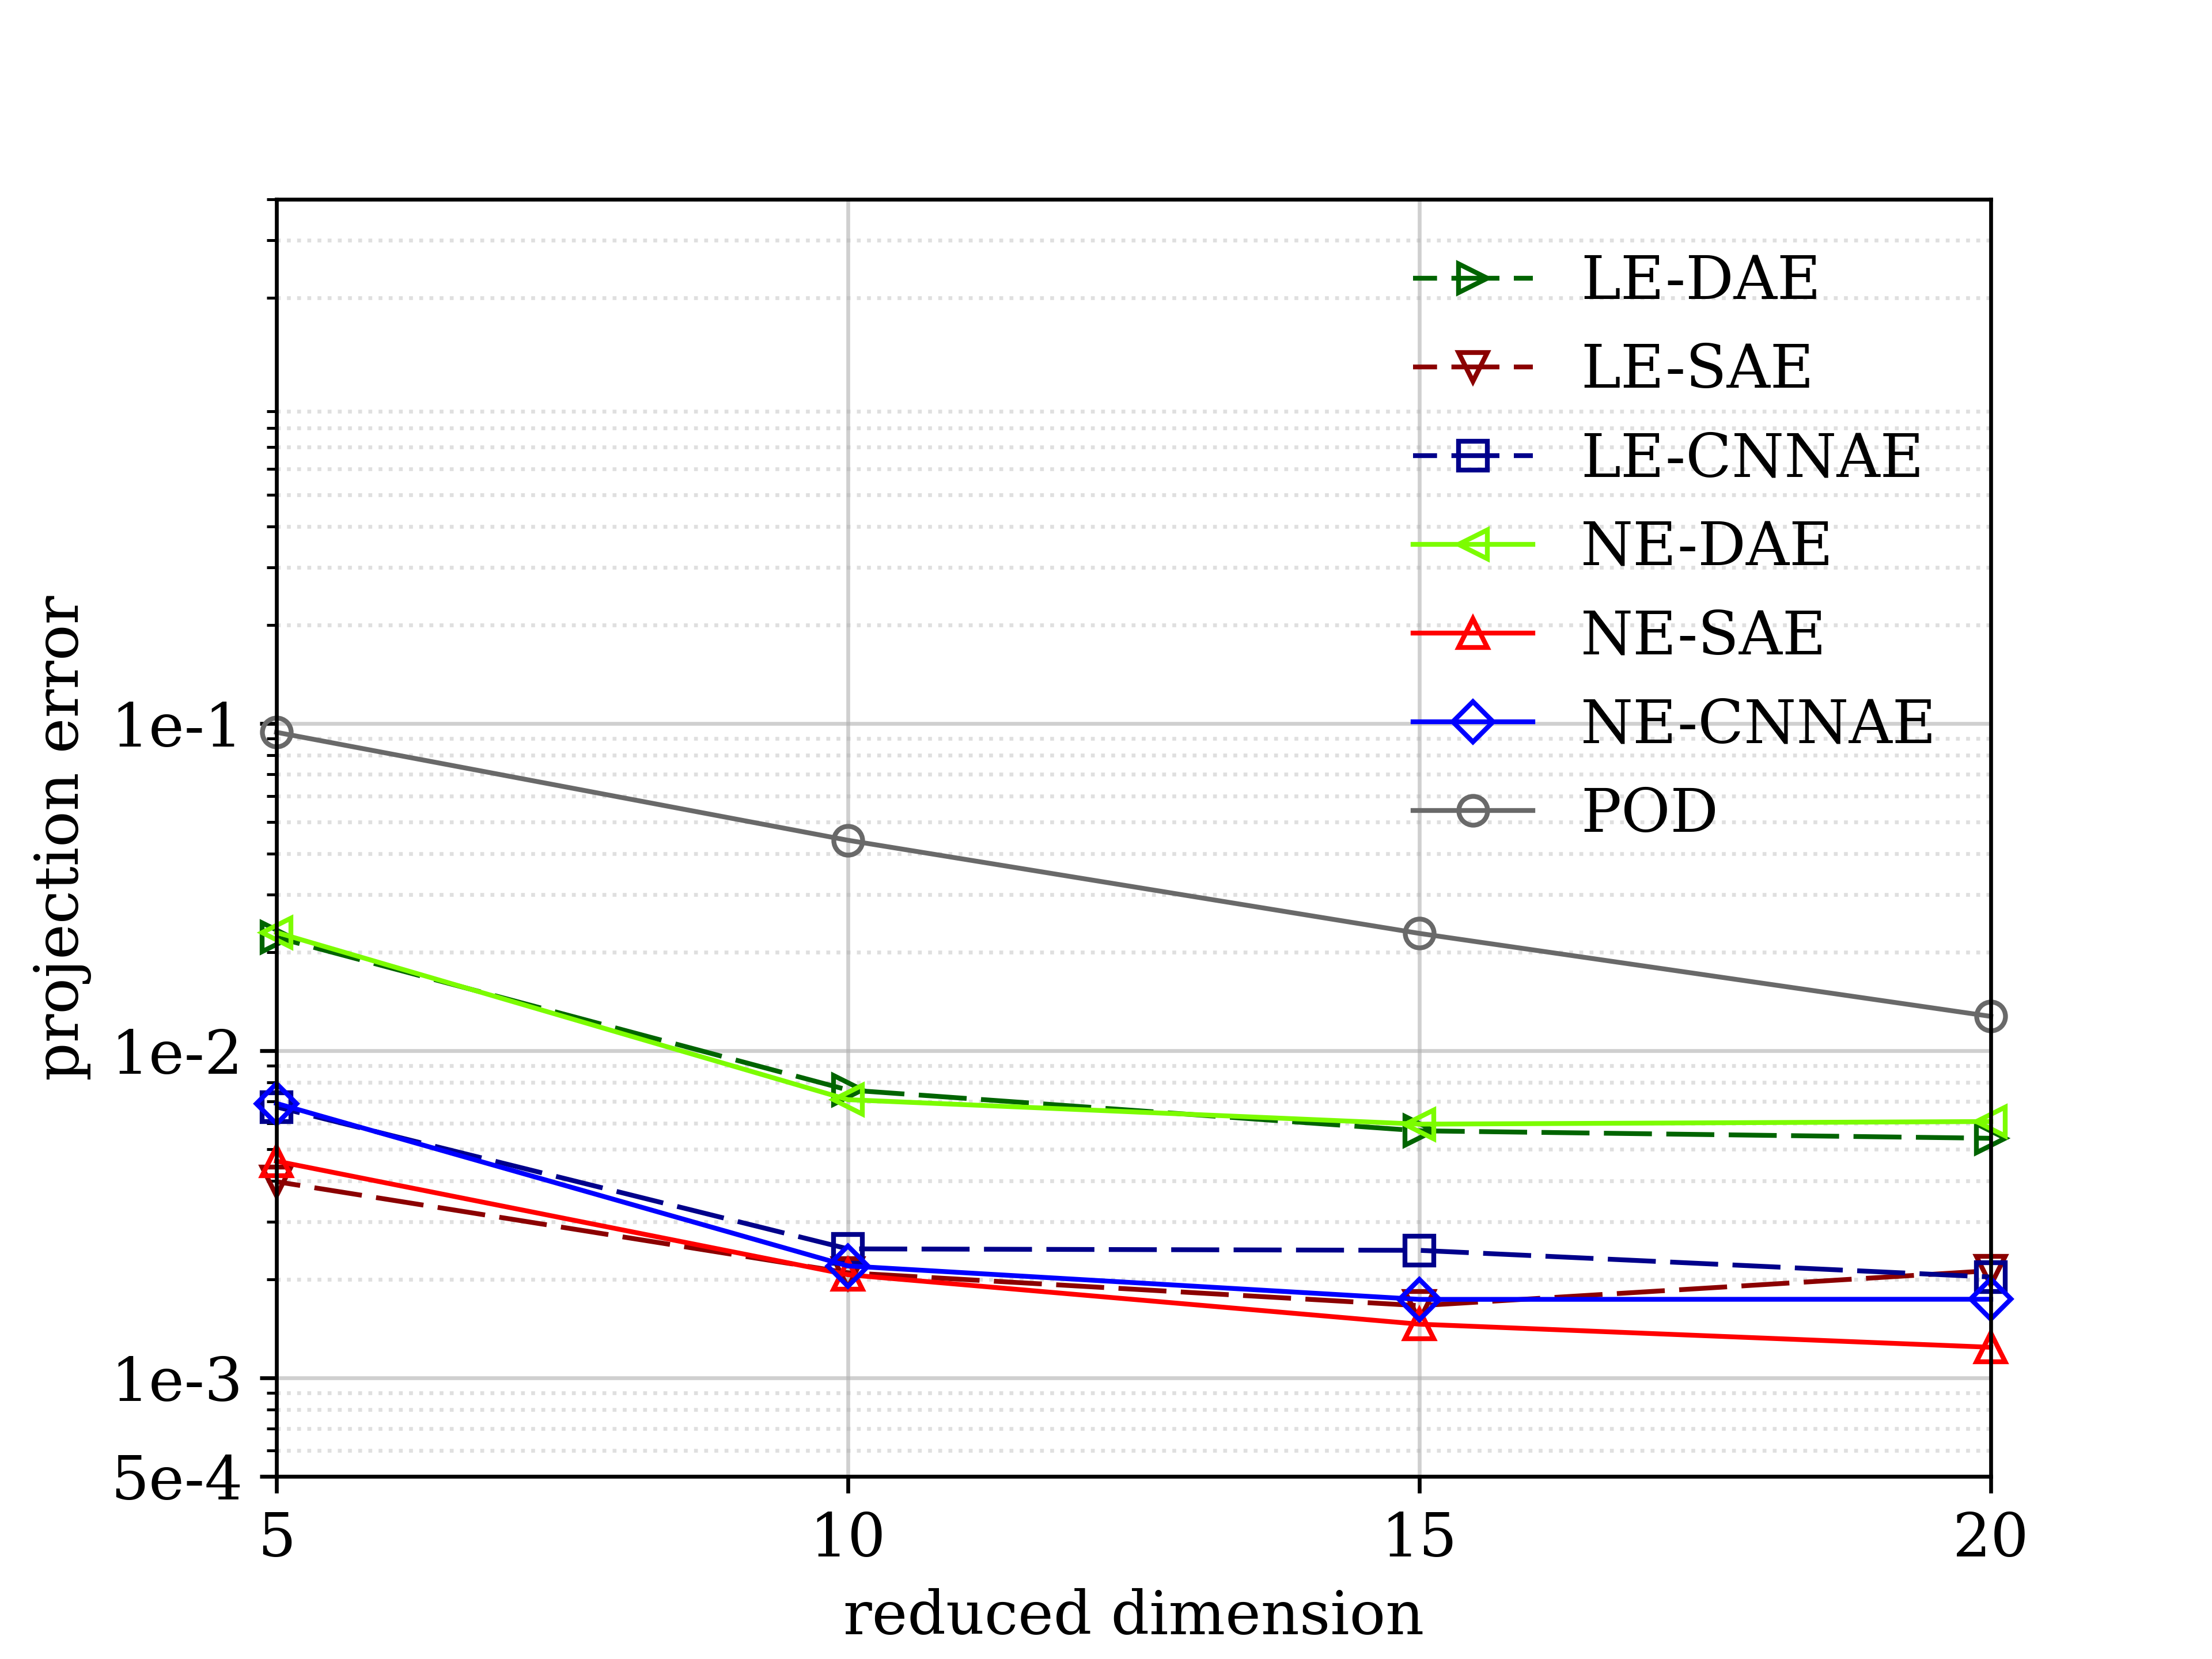
\includegraphics[width=\textwidth]{proj_err_autoencoder_train.png}
           \end{center}
            \caption{}
            \label{fig: proj err burger train}
        \end{subfigure}
        \begin{subfigure}[b]{0.49\textwidth}
            \begin{center}
           \includegraphics[width=\textwidth]{proj_err_autoencoder.png}
            \end{center}
            \caption{}
            \label{fig: proj err burger}
        \end{subfigure}
    \end{center}
        \caption[Projection error and training and test data.]{(a) Projection error over different latent space dimensions on training data with $\mu = \{0.9, 0.95, 1.05, 1.1\}$; (b) Projection error over different latent space dimensions on test data with $\mu = 1.0$.}
\end{figure}

\subsection{Training of Reduced Operators}
We consider two strategies for operator learning between latent spaces. For OPInf, we solve Eq.~\eqref{eq:opinf} for the linear and quadratic reduced operators. For DNNOp, we use 5 hidden layers with sizes of $M_o = 50$, and the swish function as the activation function. The model is trained for 2000 epochs, using the Adam optimizer and an initial learning rate set to $0.01$. We split the training dataset into $n_{\text{batch}} = 100$ batches, and use maximum patience of 100 epochs such that the learning rate will decrease by a factor of 10 when the maximum patience is reached. The reduced operators are trained and paired with the autoencoders given different latent space dimensions, and the training and validation loss (projection error on the rate between latent spaces) histories with r = 20 for all autoencoders paired with the reduced operator are shown in Fig.~\ref{fig: ML op train test history}. Again, it is seen that the training and validation losses exhibit very similar trends and magnitudes, with a good balance between accuracy and overfitting. In Fig.~\ref{fig: operator projection error}, we summarize the projection error of the trained reduced operator given different latent space dimensions. The projection error between latent spaces of the reduced operator is defined as
\begin{align}
    l^{\text{proj}}_{\text{LQ}}(\hat{\btU}; \btA, \btH) = \frac{\sqrt{\sum_{l=1}^{N_{ic}}\sum_{m=0}^{N_t}\norm{\dot{\hat{\btu}}^{\left<m\right>}(u_0^{(\ell)}) - \btA\hat{\btu}^{\left<m\right>} + \btH \left(\hat{\btu}^{\left<m\right>} \otimes \hat{\btu}^{\left<m\right>}\right); \boldsymbol{\Theta}_o)}^2}}{\sqrt{\sum_{l=1}^{N_{ic}}\sum_{m=0}^{N_t}\norm{\dot{\hat{\btu}}^{\left<m\right>}(u_0^{(\ell)})}^2}}\,,
\end{align}
and
\begin{align}
    l^{\text{proj}}_{\text{DNNOp}}(\hat{\btU}; \boldsymbol{\Theta}_o) = \frac{\sqrt{\sum_{l=1}^{N_{ic}}\sum_{m=0}^{N_t}\norm{\dot{\hat{\btu}}^{\left<m\right>}(u_0^{(\ell)}) - \rtO(\hat{\btu}^{\left<m\right>}(u_0^{(\ell)}); \boldsymbol{\Theta}_o)}^2}}{\sqrt{\sum_{l=1}^{N_{ic}}\sum_{m=0}^{N_t}\norm{\dot{\hat{\btu}}^{\left<m\right>}(u_0^{(\ell)})}^2}}\,,
\end{align}
for the quadratic operator inference and DNN-based operator, respectively.

\begin{figure}[!htb]
     \begin{center}
        \begin{subfigure}[b]{0.49\textwidth}
            \begin{center}
            \includegraphics[width=\textwidth]{LE_train_test_history_op.png}
            \end{center}
            \caption{}
        \end{subfigure}
        \begin{subfigure}[b]{0.49\textwidth}
           \begin{center}
            \includegraphics[width=\textwidth]{NE_train_test_history_op.png}
           \end{center}
            \caption{}
        \end{subfigure}
     \end{center}
        \caption[Loss history ($r = 20$) of DNNOp paired with autoencoders.]{Loss (training and validation) history ($r = 20$) of DNNOp paired with linear (a) and nonlinear encoders (b) as well as POD (a). Savitzky-Golay filter is applied to the loss history for better visualization, with filter window length equals to 15, the order of the polynomial used to fit the loss is 1, and the extension contains the nearest input value.}
        \label{fig: ML op train test history}
\end{figure}

\begin{figure}[!htb]
     \begin{center}
        \begin{subfigure}[b]{0.49\textwidth}
            \begin{center}
            \includegraphics[width=\textwidth]{proj_err_operator_train_opinf.png}
            \end{center}
            \caption{}
        \end{subfigure}
        \begin{subfigure}[b]{0.49\textwidth}
            \begin{center}
           \includegraphics[width=\textwidth]{proj_err_operator_train_dnnop.png}
            \end{center}
            \caption{}
        \end{subfigure}
     \end{center}
        \caption[Projection error of the trained reduced operators.]{Projection error of the trained reduced operator $F$ in the latent spaces for (a) quadratic operator inference; and (b) DNN-based operator on the training dataset with $\mu = \{0.9, 0.95, 1.01, 1.1\}$.}
        \label{fig: operator projection error}
\end{figure}

We evaluate the reduced operators' performances between the latent spaces (i.e., the flow map $u_0 \mapsto u(\cdot, t)$, $t > 0$) on the test dataset using the errors given by
\begin{align}
    l^{\text{proj}}_{rom}(\hat{\btU}; \hat{\btu}_0, \boldsymbol{\Theta}_o) = \frac{\sqrt{\sum_{l=1}^{N_{ic}}\sum_{m=0}^{N_t}\norm{\hat{\btu}^{\left<m\right>}(u_0^{(\ell)}) - \hat{\btu}^{\left<m\right>}_{rom}(u_0^{(\ell)})}^2}}{\sqrt{\sum_{l=1}^{N_{ic}}\sum_{m=0}^{N_t}\norm{\hat{\btu}^{\left<m\right>}(u_0^{(\ell)})}^2}}\,,
\end{align}
where $\hat{\btu}^{\left<m\right>}_{rom}(u_0^{(\ell)}) = \mathcal{H}(\hat{\btu}_0(u_0^{(\ell)}); \boldsymbol{\Theta}_o, t_m)$ is the approximated latent solution at a given time step $m$. We solve the reduced order model using the Newton-Raphson method. We evaluate the reduced-order model solution obtained by combining the surrogate operator $\mathcal{H}$ with any of the autoencoders with a projection error in the original high dimensional space, using the error defined as
\begin{align}
    l^{\text{proj}}_{\text{sol}}(\btU; \btPhi, \mathcal{H}(\boldsymbol{\Theta}_o)) = \frac{\sqrt{\sum_{l=1}^{N_{ic}}\sum_{m=0}^{N_t}\norm{\btu^{\left<m\right>}(u_0^{(\ell)}) - \bar{\btu} - \sum_{i=1}^{r} \mathcal{H}(\hat{\btu}_0(u_0^{(\ell)}); \boldsymbol{\Theta}_o, t^m)\btphi_i}^2}}{\sqrt{\sum_{l=1}^{N_{ic}}\sum_{m=0}^{N_t}\norm{\btu^{\left<m\right>}(u_0^{(\ell)})}^2}}
\end{align}
and
\begin{align}
    l^{\text{proj}}_{\text{sol}}(\btU; \boldsymbol{\Theta}_e, \boldsymbol{\Theta}_d, \mathcal{H}(\boldsymbol{\Theta}_o)) = \frac{\sqrt{\sum_{l=1}^{N_{ic}}\sum_{m=0}^{N_t}\norm{\btu^{\left<m\right>}(u_0^{(\ell)}) - \bar{\btu} - D(\mathcal{H}(\hat{\btu}_0(u_0^{(\ell)}); \boldsymbol{\Theta}_o, t^m); \boldsymbol{\Theta}_d)}^2}}{\sqrt{\sum_{l=1}^{N_{ic}}\sum_{m=0}^{N_t}\norm{\btu^{\left<m\right>}(u_0^{(\ell)})}^2}}\,,
\end{align}
for the linear and nonlinear autoencoders, respectively, with $\hat{\btu}_0(u_0^{(\ell)}) = E(\btu_0(u_0^{(\ell)}); \boldsymbol{\Theta}_e)$.

In Fig.~\ref{fig: proj err rom solution}, we show the projection error for the reduced-order model solution over all latent dimensions with different pairs of autoencoders and operators. Note that quadratic operator inference fails to solve this 2D Burger's problem with an error blowing up for $m > 200$ approximately.
\begin{figure}[!htb]
     \begin{center}
        \begin{subfigure}[b]{0.49\textwidth}
            \begin{center}
            \includegraphics[width=\textwidth]{proj_err_xhat_validation.png}
            \end{center}
            \caption{}
        \end{subfigure}
        \begin{subfigure}[b]{0.49\textwidth}
            \begin{center}
           \includegraphics[width=\textwidth]{proj_err_rom_validation.png}
            \end{center}
            \caption{}
        \end{subfigure}
     \end{center}
        \caption[Projection errors on the test data.]{(a) Projection error between the latent spaces obtained from the surrogate operator $\mathcal{H}$; and (b) projection error of the reduced order model solution on the test dataset with $\mu = 1.0$ over different latent space dimension.}
        \label{fig: proj err rom solution}
\end{figure}
The projection error of the reduced-order model for the nonlinear autoencoders is lower than for the linear autoencoders. We summarized ROM solution and their absolute errors of the POD method in Fig.~\ref{fig: pod-burger} for four latent space dimensions. 

\begin{figure}[!htb]
     \begin{center}
        \begin{subfigure}[b]{0.23\textwidth}
            \begin{center}
                \includegraphics[trim = {0, 0, 3cm, 0}, clip, width=\textwidth]{X-rom-POD-5.png}
            \end{center}
            \caption{Solution $r = 5$}
        \end{subfigure}
   \begin{subfigure}[b]{0.23\textwidth}
            \begin{center}
       \includegraphics[trim = {0, 0, 3cm, 0}, clip, width=\textwidth]{X-rom-POD-10.png}
            \end{center}
            \caption{Solution $r = 10$}
        \end{subfigure}
   \begin{subfigure}[b]{0.23\textwidth}
            \begin{center}
       \includegraphics[trim = {0, 0, 3cm, 0}, clip, width=\textwidth]{X-rom-POD-15.png}
            \end{center}
            \caption{Solution $r = 15$}
        \end{subfigure}
   \begin{subfigure}[b]{0.23\textwidth}
       \begin{center}
        \includegraphics[trim = {0, 0, 3cm, 0}, clip, width=\textwidth]{X-rom-POD-20.png}
       \end{center}
       \caption{Solution $r = 20$}
        \end{subfigure}\\  
        \begin{subfigure}[b]{0.23\textwidth}
            \begin{center}
                \includegraphics[trim = {0, 0, 3cm, 0}, clip, width=\textwidth]{X-rom-POD-5-abs-err.png}
            \end{center}
            \caption{Absolute error $r = 5$}
        \end{subfigure}  
        \begin{subfigure}[b]{0.23\textwidth}
            \begin{center}
                \includegraphics[trim = {0, 0, 3cm, 0}, clip, width=\textwidth]{X-rom-POD-10-abs-err.png}
            \end{center}
            \caption{Absolute error $r = 10$}
        \end{subfigure}   
        \begin{subfigure}[b]{0.23\textwidth}
            \begin{center}
                \includegraphics[trim = {0, 0, 3cm, 0}, clip, width=\textwidth]{X-rom-POD-15-abs-err.png}
            \end{center}
            \caption{Absolute error $r = 15$}
        \end{subfigure}    
        \begin{subfigure}[b]{0.23\textwidth}
            \begin{center}
                \includegraphics[trim = {0, 0, 3cm, 0}, clip, width=\textwidth]{X-rom-POD-20-abs-err.png}
            \end{center}
            \caption{Absolute error $r = 20$}
        \end{subfigure}
     \end{center}
     \caption[Solutions and pointwise errors for POD-DNNOp.]{Solutions (a, b, c, d) and pointwise errors (e, f, g, h) for POD-DNNOp with different latent space dimensions.}
        \label{fig: pod-burger}
\end{figure}
Both NE-SAE and NE-CNNAE have a projection error around $2\times10^{-3}$ and deliver the most accurate predictions. Their ROM solutions and associated absolute errors are shown in Fig.~\ref{fig: nesae-burger} and Fig.~\ref{fig: necnnae-burger}. 

\begin{figure}[!htb]
     \begin{center}
        \begin{subfigure}[b]{0.23\textwidth}
          \begin{center}
            \includegraphics[trim = {0, 0, 3cm, 0}, clip, width=\textwidth]{X-rom-NE-SAE-5.png}
          \end{center}
            \caption{Solution $r = 5$}
        \end{subfigure}
   \begin{subfigure}[b]{0.23\textwidth}
       \begin{center}
        \includegraphics[trim = {0, 0, 3cm, 0}, clip, width=\textwidth]{X-rom-NE-SAE-10.png}
       \end{center}
            \caption{Solution $r = 10$}
        \end{subfigure}
   \begin{subfigure}[b]{0.23\textwidth}
            \begin{center}
                \includegraphics[trim = {0, 0, 3cm, 0}, clip, width=\textwidth]{X-rom-NE-SAE-15.png}
            \end{center}
            \caption{Solution $r = 15$}
        \end{subfigure}
   \begin{subfigure}[b]{0.23\textwidth}
            \begin{center}
                \includegraphics[trim = {0, 0, 3cm, 0}, clip, width=\textwidth]{X-rom-NE-SAE-20.png}
            \end{center}
            \caption{Solution $r = 20$}
        \end{subfigure}\\  
        \begin{subfigure}[b]{0.23\textwidth}
            \begin{center}
                \includegraphics[trim = {0, 0, 3cm, 0}, clip, width=\textwidth]{X-rom-NE-SAE-5-abs-err.png}
            \end{center}
            \caption{Absolute error $r = 5$}
        \end{subfigure}  
        \begin{subfigure}[b]{0.23\textwidth}
            \begin{center}
                \includegraphics[trim = {0, 0, 3cm, 0}, clip, width=\textwidth]{X-rom-NE-SAE-10-abs-err.png}
            \end{center}
            \caption{Absolute error $r = 10$}
        \end{subfigure}   
        \begin{subfigure}[b]{0.23\textwidth}
            \begin{center}
                \includegraphics[trim = {0, 0, 3cm, 0}, clip, width=\textwidth]{X-rom-NE-SAE-15-abs-err.png}
            \end{center}
            \caption{Absolute error $r = 15$}
        \end{subfigure}    
        \begin{subfigure}[b]{0.23\textwidth}
            \begin{center}
                \includegraphics[trim = {0, 0, 3cm, 0}, clip, width=\textwidth]{X-rom-NE-SAE-20-abs-err.png}
            \end{center}
            \caption{Absolute error $r = 20$}
        \end{subfigure}
     \end{center}
     \caption[Solutions and pointwise errors for NE-SAE-DNNOp.]{Solutions (a, b, c, d) and pointwise errors (e, f, g, h) for NE-SAE-DNNOp with different latent space dimensions.}
        \label{fig: nesae-burger}
\end{figure}

\begin{figure}[!htb]
     \begin{center}
        \begin{subfigure}[b]{0.23\textwidth}
            \begin{center}
                \includegraphics[trim = {0, 0, 3cm, 0}, clip, width=\textwidth]{X-rom-NE-CNNAE-5.png}
            \end{center}
            \caption{Solution $r = 5$}
        \end{subfigure}
   \begin{subfigure}[b]{0.23\textwidth}
            \begin{center}
                \includegraphics[trim = {0, 0, 3cm, 0}, clip, width=\textwidth]{X-rom-NE-CNNAE-10.png}
            \end{center}
            \caption{Solution $r = 10$}
        \end{subfigure}
   \begin{subfigure}[b]{0.23\textwidth}
            \begin{center}
                \includegraphics[trim = {0, 0, 3cm, 0}, clip, width=\textwidth]{X-rom-NE-CNNAE-15.png}
            \end{center}
            \caption{Solution $r = 15$}
        \end{subfigure}
   \begin{subfigure}[b]{0.23\textwidth}
           \begin{center}
            \includegraphics[trim = {0, 0, 3cm, 0}, clip, width=\textwidth]{X-rom-NE-CNNAE-20.png}
           \end{center}
            \caption{Solution $r = 20$}
        \end{subfigure}\\  
        \begin{subfigure}[b]{0.23\textwidth}
            \begin{center}
                \includegraphics[trim = {0, 0, 3cm, 0}, clip, width=\textwidth]{X-rom-NE-CNNAE-5-abs-err.png}
            \end{center}
            \caption{Absolute error $r = 5$}
        \end{subfigure}  
        \begin{subfigure}[b]{0.23\textwidth}
            \begin{center}
                \includegraphics[trim = {0, 0, 3cm, 0}, clip, width=\textwidth]{X-rom-NE-CNNAE-10-abs-err.png}
            \end{center}
            \caption{Absolute error $r = 10$}
        \end{subfigure}   
        \begin{subfigure}[b]{0.23\textwidth}
            \begin{center}
                \includegraphics[trim = {0, 0, 3cm, 0}, clip, width=\textwidth]{X-rom-NE-CNNAE-15-abs-err.png}
            \end{center}
            \caption{Absolute error $r = 15$}
        \end{subfigure}    
        \begin{subfigure}[b]{0.23\textwidth}
            \begin{center}
                \includegraphics[trim = {0, 0, 3cm, 0}, clip, width=\textwidth]{X-rom-NE-CNNAE-20-abs-err.png}
            \end{center}
            \caption{Absolute error $r = 20$}
        \end{subfigure}
     \end{center}
     \caption[Solutions and pointwise errors for NE-CNNAE-DNNOp.]{Solutions (a, b, c, d) and pointwise errors (e, f, g, h) for NE-CNNAE-DNNOp with different latent space dimensions.}
        \label{fig: necnnae-burger}
\end{figure}

The absolute errors decrease together when latent dimension increases. However, oscillations in the ROM solution of the POD method can still be observed for $r = 20$. These oscillations can also be observed from the ROM solution with the LE-DAE and NE-DAE, but are not present for NE-CNNAE and NE-SAE when $r \in \{15, 20\}$.

The adaptivity in the bases promoted in the CNNAE approach is illustrated in Fig.~\ref{fig:adaptivity}, which shows how one particular basis (here, $D_4$) evolves as a function of time (similar responses are obtained for the other bases).
\begin{figure}[!htb]
     \begin{center}
        \begin{subfigure}[b]{0.22\textwidth}
            \begin{center}
                \includegraphics[trim = {0, 0, 3cm, 0}, clip, width=\textwidth]{Figure_Base_3_Snapshot_2.pdf}
            \end{center}
            \caption{$M = 201$}
        \end{subfigure}
   \begin{subfigure}[b]{0.22\textwidth}
       \begin{center}
        \includegraphics[trim = {0, 0, 3cm, 0}, clip, width=\textwidth]{Figure_Base_3_Snapshot_6.pdf}
       \end{center}
            \caption{$M = 601$}
        \end{subfigure}
   \begin{subfigure}[b]{0.22\textwidth}
       \begin{center}
        \includegraphics[trim = {0, 0, 3cm, 0}, clip, width=\textwidth]{Figure_Base_3_Snapshot_10.pdf}
       \end{center}
            \caption{$M = 1001$}
        \end{subfigure}
   \begin{subfigure}[b]{0.26\textwidth}
       \begin{center}
        \includegraphics[trim = {0, 0, 0cm, 0}, clip, width=\textwidth]{Figure_Base_3_Snapshot_14.pdf}
       \end{center}
            \caption{$M = 1401$}
        \end{subfigure}
     \end{center}
\caption[Evolution of the fourth basis in CNNAE.]{This figure illustrates adaptivity by showing the evolution of the fourth basis in Eq.~\eqref{eq: cnn decoder}. Here, we take the basis at the 101st time step as reference, and plot the evolution of the difference $\Delta D_4(M) = D_4(\hat{u}_4^{\left<M\right>}; \hat{\btu}^{\left<M\right>}) - D_4(\hat{u}_4^{\left<101\right>}; \hat{\btu}^{\left<101\right>})$ at selected time steps (namely, 201, 601, 1001, and 1401). Note that the basis is shown in physical space to enable proper visualization.}
\label{fig:adaptivity}
\end{figure}
This adaptivity mechanism helps capture the features exhibited by the solution as the simulation progresses, hence facilitating interpretation.

The performance of vectorized implicit time integration was assessed by measuring the  computational cost of flow map estimation for 1500 time steps, using wall-clock time and multiple GPUs --- as speed up also varies based on the hardware itself. The timing is obtained by performing calculations on NVIDIA RTX A4500 (64 bits, 33MHz, 20 GB), and NVIDIA RTX A6000 (64 bits, 33MHz, 48 GB), NVIDIA GeForce 4080 (64 bits, 33MHz, 16 GB). The wall-clock times are provided in Tab.~\ref{Tab:A4500}. The algorithm improves performance for $r \geq 15$, regardless of chunk size, with a maximum speed-up of 25.48 when solving the reduced order model in the latent space (as compared to serial solving for the ROM). Observe that $r \geq 15$, speed-ups do not decrease as the chunk size reaches 100. This implies that memory limitation (hardware limitation) was not reached for any of the GPUs, which indicates that the tested chunk sizes may be suboptimal. For $r = 10$ and a chunk size equal to 100, speed-ups decrease for all configurations, which suggests that for this specific case, the required number of nonlinear iterations is larger than for the other cases. For this choice of parameters, the solver eventually fails, hence resulting in infinite projection errors (as shown in Tab.~\ref{Tab:A4500}). To further support this explanation, the maximum number of Newton-Raphson (N-R) iterations required for each chunk when solving the adjoint integration problems is also reported. It is seen that when $r = 10$ and for a chunk size equal to 100, the number of nonlinear iterations reaches its maximum allowed value (set to 100), for all GPUs. This behavior is a manifestation of the interplay between the chunk size, the initial guess in the Newton-Raphson solver, and the latent space dimension. When the dimension $r$ are large enough, the solution can be obtained even under poor initialization: the number of solver iterations then increases together with the chunk size. This can be seen in Tab.~\ref{Tab:A4500}: when the chunk size equals 1, around 2 iterations are necessary to reach convergence, while around 10 iterations are needed for a chunk size set to 100.
\begin{table}[!ht]
    \caption[Wall-clock times on multiple GPUs.]{Wall-clock times at different latent space dimensions and chunk size on NVIDIA RTX A4500, NVIDIA RTX A6000, and NVIDIA GeForce 4080 for 1500 time steps on the test dataset ($\mu = 1.0$). The shortest wall-clock time is obtained when $r = 15$ using NVIDIA RTX A6000 with 1.32 seconds.}
    \label{Tab:A4500}
    \begin{center}
        \small
    \begin{tabular}{|c|c|c|c|c|c|c|c|c|c|c|c|c|}
    \hline
    \multicolumn{13}{|c|}{NVIDIA RTX A4500} \\ \cline{1-13}
    Reduced dimension $r$ & \multicolumn{4}{|c|}{10} & \multicolumn{4}{|c|}{15} & \multicolumn{4}{|c|}{20}\\ \hline
    Chunk size & 1 & 10 & 50 & 100 & 1 & 10 & 50 & 100 & 1 & 10 & 50 & 100 \\ \hline
    Projection error (\%) & 0.33 & 0.33 & 0.33 & INF & 0.34 & 0.34 & 0.34 & 0.34 & 0.23 & 0.23 & 0.23 & 0.23 \\ \hline
    N-R iterations $\#$ & 2 & 3 & 6 & 100 & 3 & 3 & 5 & 7 & 3 & 4 & 7 & 12 \\ \hline
    Wall time (sec) & 34.08 & 5.10 & 1.61 & 6.94 & 34.65 & 5.06 & 1.62 & 1.36 & 34.46 & 5.07 & 1.78 & 1.48 \\ \hline 
    Speed-up & 1 & 6.68 & 21.17 & 4.91 & 1 & 6.85 & 21.39 & \textbf{25.48} & 1 & 6.80 & 19.36 & 23.28 \\ \hline
    \multicolumn{13}{|c|}{NVIDIA RTX A6000} \\ \cline{1-13}
    Reduced dimension $r$ &\multicolumn{4}{|c|}{10} & \multicolumn{4}{|c|}{15} & \multicolumn{4}{|c|}{20}\\ \hline
    Chunk size & 1 & 10 & 50 & 100 & 1 & 10 & 50 & 100 & 1 & 10 & 50 & 100 \\ \hline
    Projection error (\%) & 0.33 & 0.33 & 0.33 & INF & 0.34 & 0.34 & 0.34 & 0.34 & 0.23 & 0.23 & 0.23 & 0.23 \\ \hline
    N-R iterations $\#$ & 2 & 3 & 6 & 100 & 3 & 3 & 5 & 6 & 2 & 3 & 6 & 8 \\ \hline 
    Wall time (sec) & 10.49 & 2.4 & 1.2 & 5.87 & 10.72 & 2.34 & 1.42 & \textbf{1.32} & 14.19 & 2.26 & 2.08 & 1.38 \\ \hline 
    Speed-up & 1 & 4.37 & 8.74 & 1.79 & 1 & 4.58 & 7.55 & 8.12 & 1 & 6.59 & 7.16 & 10.80 \\ \hline
    \multicolumn{13}{|c|}{NVIDIA GeForce 4080} \\ \cline{1-13}
    Reduced dimension $r$ & \multicolumn{4}{|c|}{10} & \multicolumn{4}{|c|}{15} & \multicolumn{4}{|c|}{20}\\ \hline
    Chunk size & 1 & 10 & 50 & 100 & 1 & 10 & 50 & 100 & 1 & 10 & 50 & 100 \\ \hline
    Projection error (\%) & 0.33 & 0.33 & 0.33 & INF & 0.34 & 0.34 & 0.34 & 0.34 & 0.23 & 0.23 & 0.23 & 0.23 \\ \hline
    N-R iterations $\#$ & 2 & 3 & 6 & 100 & 3 & 3 & 5 & 7 & 2 & 3 & 5 & 7 \\ \hline 
    Wall-clock time (sec) & 14.74 & 1.37 & 0.73 & 8.69 & 13.02 & 2.59 & 1.50 & 1.51 & 13.52 & 2.62 & 1.64 & 1.64 \\ \hline 
    Speed-up & 1 & 10.76 & 20.19 & 1.67 & 1 & 5.03 & 8.67 & 8.62 & 1 & 5.16 & 8.24 & 8.24 \\ \hline
    \end{tabular}
    \end{center}
 \end{table}

We also evaluated the performance of NE-CNNAE on other datasets beyond the range of the training dataset, for $\mu = 1.11$, $1.12$, $1.13$, $1.14$, $1.15$. The projection errors of the reduced-order model and the projection error between the latent spaces of NE-CNNAE with $n = 20$ are shown in Fig.~\ref{fig: extrapolate}. This figure illustrates how the accuracy decreases in the extrapolation regime, with an increase of almost one order of magnitude between $\mu = 1.1$ (included in the training dataset) and $\mu = 1.15$.

\begin{figure}[!htb]
     \begin{center}
        \includegraphics[width=0.49\textwidth]{extrapolate.png}
     \end{center}
     \caption[Projection error on extrapolated dataset.]{Projection error between the latent spaces obtained from the surrogate operator $\mathcal{H}$ and projection error of the reduced-order model solution on the test dataset with $\mu = 1.11$, $1.12$, $1.13$, $1.14$, $1.15$ when $n = 20$ of NE-CNNAE.}
        \label{fig: extrapolate}
\end{figure}


\subsection{Remarks on Complexity and Time Step Size Dependency}\label{subsec:time-dependency}

For nonlinear autoencoders, the number of trainable parameters can be considered as a measure of model complexity. For the above numerical example, with a latent dimension equal to 20, DAE has around 140 millions of trainable parameters, SAE has around 25 millions of trainable parameters, and the proposed CNNAE (which achieves best performance, together with SAE) has around 1 million trainable parameters. When training the models for 22 batches per epoch on NVIDIA RTX A4500 (64 bits, 33 MHz, 20 GB), with each batch containing approximately 246 time steps of solutions with a latent dimension set to 20, LE-DAE requires 14.70 seconds, LE-SAE 14.96 seconds, LE-CNNAE 1.56 seconds, NE-DAE 14.72 seconds, NE-SAE 14.98 seconds, and NE-CNNAE requires 1.58 seconds per epoch (average wall-clock time over 100 epochs).

It should be noticed that the considered operator learning strategies are, by construction, dependent on the time step size used for the training dataset. To quantify this effect, projection errors (in latent space and for the reduced-order model) obtained with NE-SAE and NE-CNNAE, and refined step sizes, are shown in Fig.~\ref{fig: time step size dependency}. Here, the surrogates were trained with a time step size denoted by $\Delta t$, and the projection errors are evaluated by running both the FOM and ROMs with decreasing time step sizes: $\{\Delta t, \Delta t / 2, \Delta t / 4, \Delta t / 8\}$.
\begin{figure}[!htb]
     \begin{center}
        \begin{subfigure}[b]{0.49\textwidth}
            \begin{center}
                \includegraphics[width=\textwidth]{rom_hat_step_size.png}
            \end{center}
            \caption{}
        \end{subfigure}
        \begin{subfigure}[b]{0.49\textwidth}
            \begin{center}
                \includegraphics[width=\textwidth]{rom_time_step_size.png}
            \end{center}
            \caption{}
        \end{subfigure}
     \end{center}
        \caption[Time step-size dependency.]{(a) Projection error of the solution in the latent space; and (b) projection error of the reduced-order model  with $r = 20$ on the test dataset over different time step sizes. Here, $\Delta t$ is the time step size used for training the autoencoders and the reduced operators.}
        \label{fig: time step size dependency}
\end{figure}
It is seen that both errors substantially increase as the time resolution is refined, which is consistent with results reported elsewhere (see, e.g., \cite{ZHU2018415} for similar behavior with space discretization). The increase in the ROM projection error is larger for CNNAE than for SAE (see the right panel in Fig.~\ref{fig: time step size dependency}), which may be attributed to the fact that the adaptive basis is constructed for a given time step size.
\chapter{Concurrent Multiscale Simulations of Nonlinear Random Materials Using Probabilistic Learning}
\label{chap:fe2}

 In this work, we explore an alternative path to address this problem and seek to construct a statistical surrogate model where the forward map of interest (specifically, the non-local constitutive model) is approximated using statistical conditioning. Instead of calibrating a regression model between the input (e.g., the deformation gradient) and the output (say, a stress measure), we aim to directly generate samples from the input-output joint probability measure, and to estimate quantities of interest through conditional means. This viewpoint requires the use of a generative model capable of accurately capturing measure concentration and the (unknown) geometry of the support of the measure in the small data limit --- a task that remains particularly challenging for strongly non-Gaussian distributions in high dimensions. We note that the construction of generative models is a vibrant topic across many scientific communities, and providing an extensive review on existing techniques is beyond the scope of this paper. In the present study, we employ probabilistic learning on manifolds (PLoM) \cite{Soize2016,Soize2020c,Soize2022a} to perform this task. The choice of this technique is motivated by (\textit{i}) its capability to sample the probability measure defined by the training dataset and in particular, to respect measure concentration and support information (as demonstrated in \cite{Farhat2019,Ghanem2019, Arnst2021,Capiez2022,Ghanem2022, Safta2022, Sinha2023, Zhong2023, Ezvan2023, Almeida2023,Govindjee2023,Soize2024}), (\textit{ii}) relative ease of implementation, and (\textit{iii}) its reliance on low-dimensional, interpretable parameterization. Our main contributions are as follows. First, we formulate the approximation of the non-local homogenized response in nonlinear elasticity as a learning problem. Second, we perform extensive numerical studies and address the validation of the framework under two scenarios relevant to inverse problem solving and forward propagation. In the former case, the approach can be used, for instance, to calibrate hyperparameters in the material model at fine scale, integrating data at the coarse scale. The latter case represents the classical surrogate setting with aleatoric uncertainties induced by subscale randomness (without separation of scales). Notice that while the proposed developments are derived in the context of nonlinear elasticity, they remain applicable to other classes of constitutive models --- at the expense of adapting the mechanistic parameterization.

This section is organized as follows. The multiscale mechanistic framework is first introduced in Section \ref{sec:mechanics}. The deterministic scale-coupling problems (and their stochastic counterparts) are presented, together with the stochastic model enabling the representation of material randomness at mesoscale. Section \ref{sec:PLoM} provides a comprehensive overview on the probabilistic learning framework, including both theoretical and algorithmic aspects. In Section \ref{sec:application}, the proposed framework is applied in the context of finite elasticity. The two aforementioned scenarios are specifically introduced to assess the robustness of the method (in probability law).

\section{Description of the Mechanistic Framework}\label{sec:mechanics}
\subsection{Definition of the Structural Problem}\label{subsec:def-struc-pb}

Let $\Omega_\text{str}$ be an open bounded domain in $\mathbb{R}^d$ (here, $d = 2$ without loss of methodological generality) representing the reference configuration for the structure of interest, and denote by $\partial \Omega_\text{str}$ the boundary of $\Omega_\text{str}$. For any material point $\bfx \in \Omega_\text{str}$, the spatial point $\bfx^\varphi$ in the deformed configuration $\Omega_{\text{str}}^\varphi$ is given by $\bfx^\varphi = \varphi (\bfx)$, where $\varphi$ is the deformation map. To make the presentation concrete, we assume that the material (at fine scale) is hyperelastic, compressible and isotropic. In addition, we consider a Saint Venant–Kirchhoff model, with a strain energy density function given by
\begin{align}
    \psi([E]) = \frac{\lambda}{2} [\textnormal{tr}([E])]^2 + \mu \, \textnormal{tr}([E]^2)\,,\label{eq: strain energy density}
\end{align}
where $\lambda$ and $\mu$ are the Lamé parameters. Note that the proposed approach can accommodate other types of constitutive behaviors, and that the above choice pertaining to the strain energy density function is not expected to impact the methodological results presented in this research. 

For any $\bfx \in \Omega_\text{str}$, the deformation gradient $[F]$ is a second-order tensor defined as $[F] = [\boldsymbol{\nabla}_{\bfx} \bfx^\varphi]$. The right Cauchy-Green deformation tensor is defined as $[C] = [F]^T [F]$, and the Green-Lagrange strain tensor defined as $[E] = \frac{1}{2}([C] - [I])$. In a general setting, the strong form (resulting from the balance of linear momentum) of the boundary value problem (BVP) in the reference configuration is stated as \cite{ciarlet}
\begin{align}
    \boldsymbol{\nabla}_{\bfx} [P(\bfx)] + \bfb(\bfx)  = \mathbf{0}\,,& \quad \forall\,\bfx \in \Omega_\text{str}\,, \label{eq: stress divergence structural}\\
    \bfu(\bfx) = \overline{\bfu}(\bfx)\,,& \quad \forall\, \bfx \in \partial \Omega_\text{str}^D\,,\\
    [P(\bfx)] \cdot \bfn(\bfx) = \overline{\bft}(\bfx)\,,& \quad \forall\, \bfx \in \partial \Omega_\text{str}^N\,,
\end{align}
where $\boldsymbol{\nabla}_{\bfx}$ denotes the divergence operator in the reference configuration, $[P]$ is the first Piola-Kirchhoff stress tensor defined as
\begin{equation}
    [P] = \frac{\partial \psi([F])}{\partial [F]}\,,
\end{equation}
the vector $\bfb$ is the body force, $\bfn$ is unit vector normal to the boundary in the reference configuration, $\overline{\bfu}$ and $\overline{\bft}$ are given smooth vector fields on the Dirichlet and Neumann boundaries, denoted by $\partial \Omega_\text{str}^D$ and $\partial \Omega_\text{str}^N$ respectively. The solution to the above problem is classically sought (in an appropriate function space) as a stationary point of the following energy functional \cite{ciarlet,wriggers2008nonlinear,bonet_wood_2008}:
\begin{align}
    \Pi(\varphi) &= \int_B \psi([F]) \, dV - \int_{B} \bfb \cdot \varphi\,dV - \int_{\partial B_N} \overline{\bft} \cdot \varphi\,dA\,.
\end{align}
In this work, we apply a Dirichlet boundary condition $\overline{\bfu}$ on $\partial \Omega_\text{str}$ (i.e., no traction is applied, and the body force is neglected).

\subsection{Definition of the Macroscopic Problem in the Context of Concurrent Multiscale Approaches}\label{subsec:def-mac-pb}

Let $\Omega_\text{mac} \subset \Omega_\text{str}$ denote the reference configuration for the subdomain where the surrogate must be constructed, and denote by $\partial \Omega_\text{mac}$ its boundary (see Fig.~\ref{fig:scales}).
\begin{figure}[!htb]
    \begin{center}
        \includegraphics[width = 0.5\textwidth]{Pictures/Fig-Scales.png}
    \end{center}
    \caption[Definition of scales in the concurrent multiscale simulations.]{Definition of scales in the concurrent multiscale simulations. Fluctuations in the first Lam\'e parameter $\lambda$ are introduced at fine scale.}
    \label{fig:scales}
\end{figure}
Let $\overline{\bfu}_{\text{mac}}$ be the restriction of the solution to the structural problem (defined in the previous section) to the boundary $\partial \Omega_\text{mac}$. The strong form of the boundary value problem in the reference configuration of $\Omega_\text{mac}$ is stated as
\begin{align}
    \boldsymbol{\nabla}_{\bfx} [P_\text{mac}(\bfx)] = {\mathbf{0}}\,,& \quad \forall\,\bfx \in \Omega_\text{mac}\,,\\
    \bfu(\bfx) = \overline{\bfu}_{\text{mac}}(\bfx)\,,& \quad \forall\, \bfx \in \partial \Omega_\text{mac}\,,
\end{align}
where $[P_\text{mac}]$ is the first Piola-Kirchhoff stress tensor at macroscale. % and can be thought of as the image of the Dirichlet boundary conditions specified by $\overline{\bfu}$ through the localization operator $\curL_\text{loc}$ implicitly defined by Eq.~\eqref{eq: stress divergence structural}, $\curL_\text{loc}:\overline{\bfu} \mapsto \overline{\bfu}_{\text{mac}}$ (written in the almost sure sense).

In order to define the multiscale setting, we consider a statistical volume element $\Omega_\text{mes}(\bfx)$ located at point $\bfx \in \Omega_\text{mac}$, and denote by $\partial \Omega_\text{mes}$ the boundary of $\Omega_\text{mes}$ (as shown in Fig.~\ref{fig:scales}). Given a finite element discretization of $\Omega_\text{str}$ and at a given iteration in the nonlinear (Newton-Raphson) solver, the concurrent method proceeds by estimating the deformation gradient $[F_\text{mac}(\bfx^{q})]$ at any quadrature point $\bfx^{q}$ in $\Omega_\text{mac}$, and by evaluating the apparent first Piola-Kirchhoff stress tensor defined as
\begin{equation}
    [P_\text{mac}(\bfx^{q})] = \frac{\partial \overline{\psi}_\text{mac}([F_\text{mac}(\bfx^{q})]; \Omega_\text{mes}(\bfx^{q}))}{\partial [F_\text{mac}(\bfx^{q})]}\,,
\end{equation}
where $\overline{\psi}_\text{mac}(\cdot; \Omega_\text{mes}(\bfx^{q}))$ is the apparent strain energy density function associated with the mesoscopic domain $\Omega_\text{mes}(\bfx^{q})$, using localization (through $[F_\text{mac}(\bfx^{q})]$) and homogenization (via $\overline{\psi}_\text{mac}(\cdot; \Omega_\text{mes}(\bfx^{q}))$). Note that as previously pointed out, scale separation is not enforced and thus, all quantities obtained by upscaling are termed \textit{apparent}, following the convention introduced by Huet \cite{HUET1990813} (see also \cite{book-ostoja}). In order to compute $[P_\text{mac}]$ at each quadrature point $\bfx^{q} \in \Omega_\text{mac}$, we use the FE$^2$ method \cite{feyel2000fe2, feyel2003multilevel} and solve the boundary value problem defined as
\begin{align}
    \boldsymbol{\nabla}_{\bfx} [P_\text{mes}(\bfx)] = {\mathbf{0}}\,,& \quad \forall\,\bfx \in \Omega_\text{mes}(\bfx^{q})\,,\\
    \bfu(\bfx) = ([F_\text{mac}(\bfx^{q})] - [I]) \bfx \,,& \quad \forall\, \bfx \in \partial \Omega_\text{mes}(\bfx^{q})\,,
\end{align}
in the reference configuration of $\Omega_\text{mes}(\bfx^{q})$, where $[F_\text{mac}(\bfx^{q})]$ is the deformation gradient inherited from the macroscale boundary value problem at $\bfx^{q}$. The apparent first Piola-Kirchhoff stress tensor at $\bfx^{q}$ is then evaluated as \cite{hill1972constitutive}
\begin{align}
    [P_\text{mac}(\bfx^{q})] = \frac{1}{\vert\Omega_\text{mes}(\bfx^{q})\vert} \int_{\Omega_\text{mes}(\bfx^{q})} [P_\text{mes}(\bfx)]\,d\bfx\,.
\end{align}
As we will explain in the next section, the pairs of associated deformation gradients and first Piola-Kirchhoff stress tensors at all quadrature points in the macroscopic domain $\Omega_\text{mac}$ are then used to compute the pairs of associated right Cauchy-Green deformation tensors and second Piola-Kirchhoff stress tensors, which are the (objective) mechanistic variables considered in the probabilistic learning process introduced in Section \ref{sec:PLoM}. Note that while the deformation gradient and the first Piola-Kirchhoff stress tensor could also be used in the learning approach, the choice of the right Cauchy-Green deformation tensor and second Piola-Kirchhoff stress tensor as quantities of interest leads to smaller dimensions since both tensors are symmetric. It should also be pointed out that preserving mechanical variables over the entire domain (namely, $\Omega_\text{mac}$) enables the consideration of a nonlocal apparent constitutive model, as opposed to the calibration of a surrogate at one particular point in the domain (which is more relevant to local constitutive models).

\subsection{Description of Material Uncertainties}\label{subsec:material-model}
\subsubsection{Definition of the Stochastic Model}
\label{subsubsec:sto-model}
In this section, we detail the construction of the stochastic model for the strain energy density function defined by Eq.~\eqref{eq: strain energy density}. Given the scope of this work, which is focused on the learning perspective rather than stochastic modeling, the hyperelastic model is randomized by defining the first Lam\'e parameter, $\lambda$, as a random field. Models enabling the randomization of all parameters in various classes of strain energy density functions can be found in the references provided after Eq.~\eqref{eq:def-transport}, and in \cite{JE-2013,STABER2017399} for linear elasticity (for all symmetry classes). We also note that results published elsewhere reporting on the (first-order) marginal cross-correlation of elastic moduli suggest that one latent random field may be sufficient to induce multiscale-informed stochasticity in the isotropic case (depending on the material under consideration; see, e.g., \cite{Hun2019} for a reinforced composite material).

The first Lam\'e parameter random field is denoted by $\{\lambda(\bfx), \bfx \in \Omega_{\text{str}}\}$, is defined on probability space $(\Theta,\curT,\curP)$, and takes values in $\mathbb{R}_*^+$. In this paper, we define $\{\lambda(\bfx), \bfx \in \Omega_{\text{str}}\}$ as 
\begin{equation}
    \lambda(\bfx) = \curH \left(\Xi(\bfx)\right)\,, \quad \forall \bfx \in \Omega_{\text{str}}\,,
\end{equation}
where $\curH$ denotes a so-called transport map, constructed to enforce admissibility (in the almost sure sense), and $\{\Xi(\bfx), \bfx \in \mathbb{R}^d\}$ is a centered homogeneous Gaussian random field. This Gaussian field is completely defined by its correlation function $(\bfx, \bfx') \mapsto \rho(\bfx,\bfx') = E\{\Xi(\bfx)\Xi(\bfx')\}$, which is taken as
\begin{equation}
    \rho(\bfx,\bfx') = \prod_{i = 1}^d \exp\left(-\left(\frac{x_i - x_i'}{\ell_c}\right)^2 \right)\,, \quad \forall (\bfx,\bfx') \in \mathbb{R}^d \times \mathbb{R}^d\,,
\end{equation}
for the sake of illustration, with $\ell_c$ a model parameter such that $\int_0^{+\infty} \exp\left(-(\tau/\ell_c)^2\right)\,d\tau = L_c$, where $L_c$ is the spatial correlation length of the Gaussian random field (which is assumed to be independent of the direction, for simplicity). Following the methodology introduced in \cite{SOIZE200626} in the context of anisotropic linear elasticity, the transport map is constructed using information theory and the principle of maximum entropy \cite{Shannon1948,Jaynes1957a,Jaynes1957b}; see \cite{Soize-book} for an introduction to concepts and methodologies, as well as \cite{GUILLEMINOT2020385} for specific results in (linear and nonlinear) mechanics of materials. Specifically, $\curH$ is defined by imposing that
\begin{equation}\label{eq:def-transport}
    \lambda(\bfx) = \curH \left(\Xi(\bfx)\right) \sim P_{\text{ME}}\,, \quad \forall \bfx \in \Omega_{\text{str}}\,,
\end{equation}
where $P_{\text{ME}}$ is the probability measure induced by entropy maximization under constraints. General methodologies and information-theoretic results for a large class of models in nonlinear elasticity can be found in \cite{staber2015cras} and \cite{Staber2017zamm}, for the cases of isotropic incompressible and compressible materials, respectively. Extensions to spatially-dependent anisotropic hyperelastic models can be found in \cite{STABER201894,CHEN2022114897}, and applications including calibration and validation using experimental data are available in \cite{STABER2017743,staber2019stochastic,CHEN2022114897} (see also \cite{mihai-book} and the references therein for a review of applications to canonical mechanics problems). Since $\lambda$ corresponds to an elasticity parameter, results obtained in the context of stochastic linearized elasticity can also be invoked. Accounting for the positiveness constraint, as well as for the existence of second-order moments for the linearized elasticity tensor and its inverse \cite{SOIZE200626,GuilleminotSoize2017}, it can be shown that $P_{\text{ME}}$ corresponds to a Gamma distribution. Denoting by $\underline{\lambda}$ and $\delta_{\lambda}$ the mean and coefficient of variation of $\lambda$, it follows that
\begin{equation}
    \curH = F_{\curG(\delta_{\lambda}^{-2},\underline{\lambda}\delta_{\lambda}^{-2})}^{-1} \circ F_{\curN(0,1)}\,,
\end{equation}
where $F_{\curG}^{-1}$ is the inverse cumulative distribution function of the Gamma distribution with shape and scale parameters given by $\delta_{\lambda}^{-2}$ and $\underline{\lambda}\delta_{\lambda}^{-2}$, respectively, and $F_{\curN(0,1)}$ is the cumulative distribution function of the standard Gaussian distribution. Notice that these hyperparameters can be made spatially-dependent to improve expressiveness in the model: this sophistication is, however, irrelevant for the objectives pursued in this paper. 

In the applications presented below, the underlying Gaussian random field $\{\Xi(\bfx), \bfx \in \mathbb{R}^d\}$ is sampled using a truncated Karhunen-Lo\`eve expansion, with an order of truncation determined such that the $L^2$ error falls below a given threshold (chosen as $1\mathrm{e}{-2}$). Samples for both the Gaussian and non-Gaussian random fields are shown in Fig.~\ref{fig:samples}, for $\underline{\lambda} = 40\,000$, $\delta_{\lambda} = 0.2$, and $L_c = 0.3$.
\begin{figure}[!htb]
    \begin{center}
        \subfloat[Sample of $\{\Xi(\bfx), \bfx \in \Omega_{\text{str}}\}$.]{\includegraphics[width=0.44\textwidth]{Pictures/Gaussian_sample_1.png}}
    \hspace{0.05\textwidth}
    \subfloat[Sample of $\{\lambda(\bfx), \bfx \in \Omega_{\text{str}}\}$ computed from (a).]{\includegraphics[width=0.44\textwidth]{Pictures/NonGaussian_sample_1.png}}
    \end{center}
    \caption[Realizations of the underlying Gaussian field and material parameter random field.]{Realizations of the underlying Gaussian field (left) and material parameter random field (right).}
    \label{fig:samples}
\end{figure}

\subsubsection{Definition of the Stochastic Boundary Value Problems}
Considering the Lam\'e parameter random field defined in Section \ref{subsubsec:sto-model} in the BVPs introduced in Sections \ref{subsec:def-struc-pb} and \ref{subsec:def-mac-pb} leads to the definition of stochastic boundary value problems (SBVPs), which are briefly described below for the sake of readability. All equalities below hold in the almost sure sense.

Following the retained modeling setup, the structural stochastic boundary value problem is given by
\begin{align}
    \boldsymbol{\nabla}_{\bfx} [\bfP(\bfx)]  = \mathbf{0}\,,& \quad \forall\,\bfx \in \Omega_\text{str}\,,\\
    \bfU(\bfx) = \overline{\bfu}(\bfx)\,,& \quad \forall\, \bfx \in \partial \Omega_\text{str}^D\,,\label{eq: structural-sto-bc}
\end{align}
where $[\bfP]$ is the stochastic Piola-Kirchhoff stress tensor (arising from the randomization of the strain energy density function via $\lambda$), $\{\bfU(\bfx),\bfx\in \Omega_\text{str}\}$ is the displacement solution random field and $\bfx \mapsto \overline{\bfu}(\bfx)$ is the known deterministic field introduced in Section \ref{subsec:def-struc-pb}. Similarly, the macroscopic SBVP on the domain of interest $\Omega_\text{mac}$ (where the statistical surrogate is built) writes
\begin{align}
    \boldsymbol{\nabla}_{\bfx} [\bfP_\text{mac}(\bfx)] = {\mathbf{0}}\,,& \quad \forall\,\bfx \in \Omega_\text{mac}\,,\\
    \bfU(\bfx) = \overline{\bfU}_{\text{mac}}(\bfx)\,,& \quad \forall\, \bfx \in \partial \Omega_\text{mac}\,,
\end{align}
where $\{\overline{\bfU}_{\text{mac}}(\bfx), \bfx \in \partial \Omega_\text{mac}\}$ is now a random field with values in $\mathbb{R}^d$, due to the fact that the background medium is stochastic. Finally, the SBVP considered in the concurrent approach (for any subdomain $\Omega_\text{mes}(\bfx^{q})$ centered at quadrature point $\bfx^{q}$ in $\Omega_\text{mac}$) is
\begin{align}
    \boldsymbol{\nabla}_{\bfx} [\bfP_\text{mes}(\bfx)] = {\mathbf{0}}\,,& \quad \forall\,\bfx \in \Omega_\text{mes}(\bfx^{q})\,,\\
    \bfU(\bfx) = ([\bfF_\text{mac}(\bfx^{q})] - [I]) \bfx \,,& \quad \forall\, \bfx \in \partial \Omega_\text{mes}(\bfx^{q})\,,
\end{align}
where $[\bfF_\text{mac}(\bfx^{q})]$ is the stochastic deformation gradient at $\bfx^{q}$, defined through localization.

In this work, we consider the strong stochastic solutions to the weak formulations (using the Galerkin method and a finite element discretization) of the above SBVPs. The Monte Carlo approach is chosen as the stochastic solver. The pairs of right Cauchy-Green deformation tensors and second Piola-Kirchhoff stress tensors (denoted by $\{[C_\text{mac}(\bfx^{q})],[S_\text{mac}(\bfx^{q})]\}_{q = 1}^{Q_\text{mac}}$) are collected at all quadrature points, for all samples of the Lam\'e parameter random field, to constitute the dataset for the probabilistic learning procedure introduced in Section \ref{sec:PLoM}.

\subsection[Implementation Verification for the FE2 Method (With Deterministic Background Media)]{Implementation Verification for the FE\,$^2$ Method (With Deterministic Background Media)}
For the sake of illustration, we consider the structural domain $\Omega_{\text{str}} = [0, 3]^2$, and define the macroscopic domain of interest as $\Omega_{\text{mac}} = [1, 2]^2$. The mesoscopic domain $\Omega_{\text{mes}}(\bfx^{q})$ at quadrature point $\bfx^{q}$ is defined by a characteristic length $L_{\Omega_{\text{mes}}} = 0.025$. Spatial discretization is realized using Q4 elements at all mesh resolutions. The number of elements per direction is 15 in $\Omega_\text{str}$, 5 in $\Omega_\text{mac}$, and 5 in $\Omega_{\text{mes}}$. The Dirichlet boundary conditions applied on the boundary of $\Omega_{\text{str}}$ are given by
\begin{align}
    \overline{\bfu}(\bfx) = \mathbf{0}\,, \quad x_1 = 0\,, \quad \forall x_2 \in [0,3]\,,\\
    \overline{\bfu}(\bfx) = \begin{bmatrix}
        0.1 \\ 0 \end{bmatrix}, \quad x_1 = 3\,, \quad \forall x_2 \in [0,3]\,.
\end{align}
As described in the previous section, the solution vector $\bfu$ in $\Omega_\text{str}$ along the boundary $\partial \Omega_\text{mac}$ of $\Omega_\text{mac}$ is applied as the Dirichlet boundary condition for the multi-scale problem. 

Implementation was performed within the MOOSE finite element framework \cite{permann2020moose}. A convergence study on the solution on $\Omega_\text{str}$ was first conducted. The solution obtained with a very fine mesh containing 960 elements per direction was used, with material parameters given by $\lambda = 40\,000$ [kg/cm$^2$] and $\mu = 10\,000$ [kg/cm$^2$] (these values, taken from \cite{picinbono2003non}, correspond to a soft biological tissue, modeled as a Saint Venant–Kirchhoff material). Regarding numerical solving, a standard Newton-Raphson solver was used with a maximum number of nonlinear iterations set to 25, with a relative tolerance taken as $1\mathrm{e}{-10}$, and an absolute tolerance given by $1\mathrm{e}{-12}$. The convergence order is measured by the $L^2$-norm of the difference between the approximation $u^h$ and the reference solution $u^{\text{ref}}$ within the domain $[1, 2]^2$. Standard $h$-convergence is observed, as illustrated in Fig.~\ref{fig:convergence}.
\begin{figure}[!htb]
    \begin{center}
        \includegraphics[width = 0.5\textwidth]{Pictures/convergence.png}
    \end{center}
    \caption[Convergence of the $L^2$ error ($h$-refinement) for the reference solution.]{Convergence of the $L^2$ error ($h$-refinement) for the reference solution.}
    \label{fig:convergence}
\end{figure}

Next, the implementation of the FE$^2$ method was verified by comparing the normalized $L^2$-norm error between the solution vector (at all nodes) on $\Omega_\text{str}$ without multiscale coupling, and the solution vector (at all nodes) obtained by using the FE$^2$ method in the subdomain $\Omega_\text{mac} = [1, 2]^2$. Fig.~\ref{fig:validation} shows the first sample of the material random field $\lambda$ (for $\underline{\lambda} = 40\,000$, $\delta_{\lambda} = 0.2$, and $L_c = 0.3$), as well as solutions to the structural and macroscale problems. 
\begin{figure}[!htb]
    \begin{center}
        \begin{subfigure}[b]{0.32\textwidth}
            \begin{center}
                \includegraphics[trim = {12cm 0cm 0cm 0cm}, clip, width=\textwidth]{Pictures/lambda_11.png}
            \end{center}
            \caption{$\{\lambda(\bfx, \theta), \bfx \in \Omega_{\text{str}}\}$}
        \end{subfigure}
        \begin{subfigure}[b]{0.32\textwidth}
            \begin{center}
                \includegraphics[trim = {12cm 0cm 0cm 0cm}, clip, width=\textwidth]{Pictures/omega_str_11.png}
            \end{center}
            \caption{$\bfx \mapsto \lVert \bfu_\text{str}(\bfx)\rVert$}
        \end{subfigure}
        \begin{subfigure}[b]{0.32\textwidth}
            \begin{center}
                \includegraphics[trim = {12cm 0cm 0cm 0cm}, clip, width=\textwidth]{Pictures/omega_mac_11.png}
            \end{center}
            \caption{$\bfx \mapsto \lVert \bfu_\text{FE$^2$}(\bfx)\rVert$}
        \end{subfigure}
    \end{center}
    \caption[Sample of the material parameter and associated displacement magnitudes for the solutions on macroscopic and mesoscopic scale.]{Sample of the material parameter $\lambda$ (left) and associated displacement magnitudes for the solutions on $\Omega_\text{str}$ (middle) and $\Omega_\text{mac}$ (right).}
    \label{fig:validation}
\end{figure}
In order to perform a statistical analysis on the error, 500 independent samples of $\lambda$ were generated. The mean of the normalized $L^2$ error is $4.69\mathrm{e}{-4}$, and the coefficient of variation is 0.22. The probability density function of the normalized $L^2$ norm error is shown in Fig.~\ref{fig:normalized_l2_norm_distribution}.
\begin{figure}[!htb]
    \begin{center}
        \includegraphics[width=0.5\textwidth]{Pictures/l2_norm_scenario_2.pdf}
    \end{center}
    \caption[Probability density function of the normalized $L^2$-norm error.]{Probability density function of the normalized $L^2$-norm error (estimated with 500 samples).}
    \label{fig:normalized_l2_norm_distribution}
\end{figure}
These results indicate proper implementation of the concurrent multiscale method, which is used to build the dataset for the probabilistic learning technique (introduced in the next section).

\section{Overview of the Probabilistic Learning on Manifolds (PLoM) Algorithm and its Parameterization}
\label{sec:PLoM}
%----------------------------------------------------------------------------------------------------------------------------------------------
In this section, we provide a succinct overview of the PLoM algorithm, aiming to assist readers in analyzing and comprehending the underlying parameterization (which is necessary to properly interpret the presented results).

The PLoM approach~\cite{Soize2016,Soize2020c,Soize2022a} starts with the consideration of a training dataset $\curD_d$, comprising a relatively small number $n_d$ of points generated from an underlying stochastic manifold associated with a $\RR^{n}$-valued random variable $\bfX = (\bfQ,\bfW)$, defined on a probability space $(\Theta,\curT,\curP)$. Here, $\bfQ$ represents the quantity of interest and is a $\RR^{n_q}$-valued random variable, while $\bfW$ denotes the control parameter and is a $\RR^{n_w}$-valued random variable. The total dimension is $n=n_q+n_w$.
%
Another $\RR^{n_u}$-valued random variable $\UU$, defined on $(\Theta,\curT,\curP)$, is also considered as an uncontrolled parameter. The random variable $\bfQ$ is assumed to be expressed as $\bfQ = \bff(\UU,\bfW)$, where the measurable mapping $\bff$ is not explicitly known. The joint probability distribution $P_{\bfW,\UU}(d\bfw,d\uu)$ of  $\bfW$ and $\UU$ is assumed to be given. The non-Gaussian probability measure $P_{\bfX}(\bfx) = P_{\bfQ,\bfW}(d\bfq,d\bfw)$ of $\bfX =(\bfQ,\bfW)$ is concentrated in a region of $\RR^{n}$, for which the only available information is the cloud of points in the training dataset $\curD_d$. The PLoM method enables the generation of  the learned dataset $\curD_{\ar}$ for $\bfX$, consisting of $n_{\pMC} \gg n_d$ points (learned realizations) generated by the non-Gaussian probability measure estimated using the training dataset.
%
The preservation of the probability measure concentration is guaranteed by the utilization of a diffusion-maps basis, which enriches the available information from the training dataset. Utilizing the learned dataset $\curD_\ar$, PLoM enables the computation of conditional statistics, such as $\bfw\mapsto P_{\bfO\vert \bfW}(d\bfo\vert\bfW=\bfw)$, on $\curC_w$. Here, $\bfO = \bfxi(\bfQ)$, where $\bfxi$ is a measurable mapping from $\RR^{n_q}$ into $\RR^{n_o}$, allowing for the construction of statistical surrogate models (metamodels) within a probabilistic framework. The formulas for the computation of conditional mathematical expectations, conditional probability density functions, and conditional cumulative distribution functions, given any $\bfw_0$ in $\curC_w$, are given in \ref{app:fe2}.

The training dataset $\curD_d$ comprises $n_d$ independent realizations $\bfx_d^j= (\bfq_d^j,\bfw_d^j)$ in $\RR^{n} = \RR^{n_q}\times \RR^{n_w}$ for $j\in\{1,\ldots , n_d\}$ of random variable $\bfX=(\bfQ,\bfW)$, in which $\bfq_d^j= \bff(\uu_d^j,\bfw_d^j)$. The PLoM method allows for generating the learned dataset $\curD_\ar$, consisting of $n_\ar\gg n_d$  learned realizations $\{\bfx_\ar^{\ell},\ell = 1, \ldots ,n_\ar\}$ of random vector $\bfX$.
Once the learned dataset is constructed, the learned realizations for $\bfQ$ and $\bfW$ can be extracted as $(\bfq_\ar^\ell,\bfw_\ar^\ell) = \bfx_\ar^\ell$ for $\ell = 1, \ldots ,n_\ar$.

\subsection{Construction of a Reduced Representation}
\label{sec:PLoM.1}
%
The $n_d$ independent realizations $\{\bfx_d^j , j=1,\ldots , n_d\}$ are represented by the matrix $[x_d]= [\bfx_d^1 \ldots \bfx_d^{n_d}]$ in $\MM_{n,n_d}$. Let $[\bfX]= [\bfX^1,\ldots ,\bfX^{n_d}]$ be the random matrix with values in $\MM_{n,n_d}$, where its columns are $n_d$ independent copies of random vector $\bfX$. Utilizing Principal Component Analysis (PCA) of $\bfX$, random matrix $[\bfX]$ is written as,
%
\begin{equation}\label{eqPLoM1}
[\bfX] = [\underline x] + [\varphi]\, [\mu]^{1/2}\, [\bfH]\, ,
\end{equation}
%
where $[\bfH] = [\bfH^1,\ldots ,$ $\bfH^{n_d}]$ is a $\MM_{\nu,n_d}$-valued random matrix ($\nu\leq n$), and $[\mu]$ is the $(\nu\times\nu)$ diagonal matrix of the $\nu$ positive eigenvalues of the empirical estimate of the covariance matrix of $\bfX$. The $(n\times\nu)$ matrix $[\varphi]$ consists of the associated eigenvectors such $[\varphi]^T\,[\varphi]= [I_{\nu}]$. The matrix $[\underline x]$ in $\MM_{n,n_d}$ has identical columns, each being equal to the empirical estimate $\underline\bfx\in\RR^{n}$ of the mean value of random vector $\bfX$. The columns of $[\bfH]$ are $n_d$ independent copies of a random vector $\bfH$ with values in $\RR^{\nu}$, satisfying the normalization conditions, $E\{\bfH\}=\bfzero_\nu$ and $E\{\bfH\otimes \bfH\}= [I_\nu]$. The realization $[\eta_d] = [\bfeta^{1}_d \ldots \bfeta^{n_d}_d] \in \MM_{\nu,n_d}$ of $[\bfH]$  is computed by $[\eta_d] =  [\mu]^{-1/2} [\varphi]^T\, ([x_d] - [\underline x])$. The value $\nu$ is classically calculated in order that the $L^2$- error function $\nu\mapsto \err_\bfX(\nu)$, defined by
 %
\begin{equation}\label{eqPLoM2}
\err_\bfX(\nu) = 1 - \frac{\sum_{\alpha=1}^\nu \mu_\alpha}{E\{\Vert\bfX\Vert^2\}} \, ,
\end{equation}
%
be smaller than $\varepsilon_\PCA$. If $\nu < n-1$, statistical reduction occurs.

\subsection[Probability Measure of H]{Probability Measure of $\bfH$}
\label{sec:PLoM.2}

The probability measure $P_\bfH$ of $\bfH$ has to be estimated in order to construct the probability measure of random matrix $[\bfH]$ used in the PLoM methodology. Let $P_\bfH(d\bfeta) = p_\bfH(\bfeta)\, d\bfeta$ be the probability measure on $\RR^\nu$ of $\bfH$, whose probability density function $\bfeta\mapsto p_\bfH(\bfeta)$ on $\RR^\nu$ is estimated by using the Gaussian kernel-density estimation (KDE) with the training dataset $\curD_\ptraining(\bfeta) = \{\bfeta^j,j=1,\ldots,n_d\}$,

\begin{equation}\label{eqPLoM3}
 p_\bfH(\bfeta) = \frac{1}{n_d}\sum_{j=1}^{n_d} \frac{1}{ (\sqrt{2\pi}\, \hat s \,)^{\nu}}\exp\bigg ( -\frac{1}{2\hat s^2}\,\Vert\,\frac{\hat s }{s_\nu} \, \bfeta^j - \bfeta\,\Vert^2 \bigg ) \quad , \quad  \forall\bfeta\in\RR^\nu \, .
\end{equation}
%
In these equations, $\hat s_{\nu}$  is a modification of the standard Silverman bandwidth $s_{\nu}$, defined by
%
\begin{equation}\nonumber
\hat s_{\nu} =   \frac{s_{\nu}}{\sqrt{s_{\nu}^2 +\frac{n_d -1}{n_d}}} \quad , \quad
s_{\nu} = \left\{\frac{4}{n_d(2+\nu)} \right\}^{1/(\nu +4)}   \, .    \nonumber
\end{equation}
%
%
With such a modification, the normalization of $\bfH$ is preserved for any value of $n_d$, that is to say,
%
\begin{equation}\nonumber
E\{\bfH\} = \int_{\RR^\nu} \bfeta\, p_\bfH(\bfeta)\, d\bfeta = \frac{1}{2\hat s^2}\,\underline{\widehat\bfeta} = \bfzero_\nu\, ,
\end{equation}
%
\begin{equation}\nonumber
E\{\bfH\otimes\bfH\} = \int_{\RR^\nu} (\bfeta\otimes\bfeta)\, p_\bfH(\bfeta)\, d\bfeta = \hat s^2 \,[I_\nu] +
     \frac{\hat s^2}{s_\nu^2} \frac{(n_d-1)}{n_d}\,[\widehat C_\bfH] = [I_\nu]\, ,
\end{equation}
%
where $\widehat{\underline\bfeta}\in\RR^\nu$ and $[\widehat C_\bfH]\in\MM_{\nu}^+$ are the estimates of the mean value and the covariance matrix of $\bfH$, performed with $\curD_\ptraining(\bfeta)$.
Theorem~3.1 in \cite{Soize2020c} proves that, for all $\bfeta$ fixed in $\RR^\nu$, Eq.~\eqref{eqPLoM3}  is a consistent estimation of the sequence $\{p_\bfH\}_{n_d}$ for $n_d\rightarrow +\infty$.


\subsection{Development of a Reduced-Order Basis Using Diffusion Maps}
\label{sec:PLoM.3}
%
To preserve the concentration of the learned realizations in the region where the points of the training dataset are concentrated, PLoM relies on  an algebraic basis in  vector space $\RR^{n_d}$, constructed using the diffusion-maps basis \cite{Coifman2005}.
Let $[K]$  and  $[b]$ be matrices such that, for all $i$ and $j$ in $\{1,\ldots , n_d\}$, $[K]_{ij} = \exp\{-(4\,\varepsilon_\DM)^{-1} \Vert\bfeta_d^i-\bfeta_d^j\Vert^2\}$ and $[b]_{ij} = \delta_{ij} \, b_i$ with $b_i = \sum_{j=1}^{n_d} [K]_{ij}$, where $\varepsilon_\DM >0$ is a smoothing parameter.
%
Let $[\PP] = [b]^{-1} [K]$ be  the matrix in $\MM_{n_d}$, with positive entries, satisfying $\sum_{j=1}^{n_d} [\PP]_{ij} = 1$ for all $i=1,\ldots , n_d$. Matrix $[\PP]$ can be regarded as the transition matrix of a Markov chain that represents the probability of transition in one step. The eigenvalues $\lambda_1,\ldots,\lambda_{n_d}$ and the associated eigenvectors $\bfpsi^1,\ldots,\bfpsi^{n_d}$ of the right-eigenvalue problem $[\PP]\, \bfpsi^\alpha = \lambda_\alpha\, \bfpsi^\alpha$ satisfy $ 1=\lambda_1 > \lambda_2 \geq \ldots \geq \lambda_{n_d}$ and are computed by solving the generalized eigenvalue problem $[K]\, \bfpsi^\alpha = \lambda_\alpha\, [b]\,\bfpsi^\alpha$ with the normalization condition $\langle [b]\,\bfpsi^\alpha,\bfpsi^\beta \rangle =\delta_{\alpha\beta}$. The eigenvector $\bfpsi^1$ associated with $\lambda_1=1$ is a constant vector.
%
For a given integer $\kappa \geq 0$,  the diffusion-maps basis $\{\bfg^1,\ldots,\bfg^\alpha,\ldots, \bfg^{n_d}\}$ forms a vector basis of $\RR^{n_d}$ defined by $\bfg^\alpha = \lambda^\kappa_\alpha\,\bfpsi^\alpha$. The reduced-order diffusion-maps basis of order $m$ is defined,
for a given integer $m$, as the set $\{\bfg^1,\ldots,\bfg^m\}$, represented by the matrix $[g_m] = [\bfg^1 \ldots \bfg^m]\in\MM_{n_d,m}$ with $\bfg^\alpha = (g_1^\alpha,\ldots ,g_{n_d}^\alpha)$ and $[g_m]_{j\alpha} = g_j^\alpha$. This basis depends on two parameters, $\varepsilon_\DM$ and $m$, which need to be identified. It is proven in \cite{Soize2020c}, that the PLoM method does not depend on $\kappa$, which can therefore be chosen to $0$.
%
We aim to determine the optimal value $m_\opt \leq n_d$ for $m$ and the smallest value $\varepsilon_\opt > 0 $ for $\varepsilon_\DM$ such that (see \cite{Soize2022a})
%
\begin{equation} \label{eqPLoM4}
1=\lambda_1 > \lambda_2(\varepsilon_\opt) \simeq \ldots \simeq \lambda_{m_\popt}(\varepsilon_\opt)
 \gg \lambda_{m_\popt+1}(\varepsilon_\opt)\geq \ldots \geq \lambda_{n_d}(\varepsilon_\opt) > 0\, ,
\end{equation}
%
with an amplitude jump equal to an order of magnitude (a factor $10$, as demonstrated in \cite{Soize2020c}) between
$\lambda_{m_\popt}(\varepsilon_\opt)$ and $\lambda_{m_\popt +1}(\varepsilon_\opt)$.
A more detailed analysis leads to the following algorithm for estimating $\varepsilon_\opt$ and $m_\opt$. Let $\varepsilon_\DM\mapsto \Jump(\varepsilon_\DM)$ be the function on $ ] 0 , + \infty [ $ defined by
%
\begin{equation} \label{eqPLoM5}
\Jump(\varepsilon_\DM) = \lambda_{m_\popt+1}(\varepsilon_\DM) / \lambda_2(\varepsilon_\DM) \, .
\end{equation}
%
The algorithm is as follows: set the value of $m$ to $m_\opt = \nu+1$ and identify the smallest possible value $\varepsilon_\opt$ of $\varepsilon_\DM$ such that $\Jump(\varepsilon_\opt) \leq 0.1$ and Eq.~\eqref{eqPLoM4} is satisfied.

\subsection[Reduced-Order Representation of Random Matrices H and X to Preserve Probability Measure Concentration]{Reduced-Order Representation of Random Matrices $[\bfH\,]$ and $[\bfX\,]$ to Preserve Probability Measure Concentration}
\label{sec:PLoM.4}
%
The diffusion-maps vectors $\bfg^{1},\ldots , \bfg^{m}\in\RR^{n_d}$  span a subspace of $\RR^{n_d}$ that characterizes, for the optimal values $m_\opt$ and $\varepsilon_\opt$ of $m$ and $\varepsilon_\DM$, the local geometry structure of  dataset $\{\bfeta_d^j, j=1,\ldots , n_d\}$. The PLoM method introduces the $\MM_{\nu,n_d}$-valued random matrix $[\bfH_{m}] = [\bfZ_{m}]\, [g_{m}]^T$ with $m \leq n_d$, corresponding to a data-reduction representation of random matrix $[\bfH]$, in which  $[\bfZ_{m}]$ is a $\MM_{\nu,m}$-valued random matrix. The MCMC generator of random matrix $[\bfZ_{m}]$ is chosen from the class of Hamiltonian Monte Carlo methods, explicitly described in \cite{Soize2016}, and  mathematically detailed in Theorem~6.3 of \cite{Soize2020c}. For generating the learned dataset, the best probability measure of $[\,\bfH_{m}]$  is obtained for $m = m_\opt$ and by using the previously defined basis $[g_{m_\popt}]$. For these optimal quantities $m_\opt$ and $[g_{m_\popt}]$, the generator allows for computing $n_\MC$ realizations $\{[\bfz_\ar^{\ell}],\ell=1,\ldots , n_\MC\}$ of  $[\bfZ_{m_\popt}]$ and therefore, for deducing the $n_\MC$ realizations $\{[\bfeta_\ar^\ell],\ell=1,\ldots ,n_\MC\}$ of $[\bfH_{m_\popt}]$. The reshaping of matrix $[\bfeta_\ar^\ell] \in \MM_{\nu,n_d}$ allows for obtaining $n_\ar = n_\MC \times n_d$ learned realizations
$\{\bfeta_\ar^{\ell'},\ell' =1,\ldots ,n_\ar\}$ of $\bfH$. These learned realizations enable the estimation of converged conditional statistics, which are then utilized to construct statistical surrogate models related to $\bfX$, and subsequently, to $(\bfQ,\bfW)$.

\subsection[Quantifying the Probability Measure Concentration of Random Matrix H]{Quantifying the Probability Measure Concentration of Random Matrix $[\bfH_{m_\popt}]$}
\label{sec:PLoM.5}
%
For $m\leq n_d$, the probability measure concentration of random matrix $[\bfH_{m}]$ is defined (see \cite{Soize2022a}) by:
%
\begin{equation} \label{eqPLoM6}
d_{n_d}^2(m) = E\{\Vert [\bfH_m] - [\eta_d]\Vert^2\} /\Vert [\eta_d]\Vert^2\, .
\end{equation}
%
Let $\curM_\opt =\{m_\opt,m_\opt+1,\ldots , n_d\}$, where $m_\opt$ represents the optimal value of $m$ as defined earlier.
Theorem~7.8 of \cite{Soize2020c} shows that
$\min_{m\in\curM_\opt} d_{n_d}^2(m)  \leq 1 + m_\opt/(n_d-1) < d_{n_d}^2(n_d)$, indicating that the PLoM method, for $m=m_\opt$ and $[g_{m_\popt}]$, is a better method than the standard one corresponding to $d_{n_d}^2(n_d)= 1+n_d/(n_d-1)\simeq 2$.
Using the $n_\MC$ realizations $\{[\bfeta_\ar^\ell],\ell=1,\ldots ,n_\MC\}$ of $[\bfH_{m_\popt}]$, we have the estimate
$d_{n_d}^2(m_\opt) \simeq (1/n_\MC)\sum_{\ell=1}^{n_\ppMC}\{\Vert [\bfeta_\ar^\ell]  - [\eta_d]\Vert^2\} /\Vert [\eta_d]\Vert^2$.


\subsection[Generation of Learned Realizations for the Random Vector H]{Generation of Learned Realizations $\{\bfeta^{\ell'}_\ar, \ell'=1,\ldots,$ $n_\ar\}$ for the Random Vector $\bfH$}
\label{sec:PLoM.6}
%
The MCMC generator is detailed in \cite{Soize2016}. Let  $\{ ([\bfcurZ (t)],$ $[\bfcurY(t)]),$ $t\in \RR^+ \}$ be  the unique asymptotic (as $t\rightarrow +\infty$) stationary diffusion stochastic process with values in $\MM_{\nu,m_\popt}\times\MM_{\nu,m_\popt}$, representing the following reduced-order ISDE (stochastic nonlinear second-order dissipative Hamiltonian dynamic system), for $t >0$,
%
\begin{align}
 d[{\bfcurZ}(t)]  & =  [{\bfcurY}(t)] \, dt \, , \nonumber \\
  d[{\bfcurY}(t)] & =  [\curL([{\bfcurZ(t)}])]\, dt -\frac{1}{2} f_0\,[{\bfcurY}(t)]\, dt
                   + \sqrt{f_0}\, [d{\bfcurW^\wien}(t)] \, ,  \nonumber
\end{align}
%
with $[\bfcurZ(0)] = [\eta_d]\, [a]$ and $[\bfcurY(0)] = [\bfN ] \, [a]$, in which
%
\begin{equation}
[a]  = [g_{m_\popt}]\, ([g_{m_\popt}]^T\, [g_{m_\popt}])^{-1} \in \MM_{n_d,m_\popt} \, . \nonumber
\end{equation}

\noindent (i) $[\curL([\bfcurZ(t)])]= [L ( [\bfcurZ(t)] \, [g_{m_\popt}]^T ) ] \, [a]$ is a random matrix  with values in $\MM_{\nu,m_\popt}$.
For all $[u] = [\bfu^1 \ldots \bfu^{n_d}]$ in $\MM_{\nu,n_d}$ with $\bfu^j=(u^j_1,\ldots ,u^j_{\nu})$ in $\RR^{\nu}$, the
matrix $[L([u])]$ in $\MM_{\nu,n_d}$ is defined, for all $k = 1,\ldots ,\nu$ and for all $j=1,\ldots , n_d$, by
%
\begin{align}
[L([u])]_{kj} & = \frac{1}{p(\bfu^j)} \, \{{\boldsymbol{\nabla}}_{\!\!\bfu^j}\, p(\bfu^j) \}_k \, , \label{eqPLoM7} \\                                            p(\bfu^j)     & = \frac{1}{n_d} \sum_{j'=1}^{n_d}
        \exp\{ -\frac{1}{2 {\hat s_{\nu}}^{\, 2}}\Vert \frac{\hat s_{\nu}}{s_{\nu}}\bfeta^{j'}-\bfu^j\Vert^2 \}  \, , \nonumber \\
{\boldsymbol{\nabla}}_{\!\!\bfu^j}\, p(\bfu^j) \!& = \! \frac{1}{\hat s_{\nu}^{\,2} \, n_d} \sum_{j'=1}^{n_d} (\frac{\hat s_{\nu}}{s_{\nu}}\bfeta^{j'} \!\! -\bfu^j)
              \,\exp\{ -\frac{1}{2 \hat s_{\nu}^{\,2}}\Vert
             \frac{\hat s_{\nu}}{s_{\nu}}\bfeta^{j'}\!\! -\bfu^j\Vert^2 \} \, .  \nonumber
\end{align}
%

\noindent (ii) $[\bfcurW^\wien(t)] = [\bfW^\wien(t)] \, [a]$ where $\{[\bfW^\wien(t)],$ $t\in \RR^+\}$ is the $\MM_{\nu,n_d}$-valued normalized Wiener process.

\smallskip

\noindent (iii)  $[\bfN]$ is the $\MM_{\nu,n_d}$-valued normalized Gaussian random matrix that is independent of process $[\bfW^\wien]$.

\smallskip

\noindent (iv)  We then have ${[\bfZ_{m_\popt}]} = \lim_{t\rightarrow +\infty} {[\bfcurZ(t)]}$ in probability distribution. The St\"{o}rmer-Verlet scheme is used for solving the reduced-order ISDE (see \cite{Soize2016}), which allows for generating the learned realizations, $[z_\ar^1], \ldots ,$ $[z_\ar^{n_\pMC}]$, and then, generating the learned realizations $[\eta_\ar^1],\ldots ,$ $[\eta_\ar^{n_\pMC}]$ such that $[\eta_\ar^\ell] = [z_\ar^\ell]\, [g_{m_\popt}]^T$. It should be noted that the calculation of the realizations of $[\bfZ_{m_\popt}]$ is done in parallel computation, each realization $[z_\ar^\ell]$ of  $[\bfZ_{m_\popt}]$ being calculated on a "worker" associated with a realization $[\curW^{\pwien,\ell}] $ of the Wiener process $[\bfcurW^\wien]$.

\smallskip

\noindent (v)  The free parameter $f_0$, satisfying $0 < f_0 < 4/\hat s_{\nu}$, allows for the control of the dissipation term in the nonlinear second-order dynamic system (a dissipative Hamiltonian system) to quickly damp the transient effects induced by the initial conditions. A commonly used value is  $f_0=4$ (noting that $\hat s_{\nu}< 1$). Consequently, the ISDE is solved over the interval  $]0, T]$, where $T$ depends on $f_0$ and represents the smallest integration final time allowing ${[\bfZ_{m_\popt}]}$ to be chosen as $[\bfcurZ(T)]$ while being in the stationary regime.

\smallskip

\noindent (vi) The learned realizations $\{\bfx_\ar^{\ell'}\, ,\ell' =1,\ldots,n_\ar \}$ of random vector $\bfX$ are then obtained 
by reshaping the realizations $\{[x_\ar^\ell] = [\underline x] + [\varphi]\, [\mu]^{1/2}\, [\eta_\ar^\ell]\, , \ell =1,\ldots,n_\MC\} $
(see Eq.~\eqref{eqPLoM1}) with $n_\ar = n_\MC\times n_d$.

\subsection[Preserving Normalization Conditions Through Constraints on Second-Order Moments of H]{Preserving Normalization Conditions Through Constraints on Second-Order Moments of $\bfH$}
\label{sec:PLoM.7}
%
In general, the mean value of $\bfH$ estimated using the $n_\ar$ learned realizations $\{\bfeta_\ar^{\ell'},\ell'=1,\ldots,n_\ar\}$, is sufficiently close to zero. Similarly, the estimate of the covariance matrix of $\bfH$ is also sufficiently close to the identity matrix. However, there are instances where the mean value may not be sufficiently small, and the diagonal entries of the estimated covariance matrix can fall below 1.  The normalization conditions can be reestablished during the learning algorithm described in Section~\ref{sec:PLoM.6} by imposing, for all $k = 1, \ldots, \nu$, the constraints $E\{H_k\} = 0$ and $E\{(H_k)^2\} = 1$. These constraints can be globally rewritten as
%
\begin{equation} \label{eqPLoM8}
E\{\bfh(\bfH)\} = \bfb  \quad {\rm on} \quad \RR^{n_c}\, ,
\end{equation}
%
in which $n_c=2 \nu$. Here, the function $\bfh = (h_1,\ldots ,h_{n_c})$ and the vector $\bfb = (b_1,\ldots , b_{n_c})$ are defined such that, for all $k$ in $\{1,\ldots , \nu\}$, we have $h_{k}(\bfH) = H_k$, $h_{k+\nu}(\bfH) = (H_k)^2$, $b_k =0$, and $b_{k+\nu} =1$.\\


\noindent {\it (i) Methodology for imposing the constraint in the learning algorithm}.
We apply the Kullback-Leibler minimum cross-entropy principle as proposed in \cite{Soize2020a,Soize2022b}.
Let $\bfH_c$ be the $\RR^\nu$-valued random variable that satisfies the constraint defined by Eq.~\eqref{eqPLoM7}, expressed as $E\{\bfh(\bfH_c)\} = \bfb$. The learned probability measure $P_{\bfH_c}(d\bfeta) = p_{\bfH_c}(\bfeta) \, d\bfeta$, represented by a density $p_{\bfH_c}$ on $\RR^\nu$, which satisfies the constraint  and which is closest to $p_\bfH$ defined by Eq.~\eqref{eqPLoM3}, is the solution of the following optimization problem,
%
\begin{equation}\label{eqPLoM9}
p_{\bfH_c} = \arg\,\min_{p\in\curC_{\adp,p}} \int_{\RR^\nu} p(\bfeta)\, \log\left (\frac{p(\bfeta)}{p_\bfH(\bfeta)}\right) \, d\bfeta \, ,
\end{equation}
%
in which the admissible set $\curC_{\ad,p}$ is defined by
%
\begin{equation}\label{eqPLoM10}
\curC_{\ad,p} = \left\{\bfeta\mapsto p(\bfeta):\RR^\nu\rightarrow \RR^+ \, ,\int_{\RR^\nu} p(\bfeta)\, d\bfeta =1\, ,
\int_{\RR^\nu} \!\bfh(\bfeta)\, p(\bfeta)\, d\bfeta = \bfb \right\} \, .
\end{equation}
%
It is proven  that there exists a unique solution to the optimization problem defined by Eqs.~\eqref{eqPLoM9} and \eqref{eqPLoM10}, which is reformulated using Lagrange multipliers to account for the constraints in the admissible set (refer to Proposition~1 in \cite{Soize2022b} for the construction of the probability measure of $\bfH_c$ and the proof of its existence and uniqueness). \\


\noindent {\it (ii) Learning algorithm implementation}.
To take into account the constraints in the learning algorithm defined in Section~\ref{sec:PLoM.6}, Eq.~\eqref{eqPLoM7} is replaced by the following one,
%
\begin{equation} \nonumber
[L_\bflambda([u])]_{kj}  = \frac{1}{p(\bfu^j)} \, \{{\boldsymbol{\nabla}}_{\!\!\bfu^j}\, p(\bfu^j) \}_k 
             - \lambda_k -2\, \lambda_{k+\nu} u_k^j\, .
\end{equation}
%
in which the Lagrange multiplier $\bflambda\in\RR^{n_c}$, associated with the constraint defined by Eq.~\eqref{eqPLoM8}, is calculated
using an iteration algorithm (see \cite{Soize2022b}).  
At each iteration $i$, the value of $\bflambda$ is denoted by $\bflambda^i$ and the corresponding random vector $\bfH_c$ is denoted by
$\bfH_{\bflambda^i}$.  The value $\bflambda^{i+1}$ is computed as a function of $\bflambda^i$ by
%
\begin{align} \nonumber
\bflambda^{i+1} & = \bflambda^i -\alpha_i [\Gamma''(\bflambda^i)]^{-1}\, \bfGamma'(\bflambda^i) \quad , \quad i \geq 0 \, ,\nonumber \\
\bflambda^0         & = \bfzero_{n_c} \, , \nonumber 
\end{align}
%
in which $\bfGamma'(\bflambda^i) = \bfb - E\{\bfh(\bfH_{\bflambda^i})\}$ and
$[\Gamma''(\bflambda^i)] = [\cov\{\bfh(\bfH_{\bflambda^i})\}]$ (the covariance matrix). The positive coefficient $\alpha_i$ is a relaxation parameter (less than $1$) that is introduced for controlling the convergence of the iteration algorithm.
For given $i_2 \geq 2$, for given $\beta_1$ and $\beta_2$ such that $0 < \beta_1 < \beta_2 \leq 1$, $\alpha_i$ is defined,
for  $i \leq i_2$,  by $\alpha_i =  \beta_1 +(\beta_2-\beta_1)(i-1)/(i_2-1)$, and
for $i > i_2$, by $\alpha_i = \beta_2$.
The convergence of the iteration algorithm is controlled by the error function $i\mapsto \err(i)$  defined by
%
\begin{equation} \label{eqPLoM11}
\err(i) =  \Vert \bfb - E\{\bfh(\bfH_{\bflambda^i})\} \Vert / \Vert \bfb\Vert \, .
\end{equation}
%
At each iteration $i$, $E\{\bfh(\bfH_{\bflambda^i})\}$ and $[\cov\{\bfh(\bfH_{\bflambda^i})\}]$ are estimated using $n_\ar = n_\MC \times n_d$ learned realizations of the random vector $\bfH_{m_\popt}(\bflambda^i)$, which is obtained by reshaping the $n_\MC$ learned realizations of the random matrix $[\bfH_{m_\popt}(\bflambda^i)]$.

\section{Application}\label{sec:application}
%\subsection{Probabilistic Learning Results}
%----------------------------------------------------------------------------------------------------------------------------------------------
\subsection{Notation and Definition of Case Studies}
\label{sec:PLoMappli.1}
%----------------------------------------------------------------------------------------------------------------------------------------------
In order to deploy and assess the performance of the PLoM approach, two scenarios are introduced as follows.
\begin{itemize}
    \item In the first scenario, relevant to inverse problem solving, the stochastic boundary conditions on $\Omega_{\text{mac}}$ and the hyperparameters in the random field model (see Section \ref{subsec:material-model}) are used as control parameters. Let $\bfW_\dispp$ be the random vector corresponding to the discretization of the random field $\overline{\bfU}_{\text{mac}}$ on $\partial \Omega_{\text{mac}}$, and let $\bfW_\hypp$ be the random vector associated with the randomization of the mean value, the coefficient of variation, and the correlation length of $\lambda$. The control variables are $\bfW_\hypp$ and $\bfW_\dispp$.
    \item In the second scenario, related to propagation, the hyperparameters for the random field model are set to their mean values and are not considered as control variables. The latter only comprise the boundary displacements on $\Omega_{\text{mac}}$, gathered in $\bfW_\dispp$.
\end{itemize} 
For the sake of illustration, non-informative prior models are chosen in the first scenario. More specifically, the mean, coefficient of variation, and the correlation lengths are assumed to be statistically independent and uniformly distributed on $[32000,48000]$, $[0.1,0.3]$, and $[0.2, 0.4]$, respectively. The truncation order in the Karhunen-Lo\`eve expansion is computed for each sample of the correlation length, using the same threshold ($1\mathrm{e}{-2}$).

%
The relationships between the notations used for the PLoM algorithm summarized in Section~\ref{sec:PLoM} and the notations of mechanical quantities are as follows.
%
We recall that, for the $n_p = 100$ Gauss points referred to by the set of indices $\curI = \{i=1,...,n_p\}$, $\{C_{ij}, j=1,2,3\}$ represents the $3$ components of the random Cauchy-Green tensor at index point $i\in\curI$, and $\{S_{ij}, j=1,2,3\}$ represents the $3$ components of the random second Piola-Kirchhoff stress tensor. We will also use the notations $\bfC$ and $\bfS$ for the reshaping of these two random tensors, which are then random vectors with values in $\RR^{3n_p}$.\\ 

\noindent {\textit{(i) Quantity of interest}}. The $\RR^n$-valued random variable $\bfQ$ is defined by $\bfQ = (\bfS,\bfC)$ with $n_q = 2\times (3\, n_p) = 600$.\\

\noindent {\textit{(ii) Control parameter}}.
Following the previous discussion, let $\bfW_\dispp$ be the $\RR^{n_{w,\disppp}}$-valued random variable for which the $n_{w,\dispp}= 48$ components are the discretized displacements on the boundary.
Let $\bfW_\hypp = (W_{\hypp,1},W_{\hypp,2},W_{\hypp,3})$ be the hyperparameters that control the prior probability model of the random medium (defined in Section \ref{subsec:material-model}). For the construction of the training and learned datasets, the definition of the $\RR^{n_w}$-control parameter $\bfW$ depends on the scenario.
%
\begin{itemize}
%
\item Scenario~1: the training and learned datasets are constructed with $\bfW = (\bfW_\hypp,\bfW_\dispp)$ and $n_w = 3 + n_{w,\dispp} = 3+48=51$. The conditional statistics are constructed for given $\bfW_\hypp = \bfw_{\hypp,o} \in\RR^3$.
%
\item Scenario~2: the training and learned datasets are constructed with $\bfW = \bfW_\dispp$ and $n_w = n_{w,\dispp}=48$. The value of $\bfW_\hypp$ is fixed to the statistical mean value
$\underline{\bfw}_\hypp = (\underline w_{\hypp,1},\underline w_{\hypp,2}, \underline w_{\hypp,3})$ of the prior probability model of  $\bfW_\hypp$. The conditional statistics are constructed for given $\bfW_\dispp = \bfw_{\dispp,o} \in\RR^{48}$.
%
\end{itemize}

The random variable $\UU$ (uncontrolled parameter) corresponds to the stochastic germs in the Karhunen-Lo\`eve expansion of the underlying Gaussian random field, which are statistically independent normalized Gaussian random variables.

%
%----------------------------------------------------------------------------------------------------------------------------------------------
\subsection{Conditional Statistics}
\label{sec:PLoMappli.2}
%----------------------------------------------------------------------------------------------------------------------------------------------
%
For the validation of the proposed methodology, the conditional statistics estimated with the learned dataset and those estimated with the validation dataset (considered as a reference) will be compared. Below, we define the considered conditional statistics, including the conditional probability density functions and the conditional mean functions (given the control parameter).

\begin{itemize}
%
\item Scenario~1: for all $i\in \curI$, for  $j\in\{1,2,3\}$, for  $\bfw_o$ given in $\RR^3$, and for all $q$ in $\RR$, we consider
\begin{equation*} 
q\mapsto p_{C_{ij} \, \vert \,\bfW_\hypp}(q \, \vert \, \bfw_o)\,, \quad 
q\mapsto p_{S_{ij} \, \vert \,\bfW_\hypp}(q \, \vert \, \bfw_o)\, ,                                                         \nonumber 
\end{equation*}
\begin{equation*} 
i\mapsto E\{C_{ij} \, \vert \,\bfW_\hypp = \bfw_o \} = \int_\RR q\, p_{C_{ij} \, \vert \,\bfW_\hypp}(q \, \vert \, \bfw_o) \, dq \,
\end{equation*}
and
\begin{equation*}
i\mapsto E\{S_{ij} \, \vert \,\bfW_\hypp = \bfw_o \} = \int_\RR q\, p_{S_{ij} \, \vert \,\bfW_\hypp}(q \, \vert \, \bfw_o) \, dq\, .
\end{equation*}
%
\item Scenario~2: for all $i \in \curI$, for  $j\in\{1,2,3\}$, for  $\bfw_o$ given in $\RR^{48}$, and for all $q$ in $\RR$, we consider
\begin{equation*}
q\mapsto p_{C_{ij} \, \vert \,\bfW_\dispp}(q \, \vert \, \bfw_o)\,, \quad q\mapsto p_{S_{ij} \, \vert \,\bfW_\dispp}(q \, \vert \, \bfw_o)\, ,
\end{equation*}
\begin{equation*}
i\mapsto E\{C_{ij} \, \vert \,\bfW_\dispp = \bfw_o \} = \int_\RR q\, p_{C_{ij} \, \vert \,\bfW_\dispp}(q \, \vert \, \bfw_o) \, dq\,,
\end{equation*}
and
\begin{equation*}
i\mapsto E\{S_{ij} \, \vert \,\bfW_\dispp = \bfw_o \} = \int_\RR q\, p_{S_{ij} \, \vert \,\bfW_\dispp}(q \, \vert \, \bfw_o) \, dq\, .
\end{equation*}
%
\end{itemize}
 
%----------------------------------------------------------------------------------------------------------------------------------------------
\subsection{Parameter Values and Convergence Analysis of PLoM Algorithms for Scenarios 1 and 2}
\label{sec:PLoMappli.3}
%----------------------------------------------------------------------------------------------------------------------------------------------
%
In this section, we define the parameter values used by the PLoM algorithms (as summarized in Section~\ref{sec:PLoM}), and we present the convergence analysis for both scenarios. Notations are those introduced in Section~\ref{sec:PLoM}.
%
To simplify referencing with respect to each scenario, the first provided value corresponds to Scenario~1, while the second value corresponds to Scenario~2. For instance, "$n_c=280$ and $272$" means that $n_c=280$ for Scenario~1 and $n_c=272$ for Scenario~2. When a single value is given, it applies to both scenarios. For example "$n_d=500$" means that $n_d=500$ for Scenario~1 and Scenario~2.\\

\noindent {\textit{(i) Values of the general parameters}}.
The total dimension of $\bfX = (\bfQ,\bfW)$ is $n = n_q + n_w = 651$ and $648$. The number of points in the training dataset $\curD_d$ is $n_d=500$.\\

\noindent {\textit{(ii) Reduced representation and diffusion-maps basis}}.
Fig.~\ref{fig:figurePLoM1a} displays the graph of the function  $\nu\mapsto \err_\bfX(\nu)$ defined by Eq.~\eqref{eqPLoM2}.
For Scenario~1, convergence of the representation is achieved at $\nu=140$, resulting in an error of $\err_\bfX(140) = 2.85\times 10^{-4}$. In
Scenario~2, convergence occurs at $\nu=136$,  with an error of $\err_\bfX(136) = 2.99\times 10^{-4}$.
%
Regarding  the computation of the diffusion-maps basis introduced in Section~\ref{sec:PLoM.3}, the optimal value of the smoothing parameter $\varepsilon_\DM$ is determined as $\varepsilon_\opt = 454$ and $278$, corresponding to the optimal value $m_\opt = 141$ and $137$ of parameter $m$. Fig.~\ref{fig:figurePLoM1b} shows the graph of the function $\alpha\mapsto \lambda_\alpha$ representing  the eigenvalues of the transition matrix $[\PP]$.\\
%
%
\begin{figure}[!htb]
    \begin{center}
        \begin{subfigure}[b]{0.40\textwidth}
            \begin{center}
                \includegraphics[width=\textwidth]{Pictures/figurePLoM1a.pdf}
            \end{center}
                \caption{Graph of function $\nu\mapsto \errpp_\bfX(\nu)$}
                \label{fig:figurePLoM1a}
            \end{subfigure}
            \begin{subfigure}[b]{0.40\textwidth}
                \begin{center}
                    \includegraphics[width=\textwidth]{Pictures/figurePLoM1b.pdf}
                \end{center}
                \caption{Graph of the eigenvalues $\alpha\mapsto \lambda_\alpha$}
                \label{fig:figurePLoM1b}
            \end{subfigure}
    \end{center}
    \caption[Convergence of the PCA reduced representation. Eigenvalues of the transition matrix for the diffusion-maps basis.]{Convergence of the PCA reduced representation (a). Eigenvalues of the transition matrix $[\PP]$ for the diffusion-maps basis (b). Scenario~1 (thin line), Scenario~2 (thick line).}
    \label{fig:figurePLoM1}
\end{figure}

\noindent {\textit{(iii) Generating the learned realization}}.
The learned realizations are generated as explained in Section~\ref{sec:PLoM.6}, incorporating the constraints outlined in Section~\ref{sec:PLoM.7}. The free parameter $f_0$ is chosen as $4$, and the integration step $\Delta t$ of the St\"{o}rmer-Verlet scheme
is $0.21$. Each realization $[z_\alpha^\ell]$ represents  the $\ell$th realization of $[{\bfcurZ}(T)]$ for $T = 30 \times \Delta t$ (due to the damping controlled by $f_0=4$, $T$ is a time at which the stationary response is reached). We have chosen $n_\MC = 100$,  resulting in $n_\ar = n_\MC\times n_d = 50\, 000$. \\


\noindent {\textit{(iv) Constraints on second-order moments of $\bfH$}}.
For Scenario~1, the number of constraints is $n_c = 280$, and the relaxation parameter $\alpha_i$ is defined by $\beta_1=0.01, i_2=10$,
and $\beta_2=0.1$. For Scenario~2, $n_c = 272$, and $\beta_1=0.01, i_2=20$, and $\beta_2=0.5$.
%
The convergence of the iterative algorithm presented in Section~\ref{sec:PLoM.7}-(ii), to take into account the constraints on second-order moments of $\bfH$ in PLoM, as a function of iteration number $i$, is studied in analyzing the graph of the error function $i\mapsto\err(i)$ defined by Eq.~\eqref{eqPLoM11} (see Fig.~\ref{fig:figurePLoM2a}) and the graph of the function $i\mapsto \Vert\bflambda^i\Vert$ (see Fig.~\ref{fig:figurePLoM2b}). A very good convergence is observed, with $\err(2000) = 10^{-3}$ (Scenario 1) and $\err(109) = 3.2\times 10^{-4}$ (Scenario 2).
%
For  both  scenarios and for all $k$ in $\{1,\ldots , \nu\}$,  at convergence, it holds that  $\vert E\{ H_{c,k}\}\vert \leq 10^{-7}$ and $0.999 \leq E\{ H_{c,k}^2\} \leq 1$.\\
%
\begin{figure}[!htb]
    \begin{center}
        \begin{subfigure}[b]{0.40\textwidth}
            \begin{center}
                \includegraphics[width=\textwidth]{Pictures/figurePLoM2a.pdf}
            \end{center}
                \caption{Graph of function $i\mapsto\errp(i)$}
                \label{fig:figurePLoM2a}
            \end{subfigure}
            \begin{subfigure}[b]{0.40\textwidth}
                \begin{center}
                    \includegraphics[width=\textwidth]{Pictures/figurePLoM2b.pdf}
                \end{center}
                \caption{Graph of function $i\mapsto \Vert\bflambda^i\Vert$}
                \label{fig:figurePLoM2b}
            \end{subfigure}
    \end{center}
    \caption[Convergence analysis of the iterative algorithm.]{Convergence analysis of the iterative algorithm to take into account the constraints on second-order moments of $\bfH$ in PLoM as a function of iteration number $i$, presented in log-log scales. Scenario~1 (thin line), Scenario~2 (thick line).}
    \label{fig:figurePLoM2}
\end{figure}

\noindent {\textit{(v) Concentration of the learned probability measure}}. As explained in Section~\ref{sec:PLoM.5}, the quality of the PLoM algorithm is assessed by examining the value of $d_{n_d}^2(m_\opt)$, defined by Eq.~\eqref{eqPLoM6}. At convergence, we obtain
$d_{n_d}^2(m_\opt) =0.17$ and $0.16$, indicating excellent quality of PLoM to preserve the concentration of the learned probability measure.\\

\noindent {\textit{(vi) Illustration of the learned pdf of components of $\bfH$ and of the clouds of the learned points}}. In $\bfH_c$,
the subscript $c$ is removed to simplify the writing. Fig.~\ref{fig:figurePLoM3} (Scenario~1) and Fig.~\ref{fig:figurePLoM4} (Scenario~2)
depict the  probability density functions of components $H_1$, $H_{30}$, and $H_{70}$ of $\bfH$, estimated using the training dataset and the learned dataset. These figures exhibit a good coherence. It should be noted that the convergence of these estimates is not the same, as there are $n_d=500$ points in the training dataset and $n_\ar =50\, 000$ points in the learned dataset.
Fig.~\ref{fig:figurePLoM5a} (Scenario~1) and Fig.~\ref{fig:figurePLoM5b} (Scenario~2) display the clouds of the learned points and the training points of $\bfH$, associated with components $H_1$, $H_{30}$, and $H_{70}$. These results illustrate the preservation of the concentration of the probability measure.
%
\begin{figure}[!htb]
    \begin{center}
        \begin{subfigure}[b]{0.32\textwidth}
            \begin{center}
                \includegraphics[width=\textwidth]{Pictures/figurePLoM3a.pdf}
            \end{center}
                \caption{PDF $\eta_1\mapsto p_{H_1}(\eta_1)$}
                \label{fig:figurePLoM3a}
            \end{subfigure}
            \begin{subfigure}[b]{0.32\textwidth}
                \begin{center}
                    \includegraphics[width=\textwidth]{Pictures/figurePLoM3b.pdf}
                \end{center}
                \caption{PDF $\eta_{30}\mapsto p_{H_{30}}(\eta_{30})$}
                \label{fig:figurePLoM3b}
            \end{subfigure}
            \begin{subfigure}[b]{0.32\textwidth}
                \begin{center}
                    \includegraphics[width=\textwidth]{Pictures/figurePLoM3c.pdf}
                \end{center}    
                \caption{PDF $\eta_{70}\mapsto p_{H_{70}}(\eta_{70})$}
                \label{fig:figurePLoM3c}
            \end{subfigure}
    \end{center}
    \caption[Scenario 1: probability density functions of components $H_1$, $H_{30}$, and $H_{70}$ of $\bfH$.]{Scenario 1: probability density functions of components $H_1$, $H_{30}$, and $H_{70}$ of $\bfH$, estimated with the training dataset (dashed line) and with the learned dataset (solid line).}
    \label{fig:figurePLoM3}
\end{figure}
%
\begin{figure}[!htb]
    \begin{center}
        \begin{subfigure}[b]{0.32\textwidth}
            \begin{center}
                \includegraphics[width=\textwidth]{Pictures/figurePLoM4a.pdf}
            \end{center}
                \caption{PDF $\eta_1\mapsto p_{H_1}(\eta_1)$}
                \label{fig:figurePLoM4a}
            \end{subfigure}
            \begin{subfigure}[b]{0.32\textwidth}
                \begin{center}
                    \includegraphics[width=\textwidth]{Pictures/figurePLoM4b.pdf}
                \end{center}
                \caption{PDF $\eta_{30}\mapsto p_{H_{30}}(\eta_{30})$}
                \label{fig:figurePLoM4b}
            \end{subfigure}
            \begin{subfigure}[b]{0.32\textwidth}
                \begin{center}
                    \includegraphics[width=\textwidth]{Pictures/figurePLoM4c.pdf}
                \end{center}    
                \caption{PDF $\eta_{70}\mapsto p_{H_{70}}(\eta_{70})$}
                \label{fig:figurePLoM4c}
            \end{subfigure}
    \end{center}
    \caption[Scenario 2: probability density functions of components $H_1$, $H_{30}$, and $H_{70}$ of $\bfH$.]{Scenario 2: probability density functions of components $H_1$, $H_{30}$, and $H_{70}$ of $\bfH$, estimated with the training dataset (dashed line) and with the learned dataset (solid line).}
    \label{fig:figurePLoM4}
\end{figure}
%
\begin{figure}[!htb]
    \begin{center}
        \begin{subfigure}[b]{0.45\textwidth}
            \begin{center}
                \includegraphics[width=0.75\textwidth]{Pictures/figurePLoM5a.pdf}
            \end{center}
                \caption{Scenario 1: cloud of points for training (blue star) and learning (red hexagram)}
                \label{fig:figurePLoM5a}
            \end{subfigure}
            \begin{subfigure}[b]{0.45\textwidth}
                \begin{center}
                    \includegraphics[width=0.75\textwidth]{Pictures/figurePLoM5b.pdf}
                \end{center}
                \caption{Scenario 2: cloud of points for training (blue star) and learning (red hexagram)}
                \label{fig:figurePLoM5b}
            \end{subfigure}
    \end{center}
    \caption[Clouds of the learned points and the training points.]{Clouds of the learned points and the training points of $\bfH$, associated with components $H_1$, $H_{30}$, and $H_{70}$.}
    \label{fig:figurePLoM5}
\end{figure}
%
%----------------------------------------------------------------------------------------------------------------------------------------------
\subsection{Validation Analysis}
\label{sec:PLoMappli.4}
%----------------------------------------------------------------------------------------------------------------------------------------------
%
In this section, we present a validation of the proposed methodology. This methodology is based on the construction of conditional statistics (statistical surrogate model) defined in Section~\ref{sec:PLoMappli.2}, which are estimated with the $n_\ar$ points of the learned dataset, generated with the PLoM algorithm. The estimates of these  conditional statistics are converged because $n_\ar$ is large. For validation purposes, these conditional statistics must be compared with a reference. This reference can only be obtained by constructing a validation dataset with $n_v$ points generated with the nonlinear computational model used to construct the $n_d$ points of the training dataset. Ideally, $n_v\simeq n_\ar$ and the construction of a validation dataset can be achieved for both scenarios. 
% Unfortunately, such an approach is not possible due to issues of available computing resources.
% We reuse the explanations and notations introduced in Section~\ref{sec:PLoMappli.1}, in particular, the construction of the training and learned datasets for both scenarios. The proposed approach is as follows.
%
Here, due to limitations in computational resources, we only consider the construction of a new validation dataset for Scenario~2. This validation dataset $\curD_v$ comprises $n_v =20\,000$ independent realizations $(\bfq_v^\ell,\bfw_v^\ell)$ in $\RR^{n} = \RR^{n_q}\times \RR^{n_w}$ with $n_q=600$ and $n_w=48$, for $\ell\in\{1,\ldots , n_v\}$ of the random variable $(\bfQ,\bfW)$ (note that $n_v < n_\ar$ in this case). The constitution of this dataset requires solving $2\,040\,000$ nonlinear finite-element computations overall. The following settings are then considered.
\begin{itemize}
    \item For Scenario 1: as explained in  Section~\ref{sec:PLoMappli.1}, we have $\bfW = (\bfW_\hypp,\bfW_\dispp)$ and $n_w = 3+48=51$. To construct the reference conditional statistics with the validation dataset $\curD_v$, we can therefore consider a single value $n_o=1$, $\bfw_{o} = \underline{\bfw}_\hypp\in\RR^3$  of the random control parameter $\bfW_\hypp$. The realizations $\{\bfw_v^\ell\}_{\ell \geq 1}$ are not useful, and only the realizations $\{\bfq_v^\ell\}_{\ell \geq 1}$ are used.
    \item For Scenario 2: for the validation of the conditional statistics, the control variable is $\bfW=\bfW_\dispp$ with $n_w = n_{w,\dispp} = 48$. To construct the reference conditional statistics with the validation dataset $\curD_v$, we introduce $n_o$ values, $\{\bfw_{o,k}\in\RR^{n_w}, k=1,\ldots, n_o\}$, of the random control parameter $\bfW$ with values in $\RR^{n_w}$. We have randomly drawn, with a uniform distribution, the $n_o$ vectors $\{\bfw_{o,k}, k=1,\ldots, n_o\}$ from the set $\{\bfw_v^\ell, \ell=1,\ldots,n_v\}$. Due to space limitations, we consider $n_o = 2$: these two vectors correspond to the realizations $\# 1\,882$ and $\# 19\,502$ in the set $\{\bfw_v^\ell, \ell=1,\ldots,20\,000\}$.
\end{itemize}
The validation results are presented below for each scenario.

\noindent {\textit{(i) Validation for Scenario~1}}.
%
Concerning the conditional probability density functions, we select the first components at point $\# 60$, corresponding to the random variables $C_{60,1}$ and $S_{60,1}$ relative to the random tensors $\bfC$ and $\bfS$, as quantities of interest. This point is relatively central in the macroscopic domain, and the first components at this location present significant fluctuations --- hence making this choice a reasonable one from a validation standpoint.
%
Fig.~\ref{fig:figurePLoM6} displays the graphs of the conditional probability density functions $q\mapsto p_{ C_{60,1} \vert \bfW_\hypp } (q \vert \bfw_o)$ of random variable $C_{60,1}$ and $q\mapsto p_{ S_{60,1} \vert \bfW_\hypp} (q \vert \bfw_o)$ of random variable $S_{60,1}$ given $\bfW_\hypp =\bfw_0$, estimated with the learned dataset and the validation dataset. It can be seen that the width of the supports, which control the variances, is well predicted. 
%--- Figure PLoM6---------------------------
\begin{figure}[!htb]
    \begin{center}
        \begin{subfigure}[b]{0.45\textwidth}
            \begin{center}
                \includegraphics[width=0.75\textwidth]{Pictures/figurePLoM6a.pdf}
            \end{center}
                \caption{Graph of function $q\mapsto p_{ C_{60,1} \vert \bfW_\hyppp } (q \vert \bfw_o)$}
                \label{fig:figurePLoM6a}
            \end{subfigure}
            \begin{subfigure}[b]{0.45\textwidth}
                \begin{center}
                    \includegraphics[width=0.75\textwidth]{Pictures/figurePLoM6b.pdf}
                \end{center}
                \caption{Graph of function $q\mapsto p_{ S_{60,1} \vert \bfW_\hyppp } (q \vert \bfw_o)$}
                \label{fig:figurePLoM6b}
            \end{subfigure}
    \end{center}
    \caption[Validation of Scenario 1: Graph of the conditional pdf.]{Validation of Scenario 1: Graph of the conditional pdf given $\bfW_\hypp =\bfw_0$ of component $1$ of the random tensors $\bfC$ and $\bfS$ at point $60$. Learned dataset (solid line), validation dataset (dashed line).}
    \label{fig:figurePLoM6}
\end{figure}

For the three components indexed by $j\in\{1,2,3\}$, Fig.~\ref{fig:figurePLoM7} displays the graphs of the conditional mathematical expectations 
$i\mapsto E\{ C_{i,j} \vert \bfW_\hypp = \bfw_o \}$  for the family  $\{C_{i,j},i\in\curI\}$ of random variables, while Fig.~\ref{fig:figurePLoM8} displays the graphs of $i\mapsto E\{ S_{i,j} \vert \bfW_\hypp = \bfw_o \}$  for the family  $\{S_{i,j},i\in\curI\}$. While very large variations are observed over the quadrature points, the accuracy in the predictions of the conditional expectations remains remarkably good given the small number of training data. It should be noted that the graphs in Pictures.~\ref{fig:figurePLoM7b} and \ref{fig:figurePLoM8b} differ only from a constant.\\
%--- Figure PLoM7---------------------------
\begin{figure}[!htb]
    \begin{center}
        \begin{subfigure}[b]{0.32\textwidth}
            \begin{center}
                \includegraphics[width=\textwidth]{Pictures/figurePLoM7a.pdf}
            \end{center}
                \caption{Graph of function $i\mapsto E\{ C_{i,1} \vert \bfW_\hyppp = \bfw_o \}$}
                \label{fig:figurePLoM7a}
            \end{subfigure}
            \begin{subfigure}[b]{0.32\textwidth}
                \begin{center}
                    \includegraphics[width=\textwidth]{Pictures/figurePLoM7b.pdf}
                \end{center}
                \caption{Graph of function $i\mapsto E\{ C_{i,2} \vert \bfW_\hyppp = \bfw_o \}$}
                \label{fig:figurePLoM7b}
            \end{subfigure}
            \begin{subfigure}[b]{0.32\textwidth}
                \begin{center}
                    \includegraphics[width=\textwidth]{Pictures/figurePLoM7c.pdf}
                \end{center}
                \caption{Graph of function $i\mapsto E\{ C_{i,3} \vert \bfW_\hyppp = \bfw_o \}$}
                \label{fig:figurePLoM7c}
            \end{subfigure}
    \end{center}
    \caption[Validation of Scenario 1: Graph of the conditional mathematical expectation as function of points $i$ given $\bfW_\hypp =\bfw_0$.]{Validation of Scenario 1: Graph of the conditional mathematical expectation as function of points $i$ given $\bfW_\hypp =\bfw_0$ for the three components of the random tensor $\bfC$.  Learned dataset (solid line), validation dataset (dashed line).}
    \label{fig:figurePLoM7}
\end{figure}
%
%--- Figure PLoM8---------------------------
\begin{figure}[!htb]
    \begin{center}
        \begin{subfigure}[b]{0.32\textwidth}
            \begin{center}
                \includegraphics[width=\textwidth]{Pictures/figurePLoM8a.pdf}
            \end{center}
                \caption{Graph of function $i\mapsto E\{ S_{i,1} \vert \bfW_\hyppp = \bfw_o \}$}
                \label{fig:figurePLoM8a}
            \end{subfigure}
            \begin{subfigure}[b]{0.32\textwidth}
                \begin{center}
                    \includegraphics[width=\textwidth]{Pictures/figurePLoM8b.pdf}
                \end{center}
                \caption{Graph of function $i\mapsto E\{ S_{i,2} \vert \bfW_\hyppp = \bfw_o \}$}
                \label{fig:figurePLoM8b}
            \end{subfigure}
            \begin{subfigure}[b]{0.32\textwidth}
                \begin{center}
                    \includegraphics[width=\textwidth]{Pictures/figurePLoM8c.pdf}
                \end{center}    
                \caption{Graph of function $i\mapsto E\{ S_{i,3} \vert \bfW_\hyppp = \bfw_o \}$}
                \label{fig:figurePLoM8c}
            \end{subfigure}
    \end{center}
    \caption[Validation of Scenario 1: Graph of the conditional mathematical expectation as function of points $i$ given $\bfW_\hypp =\bfw_0$.]{Validation of Scenario 1: Graph of the conditional mathematical expectation as function of points $i$ given $\bfW_\hypp =\bfw_0$ for the three components of the random tensor $\bfS$.  Learned dataset (solid line), validation dataset (dashed line).}
    \label{fig:figurePLoM8}
\end{figure}
%

\noindent {\textit{(ii) Validation for Scenario~2}}.
%
The conditional probability density functions are estimated for the first components of the tensorial quantities of interest at point $\# 60$, as for Scenario~1.
%
For the two values of the control parameter, $k=1$ and $k=2$, Fig.~\ref{fig:figurePLoM9} displays the graphs of the conditional probability density functions $q\mapsto p_{ C_{60,1} \vert \bfW_\dispp } (q \vert \bfw_{o,k})$ for random variable $C_{60,1}$ given $\bfW_\dispp =\bfw_{0,k}$, estimated with the learned dataset and the validation dataset. Similarly, Fig.~\ref{fig:figurePLoM10} displays the graphs of $q\mapsto p_{ S_{60,1} \vert \bfW_\dispp } (q \vert \bfw_{o,k})$ for random variable $S_{60,1}$ given $\bfW_\dispp =\bfw_{0,k}$.
%--- Figure PLoM9---------------------------
\begin{figure}[!htb]
    \begin{center}
        \begin{subfigure}[b]{0.45\textwidth}
            \begin{center}
                \includegraphics[width=0.75\textwidth]{Pictures/figurePLoM9a.pdf}
            \end{center}
                \caption{Graph of function $q\mapsto p_{ C_{60,1} \vert \bfW_\disppp } (q \vert \bfw_{o,1})$}
                \label{fig:figurePLoM9a}
            \end{subfigure}
            \begin{subfigure}[b]{0.45\textwidth}
                \begin{center}
                    \includegraphics[width=0.75\textwidth]{Pictures/figurePLoM9b.pdf}
                \end{center}
                \caption{Graph of function $q\mapsto p_{ C_{60,1} \vert \bfW_\disppp } (q \vert \bfw_{o,2})$}
                \label{fig:figurePLoM9b}
            \end{subfigure}
    \end{center}
    \caption[Validation of Scenario 2: Graph of the conditional pdf.]{Validation of Scenario 2: Graph of the conditional pdf given $\bfW_\dispp =\bfw_{0,1}$ or $\bfw_{0,2}$ of component $1$ of the random tensor $\bfC$ at point $60$. Learned dataset (solid line), validation dataset (dashed line).}
    \label{fig:figurePLoM9}
\end{figure}
%
%--- Figure PLoM10---------------------------
\begin{figure}[!htb]
    \begin{center}
        \begin{subfigure}[b]{0.45\textwidth}
            \begin{center}
                \includegraphics[width=0.75\textwidth]{Pictures/figurePLoM10a.pdf}
            \end{center}
                \caption{Graph of function $q\mapsto p_{ S_{60,1} \vert \bfW_\disppp } (q \vert \bfw_{o,1})$}
                \label{fig:figurePLoM10a}
            \end{subfigure}
            \begin{subfigure}[b]{0.45\textwidth}
                \begin{center}
                    \includegraphics[width=0.75\textwidth]{Pictures/figurePLoM10b.pdf}
                \end{center}
                \caption{Graph of function $q\mapsto p_{ S_{60,1} \vert \bfW_\disppp } (q \vert \bfw_{o,2})$}
                \label{fig:figurePLoM10b}
            \end{subfigure}
    \end{center}
    \caption[Validation of Scenario 2: Graph of the conditional pdf.]{Validation of Scenario 2: Graph of the conditional pdf given $\bfW_\dispp =\bfw_{0,1}$ or $\bfw_{0,2}$ of component $1$ of the random tensor $\bfS$ at point $60$. Learned dataset (solid line), validation dataset (dashed line).}
    \label{fig:figurePLoM10}
\end{figure}
Again, it is seen that the supports of the (marginal) distributions are well predicted, and the validation results are reasonably good.

For $j\in\{1,2,3\}$ and the two values of the control parameter ($k=1$ and $k=2$), Pictures.~\ref{fig:figurePLoM11} and
\ref{fig:figurePLoM12} display the graphs of the conditional mathematical expectations
$i\mapsto E\{ C_{i,j} \vert \bfW_\dispp = \bfw_{o,k} \}$  for the family  $\{C_{i,j},i\in\curI\}$ of random variables, while Pictures.~\ref{fig:figurePLoM13} and \ref{fig:figurePLoM14} display the graphs of $i\mapsto E\{ S_{i,j} \vert \bfW_\hypp = \bfw_{o,k} \}$  for the family  $\{S_{i,j},i\in\curI\}$. Good accuracy is observed over all quadrature points, which demonstrates the capability of the framework to capture the non-smooth large variations generated by the localization in the nonlinear stochastic boundary value problems.

%--- Figure PLoM11---------------------------
\begin{figure}[!htb]
    \begin{center}
        \begin{subfigure}[b]{0.32\textwidth}
                \begin{center}
                    \includegraphics[width=\textwidth]{Pictures/figurePLoM11a.pdf}
                \end{center}
                \caption{Graph of function $i\mapsto E\{ C_{i,1} \vert \bfW_\disppp = \bfw_{o,1} \}$}
                \label{fig:figurePLoM11a}
            \end{subfigure}
            \begin{subfigure}[b]{0.32\textwidth}
                \begin{center}
                    \includegraphics[width=\textwidth]{Pictures/figurePLoM11b.pdf}
                \end{center}
                \caption{Graph of function $i\mapsto E\{ C_{i,2} \vert \bfW_\disppp = \bfw_{o,1} \}$}
                \label{fig:figurePLoM11b}
            \end{subfigure}
            \begin{subfigure}[b]{0.32\textwidth}
                \begin{center}
                    \includegraphics[width=\textwidth]{Pictures/figurePLoM11c.pdf}
                \end{center}
                \caption{Graph of function $i\mapsto E\{ C_{i,3} \vert \bfW_\disppp = \bfw_{o,1} \}$}
                \label{fig:figurePLoM11c}
            \end{subfigure}
    \end{center}
    \caption[Validation of Scenario 2: Graph of the conditional mathematical expectation.]{Validation of Scenario 2: Graph of the conditional mathematical expectation as function of points $i$ given $\bfW_\dispp =\bfw_{0,1}$ for the three components of the random tensor $\bfC$.  Learned dataset (solid line), validation dataset (dashed line).}
    \label{fig:figurePLoM11}
\end{figure}
%
%--- Figure PLoM12---------------------------
\begin{figure}[!htb]
    \begin{center}
        \begin{subfigure}[b]{0.32\textwidth}
            \begin{center}
                \includegraphics[width=\textwidth]{Pictures/figurePLoM12a.pdf}
            \end{center}
                \caption{Graph of function $i\mapsto E\{ C_{i,1} \vert \bfW_\disppp = \bfw_{o,2} \}$}
                \label{fig:figurePLoM12a}
            \end{subfigure}
            \begin{subfigure}[b]{0.32\textwidth}
            \centering
                \begin{center}
                    \includegraphics[width=\textwidth]{Pictures/figurePLoM12b.pdf}
                \end{center}
                \caption{Graph of function $i\mapsto E\{ C_{i,2} \vert \bfW_\disppp = \bfw_{o,2} \}$}
                \label{fig:figurePLoM12b}
            \end{subfigure}
            \begin{subfigure}[b]{0.32\textwidth}
                \begin{center}
                    \includegraphics[width=\textwidth]{Pictures/figurePLoM12c.pdf}
                \end{center}
                \caption{Graph of function $i\mapsto E\{ C_{i,3} \vert \bfW_\disppp = \bfw_{o,2} \}$}
                \label{fig:figurePLoM12c}
            \end{subfigure}
    \end{center}
    \caption[Validation of Scenario 2: Graph of the conditional mathematical expectation.]{Validation of Scenario 2: Graph of the conditional mathematical expectation as function of points $i$ given $\bfW_\dispp =\bfw_{0,2}$ for the three components of the random tensor $\bfC$.  Learned dataset (solid line), validation dataset (dashed line).}
    \label{fig:figurePLoM12}
\end{figure}
%
%--- Figure PLoM13---------------------------
\begin{figure}[!htb]
    \begin{center}
        \begin{subfigure}[b]{0.32\textwidth}
            \begin{center}
                \includegraphics[width=\textwidth]{Pictures/figurePLoM13a.pdf}
            \end{center}
                \caption{Graph of function $i\mapsto E\{ S_{i,1} \vert \bfW_\disppp = \bfw_{o,1} \}$}
                \label{fig:figurePLoM13a}
            \end{subfigure}
            %
            \centering
            \begin{subfigure}[b]{0.32\textwidth}
                \begin{center}
                    \includegraphics[width=\textwidth]{Pictures/figurePLoM13b.pdf}
                \end{center}
                \caption{Graph of function $i\mapsto E\{ S_{i,2} \vert \bfW_\disppp = \bfw_{o,1} \}$}
                \label{fig:figurePLoM13b}
            \end{subfigure}
            %
            \centering
            \begin{subfigure}[b]{0.32\textwidth}
                \begin{center}
                    \includegraphics[width=\textwidth]{Pictures/figurePLoM13c.pdf}
                \end{center}
                \caption{Graph of function $i\mapsto E\{ S_{i,3} \vert \bfW_\disppp = \bfw_{o,1} \}$}
                \label{fig:figurePLoM13c}
            \end{subfigure}
    \end{center}
    \caption[Validation of Scenario 2: Graph of the conditional mathematical expectation.]{Validation of Scenario 2: Graph of the conditional mathematical expectation as function of points $i$ given $\bfW_\dispp =\bfw_{0,1}$ for the three components of the random tensor $\bfS$.  Learned dataset (solid line), validation dataset (dashed line).}
    \label{fig:figurePLoM13}
\end{figure}
%
%--- Figure PLoM14---------------------------
\begin{figure}[!htb]
    \begin{center}
        \begin{subfigure}[b]{0.32\textwidth}
            \begin{center}
                \includegraphics[width=\textwidth]{Pictures/figurePLoM14a.pdf}
            \end{center}
                \caption{Graph of function $i\mapsto E\{ S_{i,1} \vert \bfW_\disppp = \bfw_{o,2} \}$}
                \label{fig:figurePLoM14a}
            \end{subfigure}
            \begin{subfigure}[b]{0.32\textwidth}
                \begin{center}
                    \includegraphics[width=\textwidth]{Pictures/figurePLoM14b.pdf}
                \end{center}
                \caption{Graph of function $i\mapsto E\{ S_{i,2} \vert \bfW_\disppp = \bfw_{o,2} \}$}
                \label{fig:figurePLoM14b}
            \end{subfigure}
            \begin{subfigure}[b]{0.32\textwidth}
                \begin{center}
                    \includegraphics[width=\textwidth]{Pictures/figurePLoM14c.pdf}
                \end{center}
                \caption{Graph of function $i\mapsto E\{ S_{i,3} \vert \bfW_\disppp = \bfw_{o,2} \}$}
                \label{fig:figurePLoM14c}
            \end{subfigure}
    \end{center}
    \caption[Validation of Scenario 2: Graph of the conditional mathematical expectation.]{Validation of Scenario 2: Graph of the conditional mathematical expectation as function of points $i$ given $\bfW_\dispp =\bfw_{0,2}$ for the three components of the random tensor $\bfS$.  Learned dataset (solid line), validation dataset (dashed line).}
    \label{fig:figurePLoM14}
\end{figure}
\chapter{Conclusions}
\label{chap:conclusion}

In Chapter~\ref{chap:artery}, we developed a stochastic model for spatially-dependent anisotropic strain energy density functions. A least-informative model was obtained by applying the maximum entropy principle under constraints related to existence theorems in finite elasticity. This approach therefore ensures that the associated nonlinear boundary value problem is well posed almost surely. Information related to model linearization was also integrated and generate statistical dependencies in the variables parameterizing the stochastic strain energy density function. The identification of the model was performed using a database on human arteries, available in the literature. Here, maximum likelihood estimators were obtained and are provided for the three layers constituting the arterial wall. Finally, uncertainty propagation on a realistic, patient-specific geometry was conducted to demonstrate some capabilities of the stochastic modeling framework.

Avenues for future work include the use of the proposed framework to derive generative models for data-driven methodologies, the integration of the active response exhibited by arteries in in-vivo conditions, as well as refined identification using nondestructive techniques resolving spatial scales.

In Chapter~\ref{chap:polyconvex}, a method to correct unconstrained neural networks for hyperelastic models was proposed. The approach relies on a composite mapping that transforms any function into a convex function, hence ensuring the polyconvexity of the neural network---without constraints on the weights and  activation functions. 

The strategy was first illustrated on a toy problem to characterize the impact of the positive function used to enforce monotonicity (in terms of accuracy and training effort). The rectified NN models were then deployed on digitally synthesized and experimental datasets, relevant to both isotropic and anisotropic materials. Good fitting capabilities were observed in all applications. It was shown that the proposed rectified models typically convergence faster than \textit{a priori} constrained models, at the expense of a greater computational cost per iteration. 

Avenues for future research include the generalization to other types of strain energy density functions, as well as more extensive comparisons with \textit{a priori} constrained representations. 

An operator learning strategy for flow maps exhibiting sharp gradients was proposed. State-of-the-art linear and nonlinear reduction techniques were first reviewed. We then devised a new Convolutional Neural Network (CNN)-based autoencoder. Taking inspiration from adaptive basis methods, the proposed architecture involves iteration-dependent trainable kernels at the decoding stage. Quadratic operator inference and a Deep Neural Network (DNN)-based operator inference model were next investigated to learn the flow map in latent space. We also proposed a strategy to accelerate reduced-order model solving through vectorized implicit time integration. The set of operator learning methods and algorithms thus obtained was benchmarked on an advection-dominated problem (here, a 2D Burgers' equation). It was found that the sparse autoencoder and the proposed CNN-based autoencoder generally perform better in terms of prediction accuracy. It is noticeable however that the latter strategy achieves such performance with much fewer trainable parameters (typically, one order of magnitude less). Regarding operator learning between the latent spaces, quadratic operator inference performed fairly well at the training stage, but was found unstable on the test case. On the contrary, the DNN-based strategy delivered accurate predictions during both training and testing. Finally, it was shown that the vectorized implicit time integration enables substantial speed-ups as the latent space dimension increases. The main limitation of the proposed method lies in time-resolution dependency. A possible way to circumvent this issue is to finite-dimensionalize in time domain, in the spirit of the PCA-Net framework introduced by Stuart and coworkers. Such developments, together with application to other problems presenting non-smooth solution fields, are left for future work.



%==============================================================================

%-----------------------------------------------------------------------------%
% APPENDICES -- OPTIONAL. These are just chapters enumerated by Appendix A,
%                Appendix B, Appendix C...
%-----------------------------------------------------------------------------%
\begin{appendices}
	\titleformat{\chapter}[block]
	{
		\usefont{T1}{phv}{b}{n}\fontsize{16pt}{\normalbaselines}
		\normalbaselines
		\usefont{T1}{phv}{b}{n}\fontsize{16pt}{\normalbaselineskip}}
	{Appendix \thechapter.}{.2em}{\normalbaselines}
	\titlespacing\chapter{0pt}{-10pt plus 4pt minus 0pt}{6pt plus 2pt minus 0pt}
	
	\appendixtitleon

\chapter{Artery}

\section{code verification}
\label{app:VV-artery}


In this work, code verification is performed by considering a cube $B = [0,1]^3$ and a manufactured displacement field taken as 
\begin{equation}
    \bfu^{\textnormal{MMS}}(\bfx) = (-0.01\exp(x_3), 0, 0)^T\,.
\end{equation}
Dirichlet boundary conditions in accordance with the above solution are prescribed on all boundaries. A body force is defined such that the manufactured solution corresponds to the nonlinear boundary value problem defined in Section \ref{subsec:def-NBVP}. The convergence order is measured by the $L^2$-norm of the difference between the approximation and the manufactured solution. The $h$-convergence of the norm is shown in Fig.~\ref{fig:mms}, and a third-order convergence rate is observed as expected.
\begin{figure}[ht!]
    \begin{center}
        \includegraphics[trim = {2cm 9cm 2cm 9cm}, clip, width = 0.6\textwidth]{MMS-Convergence.pdf}
    \end{center}
    \caption[Convergence of the $L^2$ error for the manufactured solution.]{Convergence of the $L^2$ error ($h$-refinement) for the manufactured solution.}
    \label{fig:mms}
\end{figure}

\section{Strategy for Solving the Fractional Stochastic Partial Differential Equation}\label{sec:solver-SPDE}
For the sake of self-consistency, the numerical strategy to solve the anisotropic fractional stochastic partial differential equation
\begin{equation}
    (\gamma^2 \mathcal{I} -\langle \nabla, \bs{D}\nabla\rangle)^{\alpha/2} U = \dot{W}\,,
    \label{eq:spdeH-app}
\end{equation}
is recalled in this appendix. Following \cite{Lindgren2011}, a finite-dimensional representation associated with a set $\{\psi_i\}_{i=1}^{N}$ of piecewise linear basis functions (with a mesh comprising $N$ nodes) is introduced as follows:
\begin{equation}
U(\bs{x}) = \sum_{i=1}^{N} U_i \psi_i(\bs{x})\,.
\end{equation}
Let $\bs{U} = (U_1, \ldots, U_N)^T$ be the Gaussian random vector of nodal values. For $\alpha = 2$, it was shown in the above reference that the weak Galerkin stochastic solution satisfies
\begin{equation}
    \bs{U} \sim \mathcal{N}(\bs{0}_N, \bs{\Sigma})\,,
\end{equation}
where the covariance matrix $\bs{\Sigma}$ is given by 
\begin{equation}
    \bs{\Sigma} = \left(\kappa^2 \bs{M} + \bs{G}\right)^{-1} \bs{M} \left(\kappa^2 \bs{M} + \bs{G}\right)^{-1}]\,,
\end{equation} 
with
\begin{equation}
M_{ij} = \int_{\Omega} \psi_i(\bs{x})\psi_j(\bs{x})\,d\bs{x}
\label{eq:M}
\end{equation}
and
\begin{equation}
G_{ij} = \int_{\Omega} \langle \bs{\nabla}\psi_i(\bs{x}), \bs{D}(\bs{x})\bs{\nabla}\psi_j(\bs{x})\rangle \, d\bs{x}
\end{equation}
for $1 \leqslant i,j \leqslant N$, respectively. For computational efficiency, the sampling task is then usually recast using the precision matrix 
\begin{equation}
    \bs{\Sigma}^{-1} = \left(\kappa^2 \bs{M} + \bs{G}\right) \bs{M}^{-1} \left(\kappa^2 \bs{M} + \bs{G}\right)\,,
\end{equation}
where $\bs{M}^{-1}$ can be evaluated by applying a lumping procedure. For $\alpha \neq 2$, recursive formula can be applied, see \cite{Lindgren2011}.


\section{Reduced-Order Model Solutions}
In this Appendix, additional solution snapshots are provided, together with absolute errors, to assess the accuracy of the presented frameworks.
\begin{figure}[!htb]
     \begin{center}
        \begin{subfigure}[b]{0.23\textwidth}
            \begin{center}
                \includegraphics[trim = {0, 0, 3cm, 0}, clip, width=\textwidth]{X-rom-LE-DAE-5.png}
            \end{center}
            \caption{Solution $r = 5$}
        \end{subfigure}
   \begin{subfigure}[b]{0.23\textwidth}
            \begin{center}
                \includegraphics[trim = {0, 0, 3cm, 0}, clip, width=\textwidth]{X-rom-LE-DAE-10.png}
            \end{center}
            \caption{Solution $r = 10$}
        \end{subfigure}
   \begin{subfigure}[b]{0.23\textwidth}
            \begin{center}
                \includegraphics[trim = {0, 0, 3cm, 0}, clip, width=\textwidth]{X-rom-LE-DAE-15.png}
            \end{center}
            \caption{Solution $r = 15$}
        \end{subfigure}
   \begin{subfigure}[b]{0.23\textwidth}
            \begin{center}
                \includegraphics[trim = {0, 0, 3cm, 0}, clip, width=\textwidth]{X-rom-LE-DAE-20.png}
            \end{center}
            \caption{Solution $r = 20$}
        \end{subfigure}\\  
        \begin{subfigure}[b]{0.23\textwidth}
            \begin{center}
                \includegraphics[trim = {0, 0, 3cm, 0}, clip, width=\textwidth]{X-rom-LE-DAE-5-abs-err.png}
            \end{center}
            \caption{Absolute error $r = 5$}
        \end{subfigure}  
        \begin{subfigure}[b]{0.23\textwidth}
            \begin{center}
                \includegraphics[trim = {0, 0, 3cm, 0}, clip, width=\textwidth]{X-rom-LE-DAE-10-abs-err.png}
            \end{center}
            \caption{Absolute error $r = 10$}
        \end{subfigure}   
        \begin{subfigure}[b]{0.23\textwidth}
            \begin{center}
                \includegraphics[trim = {0, 0, 3cm, 0}, clip, width=\textwidth]{X-rom-LE-DAE-15-abs-err.png}
            \end{center}
            \caption{Absolute error $r = 15$}
        \end{subfigure}    
        \begin{subfigure}[b]{0.23\textwidth}
            \begin{center}
                \includegraphics[trim = {0, 0, 3cm, 0}, clip, width=\textwidth]{X-rom-LE-DAE-20-abs-err.png}
            \end{center}
            \caption{Absolute error $r = 20$}
        \end{subfigure}
     \end{center}
     \caption[Solutions and pointwise errors for LE-DAE-DNNOp.]{Solutions (a, b, c, d) and pointwise errors (e, f, g, h) for LE-DAE-DNNOp with different latent space dimensions.}
        \label{fig: ledae-burger}
\end{figure}

\begin{figure}[!htb]
     \begin{center}
        \begin{subfigure}[b]{0.23\textwidth}
            \begin{center}
                \includegraphics[trim = {0, 0, 3cm, 0}, clip, width=\textwidth]{X-rom-LE-SAE-5.png}
            \end{center}
            \caption{Solution $r = 5$}
        \end{subfigure}
   \begin{subfigure}[b]{0.23\textwidth}
        \begin{center}
            \includegraphics[trim = {0, 0, 3cm, 0}, clip, width=\textwidth]{X-rom-LE-SAE-10.png}
        \end{center}
            \caption{Solution $r = 10$}
        \end{subfigure}
   \begin{subfigure}[b]{0.23\textwidth}
       \begin{center}
        \includegraphics[trim = {0, 0, 3cm, 0}, clip, width=\textwidth]{X-rom-LE-SAE-15.png}
       \end{center}
            \caption{Solution $r = 15$}
        \end{subfigure}
   \begin{subfigure}[b]{0.23\textwidth}
       \begin{center}
        \includegraphics[trim = {0, 0, 3cm, 0}, clip, width=\textwidth]{X-rom-LE-SAE-20.png}
       \end{center}
            \caption{Solution $r = 20$}
        \end{subfigure}\\  
        \begin{subfigure}[b]{0.23\textwidth}
            \begin{center}
                \includegraphics[trim = {0, 0, 3cm, 0}, clip, width=\textwidth]{X-rom-LE-SAE-5-abs-err.png}
            \end{center}
            \caption{Absolute error $r = 5$}
        \end{subfigure}  
        \begin{subfigure}[b]{0.23\textwidth}
            \begin{center}
                \includegraphics[trim = {0, 0, 3cm, 0}, clip, width=\textwidth]{X-rom-LE-SAE-10-abs-err.png}
            \end{center}
            \caption{Absolute error $r = 10$}
        \end{subfigure}   
        \begin{subfigure}[b]{0.23\textwidth}
            \begin{center}
                \includegraphics[trim = {0, 0, 3cm, 0}, clip, width=\textwidth]{X-rom-LE-SAE-15-abs-err.png}
            \end{center}
            \caption{Absolute error $r = 15$}
        \end{subfigure}    
        \begin{subfigure}[b]{0.23\textwidth}
            \begin{center}
                \includegraphics[trim = {0, 0, 3cm, 0}, clip, width=\textwidth]{X-rom-LE-SAE-20-abs-err.png}
            \end{center}
            \caption{Absolute error $r = 20$}
        \end{subfigure}
     \end{center}
     \caption[Solutions and pointwise errors for LE-SAE-DNNOp.]{Solutions (a, b, c, d) and pointwise errors (e, f, g, h) for LE-SAE-DNNOp with different latent space dimensions.}
        \label{fig: lesae-burger}
\end{figure}


\begin{figure}[!htb]
     \begin{center}
        \begin{subfigure}[b]{0.23\textwidth}
            \begin{center}
                \includegraphics[trim = {0, 0, 3cm, 0}, clip, width=\textwidth]{X-rom-LE-CNNAE-5.png}
            \end{center}
             \caption{Solution $r = 5$}
         \end{subfigure}
    \begin{subfigure}[b]{0.23\textwidth}
            \begin{center}
                \includegraphics[trim = {0, 0, 3cm, 0}, clip, width=\textwidth]{X-rom-LE-CNNAE-10.png}
            \end{center}
             \caption{Solution $r = 10$}
         \end{subfigure}
    \begin{subfigure}[b]{0.23\textwidth}
            \begin{center}
                \includegraphics[trim = {0, 0, 3cm, 0}, clip, width=\textwidth]{X-rom-LE-CNNAE-15.png}
            \end{center}
             \caption{Solution $r = 15$}
         \end{subfigure}
    \begin{subfigure}[b]{0.23\textwidth}
            \begin{center}
                \includegraphics[trim = {0, 0, 3cm, 0}, clip, width=\textwidth]{X-rom-LE-CNNAE-20.png}
            \end{center}
             \caption{Solution $r = 20$}
         \end{subfigure}\\  
         \begin{subfigure}[b]{0.23\textwidth}
             \begin{center}
                \includegraphics[trim = {0, 0, 3cm, 0}, clip, width=\textwidth]{X-rom-LE-CNNAE-5-abs-err.png}
             \end{center}
             \caption{Absolute error $r = 5$}
         \end{subfigure}  
         \begin{subfigure}[b]{0.23\textwidth}
             \begin{center}
                \includegraphics[trim = {0, 0, 3cm, 0}, clip, width=\textwidth]{X-rom-LE-CNNAE-10-abs-err.png}
             \end{center}
             \caption{Absolute error $r = 10$}
         \end{subfigure}   
         \begin{subfigure}[b]{0.23\textwidth}
             \begin{center}
                \includegraphics[trim = {0, 0, 3cm, 0}, clip, width=\textwidth]{X-rom-LE-CNNAE-15-abs-err.png}
             \end{center}
             \caption{Absolute error $r = 15$}
         \end{subfigure}    
         \begin{subfigure}[b]{0.23\textwidth}
             \begin{center}
                \includegraphics[trim = {0, 0, 3cm, 0}, clip, width=\textwidth]{X-rom-LE-CNNAE-20-abs-err.png}
             \end{center}
             \caption{Absolute error $r = 20$}
         \end{subfigure}
     \end{center}
     \caption[Solutions and pointwise errors for LE-CNNAE-DNNOp.]{Solutions (a, b, c, d) and pointwise errors (e, f, g, h) for LE-CNNAE-DNNOp with different latent space dimensions.}
        \label{fig: lecnnae-burger}
\end{figure}

\begin{figure}[!htb]
     \begin{center}
        \begin{subfigure}[b]{0.23\textwidth}
       \begin{center}
        \includegraphics[trim = {0, 0, 3cm, 0}, clip, width=\textwidth]{X-rom-NE-DAE-5.png}
       \end{center}
            \caption{Solution $r = 5$}
        \end{subfigure}
   \begin{subfigure}[b]{0.23\textwidth}
        \begin{center}
            \includegraphics[trim = {0, 0, 3cm, 0}, clip, width=\textwidth]{X-rom-NE-DAE-10.png}
        \end{center}
            \caption{Solution $r = 10$}
        \end{subfigure}
   \begin{subfigure}[b]{0.23\textwidth}
            \begin{center}
                \includegraphics[trim = {0, 0, 3cm, 0}, clip, width=\textwidth]{X-rom-NE-DAE-15.png}
            \end{center}
            \caption{Solution $r = 15$}
        \end{subfigure}
   \begin{subfigure}[b]{0.23\textwidth}
            \begin{center}
                \includegraphics[trim = {0, 0, 3cm, 0}, clip, width=\textwidth]{X-rom-NE-DAE-20.png}
            \end{center}
            \caption{Solution $r = 20$}
        \end{subfigure}\\  
        \begin{subfigure}[b]{0.23\textwidth}
            \begin{center}
                \includegraphics[trim = {0, 0, 3cm, 0}, clip, width=\textwidth]{X-rom-NE-DAE-5-abs-err.png}
            \end{center}
            \caption{Absolute error $r = 5$}
        \end{subfigure}  
        \begin{subfigure}[b]{0.23\textwidth}
            \begin{center}
                \includegraphics[trim = {0, 0, 3cm, 0}, clip, width=\textwidth]{X-rom-NE-DAE-10-abs-err.png}
            \end{center}
            \caption{Absolute error $r = 10$}
        \end{subfigure}   
        \begin{subfigure}[b]{0.23\textwidth}
            \begin{center}
            \includegraphics[trim = {0, 0, 3cm, 0}, clip, width=\textwidth]{X-rom-NE-DAE-15-abs-err.png}
            \end{center}
            \caption{Absolute error $r = 15$}
        \end{subfigure}    
        \begin{subfigure}[b]{0.23\textwidth}
            \begin{center}
                \includegraphics[trim = {0, 0, 3cm, 0}, clip, width=\textwidth]{X-rom-NE-DAE-20-abs-err.png}
            \end{center}
            \caption{Absolute error $r = 20$}
        \end{subfigure}
     \end{center}
     \caption[Solutions and pointwise errors for NE-DAE-DNNOp.]{Solutions (a, b, c, d) and pointwise errors (e, f, g, h) for NE-DAE-DNNOp with different latent space dimensions.}
        \label{fig: nedae-burger}
\end{figure} % Start with '\chapter{Title}'
\end{appendices}


%You can always add more appendices here if you want

%-----------------------------------------------------------------------------%
% BIBLIOGRAPHY -- uncomment \nocite{*} to include items in 'mybib.bib' file
% that aren't cited in the text.  Change the style to match your
% discipline's standards.  Of course, if your bibliography file isn't called
% 'mybib.bib' you might want to change that here too :)
%-----------------------------------------------------------------------------%
\nocite{*} %- if you use this it will put EVERYTHING in your .bib file into the references even if you don't cite it in the text
\cleardoublepage
\normalbaselines %Fixes spacing of bibliography
\addcontentsline{toc}{chapter}{Bibliography} %adds Bibliography to your table of contents
\printbibliography
%-----------------------------------------------------------------------------%

%-----------------------------------------------------------------------------%
% BIOGRAPHY -- Start file with '\biography'.  Mandatory for Ph.D.
%-----------------------------------------------------------------------------%
\biography
This page is optional. If you do plan to use it, keep in mind that it should have a page number and it should be listed in the Table of Contents. The bio should appear on the very last page of your dissertation.

A brief biography, ordinarily no more than one page in length, unless listing publications or academic honors.  Be sure to not include sensitive information like your date or place of birth.  

Although, your biography should not resemble a CV, it could include the following in an essay format  (1) the colleges and universities that you attended with the degrees received and their dates, (2) a list of scholarships, fellowships, memberships in honorary societies, and academic honors you have received since obtaining the bachelor’s degree.  You can also list the titles of all books and articles you have published.  If you choose to list publications, be sure the format is similar to the bibliography/references section.  Each entry should be single spaced, with a double space between each entry.




%-----------------------------------------------------------------------------
% You're done :)
\end{document}